%\documentclass[utf8]{book}
\documentclass[10.5pt,a4paper]{ctexbook} % 五号字,A4


%========== 包 ==========
%\usepackage[UTF8]{ctex}                   % chinese
\usepackage{anyfontsize}                  % 10.5pt in ctexbook
\usepackage{booktabs}                     % \newpage
\usepackage{tcolorbox}                    % frame box
\usepackage{enumitem}                     % item
\usepackage{graphicx}                     % images
\usepackage{amsmath, amsthm, amssymb, bm} % math
\usepackage{hyperref, mathrsfs}           % ref
\usepackage{esint}                        % closed geometry integral symbol


%========== 环境 ==========
\newtheorem{definition}{定义}[section]
\newtheorem{example}{例}[section]
\newtheorem{theorem}{定理}[section]
\newtheorem{lemma}[theorem]{引理}
\newtheorem{corollary}[theorem]{推论}
\newtheorem{proposition}[theorem]{命题}
\newtheorem{exercise}{习题}[chapter]


%========== enum和item设置 ==========
%\ctexset{section={beforeskip=50.0ex plus 0.2ex minus .2ex}}
%\ctexset{section={beforeskip=\doublespace}}
%\ctexset{section={format=\heiti\centering\zihao{-3},beforeskip=20cm},subsection={beforeskip=6ex}}
\ctexset{section={beforeskip=5ex},subsection={beforeskip=5ex}}
\setcounter{secnumdepth}{3}
\setcounter{tocdepth}{3}
\setenumerate[1]{itemsep=0pt,partopsep=0pt,parsep=\parskip,topsep=0pt,left=\parindent}
\setitemize[1]{itemsep=0pt,partopsep=0pt,parsep=\parskip,topsep=0pt,left=\parindent}
\setdescription{itemsep=0pt,partopsep=0pt,parsep=\parskip,topsep=5pt}
\graphicspath{{./figures}}


%========== 文档 ==========
\raggedbottom
\begin{document}


%========== 封面 ==========
\title{{\Huge{\textbf{微积分}}}\\——学习笔记}
\author{程琰}
\date{\today}
%\linespread{1.5}
\maketitle


% %========== 前言 ==========
% \newpage
% \pagenumbering{roman}
% \setcounter{page}{1}
% \begin{center}
%     \Huge\textbf{前言}
% \end{center}

% 这是笔记的前言部分。这是笔记的前言部分。这是笔记的前言部分。这是笔记的前言部分。这是笔记的前言部分。这是笔记的前言部分。这是笔记的前言部分。

% \begin{flushright}
%     \begin{tabular}{c}
%         程琰\\
%         \today
%     \end{tabular}
% \end{flushright}


%========== 目录 ==========
\newpage
\pagenumbering{Roman}
\setcounter{page}{1}
\tableofcontents


%========== 正文 ==========
\newpage
\setcounter{page}{1}
\pagenumbering{arabic}
\chapter{函数、极限与连续}

本章讨论微积分最基本的概念:函数、极限、连续。

本章要点:
\begin{itemize}
    \item 极限。
    \item 连续。
\end{itemize}

重要定理:
\begin{itemize}
    \item 夹逼定理。
    \item 复合函数的连续性定理。
\end{itemize}

重要极限:
\begin{itemize}
    \item $\underset{x\rightarrow 0}{\lim}\frac{\sin x}{x}=1$。
    \item $\underset{x\rightarrow \infty}{\lim}\left( 1+\frac{1}{x} \right) ^x=e$。
    \item $\underset{x\rightarrow 0}{\lim}\frac{a^x-1}{x}=\ln a$
\end{itemize}

\newpage
\section{函数与邻域}

本节介绍最基本的邻域和函数的概念,并罗列出基本初等函数和它们相关的性质公式,用以查询。

本节要点:
\begin{itemize}
    \item 掌握本节的各个概念;
    \item 熟悉各个初等函数的性质。
\end{itemize}

%============================================================
\subsection{集合}

\begin{definition}[集合和元素]
我们将具有某种特定性质的并可以彼此区别的事物的总体称为{\bf 集合},集合中的每一个事物称为集合的{\bf 元素},元素是确定的、互异的、无序的。
元素和集合的关系有{\bf 属于}$x\in A$和{\bf 不属于}$x\notin A$。
集合间的关系有{\bf 相等}$A=B$、{\bf 子集}$A\subseteq B$、{\bf 交集}$A\cup B$、{\bf 并集}$A\cap B$。
\end{definition}

\begin{definition}[差集和补集]
设集合$A,B$,将所有属于$A$但不属于$B$的元素组成的集合称为{\bf $A$与$B$的差集},记作$A\setminus B$或$A-B$,即:
\[
A-B:=\left\{ x \middle| x\in A,x\notin B \right\}
\]
同时,我们也称$A-B$为{\bf $B$关于$A$的补集}。
\end{definition}

\begin{definition}[直积]
设集合$A,B$,$x,y$各为它们的元素,则称有序对$\left( x,y \right) $为一个{\bf 序偶},由$A,B$中所有元素组成的序偶构成的集合称为{\bf $A$与$B$的直积},记作$A\times B$,即:
\[
A\times B:=\left\{ \left( x,y \right) \middle| x\in A,y\in B \right\}
\]
\end{definition}

%============================================================
\subsection{映射}

\begin{definition}[映射]
设非空集合$X,Y$,若对于某种确定的法则$f$,对于$\forall x\in X$,$Y$都有唯一元素$y$与之对应,则称$f$为{\bf 从集合$X$到集合$Y$的映射},记作:
\[
f:X\mapsto Y \quad \text{或} \quad f:x\mapsto y=f\left( x \right) ,x\in X
\]
若有$\varphi :X\mapsto U_1,f:U_2\mapsto Y$且$U_1\subseteq U_2$,则从$X$到$Y$存在唯一确定的法则,使得$\forall x\in X$,$Y$都有唯一元素$y$与之对应,我们称$X$到$Y$的这种映射为{\bf 复合映射},也可称为{\bf 映射的乘积},记作:
\[
f\circ \varphi :X\mapsto Y \quad \text{或} \quad f\circ \varphi :x\mapsto y=f\left[ \varphi \left( x \right) \right] ,x\in X
\]
若对于映射$f:X\mapsto Y$,$\forall y\in Y$,在$X$中都有唯一的原像与之对应,则称从$Y$到$X$的这种映射为{\bf 逆映射},记作:
\[
f^{-1}:Y\mapsto X  \quad \text{或} \quad f^{-1}:y\mapsto x=f^{-1}\left( y \right) ,y\in Y
\]
而且有:
\begin{align*}
&f^{-1}\left[ f\left( x \right) \right] =\left( f^{-1}\circ  f \right) \left( x \right) =x \\
&f\left[ f^{-1}\left( y \right) \right] =\left( f\circ  f^{-1} \right) \left( y \right) =y
\end{align*}
\end{definition}

\begin{tcolorbox}
根据集合的不同,映射在数学中也称“函数”、“算子”、“变换”等。
微积分中我们讨论实数构成的集合,所以称为函数,线性代数中我们讨论向量组成的集合,常称为变换。
\end{tcolorbox}

%============================================================
\subsection{邻域}

\begin{definition}[邻域]
称以$x_0$为中心,$\delta >0$为半径的开区间$\left( x_0-\delta ,x_0+\delta \right) $为{\bf 点$x_0$的$\delta $邻域},记作$N\left( x_0,\delta \right) $,若将该邻域去掉中心点$x_0$,称为{\bf 点$x_0$的去心$\delta $邻域},记作$N\left( \hat{x}_0,\delta \right) $,即:
\begin{align*}
&N\left( x_0,\delta \right) :=\left\{ x \middle| \left| x-x_0 \right|<\delta \right\} \\
&N\left( \hat{x}_0,\delta \right) :=\left\{ x \middle| 0<\left| x-x_0 \right|<\delta \right\}
\end{align*}
\end{definition}

邻域表示的是存在一个区域,并不关心它的大小和边界。

%============================================================
\subsection{函数}

\begin{definition}[函数]
设$X,Y$为两个非空实数集,$f$为$X\mapsto Y$的一个映射,则称$f$为{\bf 定义在$X$上的函数(function)},记作
\[
y=f\left( x \right) \quad x\in X
\]
其中:
\begin{itemize}
    \item $f$:{\bf 映射关系};
    \item $x,y$:{\bf 自变量(independent variable)},{\bf 因变量(dependent variable)};
    \item $X,Y$:{\bf 定义域(domain)},{\bf 值域(range)}。
\end{itemize}
有些函数,其因变量可以明显地表达成自变量的解析式$y=f\left( x \right) $,我们称为{\bf 显函数},有些则无法用解析式明显地表达,但可以确定$y$是$x$的函数,我们用
\[
F\left( x,y \right) =0
\]
表示,称为{\bf 隐函数(implicit function)}。
\end{definition}

函数最重要的是“映射关系$f$”和“定义域$X$”,只要这两个一样,就说是同一个函数,至于自变量、因变量、映射关系具体用哪个符号,都不重要。
关于函数还有复合函数、反函数、奇偶性、周期性等概念,不再赘述。

\begin{definition}[有界]
设函数$f$,对于$\forall M>0$,若必存在$x\in D$使得$\left| f\left( x \right) \right|<M$,则称{\bf $f\left( x \right) $在$D$上有界}。
\end{definition}

%============================================================
\subsection{基本初等函数和双曲函数}

基本初等函数指的是幂函数、指数函数、对数函数、三角函数,反三角函数。

常数函数:
\[
y=C
\]

幂函数:
\[
y=x^a\quad a\text{为常数}
\]

指数函数:
\[
y=a^x\quad a>0,a\ne 1
\]

对数函数:
\[
y=\log _ax\quad a>0,a\ne 1
\]

三角函数:
\[
\begin{matrix}
	y=\sin x \hfill & y=\cos x \hfill \\
	y=\tan x \hfill & y=\cot x \hfill \\
\end{matrix}
\]

反三角函数:
\[
\begin{matrix}
	y=\mathrm{arc}\sin x \hfill & y=\mathrm{arc}\cos x \hfill \\
	y=\mathrm{arc}\tan x \hfill & y=\mathrm{arc}\cot x \hfill \\
\end{matrix}
\]

双曲函数指的是由指数函数和对数函数构成的具有类似三角函数性质的函数。

双曲正弦:
\[
y=\mathrm{sh}x=\frac{e^x-e^{-x}}{2}
\]

双曲余弦:
\[
y=\mathrm{ch}x=\frac{e^x+e^{-x}}{2}
\]

双曲正切:
\[
y=\mathrm{th}x=\frac{e^x-e^{-x}}{e^x+e^{-x}}
\]

反双曲正弦:
\[
y=\mathrm{arsh}x=\ln \left( x+\sqrt{x^2+1} \right)
\]

反双曲余弦:
\[
y=\mathrm{arch}x=\ln \left( x+\sqrt{x^2-1} \right)
\]

反双曲正切:
\[
y=\mathrm{arth}x=\frac{1}{2}\ln \frac{1+x}{1-x}
\]

%============================================================
\subsection{常用函数公式}

三角函数公式:
\begin{align*}
&\sin \left( \alpha +\beta \right) =\sin \alpha \cos \beta +\cos \alpha \sin \beta \\
&\cos \left( \alpha +\beta \right) =\cos \alpha \cos \beta -\sin \alpha \sin \beta \\
&\tan \left( \alpha +\beta \right) =\frac{\tan \alpha +\tan \beta}{1-\tan \alpha \tan \beta} \\
&\sin 2\alpha =2\sin \alpha \cos \alpha \\
&\cos 2\alpha =\cos ^2\alpha -\sin ^2\alpha =2\cos ^2\alpha -1=1-2\sin ^2\alpha \\
&\tan 2\alpha =\frac{2\tan \alpha}{1-\tan ^2\alpha}
\end{align*}
\begin{align*}
&\sin \alpha +\sin \beta =2\sin \left( \frac{\alpha +\beta}{2} \right) \cos \left( \frac{\alpha -\beta}{2} \right) \\
&\sin \alpha -\sin \beta =2\cos \left( \frac{\alpha +\beta}{2} \right) \sin \left( \frac{\alpha -\beta}{2} \right) \\
&\cos \alpha +\cos \beta =2\cos \left( \frac{\alpha +\beta}{2} \right) \cos \left( \frac{\alpha -\beta}{2} \right) \\
&\cos \alpha -\cos \beta =-2\sin \left( \frac{\alpha +\beta}{2} \right) \sin \left( \frac{\alpha -\beta}{2} \right)
\end{align*}
\begin{align*}
&\sin \alpha \cos \beta =\frac{1}{2}\left[ \sin \left( \alpha +\beta \right) +\sin \left( \alpha -\beta \right) \right] \\
&\cos \alpha \sin \beta =\frac{1}{2}\left[ \sin \left( \alpha +\beta \right) -\sin \left( \alpha -\beta \right) \right] \\
&\cos \alpha \cos \beta =\frac{1}{2}\left[ \cos \left( \alpha +\beta \right) +\cos \left( \alpha -\beta \right) \right] \\
&\sin \alpha \sin \beta =-\frac{1}{2}\left[ \cos \left( \alpha +\beta \right) -\cos \left( \alpha -\beta \right) \right]
\end{align*}

幂函数公式:
\[
x^a=e^{\ln x^a}=e^{a\ln x}
\]

指数函数公式:
\begin{align*}
&a^{x+y}=a^x\cdot a^y \\
&a^{xy}=\left( a^x \right) ^y \\
&a^{\frac{1}{x}}=\sqrt[x]{a} \\
&a^{-x}=\frac{1}{a^x}
\end{align*}

对数函数公式:
\begin{align*}
&\log _a1=0 \\
&\log _aa=1 \\
&\log \left( xy \right) =\log x+\log y \\
&\log x^a=a\log x \\
&\log \frac{1}{x}=-\log x
\end{align*}

%============================================================
\subsection{光滑的好函数}

函数使我们可以用代数描述几何关系、变化规律(如物理规律、化学规律、经济规律等)。
建立函数的过程首先是确定自变量、因变量及其意义,然后找出它们之间的规律并翻译成数学公式,可能是直接可以用初等函数及其组合嵌套表示,或者近似拟合表示。

这里我们对函数是有偏好的。
我们偏好那些光滑的函数,光滑的函数是好的函数。
光滑代表着平稳,没有突变,如电网没有冲击,汽车坐着不颠。
微积分考察的也就是这些光滑的好函数。
所以我们首先要对光滑在数学上给出严格的定义。
其次,要考察光滑的特点,提炼出几个定理。
最后,来几个实例,看看光滑能解决什么实际问题,带来什么实际的好处。






\newpage
\section{极限}

本节阐述微积分的基础概念——极限。
充分理解极限的概念,学会用极限的概念证明函数极限的存在性。

本节要点:
\begin{itemize}
    \item 掌握极限的概念;
    \item 深入理解夹逼定理;
    \item 推导两个重要的极限:$\underset{x\rightarrow 0}{\lim}\frac{\sin x}{x}=1$、$\underset{x\rightarrow \infty}{\lim}\left( 1+\frac{1}{x} \right) ^x=e$。
\end{itemize}

%============================================================
\subsection{极限的概念}

\begin{definition}[极限]
设$f\left( x \right) $在某去心邻域$N\left( \hat{x}_0 \right) $内有定义,对于$\forall \varepsilon >0$,总存在$\delta >0$,使得当$x\in N\left( \hat{x}_0,\delta \right) $时$\left| f\left( x \right) -A \right|<\varepsilon $,则称$A$为{\bf 当$x\rightarrow x_0$时$f\left( x \right) $的极限(limit)},记作$\underset{x\rightarrow x_0}{\lim}f\left( x \right) $,即:
\[
\underset{x\rightarrow x_0}{\lim}f\left( x \right) :=A
\]
\end{definition}

简单来讲,即$0<\left| x-x_0 \right|<\delta \Rightarrow \left| f\left( x \right) -A \right|<\varepsilon $。
式中的$x_0$和$A$是事先给定,$\varepsilon $和$\delta $是要确定相互关系。
判断$f\left( x \right) $在$x_0$是否有极限就是通过将$\left| f\left( x \right) -A \right|<\varepsilon $转化成$0<\left| x-x_0 \right|<\delta $,找出$\varepsilon $和$\delta $的关系,如果能找到彼此的关系,就证明了该极限的存在。

\begin{tcolorbox}
一元函数的极限和多元函数一样,都有“方向”这个概念。
一元函数中的方向比较简单,只有左右两个方向。
\end{tcolorbox}

\begin{definition}[左极限]
设$f\left( x \right) $在某去心邻域$N\left( \hat{x}_0 \right) $内有定义,对于$\forall \varepsilon >0$,总存在$\delta >0$,使得当$x\in \left( x_0-\delta ,x_0 \right) $时$\left| f\left( x \right) -A \right|<\varepsilon $,则称$A$为{\bf 当$x\rightarrow x_0$时$f\left( x \right) $的左极限},记作$\underset{x\rightarrow {x_0}^-}{\lim}f\left( x \right) $,即:
\[
\underset{x\rightarrow {x_0}^-}{\lim}f\left( x \right) :=A
\]
\end{definition}

\begin{definition}[右极限]
设$f\left( x \right) $在某去心邻域$N\left( \hat{x}_0 \right) $内有定义,对于$\forall \varepsilon >0$,总存在$\delta >0$,使得当$x\in \left( x_0,x_0+\delta \right) $时$\left| f\left( x \right) -A \right|<\varepsilon $,则称$A$为{\bf 当$x\rightarrow x_0$时$f\left( x \right) $的右极限},记作$\underset{x\rightarrow {x_0}^+}{\lim}f\left( x \right) $,即:
\[
\underset{x\rightarrow {x_0}^+}{\lim}f\left( x \right) :=A
\]
\end{definition}

极限的定义告诉我们,如果函数的极限存在,说明我们总能找到一个去心邻域$N\left( \hat{x}_0 \right) $,使得该邻域内的 “更加接近”常数$A$。
数学上,极限描述一个“界”。
极限的物理意义在于考察一个物理量能不能达到一个稳定的状态,以及该稳定状态下值是多少。
极限概念在给解决这类物理问题时提供了数学基础。

\begin{theorem}[柯西判别准则]
当$x\rightarrow x_0$时函数$f\left( x \right) $有极限的充要条件是:对于$\forall \varepsilon >0$,总存在$\delta >0$,使得当$x_1,x_2\in N\left( \hat{x}_0,\delta \right) $时,恒有:
\[
\left| f\left( x_1 \right) -f\left( x_2 \right) \right|<\varepsilon
\]
\end{theorem}

柯西判别准则的优势在于可以不知道具体的极限值而对函数是否有极限进行判断。
同时,也可以作为极限的定义。

%============================================================
\subsection{极限的运算法则}

\begin{align*}
\begin{matrix}
	\underset{x\rightarrow x_0}{\lim}k=k \hfill & \underset{x\rightarrow x_0}{\lim}\left[ f\left( x \right) +g\left( x \right) \right] =\underset{x\rightarrow x_0}{\lim}f\left( x \right) +\underset{x\rightarrow x_0}{\lim}g\left( x \right) \hfill \\
	\underset{x\rightarrow x_0}{\lim}x=x_0 \hfill & \underset{x\rightarrow x_0}{\lim}\left[ f\left( x \right) -g\left( x \right) \right] =\underset{x\rightarrow x_0}{\lim}f\left( x \right) -\underset{x\rightarrow x_0}{\lim}g\left( x \right) \hfill \\
	\underset{x\rightarrow x_0}{\lim}kf\left( x \right) =k\underset{x\rightarrow x_0}{\lim}f\left( x \right) \hfill & \underset{x\rightarrow x_0}{\lim}\left[ f\left( x \right) \cdot g\left( x \right) \right] =\underset{x\rightarrow x_0}{\lim}f\left( x \right) \cdot \underset{x\rightarrow x_0}{\lim}g\left( x \right) \hfill \\
	\underset{x\rightarrow x_0}{\lim}\left[ f\left( x \right) \right] ^n=\left[ \underset{x\rightarrow x_0}{\lim}f\left( x \right) \right] ^n \hfill & \underset{x\rightarrow x_0}{\lim}\frac{f\left( x \right)}{g\left( x \right)}=\frac{\underset{x\rightarrow x_0}{\lim}f\left( x \right)}{\underset{x\rightarrow x_0}{\lim}g\left( x \right)} \hfill \\
\end{matrix}
\end{align*}

这些运算法则告诉我们,极限是一个线性运算。
同时说明,多项式在某点的极限等于多项式在该点的函数值。

%============================================================
\subsection{极限的定理}

极限的定理都是围绕着极限的定义展开。
描述存在极限的函数的性质,有界、保号、夹逼、单调。

\begin{theorem}[左右极限定理]
\[
\underset{x\rightarrow x_0}{\lim}f\left( x \right) =A\Leftrightarrow \underset{x\rightarrow {x_0}^-}{\lim}f\left( x \right) =\underset{x\rightarrow {x_0}^+}{\lim}f\left( x \right) =A
\]
\end{theorem}

\begin{theorem}[唯一性定理]
若$\underset{x\rightarrow x_0}{\lim}f\left( x \right) =A$,则$A$唯一。
\end{theorem}

\begin{theorem}[有界性定理]
若$\underset{x\rightarrow x_0}{\lim}f\left( x \right) =A$,则有$\forall M>0,\exists \delta >0$,使得$\forall x\in N\left( \hat{x}_0,\delta \right) \Rightarrow \left| f\left( x \right) \right|\leqslant M$成立,即收敛函数必有界。
\end{theorem}

\begin{tcolorbox}
注意,有界不一定收敛,如$\sin x$。
\end{tcolorbox}

\begin{theorem}[单调有界定理]
单调有界函数必存在极限。
\end{theorem}

\begin{theorem}[局部保号性定理]
若$\underset{x\rightarrow x_0}{\lim}f\left( x \right) =A>0$(或$<0$),则必有$\exists \delta >0$,使得$\forall x\in N\left( \hat{x}_0,\delta \right) \Rightarrow f\left( x \right) >0$(或$<0$)成立。
\end{theorem}

\begin{corollary}
\[
f\left( x \right) \geqslant 0,\underset{x\rightarrow x_0}{\lim}f\left( x \right) =A\Rightarrow A\geqslant 0
\]
\end{corollary}

\begin{corollary}
\[
f\left( x \right) \geqslant g\left( x \right) ,\underset{x\rightarrow x_0}{\lim}f\left( x \right) =A,\underset{x\rightarrow x_0}{\lim}g\left( x \right) =B\Rightarrow A\geqslant B
\]
\end{corollary}

\begin{theorem}[夹逼定理]
若在去心邻域$N\left( \hat{x}_0,\delta \right) $内,有$g\left( x \right) \leqslant f\left( x \right) \leqslant h\left( x \right) $,$\underset{x\rightarrow x_0}{\lim}g\left( x \right) =\underset{x\rightarrow x_0}{\lim}h\left( x \right) =A$,则$\underset{x\rightarrow x_0}{\lim}f\left( x \right) =A$。
\end{theorem}

\begin{proof}
对于$\forall \varepsilon >0$,必存在邻域$N\left( \hat{x}_0,\delta _g \right) $,有$x\in N\left( \hat{x}_0,\delta _g \right) \Rightarrow \left| g\left( x \right) -A \right|<\varepsilon $,也必存在邻域$N\left( \hat{x}_0,\delta _h \right) $,有$x\in N\left( \hat{x}_0,\delta _h \right) \Rightarrow \left| h\left( x \right) -A \right|<\varepsilon $。
所以,令$\delta _f=\min \left\{ \delta ,\delta _g,\delta _h \right\} $,当$N\left( \hat{x}_0,\delta _f \right) $时,根据$g\left( x \right) \leqslant f\left( x \right) \leqslant h\left( x \right) $必有:
\[
A-\varepsilon <g\left( x \right) \leqslant f\left( x \right) \leqslant h\left( x \right) <A+\varepsilon
\]
\end{proof}

上述定理中,唯有夹逼定理是定量性的定理。
该定理用于计算极限,在多元函数中的应用也十分广泛。

%============================================================
\subsection{两个重要的极限}

{\bf 计算$\underset{x\rightarrow 0}{\lim}\frac{\sin x}{x}$}

总体思路,用夹逼定理计算。

\begin{figure}[h]
\centering
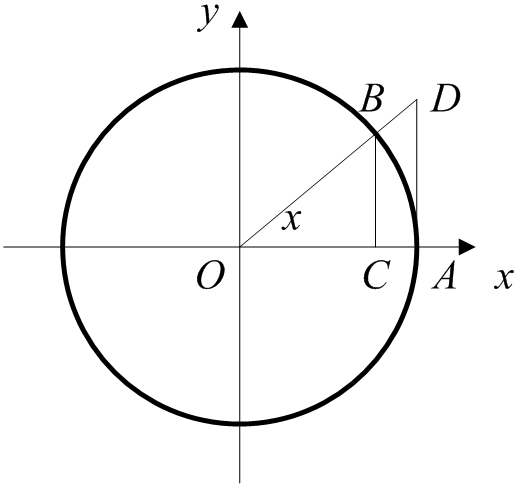
\includegraphics[height=3.5cm]{1.1.png}
\end{figure}

考虑单位圆,{\it OD}和{\it x}轴夹角 。
考察三角形{\it OBC}、扇形{\it OAB}、三角形{\it OAD},三者面积有关系:
\begin{align*}
&\because S_{OBC}<S_{OAB}<S_{OAD} \\
&\therefore \frac{1}{2}\sin x\cos x<\pi \cdot \frac{x}{2\pi}<\frac{1}{2}\tan x \\
&\therefore \cos x<\frac{\sin x}{x}<\frac{1}{\cos x}
\end{align*}
对于余弦函数有$\underset{x\rightarrow 0}{\lim}\cos x=1$,由夹逼定理得:
\[
\underset{x\rightarrow 0}{\lim}\frac{\sin x}{x}=1
\]

注意,这里不能用线段{\it BC}长度、弧{\it AB}长度、线段{\it AD}长度的关系$BC<\overset\frown{AB}<AD$。
因为$\overset\frown{AB}<AD$不是那么显而易见,需要证明。

\begin{tcolorbox}
该极限将三角函数和多项式函数联系起来。
其值是一个计算得到的数值。
\end{tcolorbox}

{\bf 计算$\underset{x\rightarrow \infty}{\lim}\left( 1+\frac{1}{x} \right) ^x$}

还是用夹逼定理。
构造一个数列$x_n=\left( 1+\frac{1}{n} \right) ^n$。
用有界定理推导极限$\underset{n\rightarrow \infty}{\lim}\left\{ x_n \right\} $存在,证明略,并记为$e$。
\begin{align*}
&\because x>0\Rightarrow n\leqslant x\leqslant n+1 \\
&\therefore \left( 1+\frac{1}{1+n} \right) ^n<\left( 1+\frac{1}{x} \right) ^n\leqslant \left( 1+\frac{1}{x} \right) ^x\leqslant \left( 1+\frac{1}{n} \right) ^x<\left( 1+\frac{1}{n} \right) ^{n+1} \\
&\because \begin{cases}
	\underset{n\rightarrow \infty}{\lim}\left( 1+\frac{1}{1+n} \right) ^n=\underset{n\rightarrow \infty}{\lim}\frac{\left( 1+\frac{1}{1+n} \right) ^{n+1}}{1+\frac{1}{1+n}}=e\\
	\underset{n\rightarrow \infty}{\lim}\left( 1+\frac{1}{n} \right) ^{1+n}=\underset{n\rightarrow \infty}{\lim}\left[ \left( 1+\frac{1}{1+n} \right) ^n\left( 1+\frac{1}{1+n} \right) \right] =e\\
\end{cases} \\
&\therefore \underset{x\rightarrow +\infty}{\lim}\left( 1+\frac{1}{x} \right) ^x=e
\end{align*}
同理可证明$\underset{x\rightarrow -\infty}{\lim}\left( 1+\frac{1}{x} \right) ^x=e$。
由左右极限存在且相等得该极限存在且:
\[
\underset{x\rightarrow \infty}{\lim}\left( 1+\frac{1}{x} \right) ^x
\]

\begin{tcolorbox}
注意,该极限的值$e$是一个定义值。
该极限把指数函数和幂函数联系起来。
对于幂指函数的极限,基本都会有$e$的影子。
\end{tcolorbox}






\newpage
\section{无穷小量和无穷大量}

本节给出无穷小量的概念,是微分的基础概念。

本节要点:
\begin{itemize}
    \item 理解无穷小量和无穷大量的概念;
    \item 理解本节最后一条定理。
\end{itemize}

%============================================================
\subsection{无穷量的概念}

\begin{definition}[无穷小量]
若$\forall \varepsilon >0$时存在$\delta >0$,当$x\in N\left( \hat{x}_0,\delta \right) $时有$\left| f\left( x \right) -0 \right|<\varepsilon $,则称$f\left( x \right) $为{\bf 当$x\rightarrow x_0$时的无穷小量},记作
\[
\underset{x\rightarrow x_0}{\lim}f\left( x \right) =0
\]
\end{definition}

注意:0是一个特殊的无穷小量,也是唯一可以作为无穷小量的常数。

\begin{definition}[无穷大量]
若$\forall M>0$时存在$\delta >0$,当$x\in N\left( \hat{x}_0,\delta \right) $时有$\left| f\left( x \right) -0 \right|>M$,则称$f\left( x \right) $为{\bf 当$x\rightarrow x_0$时的无穷大量},记作
\[
\underset{x\rightarrow x_0}{\lim}f\left( x \right) =\infty
\]
\end{definition}

本质上,无穷小量和无穷大量都是极限,是函数的趋势。

%============================================================
\subsection{无穷量的定理}

\begin{theorem}[互倒定理]
在自变量趋向一致下,无穷小量和无穷大量互为倒数。
\end{theorem}

\begin{theorem}[有限和定理]
有限个无穷小量之和(差)仍为无穷小量。
\end{theorem}

\begin{theorem}[有限积定理]
有限个无穷小量之积仍为无穷小量。
\end{theorem}

\begin{theorem}[有界积定理]
若$\underset{x\rightarrow x_0}{\lim}f\left( x \right) =0$,$g\left( x \right) $在$x_0$的某去心邻域内有界,则$\underset{x\rightarrow x_0}{\lim}\left[ f\left( x \right) \cdot g\left( x \right) \right] =0$。
\end{theorem}

\begin{theorem}
$\underset{x\rightarrow x_0}{\lim}f\left( x \right) =A\Leftrightarrow f\left( x \right) =A+o\left( x \right) $,其中$A$为常数,$o\left( x \right) $为无穷小量,即$\underset{x\rightarrow x_0}{\lim}o\left( x \right) =0$。
\end{theorem}

最后一条定理反映的是极限运算,也是后续微分和近似分析的基础。

%============================================================
\subsection{无穷小的比较}

\begin{definition}
设$\underset{x\rightarrow x_0}{\lim}\alpha \left( x \right) =0,\underset{x\rightarrow x_0}{\lim}\beta \left( x \right) =0,\beta \left( x \right) \ne 0$ ,则可有如下定义:
\begin{itemize}
    \item 若有$\underset{x\rightarrow x_0}{\lim}\frac{\alpha \left( x \right)}{\beta \left( x \right)}=0$,则称当$x\rightarrow x_0$时,{\bf $\alpha \left( x \right) $是$\beta \left( x \right) $的高阶无穷小量},或{\bf $\beta \left( x \right) $是$\alpha \left( x \right) $的低阶无穷小量},记作$\alpha \left( x \right) =o\left( \beta \left( x \right) \right) $,
    \item 若有$\underset{x\rightarrow x_0}{\lim}\frac{\alpha \left( x \right)}{\beta \left( x \right)}=C\ne 0$,则称当$x\rightarrow x_0$时,{\bf $\alpha \left( x \right) $和$\beta \left( x \right) $是同阶无穷小量},特别地,如$C=1$,则称{\bf $\alpha \left( x \right) $和$\beta \left( x \right) $是等价无穷小},记作$\alpha \left( x \right) \sim \beta \left( x \right) $,
    \item 若$\underset{x\rightarrow x_0}{\lim}\frac{\alpha \left( x \right)}{\left[ \beta \left( x \right) \right] ^k}=C\ne 0,k>0$则称当$x\rightarrow x_0$时,{\bf $\alpha \left( x \right) $是$\beta \left( x \right) $的$k$阶无穷小量}。
\end{itemize}
\end{definition}

无穷小量的比较的数学意义是描述谁的趋近速度快。






\newpage
\section{光滑曲线的第一个要求}

对于好函数的要求——光滑,我们第一个直觉是“不能断”。

\begin{figure}[h]
\centering
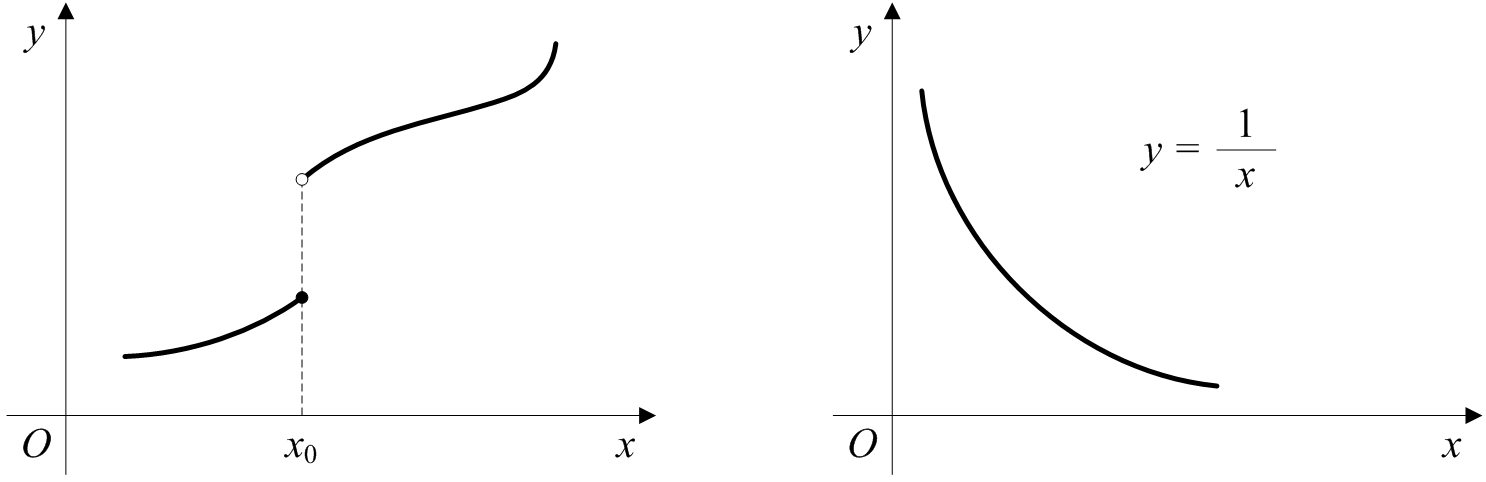
\includegraphics[height=3cm]{1.2.png}
\end{figure}

左上图的曲线不光滑,它“断了”。
右上图的曲线咋看没问题,但是在$x=0$处断了,不是人为地断,而是这个函数根本到不了断点。

那么什么是断,什么又不是断,我们需要给出一个数学上的“不断”的定义——连续。






\newpage
\section{连续}

本节给出的函数连续的定义,并给出连续的运算和定理。
最重要的是根据定理推导的一个重要的极限。

本节要点:
\begin{itemize}
    \item 理解连续的概念;
    \item 推导一个重要的极限:$\underset{x\rightarrow 0}{\lim}\frac{a^x-1}{x}=\ln a$。
\end{itemize}

%============================================================
\subsection{连续的概念}

\begin{definition}[连续]
设$f\left( x \right) $在某邻域$N\left( x_0 \right) $内有定义,若
\[
\underset{x\rightarrow x_0}{\lim}f\left( x \right) =f\left( x_0 \right)
\]
则称{\bf $f\left( x \right) $在点$x_0$处连续(continuity)}。
\end{definition}

连续在数学上规范了什么是“不断”。

\begin{definition}[区间连续]
若$f\left( x \right) $在开区间$\left( a,b \right) $内每一点连续,则称{\bf $f\left( x \right) $在开区间$\left( a,b \right) $连续},$\left( a,b \right) $称为$f\left( x \right) $的{\bf 连续区间},我们将$C\left( a,b \right) $表示$\left( a,b \right) $上所有连续函数构成的集合,则$f\left( x \right) \in C\left( a,b \right) $;若$f\left( x \right) $在开区间$\left( a,b \right) $连续,在点$a$右连续,在点$b$左连续,则称{\bf $f\left( x \right) $在闭区间$\left[ a,b \right] $连续}。
\end{definition}

\begin{definition}[一致连续性]
上面区间连续的定义中,当考察$\left| x-x_0 \right|<\delta $时,显然$\delta $可以和$x_0$有关。
当我们更严格地规定$\delta $仅和$\varepsilon $有关,与$x_0$具体在哪里无关时,称为$f\left( x \right) $在区间$\left( a,b \right) $(或$\left[ a,b \right] $){\bf 一致连续},或称{\bf 均匀连续}。
\end{definition}

\begin{definition}[间断点]
若$f\left( x \right) $在点$x_0$处不连续,则称$x_0$为$f\left( x \right) $的{\bf 间断点}。
\begin{itemize}
    \item 若$f\left( x \right) $在间断点$x_0$处左右极限均存在,称$x_0$为$f\left( x \right) $的{\bf 第一类间断点},
    \begin{itemize}
        \item 当左右极限不相等时,称为{\bf 跳跃型间断点},
        \item 当左右极限相等,但$x_0$未定义或$\underset{x\rightarrow x_0}{\lim}f\left( x \right) \ne f\left( x_0 \right) $时,称为{\bf 可去型间断点};
    \end{itemize}
    \item 反之,若$f\left( x \right) $在间断点$x_0$处左右极限均不存在,或有一个不存在,称$x_0$为$f\left( x \right) $的{\bf 第二类间断点},
    \begin{itemize}
        \item 当有某侧极限为无穷大时,称为{\bf 无穷型间断点},
        \item 当某一侧极限呈振荡,不收敛于一个值时,称为{\bf 振荡型间断点}。
    \end{itemize}
\end{itemize}
\end{definition}

间断点表示函数不连续,第一类间断点表示函数还是往那个值收敛的,第二类间断点则表示函数在那个点是发散的。
第一类间断点对积分没有影响,第二类间断点就可能无法积分了。

%============================================================
\subsection{连续的几何意义}

几何上,连续表示从一点画到另一点,笔不能离开纸面。
也就是说,变量从一个量到另一个量,必然通过中间的某个量。
再看下面两个断的曲线。
左图在$x=x_0$时是有值的,但是笔在该点腾空了,反映在连续上,左右连续不是相等的。
右图在$x=0$时函数根本没有极限,或者说极限为$\infty $。

\begin{figure}[h]
\centering
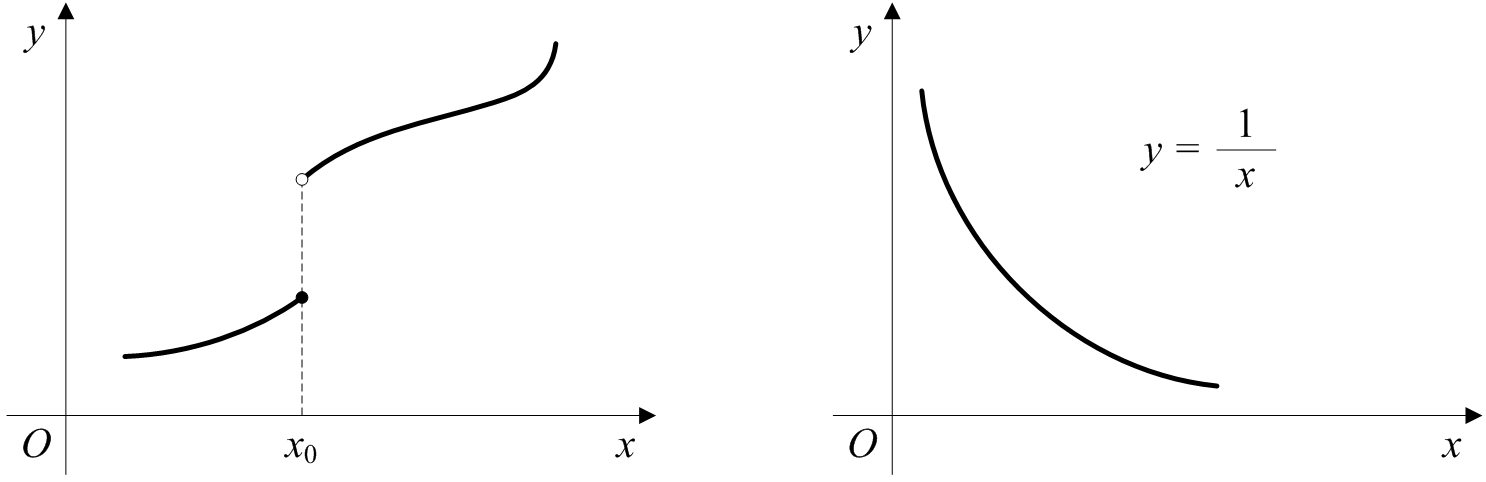
\includegraphics[height=3cm]{1.2.png}
\end{figure}

基于这个几何意义,连续的运算法则和几个定理也是非常容易理解,且不证自明。

%============================================================
\subsection{连续的运算法则}

若$f\left( x \right) ,g\left( x \right) $在点$x_0$处连续,则有
\begin{align*}
&C\cdot f\left( x \right) \\
&f\left( x \right) \pm g\left( x \right) \\
&f\left( x \right) \cdot g\left( x \right) \\
&\frac{f\left( x \right)}{g\left( x \right)}
\end{align*}
且在点$x_0$处连续。
特别注意1、2两式表明连续也是线性的。

%============================================================
\subsection{连续的定理}

\begin{theorem}[初等函数连续定理]
基本初等函数和初等函数在其定义域的区间上是连续的。
\end{theorem}

\begin{theorem}[反函数的连续性]
若函数$f\left( x \right) $在某区间内连续且单调,则其反函数$f^{-1}\left( x \right) $在原函数对应的值域内连续且单调,且具有相同的单调性。
\end{theorem}

\begin{theorem}[复合函数的连续性]
若$\underset{x\rightarrow x_0}{\lim}\varphi \left( x \right) =\varphi \left( x_0 \right) =u_0$,$\underset{u\rightarrow u_0}{\lim}f\left( u \right) =f\left( u_0 \right) $,则
\[
\underset{x\rightarrow x_0}{\lim}f\left( \varphi \left( x \right) \right) =f\left( \underset{x\rightarrow x_0}{\lim}\varphi \left( x \right) \right) =f\left( \varphi \left( x_0 \right) \right)
\]
\end{theorem}

该定理表示极限符号和函数符号可以交换顺序。
初等函数连续定理和该定理常用于计算极限。

\begin{theorem}[最值定理]
若$f\left( x \right) $在闭区间$\left[ a,b \right] $连续,则必在$\left[ a,b \right] $上有最大值和最小值。
\end{theorem}

\begin{theorem}[有界定理]
若$f\left( x \right) $在闭区间$\left[ a,b \right] $连续,则必在$\left[ a,b \right] $上有界。
\end{theorem}

\begin{theorem}[介值定理]
若$f\left( x \right) $在闭区间$\left[ a,b \right] $连续,且$f\left( a \right) \ne f\left( b \right) $,则对于任何$\forall \mu \in \left[ f\left( a \right) ,f\left( b \right) \right] $或$\forall \mu \in \left[ f\left( b \right) ,f\left( a \right) \right] $,必存在$\xi \in \left[ a,b \right] $,使得$f\left( \xi \right) =\mu $。几何上表示曲线$y=f\left( x \right) $和直线$y=\mu $至少有一个交点。
\end{theorem}

\begin{corollary}
若$f\left( x \right) $在闭区间$\left[ a,b \right] $连续,且有最大值和最小值$m,M$,则对于任何$\forall \mu \in \left[ m,M \right] $,必存在$\xi \in \left[ a,b \right] $,使得$f\left( \xi \right) =\mu $。
\end{corollary}

\begin{corollary}[根存在定理]
若$f\left( x \right) $在闭区间$\left[ a,b \right] $连续,且$f\left( a \right) \cdot f\left( b \right) <0$,则必存在$\xi \in \left[ a,b \right] $,使得$f\left( \xi \right) =0$。
\end{corollary}

\begin{corollary}[唯一根存在定理]
若$f\left( x \right) $在闭区间$\left[ a,b \right] $连续且严格单调,且$f\left( a \right) \cdot f\left( b \right) <0$,则有唯一$\xi \in \left[ a,b \right] $,使得$f\left( \xi \right) =0$。
\end{corollary}

最值定理和有界定理是等价的。

%============================================================
\subsection{两个重要的极限}

{\bf 计算$\underset{x\rightarrow 0}{\lim}\frac{\log _a\left( 1+x \right)}{x}$}

首先有
\[
\frac{\log _a\left( 1+x \right)}{x}=\log _a\left( 1+x \right) ^{\frac{1}{x}}
\]
然后运用复合函数的连续性定理:
\[
\underset{x\rightarrow 0}{\lim}\log _a\left( 1+x \right) ^{\frac{1}{x}}=\log _a\underset{x\rightarrow 0}{\lim}\left( 1+x \right) ^{\frac{1}{x}}=\log _ae=\frac{\ln e}{\ln a}=\frac{1}{\ln a}
\]
特别的,当$a=e$时:
\[
\underset{x\rightarrow 0}{\lim}\frac{\ln \left( 1+x \right)}{x}=1
\]

{\bf 计算$\underset{x\rightarrow 0}{\lim}\frac{a^x-1}{x}$}

令$a^x-1=t$,得$x=\log _a\left( t+1 \right) $,且$x\rightarrow 0$时有$t\rightarrow 0$,所以:
\[
\underset{x\rightarrow 0}{\lim}\frac{a^x-1}{x}=\underset{x\rightarrow 0}{\lim}\frac{t}{\log _a\left( t+1 \right)}=\underset{x\rightarrow 0}{\lim}\frac{1}{\log _a\left( t+1 \right) ^{1/t}}=\ln a
\]
特别的,当$a=e$时:
\[
\underset{x\rightarrow 0}{\lim}\frac{e^x-1}{x}=1
\]

\begin{tcolorbox}
该极限在求解指数函数$a^x$的导数时用到,是三大基本导数之一。
\end{tcolorbox}

%============================================================
\subsection{再论四个重要极限}

以下四个重要极限揭示了基本初等函数之间的关系:

\begin{table}[h]
\centering
\begin{tabular}{lc}
    \toprule
    极限 & 函数间的联系\\
    \midrule
    $\underset{x\rightarrow 0}{\lim}\frac{\sin x}{x}=1$ & 联系了幂函数和三角函数。\\
    $\underset{x\rightarrow \infty}{\lim}\left( 1+\frac{1}{x} \right) ^x=e$ & 联系了幂函数和指数函数。\\
    $\underset{x\rightarrow 0}{\lim}\frac{\log _a\left( 1+x \right)}{x}=\frac{1}{\ln a}$ & 联系了幂函数和对数函数。\\
    $\underset{x\rightarrow 0}{\lim}\frac{a^x-1}{x}=\ln a$ & 联系了幂函数和指数函数。\\
    \bottomrule
\end{tabular}
\end{table}






\newpage
\section{本章小结}

形而下来讲,本章最重要的概念是“极限”及其运算,是后续章节的基础。
形而上来讲,本章最重要的是“连续”。
因为我们的目标是理解“光滑”的好函数。
什么是光滑,通过连续这个数学概念,严格地、量化地规定了光滑的第一个要求——不断。






\newpage
\section{习题}

\begin{exercise}
求下列极限:
\begin{enumerate}
    \item $\underset{x\rightarrow -2}{\lim}\frac{x^2-x+2}{x^2+4}$
    \item $\underset{x\rightarrow 1}{\lim}\left( \frac{1}{1-x}-\frac{3}{1-x^2} \right) $
    \item $\underset{x\rightarrow 0}{\lim}\frac{\left| 2x-1 \right|-\left| 2x+1 \right|}{x}$
    \item $\underset{x\rightarrow 0}{\lim}\frac{x-\sin 2x}{x+\sin 5x}$
    \item $\underset{x\rightarrow \infty}{\lim}\left( \frac{x-4}{x+1} \right) ^{2x-1}$
    \item $\underset{x\rightarrow \infty}{\lim}\sin \left( 1+\frac{1}{x} \right) ^{2x+1}$
    \item $\underset{x\rightarrow \infty}{\lim}\lg \frac{100+x^2}{1+100x^2}$
\end{enumerate}
\end{exercise}

解:

1.
\[
\underset{x\rightarrow -2}{\lim}\frac{x^2-x+2}{x^2+4}=\left. \frac{x^2-x+2}{x^2+4} \right|_{x=-2}=1
\]

2.
\[
\underset{x\rightarrow 1}{\lim}\left( \frac{1}{1-x}-\frac{3}{1-x^2} \right) =\underset{x\rightarrow 1}{\lim}\frac{\left( x+2 \right) \left( x-1 \right)}{1-x^3}=-\underset{x\rightarrow 1}{\lim}\frac{x+2}{x^2+x+1}=-1
\]

3.
\[
\underset{x\rightarrow 0}{\lim}\frac{\left| 2x-1 \right|-\left| 2x+1 \right|}{x}=\underset{x\rightarrow 0}{\lim}\frac{\left( 1-2x \right) -\left( 2x+1 \right)}{x}=\underset{x\rightarrow 0}{\lim}\frac{-4x}{x}=-4
\]

4.
\[
\underset{x\rightarrow 0}{\lim}\frac{x-\sin 2x}{x+\sin 5x}=\underset{x\rightarrow 0}{\lim}\frac{1-2\frac{\sin 2x}{2x}}{1+5\frac{\sin 5x}{5x}}=-\frac{1}{6}
\]

5.
\begin{align*}
&\underset{x\rightarrow \infty}{\lim}\left( \frac{x-4}{x+1} \right) ^{2x-1}=\underset{x\rightarrow \infty}{\lim}\left( 1+\frac{-5}{x+1} \right) ^{2\left( x+1 \right) -3} \\
&=\underset{x\rightarrow \infty}{\lim}\left( 1+\frac{-10}{2\left( x+1 \right)} \right) ^{2\left( x+1 \right)}\cdot \underset{x\rightarrow \infty}{\lim}\left( 1-10\frac{1}{2\left( x+1 \right)} \right) ^{-3} \\
&=\underset{t\rightarrow \infty}{\lim}\left( 1+\frac{-10}{t} \right) ^t\cdot 1^{-3}=e^{-10}
\end{align*}

6.
\begin{align*}
&\underset{x\rightarrow \infty}{\lim}\sin \left[ \left( 1+\frac{1}{x} \right) ^{2x+1} \right] =\sin \underset{x\rightarrow \infty}{\lim}\left( 1+\frac{2}{2x} \right) ^{2x+1} \\
&=\sin \left[ \underset{x\rightarrow \infty}{\lim}\left( 1+\frac{2}{2x} \right) ^{2x}\cdot \underset{x\rightarrow \infty}{\lim}\left( 1+\frac{2}{2x} \right) ^1 \right] =\sin \left( e^2\cdot 1 \right)
\end{align*}

7.
\[
\underset{x\rightarrow \infty}{\lim}\lg \frac{100+x^2}{1+100x^2}=\lg \underset{x\rightarrow \infty}{\lim}\frac{100+x^2}{1+100x^2}=\lg \frac{1}{100}=-2
\]

\begin{tcolorbox}
本题还是以直接带入为主,有些小题需要化简一下式子而已。
\end{tcolorbox}

~

\begin{exercise}
求$\underset{x\rightarrow +\infty}{\lim}\left( \sin \sqrt{x+1}-\sin \sqrt{x} \right) $。
\end{exercise}

解:

总体思路是将两个三角函数合并到一个,然后考察三角函数内多项式的极限。

首先化简三角函数:
\[
\underset{x\rightarrow +\infty}{\lim}\left( \sin \sqrt{x+1}-\sin \sqrt{x} \right) =\underset{x\rightarrow +\infty}{\lim}2\cos \frac{\sqrt{x+1}+\sqrt{x}}{2}\sin \frac{\sqrt{x+1}-\sqrt{x}}{2}
\]
然后考察$\cos \frac{\sqrt{x+1}+\sqrt{x}}{2}$,是有界函数,再考察$\sin \frac{\sqrt{x+1}-\sqrt{x}}{2}$,当$x\rightarrow \infty $时似乎$\sqrt{x+1}-\sqrt{x}\rightarrow 0$:
\begin{align*}
&\because \frac{\sqrt{x+1}-\sqrt{x}}{2}=\frac{1}{2\left( \sqrt{x+1}+\sqrt{x} \right)} \\
&\therefore \underset{x\rightarrow +\infty}{\lim}\sin \frac{\sqrt{x+1}-\sqrt{x}}{2}=\sin \underset{x\rightarrow +\infty}{\lim}\frac{1}{2\left( \sqrt{x+1}+\sqrt{x} \right)}=\sin 0=0
\end{align*}
所以:
\[
\underset{x\rightarrow +\infty}{\lim}\left( \sin \sqrt{x+1}-\sin \sqrt{x} \right) =\underset{x\rightarrow +\infty}{\lim}\left( 2\cos \frac{\sqrt{x+1}+\sqrt{x}}{2}\cdot 0 \right) =0
\]

~

\begin{exercise}
若
\[
\begin{cases}
	\underset{x\rightarrow a}{\lim}\left[ f\left( x \right) +g\left( x \right) \right] =2\\
	\underset{x\rightarrow a}{\lim}\left[ f\left( x \right) -g\left( x \right) \right] =1\\
\end{cases}
\]
求$\underset{x\rightarrow a}{\lim}\left[ f\left( x \right) \cdot g\left( x \right) \right] $。
\end{exercise}

解:

总体思路是采用极限的线性组合。
\begin{align*}
&\because \begin{cases}
	\underset{x\rightarrow a}{\lim}\left[ f+g \right] ^2=\underset{x\rightarrow a}{\lim}\left[ f^2+g^2+2fg \right] =4\\
	\underset{x\rightarrow a}{\lim}\left[ f-g \right] ^2=\underset{x\rightarrow a}{\lim}\left[ f^2+g^2-2fg \right] =1\\
\end{cases} \\
&\therefore \underset{x\rightarrow a}{\lim}fg=\frac{1}{4}\left( 4-1 \right) =\frac{3}{4}
\end{align*}

~

\begin{exercise}
若有方程$x^3-3x=1$,讨论其在$\left[ 1,2 \right] $上有无根。
\end{exercise}

解:

总体思路是考察连续函数的根存在定理。

令$y=x^3-3x-1$,则$y$在$\left[ 1,2 \right] $上连续,且:
\[
y\left( 1 \right) \cdot y\left( 2 \right) =-3<0
\]
根据根存在定理,必有根。

~

\begin{exercise}
如下图,等边三角形内放置直径相同的若干个圆,图示为10个,三角形外切圆。当增大圆的个数时,能否覆盖三角形,如能则最终需要多少个,如不能,则最终能覆盖多少三角形面积。
\begin{figure}[h]
\centering
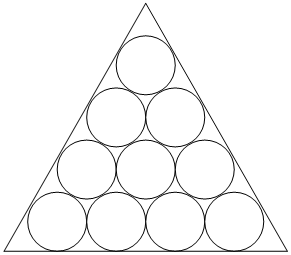
\includegraphics[height=2.5cm]{1.3.png}
\end{figure}
\end{exercise}

解:

总体思路是考察圆的总面积和三角形面积的比例的极限。

假设三角形面积$A$,所有圆面积之和$A_n$,圆半径$r$,一边放$n$个,一共$\frac{1}{2}n\left( n-1 \right) $个圆。于是所有圆面积之和$A_n$为:
\[
A_n=\pi r^2\cdot \frac{1}{2}n\left( n+1 \right)
\]
易得三角形边长$L=2\left( n-1 \right) r+2\sqrt{3}\cdot r$,于是三角形面积$A$为:
\[
A=\frac{1}{2}\cdot L\cdot \frac{\sqrt{3}}{2}L=\frac{\sqrt{3}}{4}\left[ 2\left( n-1 \right) r+2\sqrt{3}r \right] ^2
\]
于是:
\[
\underset{n\rightarrow \infty}{\lim}\frac{A_n}{A}=\underset{n\rightarrow \infty}{\lim}\frac{\pi r^2\cdot \frac{1}{2}n\left( n+1 \right)}{\frac{\sqrt{3}}{4}\left[ 2\left( n-1 \right) r+2\sqrt{3}r \right] ^2}=\frac{\pi r^2\cdot \frac{1}{2}}{\frac{\sqrt{3}}{4}\cdot 4r^2}=\frac{\pi}{2\sqrt{3}}=0.9069
\]
最多只能覆盖三角形的90\%多一点的面积。










\chapter{一元函数微分学}

在工程技术或对物理的研究中,通常要知道一个运动的趋势,能不能达到某一点,变化过程是否均匀,趋向什么状态等。
要解决这类问题,需要对函数的变化和趋势进行研究,导数和微分就是解决这类问题的工具。

从微积分的两个对立概念“微分”和“积分”来看,微分是从变化的角度考察函数,积分是从累积的角度考察函数。

对于导数:
\begin{itemize}
    \item 充分理解其数学定义、几何意义和物理意义。
    \item 熟练掌握导数基本公式、复合函数、隐函数和参数式函数的求导方法。
    \item 掌握洛必达法则,学会用该法则求解不定型的极限。
    \item 学会推导三个基本导数公式。
    \item 理解和掌握麦克劳林公式,学会用麦克劳林公式将超越方程转化为多项式方程求解工程问题。
\end{itemize}

对于微分:
\begin{itemize}
    \item 充分理解微分的数学定义、几何意义和物理意义。
    \item 理解微分和导数的关系,并能证明微分定理。
    \item 学会使用微分求解工程上的近似问题。
\end{itemize}

\newpage
\section{光滑曲线的第二个要求}

上一章讨论了光滑的第一个要求——不断,本章讨论我们定义光滑的第二个要求——不折。
如下曲线,在$x_0$处折了。

\begin{figure}[h]
\centering
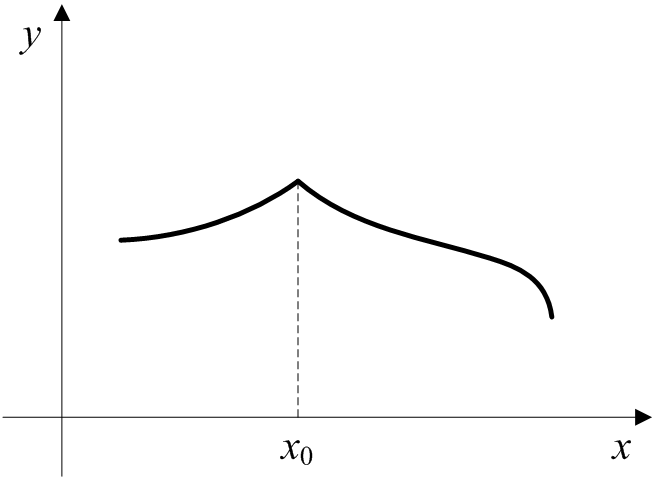
\includegraphics[height=4cm]{2.1.png}
\end{figure}






\newpage
\section{导数}

本节给出导数的概念。
着重理解导数,并使用概念证明函数的可导性。

本节要点:
\begin{itemize}
    \item 理解导数概念;
    \item 熟练掌握初等函数的导数公式表;
    \item 掌握四类函数(复合函数、反函数、隐函数、参数式函数)的求导方法。
\end{itemize}

%============================================================
\subsection{导数的概念}

\begin{definition}[增量]
函数表示了两个变量(自变量和因变量)之间的关系。我们定义,{\bf 自变量的增量}是两个自变量的差,{\bf 因变量的增量}是两个因变量的差,即:
\begin{align*}
&\Delta x:=x_1-x_0 \\
&\Delta y:=y_1-y_0=f\left( x_1 \right) -f\left( x_0 \right)
\end{align*}
\end{definition}

\begin{definition}[变化率]
我们定义两个增量的比值为{\bf 函数的变化率},即:
\[
\frac{\Delta y}{\Delta x}=\frac{f\left( x_1 \right) -f\left( x_0 \right)}{x_1-x_0}=\frac{f\left( x_0+\Delta x \right) -f\left( x_0 \right)}{\Delta x}
\]
\end{definition}

显然,函数的变化率是一个和自变量及其增量区间有关的新函数。
当取相同的$\Delta x$时,变化率描述了函数的变化快慢。
变化率越大,说明函数在同等$\Delta x$下的变化越大。

下面我们考察函数在一个点上的变化率,即当$x_1\rightarrow x_0$(或$\Delta x\rightarrow 0$),函数的变化率的存在性和取值。

\begin{definition}[导数]
设函数$f\left( x \right) $在点$x_0$的某邻域$N\left( x_0 \right) $内有定义,若当$\Delta x\rightarrow 0$时$\Delta y/\Delta x$的极限存在,则称{\bf 函数$f\left( x \right) $在$x_0$处可导},并称此极限值为{\bf 函数$f\left( x \right) $在点$x_0$的导数(derivative)},记为$f'\left( x_0 \right) $,即:
\[
f'\left( x_0 \right) :=\underset{\Delta x\rightarrow 0}{\lim}\frac{\Delta y}{\Delta x} \quad \text{或} \quad f'\left( x_0 \right) :=\underset{x_1\rightarrow x_0}{\lim}\frac{f\left( x_1 \right) -f\left( x_0 \right)}{x_1-x_0}
\]
也可用莱布尼兹(Leibniz)记号记为:
\[
\left. y' \right|_{x=x_0} \quad \text{或} \quad \left. \frac{dy}{dx} \right|_{x=x_0}
\]
\end{definition}

从定义上来讲,函数$f\left( x \right) $在$x_0$处的导数是一个极限,是一个可计算的确定的数。

\begin{definition}[左导数]
设函数$f\left( x \right) $在点$x_0$的左邻域$\left( x_0-\delta ,x_0 \right) $内有定义,若当$\Delta x\rightarrow 0^-$时$\Delta y/\Delta x$的极限存在,则称{\bf 函数$f\left( x \right) $在点$x_0$处左可导},并称此极限值为{\bf 函数$f\left( x \right) $在点$x_0$处的左导数},记为$f'_-\left( x_0 \right) $,即:
\[
f'_-\left( x_0 \right) :=\underset{\Delta x\rightarrow 0^-}{\lim}\frac{\Delta y}{\Delta x}=\underset{x_1\rightarrow {x_0}^-}{\lim}\frac{f\left( x_1 \right) -f\left( x_0 \right)}{x_1-x_0}
\]
\end{definition}

\begin{definition}[右导数]
设函数$f\left( x \right) $在点$x_0$的右邻域$\left( x_0,x_0+\delta \right) $内有定义,若当$\Delta x\rightarrow 0^+$时$\Delta y/\Delta x$的极限存在,则称{\bf 函数$f\left( x \right) $在点$x_0$处右可导},并称此极限值为{\bf 函数$f\left( x \right) $在点$x_0$处的右导数},记为$f'_+\left( x_0 \right) $,即:
\[
f'_+\left( x_0 \right) :=\underset{\Delta x\rightarrow 0^+}{\lim}\frac{\Delta y}{\Delta x}=\underset{x_1\rightarrow {x_0}^+}{\lim}\frac{f\left( x_1 \right) -f\left( x_0 \right)}{x_1-x_0}
\]
\end{definition}

\begin{definition}[导函数]
如果函数$f\left( x \right) $在区间$D$内每一点都可导,则称每个导数构成的新函数为{\bf $f\left( x \right) $的导函数},记为$f'\left( x \right) $(或$y'$)。
显然,导函数$f'\left( x \right) $在$x_0$的值就是导数$f'\left( x_0 \right) $。
\end{definition}

除非特别指明,一般我们将导函数简称为导数。
区间$\left( a,b \right) $(或$\left[ a,b \right] $)内所有可导函数的集合通常记作$D\left( a,b \right) $(或$D\left[ a,b \right] $),所以$f\left( x \right) $在区间$D$内可导也可记作$f\left( x \right) \in D\left( a,b \right) $(或$f\left( x \right) \in D\left[ a,b \right] $)。

求导是对函数的一种运算。
运算对象是函数,得到的结果是另一个函数。
从集合角度,求导是一个函数集合到另一个函数集合的映射。

\begin{tcolorbox}
在讨论导数的时候,紧紧抓住导数的定义,从定义出发。
后续关于导数的定理和公式都是用定义证明和推导。
\end{tcolorbox}

%============================================================
\subsection{导数的几何意义}

考察如下曲线。
\begin{figure}[h]
\centering
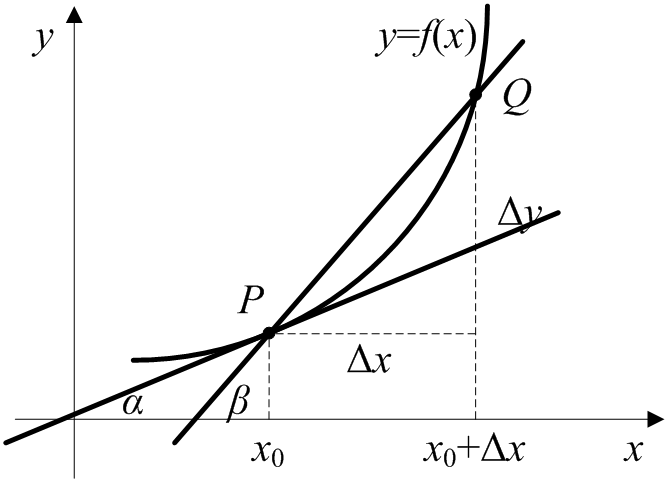
\includegraphics[height=4cm]{2.2.png}
\end{figure}

函数在{\it PQ}之间的变化率在几何上体现为割线{\it PQ}的斜率:
\[
\tan \beta =\frac{\Delta y}{\Delta x}
\]
函数在{\it P}点上的变化率在几何上体现为曲线在{\it P}点处的切线的斜率:
\[
\tan \alpha =\underset{\Delta x\rightarrow 0}{\lim}\frac{\Delta y}{\Delta x}=f'\left( x_0 \right)
\]
如果曲线沿着左右两个方向靠近{\it P}点时的切线斜率是一样的,就说明该点不折。
再看本章一开始的曲线,该曲线在$x_0$处左右导数都是有的,但不相等。
\begin{figure}[ht]
\centering
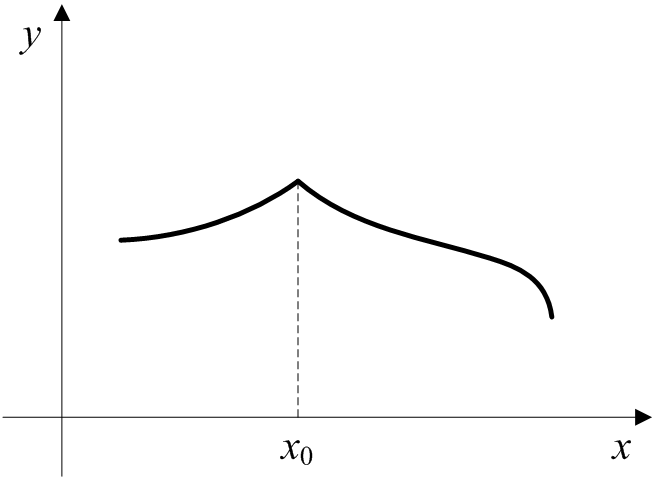
\includegraphics[height=4cm]{2.1.png}
\end{figure}

从几何上来讲,导数的意义是切线的斜率。
反映到光滑上,导数给出了对光滑的第二要求“不折”的数学定义。

%============================================================
\subsection{曲线的切线和法线}

我们将导数这个工具应用到曲线的分析上,分析曲线上任意一点处的切线和法线。

曲线在代数上可以定义为函数$y=f\left( x \right) ,x\in D$。现在我们已知曲线上任何一点$\left( x_0,y_0 \right) $处的斜率就是该点处的导数$f'\left( x_0 \right) $,于是我们得到了曲线上任意一点处的切线和法线的粗略的表达式:
\begin{align*}
&y_{tangent}=f'\left( x_0 \right) x+c \\
&y_{normal}=-\frac{1}{f'\left( x_0 \right)}x+c
\end{align*}
将点$\left( x_0,y_0 \right) $带入即可求得$c$,最终得到切线和法线方程如下:
\begin{align*}
&y_{tangent}=f'\left( x_0 \right) x+\left[ f\left( x_0 \right) -f'\left( x_0 \right) x_0 \right] \\
&y_{normal}=-\frac{1}{f'\left( x_0 \right)}x+\left[ f\left( x_0 \right) +\frac{1}{f'\left( x_0 \right)}x_0 \right]
\end{align*}

%============================================================
\subsection{导数的物理意义}

物理上,导数描述了一个物理量的瞬时变化速度。
比方说路程的导数是速度,速度的导数是加速度。
导数为求解物理量的变化速度提供了强大的数学工具。

有的时候,我们知道两个物理量之间的关系和其中一个物理量的变化率,通过导数就可以得到另一个物理量的变化率。
实际问题中,前者的变化率已知且简单,后者变化率复杂,无法直接获得,通过这个方法就可以获得一个复杂的、不直观的变化率。
换一种说法,我们要获得一个物理量的变化率,但该变化率复杂,难以通过常规的方法求解。
我们可以将它关联到一个具有简单已知的变化率的物理量,通过导数的运算和求导法则计算得到,比如观测仰角的变化率。

%============================================================
\subsection{导数的定理}

\begin{theorem}
$f\left( x \right) $在$x_0$处可导$\Leftrightarrow f\left( x \right) $在$x_0$处左右导数存在且相等,即$f'_-\left( x_0 \right) =f'_+\left( x_0 \right) $。
\end{theorem}

\begin{theorem}
$f\left( x \right) $在$x_0$处可导$\Leftrightarrow f\left( x \right) $在$x_0$处连续。
\end{theorem}

\begin{proof}
从连续的定义出发,即证明$\underset{x\rightarrow x_0}{\lim}\left[ f\left( x \right) -f\left( x_0 \right) \right] =0$。
\begin{align*}
\underset{x\rightarrow x_0}{\lim}\left[ f\left( x \right) -f\left( x_0 \right) \right] &=\underset{x\rightarrow x_0}{\lim}\frac{f\left( x \right) -f\left( x_0 \right)}{x-x_0}\cdot \left( x-x_0 \right) \\
&=f'\left( x_0 \right) \underset{x\rightarrow x_0}{\lim}\left( x-x_0 \right) =0
\end{align*}
\end{proof}

%============================================================
\subsection{导数的四则运算}

\begin{align*}
&\left( C\cdot f \right) '=C\cdot f' \\
&\left( f\pm g \right) '=f'\pm g' \\
&\left( f\cdot g \right) '=f'g+fg' \\
&\left( \frac{f}{g} \right) '=\frac{f'g-fg'}{g^2} \\
&\left( \frac{1}{g} \right) '=-\frac{g'}{g^2}
\end{align*}

前两个公式表明导数运算是线性的。

%============================================================
\subsection{导数的基本公式}

\begin{align*}
\begin{matrix}
	\left( C \right) '=0 \hfill                                       & \left( x^a \right) '=a\cdot x^{a-1} \hfill \\
	\left( a^x \right) '=a^x\ln a \hfill                              & \left( e^x \right) '=e^x \hfill \\
	\left( \log _ax \right) '=\frac{1}{x\ln a} \hfill                 & \left( \ln x \right) '=\frac{1}{x} \hfill \\
	\left( \sin x \right) '=\cos x \hfill                             & \left( \cos x \right) '=-\sin x \hfill \\
	\left( \tan x \right) '=\sec ^2x \hfill                           & \left( \cot x \right) '=-\csc ^2x \hfill \\
	\left( \sec x \right) '=\sec x\cdot \tan x \hfill                 & \left( \csc x \right) '=-\csc x\cdot \cot x \hfill \\
	\left( \mathrm{arc}\sin x \right) '=\frac{1}{\sqrt{1-x^2}} \hfill & \left( \mathrm{arc}\cos x \right) '=-\frac{1}{\sqrt{1-x^2}} \hfill \\
	\left( \mathrm{arc}\tan x \right) '=\frac{1}{1+x^2} \hfill        & \left( \mathrm{arc}\cot x \right) '=-\frac{1}{1+x^2} \hfill \\
	\left( \mathrm{sh}x \right) '=\mathrm{ch}x \hfill                 & \left( \mathrm{ch}x \right) '=\mathrm{sh}x \hfill \\
\end{matrix}
\end{align*}

以上基本公式中,除了$\left( C \right) ',\left( a^x \right) ',\left( \sin x \right) '$,其余都可以从这三个公式导出。

{\bf 计算$\left( C \right) '$}
\[
\left( C \right) '=\underset{\Delta x\rightarrow 0}{\lim}\frac{C-C}{\Delta x}=0
\]

{\bf 计算$\left( a^x \right) '$}
\[
\left( a^x \right) '=\underset{\Delta x\rightarrow 0}{\lim}\frac{a^{x+\Delta x}-a^x}{\Delta x}=a^x\underset{\Delta x\rightarrow 0}{\lim}\frac{a^{\Delta x}-1}{\Delta x}=a^x\ln a
\]

{\bf 计算$\left( \sin x \right) '$}
\begin{align*}
\left( \sin x \right) '&=\underset{\Delta x\rightarrow 0}{\lim}\frac{\sin \left( x+\Delta x \right) -\sin x}{\Delta x} \\
&=\underset{\Delta x\rightarrow 0}{\lim}\frac{2\sin \frac{\Delta x}{2}\cos \frac{2x+\Delta x}{2}}{\Delta x}=\underset{\Delta x\rightarrow 0}{\lim}cos \frac{2x+\Delta x}{2}=\cos x
\end{align*}

%============================================================
\subsection{复合函数的求导}

\begin{theorem}[复合函数求导定理]
若函数$y=y\left( u \right) ,u=u\left( x \right) $在对应区间可导,则复合函数$y=y\left[ u\left( x \right) \right] $在对应区间也可导,且有:
\[
\frac{dy}{dx}=\frac{dy}{du}\cdot \frac{du}{dx}
\]
\end{theorem}

复合求导法则是接下去三种求导法则(反函数求导、隐函数求导、参数式函数求导)的基础。

%============================================================
\subsection{反函数的求导}

\begin{theorem}[反函数求导定理]
若函数$y=f\left( x \right) $在某区间内单调可导,且$y'\ne 0$,则它的反函数$x=f^{-1}\left( y \right) $在对应区间内也可导,且有:
\[
f'\left( x \right) =\frac{1}{\left( f^{-1} \right) '\left( y \right)}
\]
或写成:
\[
\frac{dy}{dx}=\frac{1}{\frac{dx}{dy}}
\]
\end{theorem}

\begin{proof}
\[
f'\left( x \right) =\underset{\Delta x\rightarrow 0}{\lim}\frac{\Delta y}{\Delta x}=\underset{\Delta x\rightarrow 0}{\lim}\frac{1}{\frac{\Delta x}{\Delta y}}=\frac{1}{\underset{\Delta y\rightarrow 0}{\lim}\frac{\Delta x}{\Delta y}}=\frac{1}{\left( f^{-1} \right) '\left( y \right)}
\]
\end{proof}

~

\begin{example}
设$y=\mathrm{arc}\sin x$,求$y'$。
\end{example}

解:

\[
\frac{dy}{dx}=\frac{1}{\frac{dx}{dy}}=\frac{1}{\left( \sin y \right) '}=\frac{1}{\cos y}=\frac{1}{\sqrt{1-\sin ^2y}}=\frac{1}{\sqrt{1-x^2}}
\]

%============================================================
\subsection{隐函数的求导}

\begin{theorem}[一元隐函数求导定理]
若方程$F\left( x,y \right) =0$确定唯一的单值连续可导函数$y=f\left( x \right) $,则有:
\[
\frac{dy}{dx}=-\frac{F_x}{F_y}
\]
其中:
\begin{itemize}
	\item $F_x$:表示$F\left( x,y \right) =0$对$x$求导,$x$是自变量,$y$是常量;
	\item $F_y$:表示$F\left( x,y \right) =0$对$y$求导,$y$是自变量,$x$是常量。
\end{itemize}
\end{theorem}


\begin{tcolorbox}
该定理在多元函数微积分中证明,这里只需知道如何计算一元隐函数的导数。
\end{tcolorbox}

~

\begin{example}
假设方程$e^y=e-xy$确定了函数$y=f\left( x \right) $,求$y'$。
\end{example}

解:

令$F\left( x,y \right) :=e^y-e+xy=0$,得:
\begin{align*}
&\because \begin{cases}
	F_x=y\\
	F_y=e^y+x\\
\end{cases} \\
&\therefore y'=-\frac{F_x}{F_y}=-\frac{y}{e^y+x}
\end{align*}

%============================================================
\subsection{参数式函数的求导}

\begin{theorem}[参数函数求导定理]
若参数方程
\begin{align*}
\begin{cases}
	x=x\left( t \right)\\
	y=y\left( t \right)\\
\end{cases}
\end{align*}
可导,$x=x\left( t \right) $存在可导的反函数,且$x'\left( t \right) \ne 0$,则由该参数方程确定的函数$y=f\left( x \right) $可导,且有:
\[
\frac{dy}{dx}=\frac{y'\left( t \right)}{x'\left( t \right)}
\]
\end{theorem}

~

\begin{example}
若有摆线
\begin{align*}
\begin{cases}
	x=t-\sin t\\
	y=1-\cos t\\
\end{cases}
\end{align*}
求$t=\pi /2$处的切线方程。
\end{example}

解:

切线方程$y=f'\left( x_0 \right) x+\left[ f\left( x_0 \right) -f'\left( x_0 \right) x_0 \right] $,可得:
\begin{align*}
&\left. \frac{dy}{dx} \right|_{t=\pi /2}=\left. \frac{dy}{dt}/\frac{dx}{dt} \right|_{t=\pi /2}=\left. \frac{\sin t}{1-\cos t} \right|_{t=\pi /2}=1 \\
&y=1\cdot x+\left[ \left( 1-\cos \frac{\pi}{2} \right) -1\cdot \left( \frac{\pi}{2}-1 \right) \right] =x+2-\frac{\pi}{2}
\end{align*}

%============================================================
\subsection{高阶导数}

\begin{definition}[二阶导数]
设函数$f\left( x \right) $在点$x_0$的某邻域$N\left( x_0 \right) $内可导,若极限
\[
\underset{\Delta x\rightarrow 0}{\lim}\frac{f'\left( x_0+\Delta x \right) -f'\left( x_0 \right)}{\Delta x}
\]
存在,则称该极限值为{\bf $f\left( x \right) $在点$x_0$处的二阶导数},记作:
\[
f''\left( x_0 \right) \quad \text{或} \quad \left. y'' \right|_{x=x_0} \quad \text{或} \quad \left. \frac{d^2y}{dx^2} \right|_{x=x_0}
\]
\end{definition}

同样,我们可以定义三阶导数、四阶导数、直至n阶导数。






\newpage
\section{微分}

本节给出微分概念。
着重理解微分及其意义和工程应用。

本节要点:
\begin{itemize}
    \item 熟练掌握微分概念;
    \item 学会推导微分定理。
\end{itemize}

~

工程上,经常碰到已知$f\left( x_0 \right) $,求$f\left( x_0+\Delta x \right) $的问题。
这个问题在数学上就是$\Delta y$能不能通过$\Delta x$的线性计算获得,误差多少,即:
\[
\Delta y=A\Delta x+B\left( \Delta x \right)
\]
且我们希望$A$与$\Delta x$无关,$B\left( \Delta x \right) $与$\Delta x$有关。

考虑这么几个问题:
\begin{itemize}
    \item 这个表达式能不能成立;
    \item $A$的值是多少;
    \item $B\left( \Delta x \right) $能不能忽略,什么时候可以忽略。
\end{itemize}

%============================================================
\subsection{微分的概念}

\begin{definition}[微分]
设函数$f\left( x \right) $在点$x_0$的某邻域$N\left( x_0 \right) $内有定义,若自变量增量$\Delta x$和因变量增量$\Delta y$满足:
\[
\Delta y=A\left( x_0 \right) \Delta x+o\left( \Delta x \right)
\]
其中:
\begin{itemize}
    \item $A\left( x_0 \right) $:一个只与$x_0$有关,与$\Delta x$无关的量,
    \item $o\left( \Delta x \right) $:一个当$\Delta x\rightarrow 0$时的高阶无穷小量,
\end{itemize}
则称{\bf 函数$f\left( x \right) $在点$x_0$处可微},$A\left( x_0 \right) \Delta x$称为{\bf 函数在点$x_0$处的微分(differentials)}(也称为$\Delta y$的{\bf 线性主部}),记为$dy$,即
\[
dy:=A\left( x_0 \right) \Delta x
\]
\end{definition}

微分表达的意思是,如果增量$\Delta y$中可以忽略一个误差$o\left( \Delta x \right) $而剩下一个线性部分,则增量可以用一个“微增量$dy$”代替,即:
\[
\Delta y=dy+o\left( \Delta x \right) \approx dy
\]
几何上,微分表达的就是“光滑”。
一个函数在某点可微,必须在该点是不断的、不折的。
充分理解这点,可微和可导的关系也就自然而然了。

%============================================================
\subsection{微分的运算法则}

微分的运算四则法则,包括复合函数、隐函数、反函数的微分法则,同导数,不细展开。

~

\begin{example}
若$3x^2y^3+xy+x^2=0$确定函数$y=\left( x \right) $,求$dy$。
\end{example}

解:
\begin{align*}
&\because \frac{dy}{dx}=-\frac{F_x}{F_y}=\frac{3y^3\cdot 2x+y+2x}{3x^2\cdot 3y^2+x}=-\frac{6xy^3+2x+y}{9x^2y^2+x} \\
&\therefore dy=\frac{6xy^3+2x+y}{9x^2y^2+x}\cdot dx
\end{align*}

%============================================================
\subsection{微分和导数的关系}

\begin{theorem}[微分定理]
$y=f\left( x \right) $在点$x_0$处可微$\Leftrightarrow y=f\left( x \right) $在点$x_0$处可导,且$A\left( x_0 \right) =f'\left( x_0 \right) $。
\end{theorem}

\begin{proof}
即计算$f'\left( x_0 \right) $。
从导数的定义出发,如果可微,有$\Delta y=A\left( x_0 \right) \Delta x+o\left( \Delta x \right) $,则:
\[
f'\left( x_0 \right) =\underset{\Delta x\rightarrow 0}{\lim}\frac{\Delta y}{\Delta x}=\underset{\Delta x\rightarrow 0}{\lim}\frac{A\left( x_0 \right) \Delta x+o\left( \Delta x \right)}{\Delta x}=A\left( x_0 \right)
\]
\end{proof}

如果$y=f\left( x \right) $在区间内每一点都可微,则称函数在区间内可微。
由于$\Delta x=dx$,于是微分表达式又可以写作:
\[
dy=A\left( x \right) dx=f'\left( x \right) dx
\]
或者写成微商的形式:
\[
\frac{dy}{dx}=A\left( x \right) =f'\left( x \right)
\]

导数$y'$是描述函数的变化率,微分$dy$是描述近似量。
从概念上讲,是有区别的。
\[
y'=\underset{\Delta x\rightarrow 0}{\lim}\frac{\Delta y}{\Delta x} \qquad dy=\underset{\Delta x\rightarrow 0}{\lim}\Delta y
\]
微分定理将导数和微分两个概念联系起来,揭示出两者之间的关系:
\[
dy=y'\cdot dx
\]
所以,不要把$y'$和$\frac{dy}{dx}$看成一个概念,更不要把$\frac{dy}{dx}$看成一个记号。
前者是变化率,几何上是切线斜率,后者是两个微分的比。

%============================================================
\subsection{微分的几何意义}

如下图,$\Delta y$是线段{\it MQ}的长度,且$\Delta y=\tan \beta \cdot \Delta x$,也是因变量的正真的增量。
$dy$是线段{\it MN}的长度,且$dy=\tan \alpha \cdot \Delta x$。
它们之间差了线段{\it NQ}。

\begin{figure}[h]
\centering
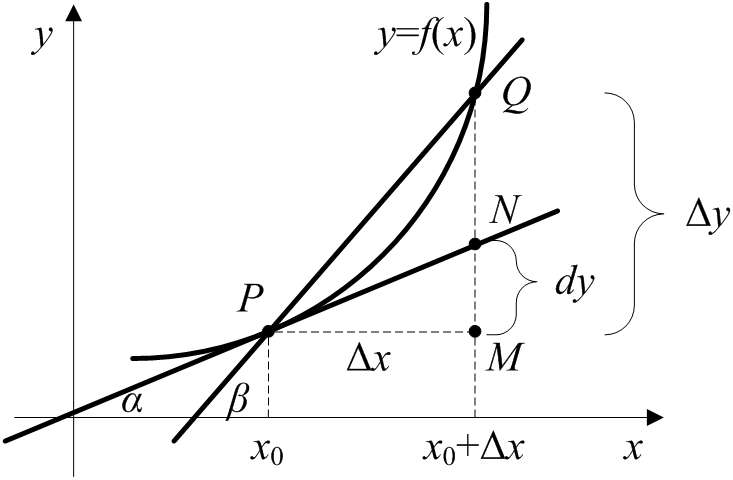
\includegraphics[height=4cm]{2.3.png}
\end{figure}

当{\it Q}点无穷逼近{\it P}的时候,即$\beta \rightarrow \alpha $,可得:
\[
\underset{\Delta x\rightarrow 0}{\lim}\Delta y=\underset{\Delta x\rightarrow 0}{\lim}\left( \tan \beta \cdot \Delta x \right) =\tan \alpha \cdot \Delta x=dy
\]
从几何上看,当{\it Q}点无穷逼近{\it P}的时候,线段{\it MQ}的长度无穷逼近线段{\it MN}的长度。
或者说,我们可以用线段{\it MQ}代替线段{\it MN},且线段{\it NQ}是可以被忽略的。
被忽略的{\it NQ}就是那个高阶无穷小量$o\left( \Delta x \right) $。

微分的几何意义是在一个微小的局部,我们可以用直线函数近似代替曲线函数,即“以直代曲”。
这种局部线性化的思想广泛应用于自然科学和工程。

%============================================================
\subsection{微分的物理应用}

用微分我们可以近似计算一些工程值。
若已知$f\left( x_0 \right) $,如何快速求$f\left( x_0+\Delta x \right) $处的值。
这类问题可以通过微分近似求解。当$\Delta x$足够小时,我们可以用$dy$代替$\Delta y$,从而有:
\[
y=f\left( x_0 \right) +\Delta y\approx f\left( x_0 \right) +dy
\]

~

\begin{example}
扩音器插头为一圆柱体,截面半径r=0.15cm,长l=4cm,为提高导电性,需要在该圆柱体侧面镀一层0.001cm的纯铜,问约需要多少。
\end{example}

解:

显然该问题就是估算体积的变化。
圆柱体体积:
\[
V=\pi r^2l
\]
侧面镀一层纯铜,相当于半径变化。
所用铜的体积等于由于半径的微小变化引起的圆柱体体积的微增量。
\[
dV=2\pi rl=2\pi \cdot 0.15\cdot 4\cdot 0.001=0.00377\mathrm{cm}^3
\]






\newpage
\section{导数的应用}

导数是描述一个函数的变化率,所以通过导数我们可以分析一个函数的变化趋势、形态、走向,进而用多项式近似该函数。
微分中值定理解决前者,泰勒展开和麦克劳林公式解决后者。

本节要点:
\begin{itemize}
    \item 掌握各个定理。
\end{itemize}

%============================================================
\subsection{微分中值定理}

\begin{theorem}[费马定理]
设$f\left( x \right) $在点$x_0$处可导,若$x_0$处是$f\left( x \right) $的一个极值点,则$f'\left( x_0 \right) =0$。
\end{theorem}

\begin{theorem}[罗尔定理]
设$f\left( x \right) $在$\left[ a,b \right] $连续,在$\left( a,b \right) $可导,若$f\left( a \right) =f\left( b \right) $,则必有$\xi \in \left( a,b \right) $,使得$f'\left( \xi \right) =0$。
即两端相等的光滑曲线必有极值点。
\end{theorem}

\begin{theorem}[拉格朗日定理]
设$f\left( x \right) $在$\left[ a,b \right] $连续,在$\left( a,b \right) $可导,则必有$\xi \in \left( a,b \right) $,使得$f'\left( \xi \right) =\frac{f\left( b \right) -f\left( a \right)}{b-a}$。
即可作切线和割线平行。
\end{theorem}

\begin{theorem}[柯西定理]
设$f\left( x \right) $在$\left[ a,b \right] $连续,在$\left( a,b \right) $可导,若$g'\left( x_0 \right) \ne 0$,则必有$\xi \in \left( a,b \right) $,使得$\frac{f'\left( \xi \right)}{g'\left( \xi \right)}=\frac{f\left( b \right) -f\left( a \right)}{g\left( b \right) -g\left( a \right)}$。
\end{theorem}

微分中值定理建立了函数在考察区间内的变化形态。
这四个微分中值定理,前提都是要求可导,说明被考察对象都是光滑曲线。
而光滑,则直觉上必然会有这些定理描述的现象。
充分理解光滑的含义,这些定理也将是不证自明。

费马定理可用于求解区间内的最大值最小值问题。

罗尔定理可用于判断一个方程有无根,考察它的原函数在区间内连续可导,如果区间端点值相等,则必有根。

拉格朗日定理和后面的积分中值定理是对应关系,以不同的角度描述了一个事情,一个从微分角度,一个从积分角度。

柯西定理是拉格朗日定理的推广。

%============================================================
\subsection{洛必达法则}

\begin{theorem}[洛必达法则(L'Hopital's rule)]
若$f\left( x \right) ,g\left( x \right) $满足:
\begin{itemize}
    \item $\underset{x\rightarrow x_0}{\lim}f\left( x \right) =0,\underset{x\rightarrow x_0}{\lim}g\left( x \right) =0$;
    \item 在点$x_0$的去心邻域内$f'\left( x \right) ,g'\left( x \right) $均存在,且$g'\left( x \right) \ne 0$;
    \item $\underset{x\rightarrow x_0}{\lim}\frac{f'\left( x \right)}{g'\left( x \right)}$存在(或为$\infty $);
\end{itemize}
则有:
\[
\underset{x\rightarrow x_0}{\lim}\frac{f\left( x \right)}{g\left( x \right)}=\underset{x\rightarrow x_0}{\lim}\frac{f'\left( x \right)}{g'\left( x \right)}
\]
\end{theorem}

洛必达法则用于求解$\frac{0}{0}$和$\frac{\infty}{\infty}$之类的不定型极限。
注意,其他类型的极限不能用洛必达法则。






\newpage
\section{泰勒展开}

\begin{tcolorbox}
从逻辑概念的归属来讲,泰勒定理属于级数的范畴,应该和三角级数编排在一起。
而从三角级数到傅里叶变换需要一点多元函数积分的概念,所以泰勒展开会在级数部分详细介绍。
但如果把泰勒展开完全编排在最后,等学完所有的微积分内容(特别是多元函数微积分)再学级数,那对很多工程应用来说就学了一堆不需要的东西(电子电路就不需要多元函数微积分的概念),而且大大增加学习难度。
所以一般教材的编排将泰勒定理放在这里讲述。
\end{tcolorbox}

本节讨论导数一个很重要、很典型的应用——多项式展开。

本节要点:
\begin{itemize}
    \item 掌握泰勒展开的概念;
    \item 从线性代数角度理解泰勒展开;
    \item 掌握麦克劳林公式;
    \item 熟悉泰勒展开的工程使用。
\end{itemize}

%============================================================
\subsection{泰勒定理}

之前在讨论微分时,我们将任意可导函数$f\left( x_0 \right) $在$x_0$的一个微小局部用一个线性表达式$f\left( x \right) \approx f\left( x_0 \right) +f'\left( x_0 \right) \left( x-x_0 \right) $描述。
进一步地,我们希望在$x_0$附近找到一个关于$x$的多项式$P\left( x \right) $,能够表示$x\left( x \right) $,要求很简单:
\begin{itemize}
    \item $P\left( x \right) $和$x\left( x \right) $在$x_0$有相同的函数值和1~n阶导数;
    \item $P\left( x \right) $和$x\left( x \right) $的误差能定量描述。
\end{itemize}

~

\begin{theorem}[泰勒(Taylor)定理]
若$f\left( x \right) $在$x_0$处满足n阶可导,则$f\left( x \right) $可以展开成:
\begin{align*}
f\left( x \right) &=f\left( x_0 \right) +f'\left( x_0 \right) \left( x-x_0 \right) +\frac{f''\left( x_0 \right)}{2!}\left( x-x_0 \right) ^2+\cdots \\
&\quad +\frac{f^{\left( n \right)}\left( x_0 \right)}{n!}\left( x-x_0 \right) ^n+o\left( \left( x-x_0 \right) ^n \right) \\
&=\left[ \sum_{i=0}^n{\frac{f^{\left( i \right)}\left( x_0 \right)}{i!}\left( x-x_0 \right) ^i} \right] +o\left( \left( x-x_0 \right) ^n \right)
\end{align*}
其中$R\left( x \right) :=o\left( \left( x-x_0 \right) ^n \right) $称为{\bf 佩亚诺(G. Peano)型余项}。
\end{theorem}

当$n=1$时,泰勒展开就是一阶微分形式:
\begin{align*}
&\because f\left( x \right) =f\left( x_0 \right) +f'\left( x_0 \right) \left( x-x_0 \right) +o\left( x-x_0 \right) \\
&\therefore \Delta y=f\left( x \right) -f\left( x_0 \right) =f'\left( x_0 \right) \left( x-x_0 \right) +o\left( x-x_0 \right)
\end{align*}

\begin{theorem}[泰勒(Taylor)定理]
若$f\left( x \right) $在区间$D$上满足n+1阶可导,则$\forall x,x_0\in D$,至少存在$\xi \in \left[ x,x_0 \right] $或$\xi \in \left[ x_0,x \right] $,使得:
\begin{align*}
f\left( x \right) &=f\left( x_0 \right) +f'\left( x_0 \right) \left( x-x_0 \right) +\frac{f''\left( x_0 \right)}{2!}\left( x-x_0 \right) ^2+\cdots \\
&\quad +\frac{f^{\left( n \right)}\left( x_0 \right)}{n!}\left( x-x_0 \right) ^n+\frac{f^{\left( n+1 \right)}\left( \xi \right)}{\left( n+1 \right) !}\left( x-x_0 \right) ^{n+1} \\
&=\left[ \sum_{i=0}^n{\frac{f^{\left( i \right)}\left( x_0 \right)}{i!}\left( x-x_0 \right) ^i} \right] +\frac{f^{\left( n+1 \right)}\left( \xi \right)}{\left( n+1 \right) !}\left( x-x_0 \right) ^{n+1}
\end{align*}
其中$R_n\left( x \right) :=\frac{f^{\left( n+1 \right)}\left( \xi \right)}{\left( n+1 \right) !}\left( x-x_0 \right) ^{n+1}$称为{\bf 朗格兰日(Lagrange)型余项}。
\end{theorem}

泰勒定理告诉我们,任何n阶可导函数,都可以展开成一个二项式。
虽然两个都是泰勒定理,但第二个泰勒定理的要求更严格,好处是给出了余项的表达式,可以用来估算误差。
泰勒定理其实就是一个函数的幂级数展开。

%============================================================
\subsection{从线性代数看泰勒展开}

从线性代数角度看来,泰勒展开就将函数将基变换为多项式。
原来$f\left( x \right) $的基为实数集$D$,变换后为:
\[
B=\left[ \begin{array}{c}
	1\\
	\left( x-x_0 \right)\\
	\left( x-x_0 \right) ^2\\
	\vdots\\
	\left( x-x_0 \right) ^n\\
\end{array} \right]
\]
相应地坐标为:
\[
\left[ f \right] _B=\left[ \begin{array}{c}
	f\left( x_0 \right)\\
	f'\left( x_0 \right)\\
	\frac{f''\left( x_0 \right)}{2!}\\
	\vdots\\
	\frac{f^{\left( n \right)}\left( x_0 \right)}{n!}\\
\end{array} \right]
\]
于是函数可以描述为:
\[
f\left( x \right) =B^T\left[ f \right] _B+R_n\left( x \right)
\]

%============================================================
\subsection{麦克劳林公式}

\begin{definition}[n阶麦克劳林(Maclaurin)公式]
{\bf 麦克劳林公式}是函数在0点处的泰勒展开,取$x_0=0$,泰勒展开公式变为:
\begin{align*}
f\left( x \right) &=f\left( 0 \right) +f'\left( 0 \right) \cdot x+\frac{f''\left( 0 \right)}{2!}\cdot x^2+\cdots +\frac{f^{\left( n \right)}\left( 0 \right)}{n!}\cdot x^n+o\left( x \right) \\
&=\left[ \sum_{i=0}^n{\frac{f^{\left( i \right)}\left( 0 \right)}{i!}\cdot x^i} \right] +o\left( x \right)
\end{align*}
\end{definition}

~

几个常用函数的麦克劳林公式:
\begin{align*}
&\left( 1+x \right) ^a=1+ax+\frac{a\left( a-1 \right)}{2!}x^2+\cdots +\frac{a\left( a-1 \right) \cdots \left( a-n \right)}{n!}x^n+o\left( x \right) \\
&e^x=1+x+\frac{x^2}{2!}+\cdots +\frac{x^n}{n!}+o\left( x \right) \\
&\sin x=x-\frac{x^3}{3!}+\frac{x^5}{5!}-\cdots +\left( -1 \right) ^{m-1}\frac{x^{2m-1}}{\left( 2m-1 \right) !}+o\left( x \right) \\
&\cos x=1-\frac{x^2}{2!}+\frac{x^4}{4!}-\cdots +\left( -1 \right) ^m\frac{x^{2m}}{\left( 2m \right) !}+o\left( x \right)
\end{align*}

特别地,一般在工程中常用:
\begin{align*}
&\left( 1+x \right) ^a=1+ax \\
&e^x=1+x \\
&\sin x=x \\
&\cos x=1-\frac{x^2}{2!}
\end{align*}

麦克劳林公式常用于工程上的公式推导,通过麦克劳林公式将超越方程简化成一次或二次方程,进而求解解析式。
如求解方程$e^x=\cos x-1$,在0附近可以用方程$1+x=-x^2/2!$代替求解。

%============================================================
\subsection{泰勒展开的工程意义}

要估算一个复杂的函数,通常的做法是用另一个简单的函数代替,即“化繁为简”。
这种方法(或思想)称为级数。
代替的函数必须简单,最好是初等函数的组合。
数学上有三种可行的初等函数代替展开:
\begin{itemize}
    \item 幂函数;
    \item 三角函数;
    \item 指数函数。
\end{itemize}
但由于欧拉公式,所以实际只剩下幂函数和三角函数两种方法。

幂函数展开的方法之一就是泰勒展开,三角函数展开就是傅里叶级数。
泰勒展开由于采用幂函数将超越方程化为二次方程,所以多用于手解超越方程或判断两个超越方程的大小关系。
傅里叶级数采用三角函数,使得原函数由一系列不同角频的正弦函数组成,所以通常用于考察一个函数的特征。






\newpage
\section{函数的性状}

本节我们用导数这个数学工具考察函数的性状。

本节要点:
\begin{itemize}
    \item 掌握函数单调性的判断;
    \item 掌握函数极值的判断;
    \item 掌握目标函数的优化步骤;
    \item 了解凸函数的概念;
    \item 了解琴声Jensen不等式和渐近线。
\end{itemize}

%============================================================
\subsection{单调性}

\begin{theorem}
若$f\left( x \right) \in D\left( a,b \right) $,则:
\begin{itemize}
    \item $f'\left( x \right) \geqslant 0\left( \leqslant 0 \right) \Leftrightarrow f\left( x \right) $在$\left( a,b \right) $上单调增(减);
    \item $f'\left( x \right) >0\left( <0 \right) \Leftrightarrow f\left( x \right) $在$\left( a,b \right) $上严格单调增(减)。
\end{itemize}
\end{theorem}

\begin{corollary}
若$f\left( x \right) \in C\left[ x_0,x \right] \cap D\left( x_0,x \right) $,且$f\left( x_0 \right) =0$,则:
\begin{itemize}
    \item 当$x>x_0$时$f'\left( x \right) >0$,则$f\left( x \right) >0$;
    \item 当$x>x_0$时$f'\left( x \right) <0$,则$f\left( x \right) <0$。
\end{itemize}
\end{corollary}

推论要表达的是当我们知道函数的某个起点和趋势,我们就可以判断函数的在该点后的值域。

%============================================================
\subsection{极值的判断}

微分中值定理中我们初步讨论了极值,这里给出具体的定义和详细讨论。

\begin{definition}[极值和极值点]
设函数$f\left( x \right) $在区间$D$上有定义,若$x_0\in D$存在邻域$N\left( x_0,\delta \right) \subseteq D$,使得$\forall x\in N$有:
\[
f\left( x \right) <f\left( x_0 \right) \quad \text{或} \quad f\left( x \right) >f\left( x_0 \right)
\]
则称$f\left( x_0 \right) $为$f\left( x \right) $在邻域$N$上的一个{\bf 极大值}(或{\bf 极小值},统称为{\bf 极值}),而点$x_0$称为$f\left( x \right) $在邻域$N$上的{\bf 极大值点}(或{\bf 极小值点},统称为{\bf 极值点})。
如果$f\left( x \right) $在区间$D$上可导,则极值点$x_0$处必有$f'\left( x_0 \right) =0$,但$f'\left( x_0 \right) =0$并不代表$x_0$为极值点,我们称$f'\left( x_0 \right) =0$时的$x_0$为$f\left( x_0 \right) =0$的{\bf 驻点}。
如果$f\left( x_0 \right) =0$在$x_0$处不可导,则$x_0$也有可能是极值点。
\end{definition}

\begin{theorem} \label{th_2_6_1}
设$f\left( x \right) =0$在点$x_0$处连续,在$N\left( \hat{x}_0,\delta \right) $内可导,则:
\begin{itemize}
    \item 若$\forall x\in \left( x_0-\delta ,x_0 \right) $有$f'\left( x \right) <0$,$\forall x\in \left( x_0,x_0+\delta \right) $有$f'\left( x \right) >0$,则$f\left( x_0 \right) $为极小值;
    \item 若$\forall x\in \left( x_0-\delta ,x_0 \right) $有$f'\left( x \right) >0$,$\forall x\in \left( x_0,x_0+\delta \right) $有$f'\left( x \right) <0$,则$f\left( x_0 \right) $为极大值;
    \item 若$\forall x\in N\left( \hat{x}_0,\delta \right) $有$f'\left( x \right) $恒为正或恒为负,$f\left( x_0 \right) $为非极值。
\end{itemize}
\end{theorem}

\begin{theorem} \label{th_2_6_2}
设$f\left( x \right) =0$在点$x_0$处存在二阶导数,且$f'\left( x \right) =0$,则:
\begin{itemize}
    \item 若$f''\left( x \right) >0$,则$f\left( x_0 \right) $为极小值;
    \item 若$f''\left( x \right) <0$,则$f\left( x_0 \right) $为极大值;
    \item 若$f''\left( x \right) =0$,不能判定。
\end{itemize}
\end{theorem}

\begin{theorem} \label{th_2_6_3}
设$f\left( x \right) =0$在点$x_0$处存在二阶及以上导数,且
\begin{align*}
&f'\left( x_0 \right) =f''\left( x_0 \right) =\cdots =f^{\left( n-1 \right)}\left( x_0 \right) =0 \\
&f^{\left( n \right)}\left( x_0 \right) \ne 0
\end{align*}
则:
\begin{itemize}
    \item $n$为偶数时,若$f^{\left( n \right)}\left( x_0 \right) >0$则$f\left( x_0 \right) $为极小值,若$f^{\left( n \right)}\left( x_0 \right) <0$则$f\left( x_0 \right) $为极大值;
    \item $n$为奇数时,$f\left( x_0 \right) $非极值。
\end{itemize}
\end{theorem}

上述3个定理是对微分中值定理中的费马定理的推广,费马定理给出的是极值点的必要条件,这里给出了极值的充要条件。
但必须注意,这些定理的前提是可导,不可导点也是潜在的极值点,需要判断。

定理\ref{th_2_6_1}可以从几何上理解,通过描述一阶导数的走势判断极值。
定理\ref{th_2_6_2}通过二阶导数定量化地描述了函数走势,定理证明采用泰勒展开,具体参见“教材\cite{book1}”。
定理\ref{th_2_6_3}是定理\ref{th_2_6_2}的推广。

%============================================================
\subsection{目标函数优化}

极值是一个小范围内的最值,如果将考察区域扩大,则对极值的考察就扩展为对最值的考察。
最值点将会出现在极值点、不可导点和边界点上。
工程上有很多类似考察最值的问题,数学上归结为{\bf 求解目标函数的最值问题},有时又称为{\bf 目标函数的最优化}。

若$f\left( x \right) $在$\left[ a,b \right] $内连续,$\left( a,b \right) $内存在有限个不可导点,则首先根据连续函数的性质,必然存在最值,且两个端点$a,b$、驻点和不可导点$x_i$都是最值可能的点,将这些点的函数值计算就可以判断最值,或者根据一阶导数判断最值。

~

\begin{example}
若$f\left( x \right) =\sqrt[3]{\left( x^2-2x \right) ^2}$,求$\left[ 0,3 \right] $上的最值。
\end{example}

解:

易得$f\left( x \right) $连续,考察一阶导数:
\[
f'\left( x \right) =\frac{4}{3}\frac{x-1}{\sqrt[3]{x^2-2x}}
\]
有$x=1$为驻点,$x=2$为不可导点,于是端点、驻点、不可导点集合:
\[
\left\{ 0,3,1,2 \right\}
\]
分别求解:
\[
f\left( 0 \right) =0 \quad f\left( 3 \right) =\sqrt[3]{9} \quad f\left( 1 \right) =1 \quad f\left( 2 \right) =0
\]
于是可得最值:
\[
f_{\min}=0 \quad f_{\max}=\sqrt[3]{9}
\]

~

\begin{example}
若要做一个容积为$V_0$的圆柱形储罐,怎样设计用料最省。
\end{example}

解:

圆柱形储罐容积$V=\pi r^2h$,用料为表面积:
\[
S\left( r \right) =2\pi r^2+2\pi rh=2\pi r^2+2\pi r\frac{V}{\pi r^2}=2\pi r^2+2\frac{V_0}{r},    r\in \left( 0,+\infty \right)
\]
即求$S\left( r \right) $的最值,考察一阶导数:
\[
S'\left( r \right) =4\pi r-2V_0\frac{1}{r^2}=\frac{4\pi r^3-2V_0}{r^2}
\]
在$\left( 0,+\infty \right) $上可导且只有一个驻点
\begin{align*}
&\because \frac{4\pi r^3-2V_0}{r^2}=0 \\
&\therefore r_0=\sqrt[3]{\frac{V_0}{2\pi}}
\end{align*}
考察二阶导数$S''\left( r \right) =\frac{4\pi r^3+4V_0}{r^3}>0$,所以该驻点为极小值点。
由于$S\left( r \right) $在$\left( 0,+\infty \right) $上只有一个极小值点,且无不可导点,无端点,所以$r_0$为$S\left( r \right) $的最小值点,此时:
\[
h_0=\frac{V_0}{\pi {r_0}^2}=2\sqrt[3]{\frac{V_0}{2\pi}}=2r_0
\]
即储罐高和底面直径相等时,用料最少。

~

\begin{example}
假设一个物理试验中,一共进行了$n$次测量,得到$x_1,x_2,\cdots ,x_n$,若用$\bar{x}$表示测量结果,问$\bar{x}$为多少使得测量的总平方误差
\[
TSE\left( \bar{x} \right) =\sum_{i=1}^n{\left( \bar{x}-x_i \right) ^2}
\]
最小。
\end{example}

解:

首先易得$TSE\left( x \right) $在$\left( -\infty ,+\infty \right) $连续,考察一阶和二阶导数:
\begin{align*}
&TSE'\left( x \right) =2\sum_{i=1}^n{\left( x-x_i \right)}=2nx-2\sum_{i=1}^n{x_i} \\
&TSE''\left( x \right) =2n>0
\end{align*}
可得,当
\[
\bar{x}=\frac{1}{n}\sum_{i=1}^n{x_i}
\]
时,$TSE\left( x \right) $有极小值,且是最小值。

这里可以看出,当取算术平均值时,总平方误差最小。
所以用算术平均值代替测量值,在总平方误差的角度是最可靠的。

%============================================================
\subsection{凸函数和拐点}

\begin{definition}[凸函数]
设$f\left( x \right) \in C\left[ a,b \right] $,若$\forall x_1,x_2\in \left( a,b \right) ,x_1\ne x_2$和$\forall t_1,t_2>0,t_1+t_2=1$:
\begin{itemize}
    \item 若$f\left( t_1x_1+t_2x_2 \right) <t_1f\left( x_1 \right) +t_2f\left( x_2 \right) $,则称$f\left( x \right) $在$\left( a,b \right) $上{\bf 下凸};
    \item 若$f\left( t_1x_1+t_2x_2 \right) >t_1f\left( x_1 \right) +t_2f\left( x_2 \right) $,则称$f\left( x \right) $在$\left( a,b \right) $上{\bf 上凸};
\end{itemize}
通常我们将下凸函数称为{\bf 凸函数}。
\end{definition}

\begin{theorem}
若$f\left( x \right) $在$\left[ a,b \right] $内连续,$\left( a,b \right) $内二阶可导且恒有$f''\left( x \right) >0$(或$f''\left( x \right) <0$),则$f\left( x \right) $在$\left( a,b \right) $内下凸(或上凸)。
\end{theorem}

\begin{proof}
略,依然使用泰勒展开。
\end{proof}

几何上,凸函数表示$\left[ a,b \right] $上任取两点作连线,$f\left( x \right) $都在连线之下。
注意这里取点的任意性。

\begin{definition}[拐点]
设$f\left( x \right) $在$N\left( x_0 \right) $内连续,若在$x_0$的左右两侧凸性相反,则称$x_0$为$f\left( x \right) $的{\bf 拐点}。
\end{definition}

\begin{theorem}
若$f\left( x \right) $在$\left( a,b \right) $内二阶可导,$x_0\in \left( a,b \right) $:
\begin{itemize}
    \item 若$x_0$是$f\left( x \right) $的一个拐点,则有$f''\left( x_0 \right) =0$;
    \item 若$f''\left( x_0 \right) =0$且$f''\left( {x_0}^+ \right) \cdot f''\left( {x_0}^- \right) <0$(即$x_0$两侧$f''\left( x \right) $异号),则$x_0$是$f\left( x \right) $的一个拐点。
\end{itemize}
\end{theorem}

%============================================================
\subsection{琴生(Jensen)不等式}

\begin{tcolorbox}
反过来我们用凸函数的定义可以获得一个比较重要的不等式。
\end{tcolorbox}

\begin{definition}[琴生(Jensen)不等式]
若$f\left( x \right) $在$\left( a,b \right) $内下凸,则对于
\begin{align*}
&\forall x_1,x_2,\cdots ,x_n\in \left( a,b \right) \\
&\forall t_1,t_2,\cdots ,t_n>0 \\
&\sum_{i=1}^n{t_i}=1
\end{align*}
必有:
\[
f\left( \sum_{i=1}^n{t_ix_i} \right) <\sum_{i=1}^n{\left[ t_if\left( x_i \right) \right]}
\]
其中$x_1,x_2,\cdots ,x_n$不全相等。
特别的,当$t_1=t_2=\cdots =t_n=1/n$时,有:
\[
f\left( \frac{x_1+x_2+\cdots +x_n}{n} \right) <\frac{f\left( x_1 \right) +f\left( x_2 \right) +\cdots +f\left( x_n \right)}{n}
\]
\end{definition}

%============================================================
\subsection{渐近线}

\begin{definition}[函数的渐近线]
对于曲线$f\left( x \right) $,若存在直线$y=kx+b$使得:
\[
\underset{x\rightarrow +\infty}{\lim}\left[ f\left( x \right) -y\left( x \right) \right] =0 \quad \text{或} \quad \underset{x\rightarrow -\infty}{\lim}\left[ f\left( x \right) -y\left( x \right) \right] =0
\]
则称$y=kx+b$为{\bf $f\left( x \right) $的渐近线},特别的当$k=0$时,称$y=b$为{\bf $f\left( x \right) $的水平渐近线}。
若曲线$f\left( x \right) $有:
\[
\underset{x\rightarrow {x_0}^-}{\lim}f\left( x \right) =\infty  \quad \text{或} \quad \underset{x\rightarrow {x_0}^+}{\lim}f\left( x \right) =\infty
\]
则称$x=x_0$为{\bf $f\left( x \right) $的垂直渐近线}。
\end{definition}

渐近线判断方法:
\begin{enumerate}
    \item 考察$\left( -\infty ,+\infty \right) $上未定义点$x_0$处的极限$\underset{x\rightarrow x_0}{\lim}f\left( x \right) $,若为$\infty $,说明有垂直渐近线$x=x_0$。
    \item 计算$k_1=\underset{x\rightarrow +\infty}{\lim}\frac{f\left( x \right)}{x}$、$k_2=\underset{x\rightarrow -\infty}{\lim}\frac{f\left( x \right)}{x}$,和$b_1=\underset{x\rightarrow +\infty}{\lim}\left[ f\left( x \right) -kx \right] $、$b_2=\underset{x\rightarrow -\infty}{\lim}\left[ f\left( x \right) -kx \right] $,获得斜渐近线或水平渐近线。
\end{enumerate}

~

\begin{example}
判断逻辑斯蒂(Logistic)函数$f\left( x \right) =\frac{c}{1+be^{-ax}}$的渐近线。
\end{example}

解:

$f\left( x \right) $在$\left( -\infty ,+\infty \right) $内均有定义,所以没有垂直渐近线,考察斜渐近线和水平渐近线:
\begin{align*}
&k_{1,2}=\underset{x\rightarrow \pm \infty}{\lim}\frac{f\left( x \right)}{x}=\underset{x\rightarrow \pm \infty}{\lim}\frac{c}{\left( 1+be^{-ax} \right) x}=0 \\
&b_1=\underset{x\rightarrow +\infty}{\lim}\left[ f\left( x \right) -kx \right] =\underset{x\rightarrow +\infty}{\lim}\frac{c}{1+be^{-ax}}=c \\
&b_2=\underset{x\rightarrow -\infty}{\lim}\left[ f\left( x \right) -kx \right] =\underset{x\rightarrow -\infty}{\lim}\frac{c}{1+be^{-ax}}=0
\end{align*}
可见$f\left( x \right) =\frac{c}{1+be^{-ax}}$有两条渐近线:
\begin{align*}
&y=c \\
&y=0
\end{align*}

~

\begin{example}
考察$f\left( x \right) =\frac{\left( x-3 \right) ^2}{4\left( x-1 \right)}$的渐近线。
\end{example}

解:

显然,$x=1$处未定义,考察:
\[
\underset{x\rightarrow 1}{\lim}\frac{\left( x-3 \right) ^2}{4\left( x-1 \right)}=\infty
\]
可得$x=1$为$f\left( x \right) $的一条垂直渐近线。
再考察斜渐近线和水平渐近线:
\begin{align*}
&k_{1,2}=\underset{x\rightarrow \pm \infty}{\lim}\frac{f\left( x \right)}{x}=\underset{x\rightarrow \pm \infty}{\lim}\frac{\left( x-3 \right) ^2}{4\left( x-1 \right) x}=\frac{1}{4} \\
&b_{1,2}=\underset{x\rightarrow \pm \infty}{\lim}\left[ f\left( x \right) -kx \right] =\underset{x\rightarrow \pm \infty}{\lim}\left[ \frac{\left( x-3 \right) ^2}{4\left( x-1 \right)}-\frac{x}{4} \right] =-\frac{5}{4}
\end{align*}
可得 只有一条斜渐近线:
\[
y=\frac{1}{4}x-\frac{5}{4}
\]






\newpage
\section{微分的应用}

本节以曲率为例讲解微分的应用。

%============================================================
\subsection{弧微分和曲率}

在工程技术中,要经常考虑曲线的弯曲程度,所谓曲线的“曲率”。

\begin{figure}[h]
\centering
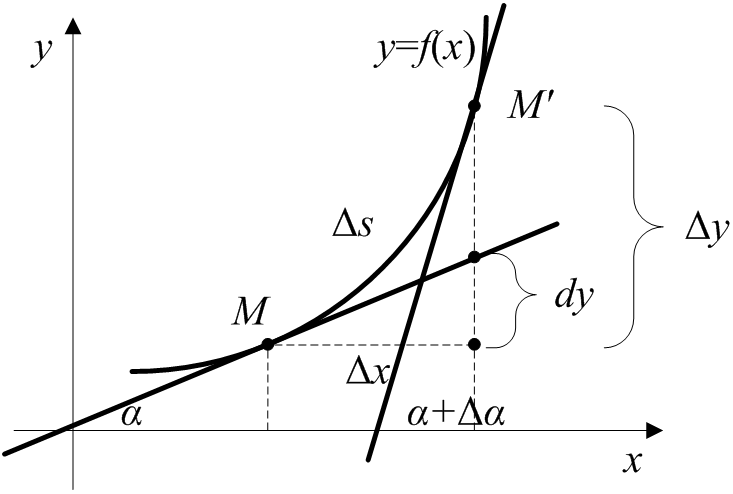
\includegraphics[height=4cm]{2.4.png}
\end{figure}

\begin{definition}[曲率]
我们定义曲线$y$上,切线转过的角度$\Delta \alpha $和弧长$\Delta s=\overset\frown{MM'}$的比值为{\bf 该弧段的平均曲率},记作$\bar{\kappa}$,即:
\[
\bar{\kappa}:=\frac{\Delta \alpha}{\Delta s}
\]
如果当$\Delta s\rightarrow 0$时$\bar{\kappa}$存在极限,就称该极限为{\bf 曲线$y$在点{\it M}处的曲率},记作$\kappa $,即:
\[
\kappa :=\underset{\Delta s\rightarrow 0}{\lim}\bar{\kappa}=\underset{\Delta s\rightarrow 0}{\lim}\frac{\Delta \alpha}{\Delta s}=\frac{d\alpha}{ds}
\]
\end{definition}

首先求解$d\alpha $:
\begin{align*}
&\because \frac{dy}{dx}=\tan \alpha \\
&\therefore \frac{d^2y}{dx^2}=\frac{d}{dx}\left( \tan \alpha \right) =\sec ^2\alpha \cdot \frac{d\alpha}{dx} \\
&\therefore d\alpha =\frac{d^2y}{dx^2}\cdot \frac{dx}{\sec ^2\alpha}=\frac{d^2y}{dx^2}\cdot \frac{dx}{1+\tan ^2\alpha}=\frac{d^2y}{dx^2}\cdot \frac{1}{1+\left( \frac{dy}{dx} \right) ^2}\cdot dx
\end{align*}
再求解$ds$(称为{\bf 弧微分}):
\[
ds=\sqrt{\left( dx \right) ^2+\left( dy \right) ^2}=\sqrt{1+\left( \frac{dy}{dx} \right) ^2}\cdot dx
\]
结合上述两式,得到曲率公式:
\[
\kappa =\underset{\Delta s\rightarrow 0}{\lim}\bar{\kappa}=\underset{\Delta s\rightarrow 0}{\lim}\frac{\Delta \alpha}{\Delta s}=\frac{d\alpha}{ds}=\frac{\frac{d^2y}{dx^2}\cdot \frac{1}{1+\left( \frac{dy}{dx} \right) ^2}\cdot dx}{\sqrt{1+\left( \frac{dy}{dx} \right) ^2}\cdot dx}=\frac{d^2y}{dx^2}\cdot \frac{1}{\left[ 1+\left( \frac{dy}{dx} \right) ^2 \right] ^{3/2}}
\]

\begin{tcolorbox}
曲率有正有负,表示凸还是凹。
其次,弧微分这个概念在微积分中会频繁出现,特别是在多元函数微积分中。
\end{tcolorbox}






\newpage
\section{本章小结}

形而下来讲,本章引入了微积分里的灵魂概念——导数。
如果将微积分定位为工程上的数学工具,则导数是这个工具中的数学基础,微分是作为数学的导数的第一个工程应用,如何用一个微小量代替全部量。
形而上来讲,本章解决了光滑的第二个要求。
至此,光滑的好函数——不断不折——在数学上有了严格的定义。

我们要将“光滑”这个概念作为微积分的出发点和落脚点,深入理解极限、连续、导数、微分这些概念。
我们喜欢的是光滑曲线,我们要考察的是光滑曲线,我们要寻找使用的也是光滑曲线。
所以我们首先定义光滑——不断不折。
通过连续定义什么是不断,通过可导定义什么是不折。
接着,我们考察光滑曲线的特征。
光滑的特征体现在连续上是最值、有界、介值三个定理。
由于可导等价于可微,所以不折的特征体现在可导上是微分中值定理,特别是拉格朗日定理。
充分领悟光滑这个概念,这些定理将会是无比自然。
最后,我们从“微”的角度考察光滑的好处,即光滑的实际价值。
我们提出了微分的概念,用一个线性小量代替绝对差量,当然,这得首先要求是光滑的。

至此,我们解决了光滑的问题,讨论了光滑在“微”方面的意义。
下一章积分,我们要讨论光滑在“累积”方面有哪些特征,可以帮助我们解决什么问题。






\newpage
\section{习题}

\begin{exercise}
求曲线$y=\cos x$在点$\left( \frac{\pi}{3},\frac{1}{2} \right) $处的切线和法线方程。
\end{exercise}

解:

使用曲线的切线和法线的公式即可。
\begin{align*}
&y=f'\left( x_0 \right) x+\left[ f\left( x_0 \right) -f'\left( x_0 \right) x_0 \right] \\
&y=-\frac{1}{f'\left( x_0 \right)}x+\left[ f\left( x_0 \right) +\frac{1}{f'\left( x_0 \right)}x_0 \right]
\end{align*}
得到切线和法线方程:
\begin{align*}
&\because f'\left( \frac{\pi}{3} \right) =-\sin \left( \frac{\pi}{3} \right) =-\frac{\sqrt{3}}{2} \\
&\therefore \begin{cases}
	y=-\frac{\sqrt{3}}{2}x+\left( \frac{1}{2}+\frac{\sqrt{3}}{2}\frac{\pi}{3} \right)\\
	y=\frac{1}{\frac{\sqrt{3}}{2}}x+\left( \frac{1}{2}+\frac{1}{-\frac{\sqrt{3}}{2}}\frac{\pi}{3} \right) =\frac{2}{\sqrt{3}}x+\left( \frac{1}{2}-\frac{2}{\sqrt{3}}\frac{\pi}{3} \right)\\
\end{cases}
\end{align*}

~

\begin{exercise}
求曲线$e^{xy}-2x-y=3$上点$\left( -1,0 \right) $所对应的切线方程。
\end{exercise}

解:

大体思路一样,只是需要用到隐函数求导:
\begin{align*}
&\because \frac{dy}{dx}=-\frac{F_x}{F_y}=-\frac{ye^{xy}-2}{xe^{xy}-1} \\
&\therefore f'\left( x_0 \right) =-\frac{-2}{-1-1}=-1 \\
&\therefore y=f'\left( x_0 \right) x+\left[ f\left( x_0 \right) -f'\left( x_0 \right) x_0 \right] =-x-1
\end{align*}

~

\begin{exercise}
求过点$\left( 3,0 \right) $与曲线$y=x^2$相切的直线方程。
\end{exercise}

解:

注意点$\left( 3,0 \right) $并不是曲线上的点,而是切线过的点。
假设切线切与点$x_0$,易得切线方程:
\[
y=2x_0\cdot x+\left( {x_0}^2-2x_0x_0 \right) =2x_0\cdot x-{x_0}^2
\]
带入点$\left( 3,0 \right) $求得$x_0$:
\begin{align*}
&\because 0=6x_0-{x_0}^2 \\
&\therefore x_0=0\,\,\mathrm{or}\,\,6
\end{align*}
于是得到2条切线:
\begin{align*}
&y=0 \\
&y=12x-36
\end{align*}

~

\begin{exercise}
在抛物线$y=1-x^2$上求两点,使得过这两点的切线与{\it x}轴形成一个等边三角形。
\end{exercise}

解:

首先假设切点为$x_0$,获得切线方程:
\[
y=\left( -2x_0 \right) x+\left[ \left( 1-{x_0}^2 \right) -\left( -2x_0 \right) x_0 \right] =\left( -2x_0 \right) x+\left( 1+{x_0}^2 \right)
\]
若与{\it x}轴形成等边三角形,则这两条直线的斜率必为$\pm \sqrt{3}$,于是:
\begin{align*}
&\because -2x_0=\pm \sqrt{3}\Rightarrow x_0=\pm \frac{\sqrt{3}}{2} \\
&\therefore \left( \pm \frac{\sqrt{3}}{2},\frac{1}{4} \right)
\end{align*}

~

\begin{exercise}
求和$y=x^2,y=-x^2+6x-5$两条曲线都相切的直线方程。
\end{exercise}

解:

假设和两条曲线分别切于点$x_1,x_2$,分别根据两条曲线易得切线:
\begin{align*}
y&=2x_1x+\left( {x_1}^2-2x_1x_1 \right) =2x_1x-{x_1}^2 \\
y&=\left( -2x_2+6 \right) x+\left[ \left( -{x_2}^2+6x_2-5 \right) -\left( -2x_2+6 \right) x_2 \right] \\
&=\left( -2x_2+6 \right) x+\left( {x_2}^2-5 \right)
\end{align*}
由于这两条切线是同一条,于是可以得到:
\[
\begin{cases}
	2x_1=-2x_2+6\\
	-{x_1}^2={x_2}^2-5\\
\end{cases}\Rightarrow \begin{cases}
	x_1=1\\
	x_2=2\\
\end{cases} \quad \mathrm{or} \quad \begin{cases}
	x_1=2\\
	x_2=1\\
\end{cases}
\]
即有两条切线都可以和$y=x^2,y=-x^2+6x-5$相切:
\begin{align*}
&y=2x-1 \\
&y=4x-4
\end{align*}

~

\begin{exercise}
给定椭圆$4x^2+y^2=5$,求与此椭圆相切于$\left( \pm 1,-1 \right) $的抛物线方程。
\end{exercise}

解:

椭圆和抛物线相切,则必有一切线,同时切于这两个曲线。
先求和椭圆的切于$\left( \pm 1,-1 \right) $的切线方程,椭圆方程的隐函数为$F=4x^2+y^2-5$,则切线:
\begin{align*}
&\because y'\left( x_0 \right) =-\frac{F_x}{F_y}=-\frac{8x_0}{2y_0} \\
&\therefore y=f'\left( x_0 \right) x+\left[ f\left( x_0 \right) -f'\left( x_0 \right) x_0 \right] =-\frac{8x_0}{2y_0}x+\left[ y_0+\frac{8x_0}{2y_0}x_0 \right] \\
&\therefore \begin{cases}
	y=-\frac{8x_0}{2y_0}x+\left[ y_0+\frac{8x_0}{2y_0}x_0 \right] =4x-5\\
	y=-\frac{8x_0}{2y_0}x+\left[ y_0+\frac{8x_0}{2y_0}x_0 \right] =-4x-5\\
\end{cases}
\end{align*}
假设抛物线方程$y=ax^2+bx+c$,则有切线:
\begin{align*}
&\because y'\left( x_0 \right) =2ax_0+b \\
&\therefore y=f'\left( x_0 \right) x+\left[ f\left( x_0 \right) -f'\left( x_0 \right) x_0 \right] =\left( 2ax_0+b \right) x+\left[ y_0-\left( 2ax_0+b \right) x_0 \right] \\
&\therefore \left\{ \begin{aligned}
	y&=\left( 2ax_0+b \right) x+\left[ y_0-\left( 2ax_0+b \right) x_0 \right]\\
	&=\left( 2a+b \right) x+\left[ -1-\left( 2a+b \right) \right]\\
	y&=\left( 2ax_0+b \right) x+\left[ y_0-\left( 2ax_0+b \right) x_0 \right]\\
	&=\left( -2a+b \right) x+\left[ -1+\left( -2a+b \right) x_0 \right]\\
\end{aligned} \right.
\end{align*}
于是得到:
\[
\begin{cases}
	2a+b=4\\
	-1-\left( 2a+b \right) =-5\\
	-2a+b=-4\\
	-1+\left( -2a+b \right) =-5\\
\end{cases}
\]
解得$a=2,b=0$后得到抛物线方程$y=2x^2+c$,再将$\left( \pm 1,-1 \right) $代入求得$c=-3$,于是最终得到抛物线方程:
\[
y=2x^2-3
\]

~

\begin{exercise}
若$f\left( x \right) $对任意实数$x_1,x_2$有$f\left( x_1+x_2 \right) =f\left( x_1 \right) f\left( x_2 \right) $,且$f'\left( 0 \right) =1$,证明$f'\left( x \right) =f\left( x \right) $。
\end{exercise}

解:

总体思路求解$f'\left( x \right) $。

首先我们可以根据$f\left( x_1+x_2 \right) =f\left( x_1 \right) f\left( x_2 \right) $得到:
\begin{align*}
&\because f\left( x_1+x_2 \right) =f\left( x_1 \right) f\left( x_2 \right) \\
&\therefore f\left( x \right) =f\left( 0 \right) f\left( x \right) \\
&\therefore f\left( 0 \right) =0\,\,\mathrm{or}\,\,1
\end{align*}
其次,将$f\left( x_1+x_2 \right) =f\left( x_1 \right) f\left( x_2 \right) $两边求导得到:
\begin{align*}
&\because f'\left( x_1+x_2 \right) =\left[ f\left( x_1 \right) f\left( x_2 \right) \right] '=f'\left( x_1 \right) f\left( x_2 \right) +f\left( x_1 \right) f'\left( x_2 \right) \\
&\therefore f'\left( x \right) =f'\left( x+0 \right) =f'\left( x \right) f\left( 0 \right) +f\left( x \right) f'\left( 0 \right) =f'\left( x \right) f\left( 0 \right) +f\left( x \right)
\end{align*}
当$f\left( 0 \right) =0$时,有
\[
f'\left( x \right) =f'\left( x \right) f\left( 0 \right) +f\left( x \right) =f\left( x \right)
\]
当$f\left( 0 \right) =1$时,有
\[
f'\left( x \right) =f'\left( x \right) f\left( 0 \right) +f\left( x \right) =f'\left( x \right) +f\left( x \right)
\]
此时解得函数表达式为$f\left( x \right) =0$,也即$f'\left( x \right) =f\left( x \right) $,证毕。










\chapter{一元函数积分学}

物理问题中,有两类问题:1)求解一段非均匀物理量的累积;2)求解平均值。
积分用于解决这类问题。

本章先给出解决这类问题的方法——定积分。
由于从概念入手求解定积分过程繁琐,不具普遍性,所以随后通过微积分基本定理(牛顿莱布尼兹方程)引出不定积分,并讨论各种不定积分的求解方法,使得定积分的求解方法化。

对于定积分:
\begin{itemize}
    \item 充分理解定积分的概念、数学意义、几何意义和物理意义。
    \item 充分理解积分上限函数和原函数的概念。
    \item 掌握运用定积分求解工程问题(微元法)。
\end{itemize}

对于不定积分:
\begin{itemize}
    \item 理解不定积分的概念。
    \item 学会求解不定积分。
\end{itemize}

积分和微分是一个事物的两个方面,有着对立统一的矛盾关系。
学习积分要时时刻刻想着微分,对于积分中的每个概念和定理要思考在微分下的对应体。

\newpage
\section{一元函数积分学}

本节给出定积分的概念和意义。
定积分是一元函数积分学的目的,后续的牛顿莱布尼兹公式和不定积分是求解定积分的方法。

本节要点:
\begin{itemize}
    \item 理解定积分的概念和意义;
    \item 掌握用概念求解定积分。
\end{itemize}

%============================================================
\subsection{定积分的概念}

\begin{definition}[定积分]
设函数$f\left( x \right) $在$\left[ a,b \right] $上有界,将$\left[ a,b \right] $划分为$n$个小区间$a=x_0<x_1<x_2<...<x_{n-1}<x_n=b$,记每个小区间的长度$\Delta x_i=x_i-x_{i-1},i=1,2,...,n$,令最大长度$\lambda =\max \left\{ \Delta x_i \right\} $,在每个小区间$\left[ x_{i-1},x_i \right] $上任取一点$\xi _i\in \left[ x_{i-1},x_i \right] $,作和式$\sum_{i=1}^n{\left[ f\left( \xi _i \right) \cdot \Delta x_i \right]}$,若无论区间$\left[ a,b \right] $如何划分也无论点$\xi _i$如何选取,极限$\underset{\lambda \rightarrow 0}{\lim}\sum_{i=1}^n{\left[ f\left( \xi _i \right) \cdot \Delta x_i \right]}$存在且唯一,则称{\bf $f\left( x \right) $在$\left[ a,b \right] $上可积},该极限的值称为{\bf $f\left( x \right) $在$\left[ a,b \right] $上的定积分(definite integral)},记作$\int_a^b{f\left( x \right) dx}$,即:
\[
\int_a^b{f\left( x \right) dx}:=\underset{\lambda \rightarrow 0}{\lim}\sum_{i=1}^n{\left[ \xi _i\cdot \Delta x_i \right]}
\]
其中:
\begin{itemize}
    \item $x$:积分变量;
    \item $f\left( x \right) $:被积函数;
    \item $f\left( x \right) dx$:积分表达式,也称{\bf 微元};
    \item $a,b$:积分下限,积分上限;
    \item $\left[ a,b \right] $:积分区间。
\end{itemize}
\end{definition}

这个积分定义是黎曼(Riemann)给出的,通常称作{\bf 黎曼积分}。
黎曼积分存在的两个前提条件可以概括为闭区间和有限不连续。

\begin{tcolorbox}
黎曼可积的充要条件是勒贝格(Lebesgue)定理,即$f\left( x \right) $在$\left[ a,b \right] $上的不连续点组成的集合是一个零测度集。
如果不符合,则没有黎曼积分,需要扩充到勒贝格积分。
\end{tcolorbox}

注意,定积分概念里的两个“无关”:
\begin{itemize}
    \item 与区间划分方法无关,即$n$个小区间可以等分,也不可以不等分;
    \item 与区间点$\xi _i$的取法无关,即可以取在头、尾、中或者小区间内的任意一点。
\end{itemize}

\begin{tcolorbox}
一般的微积分教材里,将$\Delta x_i$称为“长度”。
但要特别注意,这个所谓的“长度”,是规定了方向的,是沿着{\it x}轴正方向,即$\Delta x_i=x_i-x_{i-1}$,不是$\Delta x_i=x_{i-1}-x_i$。
$\Delta x_i$必然是一个大于0的量。所以才有性质$\int_a^b{f\left( x \right) dx}=-\int_b^a{f\left( x \right) dx}$,细品!
\end{tcolorbox}

研究一函数在某一区间是否可积,关键在于判断和式极限
\[
\underset{\lambda \rightarrow 0}{\lim}\sum_{i=1}^n{\left[ f\left( \xi _i \right) \cdot \Delta x_i \right]}
\]
是否存在且唯一,步骤如下:
\begin{enumerate}
    \item 划分区间,通常等分;
    \item 取权重,通常取小区间的头或者尾;
    \item 求和式极限。
\end{enumerate}
所以定积分也是极限。
和求导一样,定积分也是对函数的一种运算,具体来说是对被积函数的一种运算,通过加权求和取极限这一过程得到另一个函数。
从集合角度,定积分是一个函数集合到另一个函数集合的映射。
这点在学习积分上限函数这个概念后细品!

%============================================================
\subsection{定积分的性质和定理}

区间性:
\begin{align*}
&a=b \quad \Rightarrow \quad \int_a^b{f\left( x \right) dx}=0 \\
&a\ne b \quad \Rightarrow \quad \int_a^b{f\left( x \right) dx}=-\int_b^a{f\left( x \right) dx}
\end{align*}

线性性:
\[
\int_a^b{\left[ mf\left( x \right) +ng\left( x \right) \right] dx}=m\int_a^b{f\left( x \right) dx}+n\int_a^b{g\left( x \right) dx}
\]

区间可加性:
\[
\int_a^b{f\left( x \right) dx}=\int_a^c{f\left( x \right) dx}+\int_c^b{f\left( x \right) dx}
\]

保号性:
\begin{align*}
&f\left( x \right) \geqslant 0 \quad \Rightarrow \quad \int_a^b{f\left( x \right) dx}\geqslant 0 \\
&f\left( x \right) \geqslant g\left( x \right) \quad \Rightarrow \quad \int_a^b{f\left( x \right) dx}\geqslant \int_a^b{g\left( x \right) dx}
\end{align*}

~

\begin{theorem}[连续可积定理]
$f\left( x \right) $在$\left[ a,b \right] $上连续$\Rightarrow f\left( x \right) $在$\left[ a,b \right] $上可积。
\end{theorem}

\begin{theorem}[有界可积定理]
$f\left( x \right) $在$\left[ a,b \right] $上有界,且只有有限个一类间断点$\Rightarrow f\left( x \right) $在$\left[ a,b \right] $上可积。
\end{theorem}

\begin{theorem}[估值定理]
设$M,m$分别是$f\left( x \right) $在$\left[ a,b \right] $上的最大值和最小值,则
\[
m\left( b-a \right) \leqslant \int_a^b{f\left( x \right) dx}\leqslant M\left( b-a \right)
\]
\end{theorem}

\begin{theorem}[积分中值定理]
若$f\left( x \right) $在$\left[ a,b \right] $上连续,则存在$\xi \in \left( a,b \right) $,使得
\[
\int_a^b{f\left( x \right) dx}=f\left( \xi \right) \left( b-a \right)
\]
\end{theorem}

估值定理和积分中值定理常用于定理的证明。
积分中值定理对应的微分中值定理中的拉格朗日定理,几何上表示必有矩形和曲边梯形面积相等,物理上必有均值点$\xi $及其均值$f\left( \xi \right) $。

\begin{tcolorbox}
细品后能发现,这些定理对曲线都要求不断。相比导数和微分,要求宽松了些。
\end{tcolorbox}

%============================================================
\subsection{定积分的代数意义}

在数学上,和式$\sum_{i=1}^n{\left[ f\left( \xi _i \right) \cdot \Delta x_i \right]}$可以看成加权和,每个累加项$\Delta x_i$加了权重$f\left( \xi _i \right) $后的代数和,整个和式也可以看成矩阵乘法:
\[
\sum_{i=1}^n{\left[ f\left( \xi _i \right) \cdot \Delta x_i \right]}=\left[ \begin{matrix}
	f\left( \xi _1 \right)&		f\left( \xi _2 \right)&		\cdots&		f\left( \xi _n \right)\\
\end{matrix} \right] \cdot \left[ \begin{array}{c}
	\Delta x_1\\
	\Delta x_2\\
	\vdots\\
	\Delta x_n\\
\end{array} \right]
\]
定积分就是当每个累加项都趋于无穷小,划分趋于无穷细、无穷多,情况下的这个代数和的极限。

\begin{tcolorbox}
从忽略高阶无穷小量的角度看,定积分的位置有点像微分。
\end{tcolorbox}

%============================================================
\subsection{定积分的几何意义}

考察曲线$y=f\left( x \right) $。
$f\left( \xi _i \right) \cdot \Delta x_i$是小区间的面积,和式$\sum_{i=1}^n{\left[ f\left( \xi _i \right) \cdot \Delta x_i \right]}$是所有小区间的面积的和,当小区间宽度越来越小时,和就越来越接近曲线下的面积。
当每个小区间的宽度都无穷小的时候,和式极限就是曲线下的面积。
所以几何上,定积分就是被积函数$y=f\left( x \right) $和{\it x}轴在积分区间$\left[ a,b \right] $里围成的面积。
\begin{figure}[h]
\centering
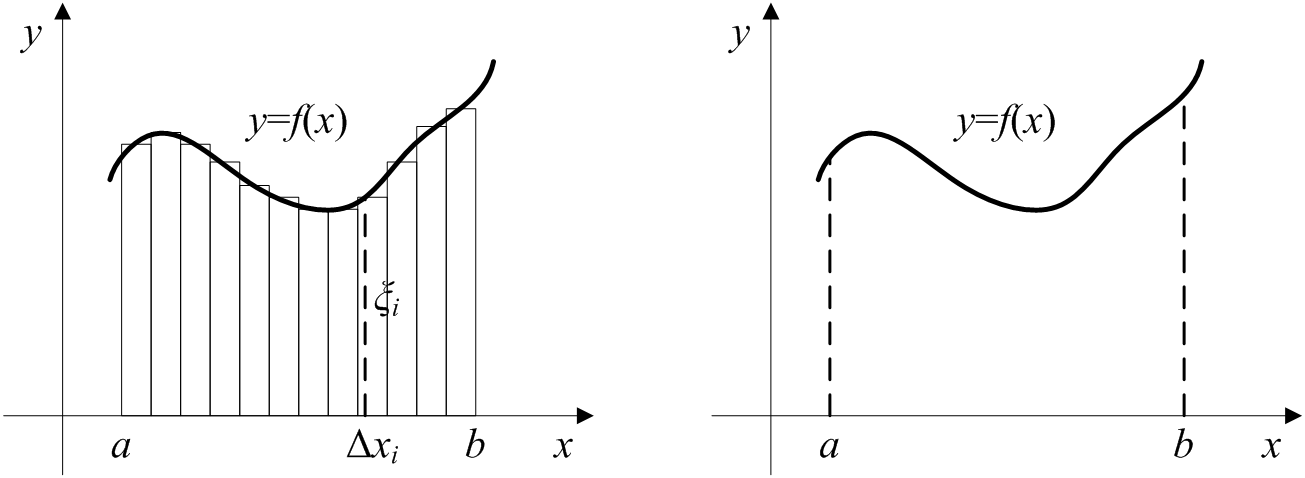
\includegraphics[height=3.5cm]{3.1.png}
\end{figure}

%============================================================
\subsection{定积分的物理意义}

物理量可以看成是很多分段小量的集合,每个小量又可以看成“加权小量”。
比方总路程$S$就可以看成很多分段$\Delta S$的累积,而$\Delta S$又是单位时间上平均速度的加权结果$\Delta S=\bar{v}\left( t \right) \cdot \Delta t$。
所以总路程为:
\[
S=\sum{\Delta S}=\sum{\left[ \bar{v}\left( t \right) \cdot \Delta t \right]}
\]
当单位时间$\Delta t\rightarrow 0$时,$\Delta t=dt$且有平均速度变成瞬时速度$\bar{v}\left( t \right) =v\left( t \right) $,有限段小路程变成无穷多段无穷小的路程$\Delta S=ds$,最终求和变成求积分:
\[
S=\int{ds}=\int{v\left( t \right) dt}
\]
这里需要注意的是,由于微元变量和变量本身有同样的量纲,所以$dt$的单位$t$和一样是秒,$ds=vdt$的单位是米。
% \begin{figure}[h]
% \centering
% 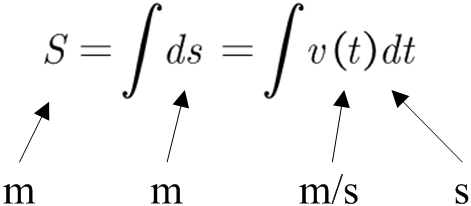
\includegraphics[height=2cm]{3.2.png}
% \end{figure}
所以,只要物理量是可以描述为加权积累效果的,都可以用定积分计算。






\newpage
\section{牛顿莱布尼兹公式}

上一节给出定积分的定义。
然而用定义求解定积分非常麻烦。
本节首先通过原函数的定义给出被积函数和导数运算之间的关系,然后介绍牛顿莱布尼兹公式,最后使用对被积函数求导逆运算求解定积分,大大简化了运算。

本节要点:
\begin{itemize}
    \item 掌握积分上限函数的概念;
    \item 掌握原函数的概念;
    \item 深入理解牛顿莱布尼兹公式。
\end{itemize}

%============================================================
\subsection{积分上限函数的概念}

\begin{definition}[积分上限函数]
如果对于区间$\left[ a,b \right] $上任意$x$,若存在定积分$\int_a^x{f\left( t \right) dt}$,则值必然唯一,且称它为{\bf $f\left( x \right) $在$\left[ a,b \right] $上的积分上限函数(accumulation function)},记为$F\left( x \right) $,即:
\[
F\left( x \right) :=\int_a^x{f\left( t \right) dt}
\]
\end{definition}

从几何上看,$F\left( x \right) $就是$f\left( x \right) $在$\left[ a,b \right] $上围成的面积,是自变量为$x$的函数,所以有时也称{\bf 面积函数}。

函数在给定区间的定积分是一个确定的数,而积分上限函数是对该函数的一种运算,得到的结果是另一个函数。
这点和导数和导函数类似。

%============================================================
\subsection{原函数的概念}

\begin{definition}[原函数]
若函数$f\left( x \right) $在$\left[ a,b \right] $上连续,则函数$F\left( x \right) $在$\left[ a,b \right] $上可导,且$F'\left( x \right) =f\left( x \right) $,称$F\left( x \right) $为{\bf $f\left( x \right) $在$\left[ a,b \right] $上的一个原函数}。
\end{definition}

\begin{proof}
即证明$F'\left( x \right) =f\left( x \right) $,从导数的定义出发,结合积分中值定理,有:
\begin{align*}
F'\left( x_0 \right) &=\underset{\Delta x\rightarrow 0}{\lim}\frac{\int_a^{x_0+\Delta x}{f\left( d \right) dt}-\int_a^{x_0}{f\left( d \right) dt}}{\Delta x} \\
&=\underset{\Delta x\rightarrow 0}{\lim}\frac{\int_{x_0}^{x_0+\Delta x}{f\left( d \right) dt}}{\Delta x}=\underset{\Delta x\rightarrow 0}{\lim}\frac{f\left( \xi \right) \cdot \Delta x}{\Delta x}
\end{align*}
当$\Delta x\rightarrow 0$时,有$\xi \rightarrow x_0$,从而:
\[
F'\left( x_0 \right) =\underset{\Delta x\rightarrow 0}{\lim}\frac{f\left( \xi \right) \cdot \Delta x}{\Delta x}=f\left( x_0 \right)
\]
\end{proof}

注意,“原函数”是“积分上限函数”的子集。
“积分上限函数”不要求被积函数连续,而“原函数”需要被积函数具备连续性。

$F\left( x \right) =\int_a^x{f\left( t \right) dt}$仅表示$f\left( x \right) $可积性。
如果$f\left( x \right) $不连续,那只要满足区间内有界,且一类间断点有限个,依然可积(即满足“有界可积定理”),只是$F\left( x \right) $在间断点是不可导的。
而一旦$f\left( x \right) $满足连续性要求,则除了满足上式,还满足$F'\left( x \right) =f\left( x \right) $,即整个$\left[ a,b \right] $上可导。

至此,对于连续函数$f\left( x \right) $,我们找到了计算定积分(数值计算)和函数求导(函数运算)之间的关系。
如果$F\left( x \right) $的导数正好是$f\left( x \right) $,则$F\left( x \right) $就是$f\left( x \right) $的定积分,即:
\begin{align*}
&\text{微分形式表达:} F'\left( x \right) =f\left( x \right) \\
&\text{积分形式表示:} F\left( x \right) =\int_a^x{f\left( t \right) dt}
\end{align*}

在积分定理中,原函数和被积函数唯一的联系是$x$,且$x$必然出现在积分上限(如果是积分下限,可以对调换到上限,如果同时出现在上下限,必须通过区间可加性定理拆分成上下限)。

%============================================================
\subsection{积分复合函数的求导}

\begin{definition}[积分复合函数]
当原函数的积分上限以函数的形式出现时,如:
\[
F\left( x \right) =\int_a^{\varphi \left( x \right)}{f\left( t \right) dt}
\]
称为{\bf 积分复合函数}。
对于此类函数,根据复合函数求导法则,有:
\[
F'\left( x \right) =\left[ \frac{d}{d\varphi}\int_a^{\varphi \left( x \right)}{f\left( t \right) dt} \right] \cdot \frac{d\varphi}{dx}=f\left[ \varphi \left( x \right) \right] \cdot \varphi '\left( x \right)
\]
\end{definition}

~

\begin{example}
已知$F\left( x \right) =\int_a^{x^2+1}{\sin \left( t+1 \right) dt}$,求$F'\left( x \right) $。
\end{example}

解:
\[
F'\left( x \right) =f\left[ \varphi \right] \cdot \varphi '=\sin \left[ \left( x^2+1 \right) +1 \right] \cdot \left( x^2+1 \right) '=2x\sin \left( x^2+2 \right)
\]

~

\begin{example}
求$\underset{x\rightarrow 0}{\lim}\frac{\int_{\cos x}^1{e^{-t^2}dt}}{x^2}$。
\end{example}

解:

可用洛必达法则求解:
\begin{align*}
&\because \left( \int_{\cos x}^1{e^{-t^2}dt} \right) '=f\left[ \varphi \right] \cdot \varphi '=-e^{-\cos ^2x}\cdot \left( -\sin x \right) =\sin x\cdot e^{-\cos ^2x} \\
&\therefore \underset{x\rightarrow 0}{\lim}\frac{\int_{\cos x}^1{e^{-t^2}dt}}{x^2}=\underset{x\rightarrow 0}{\lim}\frac{\sin x\cdot e^{-\cos ^2x}}{2x}=\frac{1}{2}\underset{x\rightarrow 0}{\lim}e^{-\cos ^2x}=\frac{1}{2e}
\end{align*}

%============================================================
\subsection{微积分基本定理}

\begin{theorem}[微积分基本定理]
如果$F\left( x \right) $是连续函数$f\left( x \right) $在$\left[ a,b \right] $上的一个原函数,即$F'\left( x \right) =f\left( x \right) $,则:
\[
\int_a^b{f\left( x \right) dx}=F\left( b \right) -F\left( a \right)
\]
该公式称为{\bf 牛顿—莱布尼兹(Newton-Leibniz)公式}。
\end{theorem}

牛顿莱布尼兹公式告诉我们,只要是连续函数,则在一个区域内的积分只跟其两端有关。
更抽象一点,对区域的考察可以变成对其边界的考察。
学完多元函数微积分(特别是统一公式)后,再回来细品牛顿莱布尼兹公式!

%============================================================
\subsection{再看定积分的几何意义}

假设函数$y=f\left( x \right) $在区间$\left[ a,b \right] $可导,已知$x$的变化量$\Delta x$,如何确定$\Delta y$。
首先,将区间$\left[ a,b \right] $化为$n$个小区间,运用微分的概念每个小区间可以认为有:
\[
dy=y'\cdot dx
\]
\begin{figure}[h]
\centering
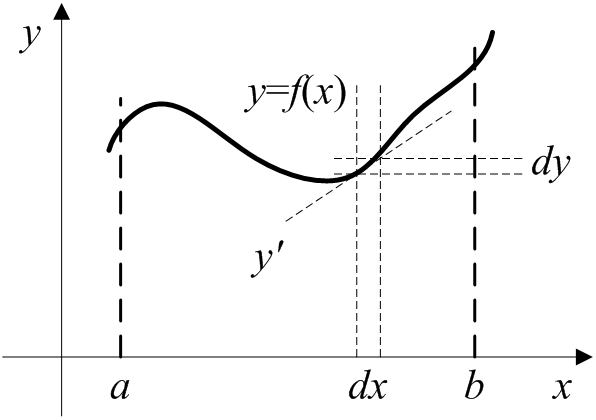
\includegraphics[height=3.5cm]{3.3.png}
\end{figure}

再将这些小区间上的微增量$dy$累积,就能得到$\Delta y$:
\[
\Delta y=\int_a^b{dy}=\int_a^b{y'\cdot dx}
\]
这里,对于每个小区间,$y'$可以认为是$dx$的权重,且$y'$有正有负。
几何上这个权重使得该段对$y$的变化量贡献也有正有负。
最终,$\Delta y$由各个$dy$累积得到。

%============================================================
\subsection{再看定积分的物理意义}

以变速运动为例。
从总体性考察,在一个范围内走过的路程$S\left( t \right) $为过程中的每个小微元$ds\left( t \right)$累积而成:
\[
S\left( t \right) =\int_0^t{ds\left( t \right)}
\]
从局部性考察,极端的时间内走过的路程和时间的比为一个固定的值:
\[
v\left( t \right) =\frac{ds\left( t \right)}{dt}
\]
结合上述两式:
\[
S\left( t \right) =\int_0^t{ds\left( t \right)}=\int_0^t{v\left( t \right) \cdot dt}
\]

\begin{tcolorbox}
“所谓的积分,就是由微分累积而成,所谓的微分,就是积分的局部化分析。”
这就是“教材\cite{book2}”中始终贯穿的微积分的矛盾统一论。
\end{tcolorbox}

%============================================================
\subsection{再看中值定理}

将微分中值定理(拉格朗日定理)和积分中值定义对比看。

用牛顿莱布尼兹公式,拉格朗日定理可以写为:
{\bf 设$F\left( x \right) $在$\left[ a,b \right] $连续,在$\left( a,b \right) $可导,则必有$\xi \in \left( a,b \right) $,使得$f\left( \xi \right) =F'\left( \xi \right) =\frac{F\left( b \right) -F\left( a \right)}{b-a}$。}

对比积分中值定理:
{\bf 若$f\left( x \right) $在$\left[ a,b \right] $上连续,则必有$\xi \in \left( a,b \right) $,使得$\int_a^b{f\left( x \right) dx}=f\left( \xi \right) \left( b-a \right)$。}

可见,两个中值定理描述的是一件事,只不过从两个方面描述而已。
这也反映出微分和积分是对立统一的。






\newpage
\section{半章小结}

至此,导数、微分、定积分三者关系确立:
\begin{itemize}
    \item 导数是整个微积分的基础;
    \item 微分定理给出了微增量和导数的关系$df\left( x \right) =f'\left( x \right) \cdot dx$;
    \item 牛顿莱布尼兹公式给出了累积量和导数的关系$\int_a^b{f\left( x \right) dx}=F\left( b \right) -F\left( a \right)$。
\end{itemize}

微分和积分所表达的是一个事物的两个方面,这个事物就是光滑。
微分是从“变化”的角度看光滑,积分是从“累积”的角度看光滑。
所以,一般地,微分里的概念和定理在积分里都会有对应的表达。
也正是微分和积分的这种对立统一关系,使得在解决实际问题时才有“微元法”这个普遍意义上的数学方法。

至此,微积分的基本思想建立完成。
我们需要从“微”和“积”两个方面理解微分和积分的对立,更要从逻辑论和认识论上理解微分和积分这一对矛盾体的对立统一。
这对矛盾体统一在光滑,是光滑衍生出来的在微和积方面的两个对立。






\newpage
\section{不定积分}

本节给出不定积分这个概念,这个概念完全是为了求解定积分,将定积分的求解过程中的求原函数步骤独立出来研究,讨论各种方法(换元法、凑微法、部分积分法等)。

本节要点:
\begin{itemize}
    \item 掌握不定积分的计算方法。
\end{itemize}

%============================================================
\subsection{不定积分的概念}

\begin{definition}[不定积分]
若某区间上$F\left( x \right) $是$f\left( x \right) $的一个原函数,则$f\left( x \right) $所有原函数的一般表达式$F\left( x \right) +C$称为{\bf $f\left( x \right) $的不定积分(indefinite function)},记为$\int{f\left( x \right) dx}$,即:
\[
\int{f\left( x \right) dx}:=F\left( x \right) +C
\]
其中:
\begin{itemize}
    \item $x$:积分变量;
    \item $f\left( x \right) $:被积函数;
    \item $f\left( x \right) dx$:积分表达式。
\end{itemize}
\end{definition}

定积分可以理解为不定积分在一段区间内的变化量。

%============================================================
\subsection{不定积分的几何意义}

\begin{figure}[h]
\centering
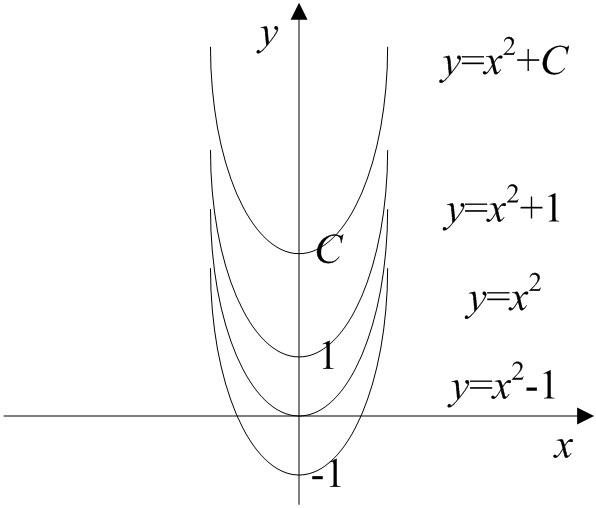
\includegraphics[height=4cm]{3.4.png}
\end{figure}

切线符合$y=x^2$的所有曲线的集合。

%============================================================
\subsection{不定积分的性质}

互逆运算:
\begin{align*}
&\left[ \int{f\left( x \right) dx} \right] '=f\left( x \right) \\
&\int{F'\left( x \right) dx}=F\left( x \right) +C
\end{align*}

线性性:
\[
\int{\left[ mf\left( x \right) +ng\left( x \right) \right] dx}=m\int{f\left( x \right) dx}+n\int{g\left( x \right) dx}
\]

\begin{tcolorbox}
线性性对应着导数运算中的$\left( f\pm g \right) '=f'\pm g'$。
\end{tcolorbox}

%============================================================
\subsection{不定积分计算方法}

{\bf 换元法(凑微分法)}:设$u=u\left( x \right) $具有连续导数,$F\left( u \right) $是$f\left( u \right) $的一个原函数,则:
\[
\int{f\left( u \right) u'\left( x \right) dx}=\int{f\left( u \right) du}=F\left( u \right) +C=F\left[ u\left( x \right) \right] +C
\]

\begin{tcolorbox}
线性性对应着导数运算中的$\frac{dy}{dx}=\frac{dy}{du}\cdot \frac{du}{dx}$。
\end{tcolorbox}

常用换元公式:
\begin{align*}
&\int{f\left( ax+b \right) dx}=\frac{1}{a}\int{f\left( ax+b \right) d\left( ax+b \right)} \quad a\ne 0 \\
&\int{f\left( x^a \right) x^{a-1}dx}=\frac{1}{a}\int{f\left( x^a \right) d\left( x^a \right)} \quad a\ne 0 \\
&\int{f\left( e^x \right) e^xdx}=\int{f\left( e^x \right) d\left( e^x \right)} \\
&\int{f\left( \ln x \right) \frac{1}{x}dx}=\int{f\left( \ln x \right) d\left( \ln x \right)} \\
&\int{\frac{\varphi '\left( x \right)}{\varphi \left( x \right)}dx}=\int{\frac{1}{\varphi \left( x \right)}d\varphi \left( x \right)}=\ln \left| \varphi \left( x \right) \right|+C
\end{align*}

~

{\bf 部分积分法}:设$u\left( x \right) ,v\left( x \right) $都具有连续导数,则:
\[
\int{uv'dx}=uv-\int{u'vdx} \quad \text{或写成} \quad \int{udv}=uv-\int{vdu}
\]

\begin{tcolorbox}
部分积分法和微分中的导数运算法则对应,$\left( fg \right) '=f'g+fg'$。
\end{tcolorbox}

%============================================================
\subsection{基本积分公式}

\begin{align*}
&\int{0dx}=C \\
&\int{x^adx}=\frac{1}{a+1}x^{a+1}+C \quad a\ne -1 \\
&\int{\frac{1}{x}dx}=\ln \left| x \right|+C \\
&\int{a^xdx}=\frac{a^x}{\ln a}+C \quad a>0,a\ne -1 \\
&\int{e^xdx}=e^x+C \\
&\int{\cos xdx}=\sin x+C \\
&\int{\sin xdx}=-\cos x+C \\
&\int{\sec ^2xdx}=\tan x+C \\
&\int{\csc ^2xdx}=-\cot x+C \\
&\int{\sec x\tan xdx}=\sec x+C \\
&\int{\csc x\cot xdx}=-\csc x+C \\
&\int{\frac{1}{\sqrt{1-x^2}}dx}=\mathrm{arc}\sin x+C \\
&\int{\frac{1}{1+x^2}dx}=\mathrm{arc}\tan x+C
\end{align*}






\newpage
\section{反常积分}

定积分的要求是积分区间是有限区间,被积函数是有界函数。
如果这两条中任何一条不满足,定积分的概念就不适用。

本节要点:
\begin{itemize}
    \item 了解反常积分;
    \item 了解伽马函数和贝塔函数。
\end{itemize}

%============================================================
\subsection{无穷区间上的反常积分}

\begin{definition}[无穷型反常积分]
设$f\left( x \right) $在无穷区间$\left[ a,+\infty \right] $上连续,则称极限$\underset{b\rightarrow +\infty}{\lim}\int_a^b{f\left( x \right) dx},b>a$为{\bf $f\left( x \right) $在无穷区间$\left[ a,+\infty \right] $上的反常积分},记为$\int_a^{+\infty}{f\left( x \right) dx}$,即:
\[
\int_a^{+\infty}{f\left( x \right) dx}:=\underset{b\rightarrow +\infty}{\lim}\int_a^b{f\left( x \right) dx} \qquad b>a
\]
如果该极限存在,称该{\bf 反常积分收敛},反之称该{\bf 反常积分发散}。

同理,设$f\left( x \right) $在无穷区间$\left[ -\infty ,b \right] $上连续,则称$\underset{a\rightarrow -\infty}{\lim}\int_a^b{f\left( x \right) dx},b>a$为{\bf $f\left( x \right) $在无穷区间$\left[ -\infty ,b \right] $上的反常积分},记为$\int_{-\infty}^b{f\left( x \right) dx}$,即:
\[
\int_{-\infty}^b{f\left( x \right) dx}:=\underset{a\rightarrow -\infty}{\lim}\int_a^b{f\left( x \right) dx} \qquad b>a
\]

综合以上,设$f\left( x \right) $在$\left[ -\infty ,+\infty \right] $上连续,定义{\bf $f\left( x \right) $在$\left[ -\infty ,+\infty \right] $上的反常积分}为:
\[
\int_{-\infty}^{+\infty}{f\left( x \right) dx}:=\int_{-\infty}^0{f\left( x \right) dx}+\int_0^{+\infty}{f\left( x \right) dx}
\]
\end{definition}

%============================================================
\subsection{无界函数的反常积分}

\begin{definition}[开区间型反常积分]
设$f\left( x \right) $在$\left[ a,b \right) $上连续,在$b$点的左邻域内无界,则称极限$\underset{\varepsilon \rightarrow 0^+}{\lim}\int_a^{b-\varepsilon}{f\left( x \right) dx}$为{\bf $f\left( x \right) $在$\left[ a,b \right) $上的反常积分}:
\[
\int_a^b{f\left( x \right) dx}:=\underset{\varepsilon \rightarrow 0^+}{\lim}\int_a^{b-\varepsilon}{f\left( x \right) dx}
\]
如果该极限存在,称该{\bf 反常积分收敛},反之称该{\bf 反常积分发散}。

同理,设$f\left( x \right) $在$\left( a,b \right] $上连续,在$a$点的右邻域内无界,则称极限$\underset{\varepsilon \rightarrow 0^+}{\lim}\int_{a+\varepsilon}^b{f\left( x \right) dx}$为{\bf $f\left( x \right) $在$\left( a,b \right] $上的反常积分}:
\[
\int_a^b{f\left( x \right) dx}:=\underset{\varepsilon \rightarrow 0^+}{\lim}\int_{a+\varepsilon}^b{f\left( x \right) dx}
\]

综合以上,设$f\left( x \right) $在$\left[ a,b \right] -\left\{ c \right\} $上连续,在$c$点的某邻域内无界,定义{\bf $f\left( x \right) $在$\left[ a,b \right] $上的反常积分}为:
\[
\int_a^b{f\left( x \right) dx}:=\int_a^c{f\left( x \right) dx}+\int_c^b{f\left( x \right) dx}
\]
\end{definition}

反常积分不是定积分,虽然采用定积分的符号,而是定积分的极限。
无穷区间的反常积分是{\it x}轴上无限,无界函数的反常积分对应几何上是{\it y}轴上的无限。

%============================================================
\subsection{伽马函数和贝塔函数}

\begin{definition}[伽马函数($\Gamma $函数)]
\[
\Gamma \left( x \right) :=\int_0^{+\infty}{e^{-t}t^{x-1}dt} \qquad x>0
\]
\end{definition}

$\Gamma $函数的性质,证明略:
\begin{itemize}
    \item $\Gamma \left( 1 \right) =1$;
    \item $\Gamma \left( x \right) =\left( x-1 \right) \Gamma \left( x-1 \right) $,特别的取整数$n$时有$\Gamma \left( n \right) =\left( n-1 \right) !$;
    \item $\Gamma \left( x \right) \Gamma \left( 1-x \right) =\frac{\pi}{\sin \pi x}$;
    \item $\underset{x\rightarrow 0^+}{\lim}\Gamma \left( x \right) =+\infty $;
    \item $\Gamma \left( \frac{1}{2} \right) =\sqrt{\pi}$。
\end{itemize}

\begin{definition}[贝塔函数($\mathrm{B}$函数)]
\[
\mathrm{B}\left( \alpha ,\beta \right) :=\int_0^1{x^{\alpha -1}\left( 1-x \right) ^{\beta -1}dx} \qquad \alpha ,\beta \in \left( 0,1 \right)
\]
\end{definition}

$\mathrm{B}$函数的性质,证明略。
\begin{itemize}
    \item $\mathrm{B}\left( 1,1 \right) =1$;
    \item $\mathrm{B}\left( \alpha ,\beta \right) =\mathrm{B}\left( \beta ,\alpha \right) $,对称性;
    \item $\mathrm{B}\left( \alpha +1,\beta +1 \right) =\frac{\alpha \beta}{\left( \alpha +\beta \right) \left( \alpha +\beta +1 \right)}\mathrm{B}\left( \alpha ,\beta \right) $,特别地,取整数$m,n$时有$\mathrm{B}\left( m,n \right) =\frac{\left( m-1 \right) !\left( n-1 \right) !}{\left( m+n-1 \right) !}$;
    \item $\mathrm{B}\left( \alpha ,\beta \right) =\frac{\Gamma \left( \alpha \right) \Gamma \left( \beta \right)}{\Gamma \left( \alpha +\beta \right)}$。
\end{itemize}

\begin{tcolorbox}
$\Gamma $函数和$\mathrm{B}$函数将以往以自然数为定义域的函数(如阶乘)扩展到了实数域,所以特别在数理统计有着广泛的应用。
\end{tcolorbox}





\newpage
\section{定积分的应用}

对于非均匀分布的物理量的累积,可以用定积分求解,关键是建立积分表达式——微元法。
微元法把物理量分割成一个个小量——微元,每个微元内近似分布均匀,对这个分布均匀的微元列出表达式,最后积分。

本节要点:
\begin{itemize}
    \item 通过3个例子体会定积分的应用及使用方法;
    \item 了解平均值和均方根值的概念。
\end{itemize}

\begin{tcolorbox}
注意,微元法中,我们先微分再积分,体会这个矛盾统一体。
\end{tcolorbox}

%============================================================
\subsection{变力作功}

\begin{example}
假设弹簧的胡克系数$k$,从放松状态拉长$l$,需做多少功?
\end{example}

解:

根据功的定义$W=F\cdot S$,对拉长微元$dx$内可以认为力$F\left( x \right) =kx$不变,该拉长微元下功的微元$dW=F\left( x \right) dx=kx\cdot dx$,于是,整体作功:
\[
W=\int_0^l{dW}=\int_0^l{kx\cdot dx}=\left. \frac{1}{2}kx^2 \right|_{0}^{l}=\frac{1}{2}kl^2
\]

%============================================================
\subsection{一维物体引力}

\begin{example}
小球质量$m$,均匀细长杆质量$M$、长$L$、重量均匀且密度为$\mu $,小球位于细长杆延长线,距细长杆$d$,求小球受到的引力。
\begin{figure}[h]
\centering
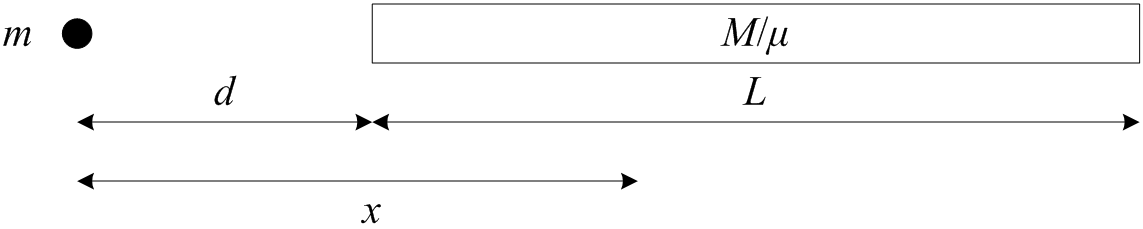
\includegraphics[height=1.5cm]{3.5.png}
\end{figure}
\end{example}

解:

小球可以视为质点,但细长杆不行,根据引力方程,假设细长杆的一个微元对小球的引力可以视为质点,则引力微元$dF=G\frac{m\cdot \mu dx}{x^2}$,整体引力:
\begin{align*}
F&=\int_d^{d+L}{G\frac{m\cdot \mu dx}{x^2}}=Gm\mu \int_d^{d+L}{\frac{1}{x^2}\cdot dx} \\
&=Gm\mu \left( \left. -\frac{1}{x} \right|_{d}^{d+L} \right) =Gm\mu \left( \frac{1}{d}-\frac{1}{d+L} \right)
\end{align*}

%============================================================
\subsection{第二宇宙速度}

\begin{example}
求第二宇宙速度,即脱离地球引力范围的最小速度。
\end{example}

解:

假设地球质量$M$,物体质量$m$,地球半径$R$,脱离地球引力范围即相当于飞至无限远。
结合能量守恒定律,物体飞至无限远引力做功即物体的初动能:
\[
\frac{1}{2}{mv_0}^2=\int_R^{+\infty}{F\left( r \right) dr}=\int_R^{+\infty}{G\frac{Mm}{r^2}dr}
\]
该问题从数学上看是一个无穷区间上的反常积分:
\begin{align*}
&\because \int_R^{+\infty}{G\frac{Mm}{r^2}dr}=GMm\left( \left. -\frac{1}{r} \right|_{R}^{+\infty} \right) =\frac{GMm}{R} \\
&\therefore v_0=\sqrt{\frac{2GM}{R}}=\sqrt{2gR}\approx 11.2\mathrm{km}/\mathrm{s}
\end{align*}
物体的初速度11.2km/s,即为第二宇宙速度。

%============================================================
\subsection{函数的平均值和均方根值}

之前我们讨论了离散量的算术平均值:
\[
\bar{x}=\frac{x_1+x_2+\cdots +x_n}{n}
\]
如果是连续量,如电流、功率,就涉及连续函数的平均值。

\begin{definition}[函数的平均值]
设函数$f\left( x \right) $在$\left[ a,b \right] $上连续,将$\left[ a,b \right] $等分为$n$个小区间$a=x_0<x_1<x_2<...<x_{n-1}<x_n=b$,记每个小区间的长度$\Delta x_i=\frac{b-a}{n}$,我们可以用:
\[
\frac{f\left( x_1 \right) +f\left( x_2 \right) +\cdots +f\left( x_n \right)}{n}=\frac{1}{n}\sum_{i=1}^n{f\left( x_i \right)}
\]
近似描述平均值,如果当$n\rightarrow \infty $时该和式有极限,我们就称该极限为{\bf 函数$f\left( x \right) $在$\left[ a,b \right] $上的平均值},记作$\bar{y}$,即:
\begin{align*}
\bar{y}:&=\underset{n\rightarrow \infty}{\lim}\frac{1}{n}\sum_{i=1}^n{f\left( x_i \right)}=\underset{n\rightarrow \infty}{\lim}\sum_{i=1}^n{\frac{f\left( x_i \right)}{n}} \\
&=\underset{n\rightarrow \infty}{\lim}\sum_{i=1}^n{\left[ f\left( x_i \right) \cdot \frac{\Delta x_i}{b-a} \right]}=\frac{1}{b-a}\underset{n\rightarrow \infty}{\lim}\sum_{i=1}^n{\left[ f\left( x_i \right) \cdot \Delta x_i \right]} \\
&=\frac{1}{b-a}\int_a^b{f\left( x \right) dx}
\end{align*}
\end{definition}

\begin{definition}[函数的均方根值]

若函数$f\left( x \right) $在$\left[ a,b \right] $上连续,我们称如下积分为{\bf 函数$f\left( x \right) $在$\left[ a,b \right] $上的均方根值},常记作RMS(Root Mean Square),即:
\[
RMS:=\sqrt{\frac{1}{b-a}\int_a^b{f^2\left( x \right) dx}}
\]
\end{definition}

物理上,我们通常用平均值表示一个物理量一段时间内的平均值,特别是周期物理量,用均方根值表示物理量的有效值。

~

\begin{example}
若交流电的电流$I\left( t \right) =I_m\sin \omega t$,$I_m$为峰值,计算在电阻$R$上的平均功率和有效电流。
\end{example}

解:

交流电的平均功率可以计算在一个周期$T=2\pi /\omega $内的功率的平均值,如下:
\begin{align*}
&\because P\left( t \right) =I^2\left( t \right) R=\left( I_m\sin \omega t \right) ^2R \\
&\therefore \bar{P}=\frac{1}{T}\int_0^T{P\left( t \right) dt}=\frac{\omega}{2\pi}\int_0^{2\pi /\omega}{\left( I_m\sin \omega t \right) ^2R\cdot dt}=\frac{1}{2}{I_m}^2R
\end{align*}
有效电流采用均方根值计算方式:
\[
\sqrt{\frac{1}{T}\int_0^T{I^2\left( t \right) \cdot dt}}=\sqrt{\frac{\omega}{2\pi}\int_0^{2\pi /\omega}{\left( I_m\sin \omega t \right) ^2\cdot dt}}=\frac{1}{\sqrt{2}}I_m
\]






\newpage
\section{本章小结}

本章介绍了积分。
其中,定积分是明确具备工程或物理意义的数学概念,能用于解决实际问题的数学工具。
但依照定积分的定义进行计算时,计算量非常大。
所以我们通过牛顿莱布尼兹公式引出不定积分的概念,给出了计算定积分的一个系统的方法,极大方便了计算。

\begin{itemize}
    \item 定积分:着重在理解其定义的几何、工程、物理等意义。
    \item 不定积分:学习和掌握各种求解不定积分的方法,不需要熟练,不定积分的计算是为后续微分方程准备的,其公式推导有现成软件。
\end{itemize}






\newpage
\section{习题}

\begin{exercise}
计算下列导数和极限:
\begin{enumerate}
    \item $\frac{d}{dx}\int_0^{x^2}{\sqrt{1+t^2}dt}$
    \item $\frac{d}{dx}\int_{\sin x}^{\cos x}{\cos \left( \pi t^2 \right) dt}$
    \item $\underset{x\rightarrow 0}{\lim}\frac{\int_0^x{\cos t^2dt}}{x}$
    \item $\underset{x\rightarrow +\infty}{\lim}\frac{\left( \int_0^x{e^{t^2}dt} \right) ^2}{\int_0^x{e^{2t^2}dt}}$
\end{enumerate}
\end{exercise}

解:

1.
\[
\frac{d}{dx}\int_0^{x^2}{\sqrt{1+t^2}dt}=\sqrt{1+\left( x^2 \right) ^2}\cdot \left( x^2 \right) '=2x\sqrt{1+x^4}
\]

2.
\begin{align*}
&\frac{d}{dx}\int_{\sin x}^{\cos x}{\cos \left( \pi t^2 \right) dt} \\
&=\frac{d}{dx}\int_{\sin x}^0{\cos \left( \pi t^2 \right) dt}+\frac{d}{dx}\int_0^{\cos x}{\cos \left( \pi t^2 \right) dt} \\
&=-\cos \left( \pi \sin ^2x \right) \cdot \cos x-\cos \left( \pi \cos ^2x \right) \cdot \sin x
\end{align*}

3.
\[
\underset{x\rightarrow 0}{\lim}\frac{\int_0^x{\cos t^2dt}}{x}=\underset{x\rightarrow 0}{\lim}\frac{\cos x^2\cdot 1}{1}=1
\]

4.
\begin{align*}
\underset{x\rightarrow +\infty}{\lim}\frac{\left( \int_0^x{e^{t^2}dt} \right) ^2}{\int_0^x{e^{2t^2}dt}}&=\underset{x\rightarrow +\infty}{\lim}\frac{2\left( \int_0^x{e^{t^2}dt} \right) \cdot e^{x^2}}{e^{2x^2}} \\
&=2\underset{x\rightarrow +\infty}{\lim}\frac{\int_0^x{e^{t^2}dt}}{e^{x^2}}=2\underset{x\rightarrow +\infty}{\lim}\frac{e^{x^2}\cdot 1}{2xe^{x^2}}=0
\end{align*}

\begin{tcolorbox}
主要是理解含积分复合函数的求导。
\end{tcolorbox}

~

\begin{exercise}
若方程$\int_0^y{e^tdt}+\int_0^x{\cos tdt}=0$确定函数$y=f\left( x \right) $,求$\frac{dy}{dx}$。
\end{exercise}

解:

大体思路是隐函数和积分复合函数的混合体,令隐函数$F\left( x,y \right) =\int_0^y{e^tdt}+\int_0^x{\cos tdt}=0$,则:
\begin{align*}
&\because \begin{cases}
	F_x=\frac{d}{dx}\left( \int_0^y{e^tdt}+\int_0^x{\cos tdt} \right) =e^y\cdot 0+\cos x\cdot 1=\cos x\\
	F_y=\frac{d}{dy}\left( \int_0^y{e^tdt}+\int_0^x{\cos tdt} \right) =e^y\cdot 1+\cos x\cdot 0=e^y\\
\end{cases} \\
&\therefore \frac{dy}{dx}=-\frac{F_x}{F_y}=-\frac{\cos y}{e^y}
\end{align*}

~

\begin{exercise}
若有一物体做直线运动,设其运动规律是$s=ct^3$,媒质阻力与速度的平方成正比,求物体由$s=0$运动至$s=b$时,克服阻力作的功。
\end{exercise}

解:

做功微元是$dW=F\cdot ds$,对路程积分,阻力$F$对路程$s$的表达式:
\[
F\left( s \right) =kv^2=k\left( \frac{ds}{dt} \right) ^2=k\left( 3ct^2 \right) ^2=9kc^2\left( \frac{s}{c} \right) ^{\frac{4}{3}}
\]
所以得到克服阻力作的功:
\[
W=\int_0^b{dW}=\int_0^b{9kc^2\left( \frac{s}{c} \right) ^{\frac{4}{3}}\cdot ds}=\frac{27}{7}kc^{\frac{2}{3}}b^{\frac{7}{3}}
\]










\chapter{常微分方程}

自然界中多数物理量在变化过程中其变化率和现存量有着关系,即$A\left( y \right) =B\left( y' \right) $。
所以,通过求解这个关系式就可以得出该物理量的函数。

本章要点:
\begin{itemize}
    \item 充分理解微分方程的定义和物理意义。
    \item 理解微分方程的求解思路。
    \item 学会推导一阶线性常微分方程的求解过程。
    \item 掌握一阶线性方程的求解公式和物理意义。
    \item 学会推导二阶常系数齐次线性方程的求解过程。
    \item 掌握二阶常系数齐次线性方程的求解公式和物理意义。
\end{itemize}

~

\newpage
\section{常微分方程}

函数描述量和量之间的关系,但在很多实际问题中这个函数关系无法直接找出,而是根据条件建立起量及其变化率之间的关系式,这就是微分方程。
通过求解微分方程得到函数关系。

本节要点:
\begin{itemize}
    \item 理解常微分方程的概念;
    \item 理解常微分方程的物理意义;
    \item 掌握一阶微分方程的求解思路和方法。
\end{itemize}

%============================================================
\subsection{常微分方程的概念}

\begin{definition}[微分方程]
我们将含有未知函数及其导数(或微分)的方程称为{\bf 微分方程}。
未知函数是一元函数的微分方程称为{\bf 常微分方程}。
未知函数的最高阶导数的阶数称为微分方程的{\bf 阶}。
如果微分方程是未知函数及其各阶导数的一次有理整式,则称之为{\bf n阶线性常微分方程}(简称{\bf n阶线性方程}),记作:
\[
F\left( x,y,y',y'',...,y^{\left( n \right)} \right) =0
\]
如果函数$y=f\left( x \right) $代入微分方程后等式成立,则称$y=f\left( x \right) $为该微分方程的{\bf 解}。
如果函数含有常数,且常数的个数和微分方程的阶数相同,这样的函数称为{\bf 通解},否则称为{\bf 特解}。
\end{definition}

“阶”和“线性”都是对未知函数及其导数而言,不是对自变量的要求。
“线性”只是未知函数及其各阶导数的一次有理,如$\sin y$、$\left( y' \right) ^2$、$yy'$、$e^{y''}$都不是线性。

%============================================================
\subsection{求解思路}

求解一阶微分方程的大体思路是将方程变成分离形式,即:
\[
f\left( y \right) dy=g\left( x \right) dx
\]
然后两边分别积分:
\[
\int{f\left( y \right) dy}=\int{g\left( x \right) dx}
\]
再分别求不定积分,最后得到:
\[
F\left( y \right) =G\left( x \right) +C
\]

%============================================================
\subsection{微分方程的物理意义}

通常一个物理量和其变化率有关,所以可以用一个微分方程描述,那么微分方程的通解就是这个物理量的数学表达式。

可以毫不夸张地说,宇宙里所有系统都可以用微分方程描述,这是有一个深层次原因的。
对于一个输入输出系统,输入的量并不是直接作用产生输出,往往会在系统中振荡几下再输出。
在系统论的角度,当刻的输出是当刻及之前的输入和之前的输出一起作用的结果,这种作用体现在数学模型上就是微分方程。

\begin{tcolorbox}
微分方程可以和《信号与系统》课程相互学习。
\end{tcolorbox}






\newpage
\section{一阶线性常微分方程}

全称“一阶线性常微分方程”:
\begin{itemize}
    \item 一阶:未知函数的最高阶导数为一阶导数;
    \item 线性:微分方程是未知函数及其导数的一次有理整式;
    \item 常:未知函数是一元函数。
\end{itemize}
由于本章所述均为一元函数,所以省去“常微分”,简称“一阶线性方程”。

一阶线性方程解法的总体思路是分离变量,通过把$dx$和$dy$分离到方程的两边,再求解积分化掉微分项$dx$和$dy$。
一阶线性方程的通解可以描述为:
\[
\text{一阶线性方程的通解} = \text{齐次方程的通解} + \text{非齐次方程的一个特解}
\]
为了得到这个方法,本节先从分离变量开始,讲到齐次方程,最后推导出一阶线性方程的求解公式。

本节要点:
\begin{itemize}
    \item 熟悉一阶线性方程的形式;
    \item 推导一阶线性方程的通解;
    \item 体会一阶线性方程的物理意义。
\end{itemize}

%============================================================
\subsection{一阶齐次线性方程}

\begin{definition}[一阶齐次线性方程]
形如
\[
\frac{dy}{dx}+P\left( x \right) y=0
\]
的微分方程称为{\bf 一阶齐次线性方程},其中$y=f\left( x \right) $。
\end{definition}

\begin{tcolorbox}
“齐次”指的是没有和$y$无关的项。
\end{tcolorbox}

求解过程如下:
\begin{enumerate}
    \item 分离变量:
    \[
    \frac{1}{y}dy=-P\left( x \right) dx
    \]
    \item 两边分别求不定积分:
    \[
    \ln \left| y \right|=-\int{P\left( x \right) dx}+C
    \]
    \item 两边取$e$的指数,得到通解:
    \[
    y=Ce^{-\int{P\left( x \right) dx}}
    \]
\end{enumerate}

特别地,当$P\left( x \right) \equiv P\ne 0$时,方程中无自变量$x$,方程变成:
\[
\frac{dy}{dx}+Py=0
\]
它是一阶齐次线性方程的特殊形式——{\bf 一阶常系数齐次线性方程},即$y$的系数不是一个关于$x$的函数,而是一个固定值,用通解公式易得通解:
\[
y=Ce^{-Px}
\]
是一个很典型的指数函数,讨论$x\in \left( 0,+\infty \right) $的时候:
\begin{itemize}
    \item 当$P>0$,$y$单调递减并从$C$趋向0,相当于引入一个负反馈;
    \item 当$P<0$,$y$单调递增并从$C$趋向$+\infty $,相当于引入一个正反馈;
    \item 当$P=0$,方程变成$\frac{dy}{dx}=0$,解为$y=C$。
\end{itemize}

\begin{tcolorbox}
在物理角度看方程$\frac{dy}{dx}+Py=0$的解,如果一个系统没有输入,仅靠存量作用产生输出(《信号与系统》理论中称为零输入响应),往往会以指数形式衰减,比如放射性物质衰变公式。
\end{tcolorbox}

%============================================================
\subsection{一阶非齐次线性方程}

\begin{definition}[一阶非齐次线性方程]
形如
\[
\frac{dy}{dx}+P\left( x \right) y=Q\left( x \right)
\]
的微分方程称为{\bf 一阶非齐次线性方程},其中$y=f\left( x \right) $。
\end{definition}

\begin{tcolorbox}
“非齐次”指的是有了一个和$y$无关的项$Q\left( x \right) $。
\end{tcolorbox}

求解过程如下:
\begin{enumerate}
    \item 求得对应的齐次方程的通解:
    \[
    y=Ce^{-\int{P\left( x \right) dx}}
    \]
    \item 将常数$C$变为待定函数$C=\left( x \right) $,代入上式:
    \[
    y=C\left( x \right) e^{-\int{P\left( x \right) dx}}
    \]
    \item 将该函数代入微分方程求得:
    \[
    C\left( x \right) =\int{Q\left( x \right) e^{\int{P\left( x \right) dx}}dx}+C
    \]
    \item 得到通解:
    \[
    y=e^{-\int{P\left( x \right) dx}}\cdot \left[ \int{Q\left( x \right) e^{\int{P\left( x \right) dx}}dx}+C \right]
    \]
\end{enumerate}

特别地,当$P\left( x \right) \equiv P,Q\left( x \right) \equiv Q$时,方程中无自变量$x$,方程变成:
\[
\frac{dy}{dx}+Py=Q
\]
它是一阶非齐次线性方程的特殊形式——{\bf 一阶常系数非齐次线性方程},即$y$的系数和无关项是一个固定值,用通解公式易得通解:
\[
y=Ce^{-Px}+\frac{Q}{P}
\]
在典型的指数函数的基础上上抬了$Q/P$,讨论$x\in \left( 0,+\infty \right) $的时候:
\begin{itemize}
    \item 当$P>0$,$y$单调递减并从$C+Q/P$趋向$Q/P$,相当于引入一个负反馈;
    \item 当$P<0$,$y$单调递增并从$C+Q/P$趋向$+\infty $,相当于引入一个正反馈。
\end{itemize}
和一阶常系数齐次线性方程对比看,整个系统有一个“固定能量”。

一阶线性常微分方程由于只包含一阶导数,函数的变化率单一,所以不会像二阶一样发生振荡。

%============================================================
\subsection{一阶线性方程及通解形式}

一阶齐次线性方程:
\begin{align*}
&\text{方程:} \quad \frac{dy}{dx}+P\left( x \right) y=0 \\
&\text{通解:} \quad y=Ce^{-\int{P\left( x \right) dx}}
\end{align*}

一阶常系数齐次线性方程:
\begin{align*}
&\text{方程:} \quad \frac{dy}{dx}+Py=0 \\
&\text{通解:} \quad y=Ce^{-Px}
\end{align*}

一阶非齐次线性方程:
\begin{align*}
&\text{方程:} \quad \frac{dy}{dx}+P\left( x \right) y=Q\left( x \right) \\
&\text{通解:} \quad y=e^{-\int{P\left( x \right) dx}}\cdot \left[ \int{Q\left( x \right) e^{\int{P\left( x \right) dx}}dx}+C \right]
\end{align*}

一阶常系数非齐次线性方程:
\begin{align*}
&\text{方程:} \quad \frac{dy}{dx}+Py=Q \\
&\text{通解:} \quad y=Ce^{-Px}+\frac{Q}{P}
\end{align*}






\newpage
\section{二阶常系数齐次线性方程}

对于二阶线性方程,本节只讨论二阶常系数齐次线性方程。

本节要点:
\begin{itemize}
    \item 熟悉二阶线性方程的形式;
    \item 推导二阶线性方程的通解;
    \item 体会二阶线性方程的物理意义。
\end{itemize}

%============================================================
\subsection{二阶常系数齐次线性方程}

\begin{definition}[二阶常系数齐次线性方程]
形如
\[
\frac{d^2y}{dx^2}+P\frac{dy}{dx}+Qy=0
\]
的微分方程称为{\bf 二阶常系数齐次线性方程},其中$y=f\left( x \right) $。
\end{definition}

该微分方程的求解,全靠“凑”,求解过程如下:
\begin{enumerate}
    \item 假设函数形如:
    \[
    y=e^{rx}
    \]
    \item 将$y,y',y''$代入方程得到:
    \[
    r^2e^{rx}+Pre^{rx}+Qe^{rx}=0
    \]
    \item 由于$e^{rx}>0$,所以要使方程成立,即为求解特征方程:
    \[
    r^2+Pr+Q=0
    \]
    \item 得到两个根:
    \[
    r=\frac{-P\pm \sqrt{P^2-4Q}}{2}
    \]
\end{enumerate}

根据特征方程的根,当$Q\ne 0$时,通解分成以下4个情形:
\begin{itemize}
    \item $P^2>4Q$,$r$有两个不等实根$r_{1,2}=\frac{-P\pm \sqrt{P^2-4Q}}{2}$,于是
    \[
    y=C_1e^{r_1x}+C_2e^{r_2x}
    \]
    物理上对应大阻尼,物理量呈指数衰减趋于0,没有振荡。
    \item $P^2=4Q$,$r$有两个相等实根$r_{1,2}=-\frac{P}{2}$,于是
    \[
    y=\left( C_1+C_2 \right) e^{-Px/2}
    \]
    物理上对应临界阻尼,同上。
    \item $P^2<4Q$,$r$有两个共轭复根$r_{1,2}=\frac{-P\pm i\sqrt{4Q-P^2}}{2}$,于是
    \[
    y=e^{-\frac{P}{2}x}\cdot \left[ C_1\cos \frac{x\sqrt{4Q-P^2}}{2}+C_2\sin \frac{x\sqrt{4Q-P^2}}{2} \right]
    \]
    物理上对应小阻尼,物理量以指数衰减的方式振荡趋于0。
    \item $P=0$,$r$为纯虚根$r_{1,2}=\pm i\sqrt{Q}$,于是
    \[
    y=C_1\cos \left( x\sqrt{Q} \right) +C_2\sin \left( x\sqrt{Q} \right)
    \]
    物理上对应无阻尼振荡。
\end{itemize}

实部决定了{\it y}是否有衰减阻尼,虚部决定了{\it y}是否有振荡。
很多物理过程都可以用二阶常系数齐次线性方程描述,如弹簧震动、RLC电路等。

特别地,当$Q=0$时方程化为:
\[
\frac{d^2y}{dx^2}+P\frac{dy}{dx}=0
\]
求解特征方程$r^2+Pr=0$得到两个根$r=-P\mathrm{or}0$,于是解为:
\begin{align*}
&y=Ce^{-Px} \\
&y=C
\end{align*}

%============================================================
\subsection{PQ关系总结}

将$P,Q$及其关系总结如下:
\begin{itemize}
    \item 当$Q\ne 0,P\ne 0$时,方程为$\frac{d^2y}{dx^2}+P\frac{dy}{dx}+Qy=0$:
    \begin{itemize}
        \item 当$P^2>4Q$时,通解表现为衰减$y=C_1e^{r_1x}+C_2e^{r_2x}$;
        \item 当$P^2=4Q$时,通解表现为衰减$y=\left( C_1+C_2 \right) e^{-Px/2}$;
        \item 当$P^2<4Q$时,通解表现为振荡衰减
        \[
        y=e^{-\frac{P}{2}x}\cdot \left[ C_1\cos \frac{x\sqrt{4Q-P^2}}{2}+C_2\sin \frac{x\sqrt{4Q-P^2}}{2} \right]
        \]
    \end{itemize}
    \item 当$Q\ne 0,P=0$时,方程为$\frac{d^2y}{dx^2}+Qy=0$:
    \begin{itemize}
        \item 通解表现为振荡$y=C_1\cos \left( x\sqrt{Q} \right) +C_2\sin \left( x\sqrt{Q} \right) $。
    \end{itemize}
    \item 当$Q=0,P\ne 0$时,方程为$\frac{d^2y}{dx^2}+P\frac{dy}{dx}=0$:
    \begin{itemize}
        \item 通解表现为衰减$y=Ce^{-Px}$。
    \end{itemize}
    \item 当$Q=0,P=0$时,方程为$\frac{d^2y}{dx^2}=0$:
    \begin{itemize}
        \item 通解表现为恒定$y=C$。
    \end{itemize}
\end{itemize}

~

不难发现:
\begin{itemize}
    \item $P$表示阻尼,如果$P\ne 0$则衰减,如果$P=0$则恒定;
    \item $Q$表示振荡,如果$Q\ne 0$则振荡,如果$Q=0$则无振荡;
    \item 特别地,当$P^2\geqslant 4Q$,阻尼大过振荡,也振荡不起来。
\end{itemize}






\newpage
\section{一阶二阶微分方程的物理意义}

我们讨论一阶常系数齐次线性方程和二阶常系数齐次线性方程:
\begin{align*}
&\frac{dy}{dx}+Py=0 \\
&\frac{d^2y}{dx^2}+P\frac{dy}{dx}+Qy=0
\end{align*}

总体来讲,当系统有能量耗散时,都可以用常系数齐次线性微分方程描述。
如果系统内部只有一种能量形式,这种耗散表示为一阶方程,结果以指数形式耗散,$P$表示耗散速度。
如果有两种能量形式,表现为二阶方程,以指数振荡形式耗散,振荡表现为两种能量形式之间的转换,$P$表示耗散速度,$Q$代表振荡。






\newpage
\section{本章小结}

本章介绍非常简单的微分方程。

微分方程在各个工程方面均有广泛用途,如电子电路、机械、药代动力、经济、人口。
如何将某个领域的具体问题转化为数学问题,是数学建模讲述的。

微积分本身不涉及数学建模。
本章的讲述在建模之后,即得到方程之后,对方程的求解,附带介绍了解的物理意义。

“教材\cite{book1}”中有很多例子,可以反复细看:
\begin{itemize}
    \item 放射性衰变(P311、P318);
    \item 正交轨线(P318);
    \item 伯努利方程(P328);
    \item 悬链线(P333);
    \item 振动问题(P354);
    \item 鱼雷击舰问题(P363);
    \item 人口增长模型和逻辑斯蒂Logistic方程(P365)。
\end{itemize}










\chapter{矢量与空间}

本章讨论三维空间和三维矢量的一些基础概念,这些概念是多元函数微积分的基础。

本章要点:
\begin{itemize}
    \item 矢量及其运算。
    \item 三维空间中的点、直线和平面。
    \item 数量场和矢量场。
\end{itemize}

~

\newpage
\section{直角坐标系}

本节介绍直角坐标系。

%============================================================
\subsection{直角坐标系的概念}

通常,三维空间的直角坐标系的方向用右手规定。
空间中的点可以用一个有序三元实数组表示,同时也可以用一个{\bf 3维列向量}(本笔记也称{\bf 矢量})表示,于是下面两个表示方法等价:
\begin{itemize}
    \item 点$\mathrm{P}\left( x,y,z \right) $,有时也可以简单写成$\mathrm{P}$;
    \item 矢量$\boldsymbol{p}=\left( x\,\,y\,\,z \right) ^T$。
\end{itemize}
其中,$x,y,z\in \mathbb{R} $表示点$\mathrm{P}$的{\it xyz}轴坐标。

我们采用欧几里得范数(也即内积引导的范数)定义两个点$\mathrm{P},\mathrm{Q}$的距离,记为$\left\| \mathrm{PQ} \right\| $,有:
\begin{align*}
\left\| \mathrm{PQ} \right\| :&=\left\| \boldsymbol{p}-\boldsymbol{q} \right\| \\
&=\sqrt{\left( \boldsymbol{p}-\boldsymbol{q} \right) ^T\left( \boldsymbol{p}-\boldsymbol{q} \right)}=\sqrt{\left( x_{\boldsymbol{p}}-x_{\boldsymbol{q}} \right) ^2+\left( y_{\boldsymbol{p}}-y_{\boldsymbol{q}} \right) ^2+\left( z_{\boldsymbol{p}}-z_{\boldsymbol{q}} \right) ^2}
\end{align*}

\begin{tcolorbox}
直角坐标系的右手方向,只是规定!规定!规定!纯人为规定!
\end{tcolorbox}






\newpage
\section{矢量}

本节介绍矢量及其运算法则。
矢量是量化空间的基础,更是多元函数微积分的基础。

本节要点:
\begin{itemize}
    \item 掌握矢量的定义;
    \item 掌握矢量的运算;
    \item 理解矢量内积和外积的几何意义;
    \item 理解矢量之间的关系——平行和垂直。
\end{itemize}

%============================================================
\subsection{矢量和方向余弦}

\begin{definition}[矢量]
我们称既有大小又有方向的量为{\bf 矢量},三维空间中我们采用列向量的表示方式:
\[
\boldsymbol{a}:=\left( \begin{array}{c}
	x\\
	y\\
	z\\
\end{array} \right)
\]
为排版方便,也可记为行向量的转置:
\[
\boldsymbol{a}:=\left( x\,\,y\,\,z \right) ^T
\]
\end{definition}

矢量是空间几何的代数化基础。
空间的点可以通过矢量描述,空间的面和线可以通过矢量方程描述,它们之间的关系可以通过矢量运算判断。

\begin{definition}
我们采用标量积的形式定义{\bf 矢量的模},记作$\left\| \boldsymbol{a} \right\| $,即:
\[
\left\| \boldsymbol{a} \right\| :=\sqrt{\boldsymbol{a}^T\boldsymbol{a}}=\sqrt{x^2+y^2+z^2}
\]
也称{\bf 长度}。特别地,当$\left\| \boldsymbol{a} \right\| =1$时称为{\bf 单位矢量}。

称矢量:
\[
\left( \begin{array}{c}
	\cos \alpha\\
	\cos \beta\\
	\cos \gamma\\
\end{array} \right) =\left( \begin{array}{c}
	\frac{x}{\left\| \boldsymbol{a} \right\|}\\
	\frac{y}{\left\| \boldsymbol{a} \right\|}\\
	\frac{z}{\left\| \boldsymbol{a} \right\|}\\
\end{array} \right) \qquad \alpha ,\beta ,\gamma \in \left[ 0,\pi \right]
\]
为{\bf 矢量$\boldsymbol{a}$的方向余弦},方向余弦中的三个角是矢量$\boldsymbol{a}$分别和{\it xyz}三个轴所成的角度,方向余弦本身为单位矢量。
\end{definition}

我们规定:
\begin{itemize}
    \item 零矢量:$\mathbf{0}=\left( 0\,\,0\,\,0 \right) ^T$
    \item 单位矢量:$\mathbf{a}=\frac{\boldsymbol{a}}{\left\| \boldsymbol{a} \right\|}$
    \item 数乘:$\lambda \boldsymbol{a}=\lambda \left( x\,\,y\,\,z \right) ^T=\left( \lambda x\,\,\lambda y\,\,\lambda z \right) ^T$
    \item 基矢量:$\mathbf{i}=\left( 1\,\,0\,\,0 \right) ^T \quad \mathbf{j}=\left( 0\,\,1\,\,0 \right) ^T \quad \mathbf{k}=\left( 0\,\,0\,\,1 \right) ^T$
\end{itemize}
于是任何矢量均可以用基矢量写成:
\[
\boldsymbol{a}=x\mathbf{i}+y\mathbf{j}+z\mathbf{k}
\]

\begin{tcolorbox}
注意,我们使用粗体表示单位矢量,而不是一般教材用的下标0。
因为我们将$\boldsymbol{p},\boldsymbol{p}_0$用于之后概念的定义,如$x,x_0$用于一元函数微积分中一样。
\end{tcolorbox}

%============================================================
\subsection{矢量的加法}

\begin{definition}[加法]
我们将矢量的{\bf 加法}定义为矢量中所有对应元素相加,记作$\boldsymbol{a}+\boldsymbol{b}$,即:
\begin{align*}
\boldsymbol{a}+\boldsymbol{b}:&=\left( x_{\boldsymbol{a}}\,\,y_{\boldsymbol{a}}\,\,z_{\boldsymbol{a}} \right) ^T+\left( x_{\boldsymbol{b}}\,\,y_{\boldsymbol{b}}\,\,z_{\boldsymbol{b}} \right) ^T \\
&=\left( x_{\boldsymbol{a}}+x_{\boldsymbol{b}} \quad y_{\boldsymbol{a}}+y_{\boldsymbol{b}} \quad z_{\boldsymbol{a}}+z_{\boldsymbol{b}} \right) ^T
\end{align*}
\end{definition}

注意:
\begin{itemize}
    \item 矢量相加仍为矢量;
    \item 几何上的结果是两个矢量构成的平行四边形的对角线。
\end{itemize}

运算法则:
\begin{align*}
&\boldsymbol{a}+\boldsymbol{b}=\boldsymbol{b}+\boldsymbol{a} \\
&\boldsymbol{a}+\left( \boldsymbol{b}+\boldsymbol{c} \right) =\left( \boldsymbol{a}+\boldsymbol{b} \right) +\boldsymbol{c} \\
&\lambda \left( \boldsymbol{a}+\boldsymbol{b} \right) =\lambda \boldsymbol{a}+\lambda \boldsymbol{b} \\
&\lambda \left( \mu \boldsymbol{a} \right) =\left( \lambda \mu \right) \boldsymbol{a} \\
&\left\| \boldsymbol{a}+\boldsymbol{b} \right\| \leqslant \left\| \boldsymbol{a} \right\| +\left\| \boldsymbol{b} \right\|
\end{align*}

%============================================================
\subsection{矢量的内积}

\begin{definition}[内积]
我们采用标量积定义矢量的{\bf 内积},记作$\boldsymbol{a}^T\boldsymbol{b}$,即:
\[
\boldsymbol{a}^T\boldsymbol{b}:=\left( x_{\boldsymbol{a}}\,\,y_{\boldsymbol{a}}\,\,z_{\boldsymbol{a}} \right) \left( x_{\boldsymbol{b}}\,\,y_{\boldsymbol{b}}\,\,z_{\boldsymbol{b}} \right) ^T=x_{\boldsymbol{a}}x_{\boldsymbol{b}}+y_{\boldsymbol{a}}y_{\boldsymbol{b}}+z_{\boldsymbol{a}}z_{\boldsymbol{b}}
\]
也称{\bf 数量积},也可记为$\boldsymbol{a}\cdot \boldsymbol{b}$,于是又称{\bf 点积}。
\end{definition}

\begin{tcolorbox}
有些教材使用$\boldsymbol{a}\cdot \boldsymbol{b}$表示内积,但我们用$\boldsymbol{a}^T\boldsymbol{b}$,好处是$\boldsymbol{a}^T\boldsymbol{b}\cdot dl$这样的被积式清晰无歧义。
\end{tcolorbox}

\begin{theorem}
矢量内积等于矢量的模的积再乘以它们夹角的余弦,即:
\[
\boldsymbol{a}^T\boldsymbol{b}=\left\| \boldsymbol{a} \right\| \left\| \boldsymbol{b} \right\| \cos \theta \qquad \theta \in \left[ 0,\pi \right]
\]
\end{theorem}

矢量内积常用于判断两个矢量的空间关系,相互垂直还是平行。

注意:
\begin{itemize}
    \item 矢量内积的结果为标量;
    \item 几何上,内积可以看成$\boldsymbol{a}$在$\boldsymbol{b}$的方向上的投影值$\left\| \boldsymbol{a} \right\| \cos \theta $和$\left\| \boldsymbol{b} \right\| $的乘积;
    \item 空间上,
    \begin{itemize}
        \item 两个矢量垂直$\Leftrightarrow \theta =\pi /2\Leftrightarrow \boldsymbol{a}^T\boldsymbol{b}=0$,记为$\boldsymbol{a}\bot \boldsymbol{b}$,称为两个矢量{\bf 正交},
        \item 两个矢量平行$\Leftrightarrow \theta =0\mathrm{or}\pi \Leftrightarrow \boldsymbol{a}=\lambda \boldsymbol{b}$,记为$\boldsymbol{a}\parallel \boldsymbol{b}$,称为两个矢量{\bf 平行}(或{\bf 共线})。
    \end{itemize}
    \item 根据内积公式可以得到,
    \begin{itemize}
        \item 若$\boldsymbol{a}^T\boldsymbol{b}>0$,则两个矢量方向基本相同,夹角0°~90°,
        \item 若$\boldsymbol{a}^T\boldsymbol{b}=0$,则两个矢量相互垂直,夹角为90°,
        \item 若$\boldsymbol{a}^T\boldsymbol{b}<0$,则两个矢量方向基本相反,夹角90°~180°。
    \end{itemize}
\end{itemize}

对于单位矢量特别有:
\begin{align*}
&\mathbf{i}^T\mathbf{i}=\mathbf{j}^T\mathbf{j}=\mathbf{k}^T\mathbf{k}=1 \\
&\mathbf{i}^T\mathbf{j}=\mathbf{j}^T\mathbf{k}=\mathbf{k}^T\mathbf{i}=0
\end{align*}

运算法则:
\begin{align*}
&\boldsymbol{a}^T\boldsymbol{b}=\boldsymbol{b}^T\boldsymbol{a} \\
&\boldsymbol{a}^T\left( \boldsymbol{b}+\boldsymbol{c} \right) =\boldsymbol{a}^T\boldsymbol{b}+\boldsymbol{a}^T\boldsymbol{c} \\
&\left( \lambda \boldsymbol{a} \right) ^T\left( \mu \boldsymbol{b} \right) =\left( \lambda \mu \right) \boldsymbol{a}^T\boldsymbol{b} \\
&\boldsymbol{a}^T\boldsymbol{a}=\left\| \boldsymbol{a} \right\| ^2
\end{align*}

\begin{tcolorbox}
矢量内积这个概念源于考察矢量场对边界的扩张或收缩的效果。
\end{tcolorbox}

%============================================================
\subsection{矢量的外积}

\begin{definition}[外积]
我们采用行列式定义{\bf 外积},记作$\boldsymbol{a}\times \boldsymbol{b}$,即:
\begin{align*}
\boldsymbol{a}\times \boldsymbol{b}:&=\left( x_{\boldsymbol{a}}\,\,y_{\boldsymbol{a}}\,\,z_{\boldsymbol{a}} \right) \times \left( x_{\boldsymbol{b}}\,\,y_{\boldsymbol{b}}\,\,z_{\boldsymbol{b}} \right) ^T\\
&=\left| \begin{matrix}
	\mathbf{i}&		\mathbf{j}&		\mathbf{k}\\
	x_{\boldsymbol{a}}&		y_{\boldsymbol{a}}&		z_{\boldsymbol{a}}\\
	x_{\boldsymbol{b}}&		y_{\boldsymbol{b}}&		z_{\boldsymbol{b}}\\
\end{matrix} \right|=\left( \begin{array}{c}
	y_{\boldsymbol{a}}z_{\boldsymbol{b}}-z_{\boldsymbol{a}}y_{\boldsymbol{b}}\\
	z_{\boldsymbol{a}}x_{\boldsymbol{b}}-x_{\boldsymbol{a}}z_{\boldsymbol{b}}\\
	x_{\boldsymbol{a}}y_{\boldsymbol{b}}-y_{\boldsymbol{a}}x_{\boldsymbol{b}}\\
\end{array} \right)
\end{align*}
又称{\bf 叉积}、{\bf 矢量积}、{\bf 向量积}。
\end{definition}

\begin{theorem}
矢量外积的模等于矢量的模的积再乘以它们夹角的正弦,即:
\[
\left\| \boldsymbol{a}\times \boldsymbol{b} \right\| =\left\| \boldsymbol{a} \right\| \left\| \boldsymbol{b} \right\| \sin \theta \qquad \theta \in \left[ 0,\pi \right]
\]
\end{theorem}

注意:
\begin{itemize}
    \item 矢量外积的结果还是为矢量;
    \item 外积的方向垂直于$\boldsymbol{a},\boldsymbol{b}$构成的平面,符合“右手法则”,右手握拳由$\boldsymbol{a}$转向$\boldsymbol{b}$,拇指方向为外积方向,故也称为{\bf 法向量};
    \item 外积的大小为$\boldsymbol{a},\boldsymbol{b}$构成的平行四边形面积,当$\left\| \boldsymbol{a}\times \boldsymbol{b} \right\| =0$时,表示$\boldsymbol{a},\boldsymbol{b}$平行;
    \item 矢量外积常用于构建一个平面的法向矢量,当然也可以判断两个矢量是否平行,但不常用。
\end{itemize}

\begin{tcolorbox}
矢量外积的方向的“右手法则”是直角坐标系的“右手法则”的必然结果。
\end{tcolorbox}

对于单位矢量特别有:
\begin{align*}
&\mathbf{i}\times \mathbf{i}=\mathbf{j}\times \mathbf{j}=\mathbf{k}\times \mathbf{k}=0 \\
&\mathbf{i}\times \mathbf{j}=\mathbf{k} \\
&\mathbf{j}\times \mathbf{k}=\mathbf{i} \\
&\mathbf{k}\times \mathbf{i}=\mathbf{j}
\end{align*}

运算法则:
\begin{align*}
&\boldsymbol{a}\times \boldsymbol{b}=-\boldsymbol{b}\times \boldsymbol{a} \\
&\boldsymbol{a}\times \left( \boldsymbol{b}+\boldsymbol{c} \right) =\boldsymbol{a}\times \boldsymbol{b}+\boldsymbol{a}\times \boldsymbol{c} \\
&\boldsymbol{a}\times \boldsymbol{a}=\mathbf{0}
\end{align*}

\begin{tcolorbox}
矢量外积这个概念源于考察矢量场对区域自旋的效果。
\end{tcolorbox}

%============================================================
\subsection{内积和外积的比较}

考察内积和外积,内积和外积的大小的平方和是以$\boldsymbol{a},\boldsymbol{b}$长度构成的长方形的面积的平方。
\begin{align*}
&\because \begin{cases}
	\boldsymbol{a}^T\boldsymbol{b}=\left\| \boldsymbol{a} \right\| \left\| \boldsymbol{b} \right\| \cos \theta\\
	\left\| \boldsymbol{a}\times \boldsymbol{b} \right\| =\left\| \boldsymbol{a} \right\| \left\| \boldsymbol{b} \right\| \sin \theta\\
\end{cases} \\
&\therefore \left( \boldsymbol{a}^T\boldsymbol{b} \right) ^2+\left\| \boldsymbol{a}\times \boldsymbol{b} \right\| ^2=\left\| \boldsymbol{a} \right\| ^2\left\| \boldsymbol{b} \right\| ^2
\end{align*}
该关系式说明,内积和外积是一对关系,是一个本源分裂出来的两个概念。
物理意义上,是矢量场对区域的两个作用(收扩作用和自旋作用)的反映。
矢量场对一个区域的膨胀或收缩的效应,会用到内积运算,对该区域的自旋效应,会用到外积运算。






\newpage
\section{点、直线和平面}

本节介绍两个三维空间中最基础的几何体——点、直线和平面。

本节要点:
\begin{itemize}
    \item 掌握点、直线和平面的矢量表达式。
\end{itemize}

%============================================================
\subsection{点}

\begin{definition}[点]
三维空间的点用三个坐标值描述,通常写为$\mathrm{P}\left( x,y,z \right) $,也可缩写为“点$\mathrm{P}$”,也可以用矢量表示为“点$\boldsymbol{p}=\left( x\,\,y\,\,z \right) ^T$”。
\end{definition}

为符合矢量的加法运算法则,规定过两点$\mathrm{P}_1\left( x_1,y_1,z_1 \right) ,\mathrm{P}_2\left( x_2,y_2,z_2 \right) $且方向从$\mathrm{P}_1$到$\mathrm{P}_2$的直线,写成:
\begin{align*}
\overrightarrow{\mathrm{P}_1\mathrm{P}_2}:&=\boldsymbol{p}_2-\boldsymbol{p}_1 \\
&=\left( x_2\,\,y_2\,\,z_2 \right) ^T-\left( x_1\,\,y_1\,\,z_1 \right) ^T \\
&=\left( x_2-x_1 \quad y_2-y_1 \quad z_2-z_1 \right) ^T
\end{align*}
如果方向从$\mathrm{P}_2$到$\mathrm{P}_1$,则有$\overrightarrow{\mathrm{P}_2\mathrm{P}_1}=\boldsymbol{p}_1-\boldsymbol{p}_2=-\overrightarrow{\mathrm{P}_1\mathrm{P}_2}$。

\begin{figure}[h]
\centering
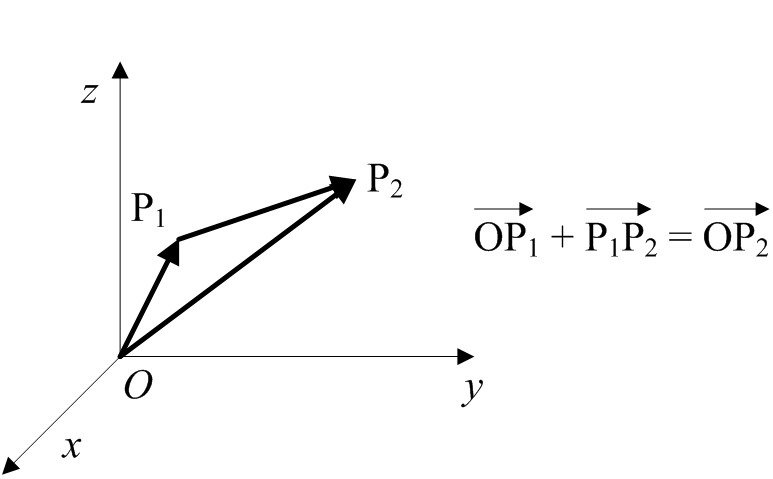
\includegraphics[height=4cm]{5.1.png}
\end{figure}

%============================================================
\subsection{直线方程}

\begin{definition}[直线方程]
若空间中两点$\boldsymbol{p},\boldsymbol{p}_0$构成的直线$\boldsymbol{p}-\boldsymbol{p}_0$和方向$\boldsymbol{n}=\left( A\,\,B\,\,C \right) ^T$平行,这些点构成的几何体称为{\bf 直线},用矢量方程描述为:
\[
\boldsymbol{p}-\boldsymbol{p}_0=\lambda \boldsymbol{n}
\]
展开后:
\[
\left( \begin{array}{c}
	x\\
	y\\
	z\\
\end{array} \right) -\left( \begin{array}{c}
	x_0\\
	y_0\\
	z_0\\
\end{array} \right) =\lambda \left( \begin{array}{c}
	A\\
	B\\
	C\\
\end{array} \right) \quad \text{或} \quad \frac{x-x_0}{A}=\frac{y-y_0}{B}=\frac{z-z_0}{C}
\]
称为{\bf 直线方程},其中:
\begin{itemize}
    \item $\boldsymbol{n}=\left( A\,\,B\,\,C \right) ^T$:直线的方向;
    \item $\boldsymbol{p}_0=\left( x_0\,\,y_0\,\,z_0 \right) ^T$:已知的直线上的点。
\end{itemize}
\end{definition}

若两直线平行,则两个矢量方向可以一致也可以相反。
如无特别情况,我们取一致的方向。

直线的另一种表达方式是两个平面的交线,若有两个平面:
\[
\begin{cases}
	A_1x+B_1y+C_1z+D_1=0\\
	A_2x+B_2y+C_2z+D_2=0\\
\end{cases}
\]
转化成点向式方程的步骤:
\begin{enumerate}
    \item 找出直线上的点$\boldsymbol{p}_0=\left( x_0\,\,y_0\,\,z_0 \right) ^T$,通常方便起见取$z_0=0$计算。
    \item 找出方向,直线的方向$\boldsymbol{n}=\left( A\,\,B\,\,C \right) ^T$和两个平面的法向构成的平面垂直,即:
    \[
    \boldsymbol{n}=\boldsymbol{n}_1\times \boldsymbol{n}_2=\left| \begin{matrix}
        \mathbf{i}&		\mathbf{j}&		\mathbf{k}\\
        A_1&		B_1&		C_1\\
        A_2&		B_2&		C_2\\
    \end{matrix} \right|
    \]
\end{enumerate}

%============================================================
\subsection{平面方程}

\begin{definition}[平面方程]
若点$\boldsymbol{p},\boldsymbol{p}_0$构成的直线$\boldsymbol{p}-\boldsymbol{p}_0$和方向$\boldsymbol{n}=\left( A\,\,B\,\,C \right) ^T$(称为{\bf 该平面的法向方向})垂直,这些点构成的几何体称为{\bf 平面},用矢量方程描述为:
\[
\left( \boldsymbol{p}-\boldsymbol{p}_0 \right) ^T\boldsymbol{n}=0
\]
展开后:
\begin{align*}
A\left( x-x_0 \right) +B\left( y-y_0 \right) +C\left( z-z_0 \right) =0 \quad \text{或} \quad Ax+By+Cz+D=0
\end{align*}
称为{\bf 平面方程},其中:
\begin{itemize}
    \item $\boldsymbol{p}-\boldsymbol{p}_0$:平面的法向;
    \item $\boldsymbol{p}_0=\left( x_0\,\,y_0\,\,z_0 \right) ^T$:已知的平面上的点。
\end{itemize}
\end{definition}

特别地,当平面和{\it xyz}三轴分别交于$x_0,y_0,z_0$,则可以写成截距式:
\[
\frac{x}{x_0}+\frac{y}{y_0}+\frac{z}{z_0}=1
\]

%============================================================
\subsection{曲线方程和曲面方程}

\begin{definition}[曲面方程]
三维空间中的曲面都可以描述为关于点$\boldsymbol{p}$的隐函数,如:
\[
F\left( \boldsymbol{p} \right) =0 \quad \text{或} \quad F\left( x,y,z \right) =0 \quad \text{或} \quad z=z\left( x,y \right)
\]
称为{\bf 曲面方程}。
\end{definition}

\begin{definition}[曲线方程]
在曲面方程中,$z$和$x,y$有约束关系,$x,y$之间并没有约束关系。
如果$x,y$之间还有约束关系,则曲面退化为曲线,上述表达式变为:
\[
F\left( x,y\left( x \right) ,z\left(y\left( x \right) \right) \right) =0 \quad \text{或} \quad z=z\left( x,y\left( x \right) \right)
\]
称为{\bf 曲线方程},更一般地,我们写成:
\[
\left\{ \begin{array}{c}
	x=x\left( t \right)\\
	y=y\left( t \right)\\
	z=z\left( t \right)\\
\end{array} \right.
\]
\end{definition}

\begin{tcolorbox}
这里并不刻意区分直线和平面的方向,直线的前后方向、平面的两侧方向,现在来讲都没有意义。
到了环流量和通量(即第二类曲线曲面积分),再规定线和面的方向。
\end{tcolorbox}






\newpage
\section{数量场和矢量场}

以三维空间为例:
\begin{itemize}
    \item 空间中分布着某种量,如果这个量可以用数量描述,即只有大小没有方向,则称相应的场为{\bf 数量场},记为$f\left( \boldsymbol{p} \right) $,如密度场$\rho \left( \boldsymbol{p} \right) $、温度场$T\left( \boldsymbol{p} \right) $等。数量场$f\left( \boldsymbol{p} \right) $是定义在三维空间$\mathbb{R} ^3$上的数量值函数,其值域是实数$\mathbb{R} $。
    \item 如果这个量需要用矢量描述,即既有大小也有方向,则称相应的场为{\bf 矢量场},记为$\boldsymbol{f}\left( \boldsymbol{p} \right) $,如流速场$\boldsymbol{v}\left( \boldsymbol{p} \right) $、电场$\boldsymbol{E}\left( \boldsymbol{p} \right) $等。矢量场$\boldsymbol{f}\left( \boldsymbol{p} \right) $也是定义在三维空间$\mathbb{R} ^3$上,是一个向量值函数,其值域是矢量$\mathbb{R} ^3$。
\end{itemize}
\begin{align*}
&f\left( \boldsymbol{p} \right) :\mathbb{R} ^3\mapsto \mathbb{R} \\
&\boldsymbol{f}\left( \boldsymbol{p} \right) :\mathbb{R} ^3\mapsto \mathbb{R} ^3
\end{align*}

矢量场有时也写成$\left( P\left( \boldsymbol{p} \right)\,\,Q\left( \boldsymbol{p} \right)\,\,R\left( \boldsymbol{p} \right) \right) ^T$的形式。










\chapter{二元函数、极限与连续}

本章讨论二元函数微积分最基本的概念:二元函数、极限、连续。

如无特殊说明,本章以二元函数为例进行定义和讨论。
好处是方便作图说明,较为直观。
二元数量值函数:
\[
z=f\left( \boldsymbol{p} \right) \quad \boldsymbol{p}=\left( \begin{array}{c}
	x\\
	y\\
\end{array} \right) \in \mathbb{R} ^2
\]
在几何上可以用三维空间的曲面和曲线表示。如$x,y$无约束,则描述一个三维曲面,如$x,y$有约束关系,则描述一条三维曲线。

本章要点:
\begin{itemize}
    \item 极限。
    \item 连续。
\end{itemize}

~

\newpage
\section{邻域、区域与函数}

本节介绍二元函数微积分的基础概念。

本节要点:
\begin{itemize}
    \item 掌握邻域的概念;
    \item 理解点集的各个概念;
    \item 熟悉二元函数的定义。
\end{itemize}

%============================================================
\subsection{邻域}

\begin{definition}[邻域]
设矢量$\boldsymbol{p}_0\in \mathbb{R} ^2$,对于$\delta >0$,所有符合$\left\| \boldsymbol{p}-\boldsymbol{p}_0 \right\| <\delta $的矢量$\boldsymbol{p}$的集合,称为{\bf $\boldsymbol{p}_0$的$\delta $邻域},记作$U\left( \boldsymbol{p}_0,\delta \right) $,若点$\boldsymbol{p}_0$不包含在邻域内,称该集合为{\bf $\boldsymbol{p}_0$的空心$\delta $邻域},记作$U\left( \boldsymbol{\hat{p}}_0,\delta \right) $,即:
\begin{align*}
&U\left( \boldsymbol{p}_0,\delta \right) :=\left\{ \boldsymbol{p}\in \mathbb{R} ^2 \middle| \left\| \boldsymbol{p}-\boldsymbol{p}_0 \right\| <\delta \right\} \\
&U\left( \boldsymbol{\hat{p}}_0,\delta \right) :=\left\{ \boldsymbol{p}\in \mathbb{R} ^2 \middle| 0<\left\| \boldsymbol{p}-\boldsymbol{p}_0 \right\| <\delta \right\}
\end{align*}
\end{definition}

邻域的定义和一元函数中的概念一样,定义了以某点为中心的一个范围。
几何上,二元函数的邻域是一个“面”,三元函数中是一个“球”。

%============================================================
\subsection{点、集和区域}

\begin{definition}

设点集$D$中的点$\boldsymbol{p}_0$,若存在$\boldsymbol{p}_0$的某个邻域$U\left( \boldsymbol{p}_0,\delta \right) \subset D$,称点$\boldsymbol{p}_0$为$D$的{\bf 内点}。
如果点$\boldsymbol{p}_0$的任一邻域中,既有属于$D$的点,也有不属于$D$的点,称点$\boldsymbol{p}_0$为$D$的{\bf 边界点}。
内点和边界点又称为{\bf 聚点}。
$D$的边界点的集合称为$D$的{\bf 边界}。
注意,边界点既可以属于$D$(闭集)也可以不属于$D$(开集)。
反之,设点集$D$外的点$\boldsymbol{p}_0$,若存在$\boldsymbol{p}_0$的某个邻域$U\left( \boldsymbol{p}_0,\delta \right) \cap D=\oslash $,称点$\boldsymbol{p}_0$为$D$的{\bf 外点}。
\begin{figure}[h]
\centering
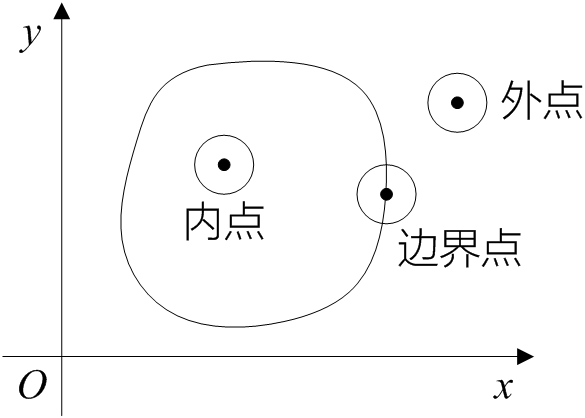
\includegraphics[height=3cm]{6.1.png}
\end{figure}

若$D$中每一个聚点都属于$D$,则称$D$为{\bf 闭集}。
若$D$中每个点都只是内点,称$D$为{\bf 开集}。
若开集$D$中任何两点均可用一条折线相连,则称为{\bf 连通的开集}或{\bf 开区域}。
开区域连同其边界称为{\bf 闭区域}。
对于点集$D$,若存在$M>0$,使得中任意两点的距离都小于$M$,称$D$为{\bf 有界区域},否则称为{\bf 无界区域}。
\end{definition}

这里,通过邻域的概念完整地定义了内点和外点,同时定义了边界点。
注意邻域概念的运用,对于内点外点,强调存在性,对于边界点,强调任一性。

最终要定义的是开区域和闭区域,类似一元函数中的开区间和闭区间,为此,需要首先定义各类点的概念和开集、闭集。

%============================================================
\subsection{二元数量值函数和二元向量值函数}

\begin{definition}[二元数量值函数]
设$D$为$\mathbb{R} ^2$的一个非空子集,$f$为$D\mapsto \mathbb{R} $的一个映射,对于$D$中的每一个矢量$\boldsymbol{p}$,$\mathbb{R} $中都有唯一的实数$z$与之对应,则称$f$为定义在$D$上的{\bf 二元数量值函数},也称{\bf 二元函数},写作:
\[
z=f\left( \boldsymbol{p} \right) \quad \boldsymbol{p}\in D
\]
其中$\boldsymbol{p}$称为{\bf 自变量},$z$称为{\bf 因变量},$D$称为{\bf 定义域}。
\end{definition}

二元数量值函数描述的是一个有序实数对到一个实数的映射:
\[
f:\boldsymbol{p}\mapsto z
\]
几何上可以用{\it xyz}直角坐标系描述。
$\boldsymbol{p}$表示平面{\it xy}平面上的点,$z$表示{\it z}轴上的值,$z=f\left( \boldsymbol{p} \right) $表示三维空间内的一个曲面。

\begin{definition}[二元向量值函数]
设$D$为$\mathbb{R} ^2$的一个非空子集,$\boldsymbol{f}$为$D\mapsto \mathbb{R} $的一个映射,对于$D$中的每一个矢量$\boldsymbol{p}$,$\mathbb{R} ^2$中都有唯一的实数$\boldsymbol{z}$与之对应,则称$\boldsymbol{f}$为定义在$D$上的{\bf 二元向量值函数},写作:
\[
\boldsymbol{z}=\boldsymbol{f}\left( \boldsymbol{p} \right) =\left( \begin{array}{c}
	P\left( \boldsymbol{p} \right)\\
	Q\left( \boldsymbol{p} \right)\\
\end{array} \right) \qquad \boldsymbol{p}\in D
\]
其中$\boldsymbol{p}$称为{\bf 自变量},$\boldsymbol{z}$称为{\bf 因变量},$D$称为{\bf 定义域},$P,Q$为$\boldsymbol{f}$对应的两个二元数量值函数。
\end{definition}

二元向量值函数描述的是一个有序实数到另一个有序实数对的映射:
\[
\boldsymbol{f}:\boldsymbol{p}\mapsto \boldsymbol{z}
\]
几何上比较难描述。

同样,可定义三维的向量值函数:
\[
\boldsymbol{z}=\boldsymbol{f}\left( \boldsymbol{p} \right) =\left( \begin{array}{c}
	P\left( \boldsymbol{p} \right)\\
	Q\left( \boldsymbol{p} \right)\\
	R\left( \boldsymbol{p} \right)\\
\end{array} \right) \qquad \boldsymbol{p}\in \mathbb{R} ^3
\]

%============================================================
\subsection{还是要光滑的}

一元函数微积分中,我们贯穿始终地考察光滑的曲线,二元函数也是一样。

学习二元函数微积分,我们可以将其与三维空间对应起来,用三维空间中的面和线,从几何角度理解二元函数微积分。
二元函数中我们喜欢的是光滑的面和线,同样需要对光滑进行定义。






\newpage
\section{极限}

本节讨论二元函数的极限。

本节要点:
\begin{itemize}
    \item 掌握极限的概念;
    \item 理解二元函数极限存在的要求。
\end{itemize}

%============================================================
\subsection{极限的概念}

\begin{definition}[极限]
设$z=f\left( \boldsymbol{p} \right) $为定义在$D$上的一个二元数量值函数,$\boldsymbol{p}_0$为$D$的聚点,如果对于$\forall \varepsilon >0$总存在$\delta >0$,使得当$0<\left\| \boldsymbol{p}-\boldsymbol{p}_0 \right\| <\delta $时,有$\left| z-A \right|<\varepsilon $,则称$A$为{\bf $f\left( \boldsymbol{p} \right) $当$\boldsymbol{p}\rightarrow \boldsymbol{p}_0$时的极限},记作$\underset{\boldsymbol{p}\rightarrow \boldsymbol{p}_0}{\lim}f\left( \boldsymbol{p} \right) $,即:
\[
\underset{\boldsymbol{p}\rightarrow \boldsymbol{p}_0}{\lim}f\left( \boldsymbol{p} \right) :=A
\]
\end{definition}

也即,对于无论什么给定多么小的$\varepsilon $,总能找到$\boldsymbol{p}_0$的一个去心邻域,使得该去心邻域内的所有矢量的函数值$z$和$A$的距离小于$\varepsilon $。
注意,这里必须是“去心”邻域。

%============================================================
\subsection{极限存在性的讨论}

二元函数中对于极限的要求是趋近方式(或称趋近方向)的任意性和趋近值的唯一性。
只要任何一条不满足,就不能说极限存在。
趋近方式的任意性要求,一般可以令$y=kx,k\in \mathbb{R} $或$y=k$或$x=k$,带入原式后简化看极限是否唯一,如果结果和$k$无关,说明满足趋近方式任意性。

这点同一元函数。
在一元函数中,左右极限均存在且相等$\Leftrightarrow $极限存在。
只是在二元函数中,“左右”两个方向变得复杂,变成了各个方向。

~

\begin{example}
设$\boldsymbol{p}=\left( x\,\,y \right) ^T$,若二元函数$f\left( \boldsymbol{p} \right) =\frac{xy}{x^2+y^2}$,讨论在原点处的极限是否存在。
\end{example}

解:

令$y=kx,k\in \mathbb{R} $表示任意方向,有:
\[
f\left( x,y \right) =\frac{kx^2}{x^2+k^2x^2}=\frac{k}{1+k^2}
\]
可见,不同的方向有不同的函数值,该二元函数在原点处不存在极限,该二元函数的图像:

\begin{figure}[ht]
\centering
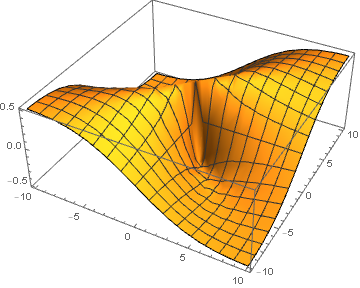
\includegraphics[height=4cm]{6.2.png}
\end{figure}

~

\begin{example}
设$\boldsymbol{p}=\left( x\,\,y \right) ^T$,若二元函数$f\left( \boldsymbol{p} \right) =\left( x^2+y^2 \right) e^{-\left( x^2+y^2 \right)}$,讨论在点$\left( -\infty ,+\infty \right) $处的极限是否存在。
\end{example}

解:

解法一,令$y=kx$表示任意方向,有:
\begin{align*}
    \underset{x\rightarrow -\infty ,y\rightarrow +\infty}{\lim}f\left( x,y \right) &=\underset{x\rightarrow -\infty ,y\rightarrow +\infty}{\lim}\left( x^2+k^2x^2 \right) e^{-\left( x^2+k^2x^2 \right)} \\
    &=\underset{x\rightarrow -\infty ,y\rightarrow +\infty}{\lim}\frac{\left( 1+k^2 \right) x^2}{e^{\left( 1+k^2 \right) x^2}} \\
    &=\underset{x\rightarrow -\infty ,y\rightarrow +\infty}{\lim}\frac{1}{e^{\left( 1+k^2 \right) x^2}} \\
    &=0
\end{align*}
极限存在且等于0。

解法二,点$\left( -\infty ,+\infty \right) $即为$\left\| \boldsymbol{p} \right\| \rightarrow \infty $:
\begin{align*}
&f\left( \boldsymbol{p} \right) =\left( x^2+y^2 \right) e^{-\left( x^2+y^2 \right)}=\left\| \boldsymbol{p} \right\| ^2e^{-\left\| \boldsymbol{p} \right\| ^2} \\
&\underset{\left\| \boldsymbol{p} \right\| ^2\rightarrow +\infty}{\lim}f\left( \boldsymbol{p} \right) =\underset{\left\| \boldsymbol{p} \right\| ^2\rightarrow +\infty}{\lim}\left\| \boldsymbol{p} \right\| ^2e^{-\left\| \boldsymbol{p} \right\| ^2}=0
\end{align*}






\newpage
\section{光滑曲面的第一个要求}

对于一个好的二元函数,我们的要求依然是“光滑”,同样要不断不折。

我们依然通过连续定义光滑的第一个要求——不断。
但是二元函数里,曲面的断复杂许多,其复杂性体现在方向的多元化。






\newpage
\section{连续}

本节讨论二元函数的连续。

本节要点:
\begin{itemize}
    \item 掌握连续的概念;
    \item 理解关于连续的定理和推论。
\end{itemize}

%============================================================
\subsection{连续的概念}

\begin{definition}[连续]
设二元数量值函数$z=f\left( \boldsymbol{p} \right) $的定义域为$D$,$\boldsymbol{p}_0$为$D$的聚点,且$\boldsymbol{p}_0\in D$,若满足
\[
\underset{\boldsymbol{p}\rightarrow \boldsymbol{p}_0}{\lim}f\left( \boldsymbol{p} \right) =f\left( \boldsymbol{p}_0 \right)
\]
则称{\bf $z=f\left( \boldsymbol{p} \right) $在$\boldsymbol{p}_0$处连续}。
反之,则称{\bf $z=f\left( \boldsymbol{p} \right) $在$\boldsymbol{p}_0$处不连续}。
不连续的点称为{\bf 间断点}。二元函数的间断点可以是孤立的点,也可以是一条或多条曲线。
\end{definition}

连续在数学上规范了什么是“不断”。
这个断不再是一元函数中简单的断点,而是需要各个方向看来不断。
虽然连续的定义从文字上和一元函数一样,但是具体判断起来要复杂得多。

%============================================================
\subsection{连续的定理}

\begin{theorem}[初等函数连续定理]
初等函数是指由常量及基本初等函数经过有限次四则运算与复合且能用一个式子表示的函数,一切二元初等函数在其定义区域内是连续的。
因此二元初等函数在其定义区域内的极限值就等于其函数值。
\end{theorem}

\begin{theorem}[最值定理]
若$z=f\left( \boldsymbol{p} \right) $在有界闭区域$D$连续,则必在$D$上有最大值和最小值。
\end{theorem}

\begin{theorem}[介值定理]
若$z=f\left( \boldsymbol{p} \right) $在有界闭区域$D$连续,且$f\left( \boldsymbol{p}_1 \right) \ne f\left( \boldsymbol{p}_2 \right) $,则对于$\forall \mu \in \left[ f\left( \boldsymbol{p}_1 \right) ,f\left( \boldsymbol{p}_2 \right) \right] $,必有$\boldsymbol{q}\in D$,使得$f\left( \boldsymbol{q} \right) =\mu $。
\end{theorem}

\begin{corollary}
若$z=f\left( \boldsymbol{p} \right) $在有界闭区域$D$连续,且有最大值和最小值$m,M$,则对于$\forall \mu \in \left[ M,m \right] $,必有$\boldsymbol{q}\in D$,使得$f\left( \boldsymbol{q} \right) =\mu $。
\end{corollary}

最值定理表达的是在有界闭区域连续的曲面必有界。
介值定理及其推论表达的是连续曲面任意两点间必有通路。






\newpage
\section{本章小结}

本章以二元函数为例讨论多元微积分的基础概念。
极限和连续的概念在二元函数均有所扩展。

要注意,极限在二元函数中比在一元函数中复杂很多。
一元函数中,极限存在的充分必要条件是左右极限都存在且相等。
二元函数中可以说类似,但要求的是各个方向的极限都存在且相等,这使得判断复杂很多,也困难很多。
连续的数学意义在于计算初等函数的极限,即,只要一个二元函数是“初等函数”,则在其定义域内任何点的极限都存在,都为该点的函数值。
注意,$f\left( \boldsymbol{p} \right) =\frac{xy}{x^2+y^2}$这种不是二元初等函数!

形而上来讲,我们开始了对高维空间几何体的“光滑”的考察。
本章是第一步,不断。






\newpage
\section{习题}

\begin{exercise}
计算下列极限:
\begin{enumerate}
    \item $\underset{x\rightarrow a,y\rightarrow 0}{\lim}\frac{\sin xy}{y}$
    \item $\underset{x,y\rightarrow 0}{\lim}\frac{x^2-y^2}{\sqrt{x-y+9}-3}$
    \item $\underset{x,y\rightarrow 0}{\lim}\frac{\ln \left[ 1+x\left( x^2+y^2 \right) \right]}{x^2+y^2}$
    \item $\underset{x,y\rightarrow 1/2}{\lim}\frac{\sin \left( x^2+2xy+y^2-1 \right)}{x+y-1}$
    \item $\underset{x\rightarrow 0,y\rightarrow 2}{\lim}\left( 1+xy \right) ^{\frac{1}{x}}$
    \item $\underset{x,y\rightarrow 0}{\lim}\left( x^2+y^2 \right) \sin \frac{1}{xy}$
    \item $\underset{x,y\rightarrow +\infty }{\lim}\left( x^2+y^2 \right) e^{-\left( x+y \right)}$
\end{enumerate}
\end{exercise}

解:

1.
\[
\underset{x\rightarrow a,y\rightarrow 0}{\lim}\frac{\sin xy}{y}=\underset{x\rightarrow a,y\rightarrow 0}{\lim}\frac{x\sin xy}{xy}=\underset{x\rightarrow a}{\lim}x=a
\]

2.
\begin{align*}
\underset{x,y\rightarrow 0}{\lim}\frac{x^2-y^2}{\sqrt{x-y+9}-3}&=\underset{x,y\rightarrow 0}{\lim}\frac{\left( x^2-y^2 \right) \cdot \left( \sqrt{x-y+9}+3 \right)}{x-y} \\
&=\underset{x,y\rightarrow 0}{\lim}\left( x+y \right) \cdot \left( \sqrt{x-y+9}+3 \right) =0
\end{align*}

3.
\begin{align*}
\underset{x,y\rightarrow 0}{\lim}\frac{\ln \left[ 1+x\left( x^2+y^2 \right) \right]}{x^2+y^2}&=\underset{x,y\rightarrow 0}{\lim}\ln \left[ 1+x\left( x^2+y^2 \right) \right] ^{\frac{1}{x^2+y^2}} \\
&=\underset{x,y\rightarrow 0}{\lim}\ln \left[ 1+x\left( x^2+y^2 \right) \right] ^{\frac{x}{x\left( x^2+y^2 \right)}} \\
&=\underset{x,y\rightarrow 0}{\lim}\ln e^x=\ln e^0=0
\end{align*}

4.
\begin{align*}
\underset{x,y\rightarrow 1/2}{\lim}\frac{\sin \left( x^2+2xy+y^2-1 \right)}{x+y-1}&=\underset{x,y\rightarrow 1/2}{\lim}\frac{\sin \left[ \left( x+y \right) ^2-1 \right]}{x+y-1} \\
&=\underset{u\rightarrow 1}{\lim}\frac{\sin \left( u^2-1 \right)}{u-1} \\
&=\underset{u\rightarrow 1}{\lim}\frac{\left( u+1 \right) \sin \left( u^2-1 \right)}{u^2-1}=2
\end{align*}

5.
\[
\underset{x\rightarrow 0,y\rightarrow 2}{\lim}\left( 1+xy \right) ^{\frac{1}{x}}=\underset{x\rightarrow 0,y\rightarrow 2}{\lim}\left( 1+xy \right) ^{\frac{y}{xy}}=\underset{y\rightarrow 2}{\lim}e^y=e^2
\]

6. 夹逼定理:
\begin{align*}
&\because -\left( x^2+y^2 \right) \leqslant \left( x^2+y^2 \right) \sin \frac{1}{xy}\leqslant x^2+y^2 \\
&\because \underset{x,y\rightarrow 0}{\lim}-\left( x^2+y^2 \right) =\underset{x,y\rightarrow 0}{\lim}\left( x^2+y^2 \right) =0 \\
&\therefore \underset{x,y\rightarrow 0}{\lim}\left( x^2+y^2 \right) \sin \frac{1}{xy}=0
\end{align*}

7. 夹逼定理:
\begin{align*}
&\because \left( x+y \right) e^{-\left( x+y \right)}<\left( x^2+y^2 \right) e^{-\left( x+y \right)}\leqslant \left( x+y \right) ^2e^{-\left( x+y \right)} \\
&\because \underset{x,y\rightarrow +\infty }{\lim}\left( x+y \right) e^{-\left( x+y \right)}=\underset{x,y\rightarrow +\infty }{\lim}\left( x+y \right) ^2e^{-\left( x+y \right)}=0 \\
&\therefore \underset{x,y\rightarrow +\infty }{\lim}\left( x^2+y^2 \right) e^{-\left( x+y \right)}=0
\end{align*}

\begin{tcolorbox}
本题总体思路是找到$x,y$的关系。
\end{tcolorbox}

~

\begin{exercise}
讨论下列函数在原点处的连续性:
\begin{enumerate}
    \item 
    $
    f\left( x,y \right) =\begin{cases}
        x\sin \frac{1}{x^2+y^2} & \left( x,y \right) \ne \left( 0,0 \right)\\
        0                       & \left( x,y \right) =\left( 0,0 \right)\\
    \end{cases}
    $
    \item 
    $
    f\left( x,y \right) =\begin{cases}
        \left( 1+x \right) ^{\frac{y}{x}} & x\ne 0\\
        e^y                               & x=0\\
    \end{cases}
    $
    \item 
    $
    f\left( x,y \right) =\begin{cases}
        \frac{x^2y}{x^4+y^2} & x^4+y^2\ne 0\\
        0                    & x^4+y^2=0\\
    \end{cases}
    $
\end{enumerate}
\end{exercise}

解:

1. 夹逼定理:
\begin{align*}
&\because -x<x\sin \frac{1}{x^2+y^2}\leqslant x \\
&\because \underset{x,y\rightarrow 0}{\lim}\left( -x \right) =\underset{x,y\rightarrow 0}{\lim}x=0 \\
&\therefore \underset{x,y\rightarrow 0}{\lim}x\sin \frac{1}{x^2+y^2}=0
\end{align*}

函数在原点处连续。

2.
\[
\underset{x,y\rightarrow 0}{\lim}\left( 1+x \right) ^{\frac{y}{x}}=\underset{y\rightarrow 0}{\lim}e^y
\]

函数在原点处连续。

3.
\[
\underset{x,y\rightarrow 0}{\lim}\frac{x^2y}{x^4+y^2}\overset{y=kx^2}{=}\underset{x\rightarrow 0}{\lim}\frac{kx^4}{x^4\left( 1+k \right)}
\]

极限不存在,所以函数在原点处不连续。

\begin{tcolorbox}
本题总体思路是计算原点处的极限。
\end{tcolorbox}










\chapter{多元函数微分学}

多元函数微分学与一元函数微分学一样,需要建立导数和微分。

一元函数在工程上基本以时间$t$为自变量,其变化无方向这个概念。
而多元函数不同,它有多个自变量,所以构成的变化量有方向这个概念。
所以多元函数导数讨论的是在一个特定方向上函数的变化率,即方向导数。

而研究与方向相关的变化率较为困难,所以先考察两个自变量方向上的变化率,即偏导。
将一元函数中的导数的概念和定理引入多元函数,再引出全微分,最后引出方向导数和梯度。

本章要点:
\begin{itemize}
    \item 偏导数。
    \item 方向导数。
    \item 全微分。
    \item 梯度。
\end{itemize}

~

\newpage
\section{光滑曲面的第二个要求}

光滑曲面的第二个要求是不折。

这里要捋清几个对应关系。
一元函数对应二维平面,对应{\it xy}直角坐标系,在二维平面中,光滑曲线的要求——不断不折,体现为连续和可导,由于可导和可微的等价性,也可以表现为连续和可微。
二元函数对应三维空间,对应{\it xyz}直角坐标系,在三维空间中,同样对光滑曲面有不折不断的要求,体现为连续和可微,这里的连续和可微都要求各个方向。

定义二元函数的导数是一件麻烦的事情。
首先,二元函数有两个变量,所以变化率会有沿着两个方向。
其次,如果我们考虑一个“总的变化率”,它的大小将随着方向的变化而变化,即总变化率是一个有方向的量,我们用矢量描述它将会比较合适。
综合下来,二元函数中没有“导数”这个概念,与一元函数导数对等的是一个叫“梯度”的概念。
梯度和可微是等价概念。更准确地讲,是一维空间中“导数”这个概念对应着多维空间中的“梯度”和“散度”两个概念。

\begin{table}[h]
\centering
\begin{tabular}{lll}
    \toprule
    概念 & 一元函数中的定义 & 二元函数中的定义\\
    \midrule
    极限        & $\underset{x\rightarrow x_0}{\lim}f\left( x \right) =A$ & $\underset{\boldsymbol{p}\rightarrow \boldsymbol{p}_0}{\lim}f\left( \boldsymbol{p} \right) =A$\\
    连续        & $\underset{x\rightarrow x_0}{\lim}f\left( x \right) =f\left( x_0 \right) $ & $\underset{\boldsymbol{p}\rightarrow \boldsymbol{p}_0}{\lim}f\left( \boldsymbol{p} \right) =f\left( \boldsymbol{p}_0 \right) $\\
    导数/梯度   & $\frac{dy}{dx}$ & $\nabla z=\left( \frac{\partial z}{\partial x}\,\,\frac{\partial z}{\partial y} \right) ^T$\\
    微分/全微分 & $dy=y'dx$ & $dz=\frac{\partial z}{\partial x}dx+\frac{\partial z}{\partial y}dy$\\
    偏导数      &  & $\frac{\partial z}{\partial x},\frac{\partial z}{\partial y}$\\
    方向导数    &  & $\frac{\partial z}{\partial n}=\frac{\partial z}{\partial x}\cos \alpha +\frac{\partial z}{\partial y}\cos \beta $\\
    \bottomrule
\end{tabular}
\end{table}

二元函数中,梯度和全微分都是建立在偏导数的基础上,所以本章先从偏导入手,再介绍全微分和梯度。






\newpage
\section{关于增量的记号}

本节我们先定义一些关于增量的记号。

本节要点:
\begin{itemize}
    \item 熟悉各种增量记号。
\end{itemize}

%============================================================
\subsection{自变量的增量}

\begin{definition}[自变量的增量]
设有一矢量$\boldsymbol{p}$,若它只沿{\it x}轴方向有增量$\Delta x$,此时产生的增量矢称为{\bf $\boldsymbol{p}$沿{\it x}轴方向的偏增量},记作$\Delta _x\boldsymbol{p}$,
同样地,若它只沿{\it y}轴方向有增量$\Delta y$,此时产生的增量矢称为{\bf $\boldsymbol{p}$沿{\it y}轴方向的偏增量},记作$\Delta _y\boldsymbol{p}$,
我们将这个两个偏增量的和称为{\bf 矢量$\boldsymbol{p}$的全增量},记作$\Delta \boldsymbol{p}$,即:
\begin{align*}
&\Delta \boldsymbol{p}=\Delta _x\boldsymbol{p}+\Delta _y\boldsymbol{p}=\Delta x\mathbf{i}+\Delta y\mathbf{j}=\left( \begin{array}{c}
	\Delta x\\
	0\\
\end{array} \right) +\left( \begin{array}{c}
	0\\
	\Delta y\\
\end{array} \right) =\left( \begin{array}{c}
	\Delta x\\
	\Delta y\\
\end{array} \right) \\
&\left\| \Delta \boldsymbol{p} \right\| =\sqrt{\left( \Delta x \right) ^2+\left( \Delta y \right) ^2}
\end{align*}
值得注意的是,$\Delta _x\boldsymbol{p},\Delta _y\boldsymbol{p},\Delta \boldsymbol{p}$依然是矢量。
若有方向$n$,其方向余弦记为$\mathbf{n}=\left( \cos \alpha \,\,\cos \beta \right) ^T$,我们将$\boldsymbol{p}$在方向$n$上的增量称为{\bf $\boldsymbol{p}$沿$n$的方向增量},记作$\Delta _n\boldsymbol{p}$。
\end{definition}

\begin{figure}[h]
\centering
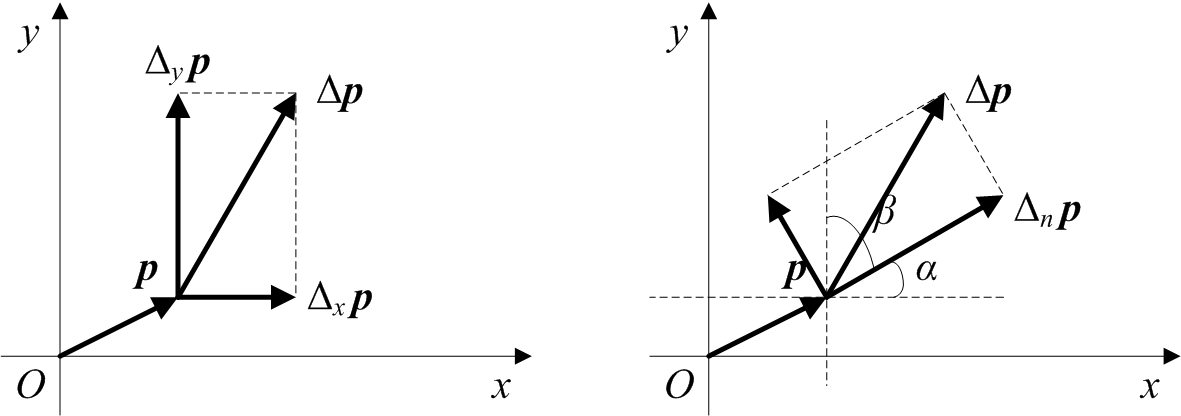
\includegraphics[height=3.5cm]{7.1.png}
\end{figure}

$\Delta _n\boldsymbol{p}$的表达式可以用坐标变换求得。
已知{\it xy}坐标系下的标准基及其构成的矩阵表示$A$:
\[
\boldsymbol{e}_1=\left( \begin{array}{c}
	1\\
	0\\
\end{array} \right) ,\boldsymbol{e}_2=\left( \begin{array}{c}
	0\\
	1\\
\end{array} \right) ,A=\left[ \begin{matrix}
	1&		0\\
	0&		1\\
\end{matrix} \right]
\]
新坐标系为原{\it xy}坐标系逆时针转$\alpha $,可得基及其构成的矩阵表示$W$:
\begin{align*}
&\because \begin{cases}
	L\left( \boldsymbol{e}_1 \right) =\left( \cos \alpha \,\,\sin \alpha \right) ^T\\
	L\left( \boldsymbol{e}_2 \right) =\left( -\sin \alpha \,\,\cos \alpha \right) ^T\\
\end{cases} \\
&\therefore W=\left[ \begin{matrix}
	\cos \alpha&		-\sin \alpha\\
	\sin \alpha&		\cos \alpha\\
\end{matrix} \right]
\end{align*}
由于:
\begin{align*}
&\because \Delta \boldsymbol{p}=A\left( \begin{array}{c}
	\Delta x\\
	\Delta y\\
\end{array} \right) =W\left( \begin{array}{c}
	\Delta n\\
	\Delta n_{\bot}\\
\end{array} \right) \\
&\therefore \left( \begin{array}{c}
	\Delta n\\
	\Delta n_{\bot}\\
\end{array} \right) =W^{-1}A\left( \begin{array}{c}
	\Delta x\\
	\Delta y\\
\end{array} \right) =\left( \begin{array}{c}
	\cos \alpha \Delta x+\sin \alpha \Delta y\\
	-\sin \alpha \Delta x+\cos \alpha \Delta y\\
\end{array} \right) \\
&\therefore \begin{cases}
	\Delta _n\boldsymbol{p}=\left( \begin{array}{c}
	\cos \alpha \Delta x+\sin \alpha \Delta y\\
	0\\
\end{array} \right)\\
	\Delta _{n_{\bot}}\boldsymbol{p}=\left( \begin{array}{c}
	0\\
	-\sin \alpha \Delta x+\cos \alpha \Delta y\\
\end{array} \right)\\
\end{cases}
\end{align*}
$\Delta _n\boldsymbol{p}$在{\it xy}坐标系下的表示:
\begin{align*}
&\because \Delta _n\boldsymbol{p}=A\left[ \Delta _n\boldsymbol{p} \right] _{xy}=W\left[ \Delta _n\boldsymbol{p} \right] _{nn_{\bot}}=W\left( \begin{array}{c}
	\cos \alpha \Delta x+\sin \alpha \Delta y\\
	0\\
\end{array} \right) \\
&\begin{aligned}
	\therefore \left[ \Delta _n\boldsymbol{p} \right] _{xy}&=\left[ \begin{matrix}
	\cos \alpha&		\sin \alpha\\
	-\sin \alpha&		\cos \alpha\\
\end{matrix} \right] \left( \begin{array}{c}
	\cos \alpha \Delta x+\sin \alpha \Delta y\\
	0\\
\end{array} \right)\\
    &=\left( \begin{array}{c}
	\cos \alpha \cos \alpha \Delta x+\sin \alpha \cos \alpha \Delta y\\
	-\sin \alpha \cos \alpha \Delta x-\sin \alpha \sin \alpha \Delta y\\
\end{array} \right)\\
	&=\left[ \begin{matrix}
	\cos \alpha \cos \alpha&		\sin \alpha \cos \alpha\\
	-\sin \alpha \cos \alpha&		-\sin \alpha \sin \alpha\\
\end{matrix} \right] \left( \begin{array}{c}
	\Delta x\\
	\Delta y\\
\end{array} \right)\\
	&=\left[ \begin{matrix}
	\cos \alpha \cos \alpha&		\cos \beta \cos \alpha\\
	-\cos \alpha \cos \beta&		-\cos \beta \cos \beta\\
\end{matrix} \right] \Delta \boldsymbol{p}\\
\end{aligned}
\end{align*}

\begin{tcolorbox}
这里需要重点弄清方向增量和全增量的关系。
\end{tcolorbox}

%============================================================
\subsection{因变量的增量}

\begin{definition}[因变量的增量]
若$z=f\left( \boldsymbol{p} \right) $,设开集$D$中的$\boldsymbol{p}$有偏增量$\Delta _x\boldsymbol{p},\Delta _y\boldsymbol{p}$,此时各自引起的$z$的增量称为{\bf 因变量$z$的偏增量},记为$\Delta _xz,\Delta _yz$,
同样地,若$\boldsymbol{p}$有全增量$\Delta \boldsymbol{p}$,则称引起的$z$的增量为{\bf 因变量$z$的全增量},记作$\Delta z$,
对应地,$\boldsymbol{p}$在$n$方向上的增量引起的$z$的增量称为{\bf 因变量$z$的方向增量},记作$\Delta _nz$,即:
\begin{align*}
&\Delta _xz=f\left( \boldsymbol{p}+\Delta _x\boldsymbol{p} \right) -f\left( \boldsymbol{p} \right) \\
&\Delta _yz=f\left( \boldsymbol{p}+\Delta _y\boldsymbol{p} \right) -f\left( \boldsymbol{p} \right) \\
&\Delta z=f\left( \boldsymbol{p}+\Delta \boldsymbol{p} \right) -f\left( \boldsymbol{p} \right) \\
&\Delta _nz=f\left( \boldsymbol{p}+\Delta _n\boldsymbol{p} \right) -f\left( \boldsymbol{p} \right)
\end{align*}
\end{definition}






\newpage
\section{偏导数和方向导数}

和一元函数一样,二元函数中我们也考察因变量对于自变量的变化率。
我们首先着重在一个维度(一个元)上考察函数的变化率——偏导,该概念用于引出后续的全微分、方向导数、梯度等概念,然后介绍方向导数,关于方向导数更多内容等讨论完全微分后继续深入。
本节着重理解偏导数的概念。

本节要点:
\begin{itemize}
    \item 掌握偏导数的定义;
    \item 了解二阶混偏相等定理;
    \item 了解方向导数的概念。
\end{itemize}

%============================================================
\subsection{偏导数的概念}

\begin{definition}[偏导数]
设函数$z=f\left( \boldsymbol{p} \right) $在点$\boldsymbol{p}_0$的某邻域内有定义,当$\boldsymbol{p}$有偏增量$\Delta _x\boldsymbol{p}$,相应地$z$也有偏增量$\Delta _xz$,如果$\Delta x\rightarrow 0$时,$\Delta _xz/\Delta x$的极限存在,则称此极限为{\bf 函数$z=f\left( \boldsymbol{p} \right) $在$\boldsymbol{p}_0$处对$x$的偏导数},记为$\left. \frac{\partial z}{\partial x} \right|_{\boldsymbol{p}_0}$,即:
\[
\left. \frac{\partial z}{\partial x} \right|_{\boldsymbol{p}_0}:=\underset{\Delta x\rightarrow 0}{\lim}\frac{\Delta _xz}{\Delta x}=\underset{\Delta x\rightarrow 0}{\lim}\frac{f\left( \boldsymbol{p}_0+\Delta _x\boldsymbol{p} \right) -f\left( \boldsymbol{p}_0 \right)}{\Delta x}
\]
也可记为$f_x\left( \boldsymbol{p}_0 \right) $。
同样定义$f_y\left( \boldsymbol{p}_0 \right) $,略。
\end{definition}

需要特别注意的是,偏导数是一个固定的实数。

\begin{definition}[偏导函数]
如果函数$z=f\left( \boldsymbol{p} \right) $在区域$D$内每一点,$\frac{\partial z}{\partial x},\frac{\partial z}{\partial y}
$存在,则称它们为{\bf $z=f\left( \boldsymbol{p} \right) $在区域$D$上的偏导函数},也可记为$f_x\left( \boldsymbol{p} \right) ,f_y\left( \boldsymbol{p} \right) $。
\end{definition}

除非特别指明,一般我们将偏导函数简称为偏导数。
需要特别注意的是,偏导函数依然是一个二元数量值函数。

由于偏导数只考虑一个变量,固定了其余所有变量,即把多元函数“退化”成一元函数,所以本质上偏导数还是一元函数中的导数。
偏导基于偏增量的概念——“固定一个,变动一个”,只要涉及偏导的定理,其证明过程都离不开偏增量概念。

二元函数极限的要求是“任意性”和“唯一性”。
而偏导数是固定了一个变量,变化另一个变化,缺乏了“任意性”,其次,二元函数在某点的各个偏导数不一定相同,缺乏“唯一性”,所以,函数在$\boldsymbol{p}_0$存在偏导数,并不能由此断定在该点存在极限,更不能断定在该点处连续。

%============================================================
\subsection{偏导数的几何意义}

对于二元函数$z=f\left( \boldsymbol{p} \right) $的偏导数$\frac{\partial z}{\partial x}$,由于固定了$y=y_0$,该函数变成了一元函数$z=f\left( x,y_0 \right) $。
几何上,是曲面$z=f\left( \boldsymbol{p} \right) $和平面$y=y_0$的交线。
偏导数的几何意义是曲线$z=f\left( x,y_0 \right) $在点$\boldsymbol{p}_0=\left( x_0\,\,y_0 \right) ^T$处的切线的斜率。

这里要注意,偏导的存在不能说明曲面是不折的,因为偏导相当于将曲面“切片”。
只是说明曲面在这个切片上投影出来的曲线是不折的。

%============================================================
\subsection{高阶偏导数的概念}

\begin{definition}[二阶偏导数]
设函数$z=f\left( \boldsymbol{p} \right) $在区域$D$内的两个偏导数$\frac{\partial z}{\partial x},\frac{\partial z}{\partial y}$都存在,进一步如果它们的偏导数也存在,则称这些偏导数是{\bf $z=f\left( \boldsymbol{p} \right) $的二阶偏导数},记为(二元函数一共4个二阶偏导):
\begin{align*}
&\frac{\partial}{\partial x}\left( \frac{\partial z}{\partial x} \right) =\frac{\partial ^2z}{\partial x^2}=f_{xx}\left( \boldsymbol{p} \right) \\
&\frac{\partial}{\partial y}\left( \frac{\partial z}{\partial x} \right) =\frac{\partial ^2z}{\partial x\partial y}=f_{xy}\left( \boldsymbol{p} \right) \\
&\frac{\partial}{\partial x}\left( \frac{\partial z}{\partial y} \right) =\frac{\partial ^2z}{\partial y\partial x}=f_{yx}\left( \boldsymbol{p} \right) \\
&\frac{\partial}{\partial y}\left( \frac{\partial z}{\partial y} \right) =\frac{\partial ^2z}{\partial y^2}=f_{yy}\left( \boldsymbol{p} \right)
\end{align*}
\end{definition}

\begin{theorem}[二阶混偏相等定理]
设函数$z=f\left( \boldsymbol{p} \right) $的两个二阶混合偏导数$\frac{\partial ^2z}{\partial x\partial y},\frac{\partial ^2z}{\partial y\partial x}$都存在,且这两个二阶混合偏导数都连续,则有
\[
\frac{\partial ^2z}{\partial x\partial y}=\frac{\partial ^2z}{\partial y\partial x}
\]
即:二阶混合偏导存在且均连续则有二阶偏导顺序无关。
\end{theorem}

%============================================================
\subsection{方向导数的概念}

\begin{definition}[方向导数]
设函数$z=f\left( \boldsymbol{p} \right) $在点$\boldsymbol{p}_0$的某邻域内有定义,由该点出发的一个方向$n$,在该方向上$\boldsymbol{p}$有方向增量$\Delta _n\boldsymbol{p}$,进而引起$z$产生方向增量$\Delta _nz$,若当$\left\| \Delta _n\boldsymbol{p} \right\| \rightarrow 0$时,$\frac{\Delta _nz}{\left\| \Delta _n\boldsymbol{p} \right\|}$存在极限,则称此极限为{\bf 函数$z=f\left( \boldsymbol{p} \right) $在点$\boldsymbol{p}_0$处沿方向$n$的方向偏导数},记作 ,即:
\[
\left. \frac{\partial z}{\partial n} \right|_{\boldsymbol{p}_0}:=\lim_{\left\| \Delta _n\boldsymbol{p} \right\| \rightarrow 0} \frac{\Delta _nz}{\left\| \Delta _n\boldsymbol{p} \right\|}=\lim_{\left\| \Delta _n\boldsymbol{p} \right\| \rightarrow 0} \frac{f\left( \boldsymbol{p}_0+\Delta _n\boldsymbol{p} \right) -f\left( \boldsymbol{p}_0 \right)}{\left\| \Delta _n\boldsymbol{p} \right\|}
\]
同样也有{\bf 方向导函数},记作$\frac{\partial z}{\partial n}$。
\end{definition}






\newpage
\section{全微分}

本节讨论全微分。
全微分是多元函数微分学的核心概念,是后续概念和定理的基础,同时在工程上也是一个用于估算微增量的非常有用的概念。

本节要点:
\begin{itemize}
    \item 掌握全微分定义;
    \item 深入理解全微分定理;
    \item 掌握全微分的应用。
\end{itemize}

%============================================================
\subsection{全微分的概念}

\begin{definition}[全微分]
如果区域$D$内有函数$z=f\left( \boldsymbol{p} \right) $,若在$\boldsymbol{p}_0\in D$处全增量满足:
\[
\Delta z=A\left( \boldsymbol{p}_0 \right) \Delta x+B\left( \boldsymbol{p}_0 \right) \Delta y+o\left( \left\| \Delta \boldsymbol{p} \right\| \right)
\]
其中:
\begin{itemize}
    \item $A\left( \boldsymbol{p}_0 \right) ,B\left( \boldsymbol{p}_0 \right) $:只与$\boldsymbol{p}_0$有关、与$\Delta \boldsymbol{p}$无关的常数;
    \item $\left\| \Delta \boldsymbol{p} \right\| $:自变量全增量$\Delta \boldsymbol{p}$的长度;
    \item $o\left( \left\| \Delta \boldsymbol{p} \right\| \right) $:当$\left\| \Delta \boldsymbol{p} \right\| \rightarrow 0$时,关于$\left\| \Delta \boldsymbol{p} \right\| $的高阶无穷小量,
\end{itemize}
则称{\bf 函数$z=f\left( \boldsymbol{p} \right) $在$\boldsymbol{p}_0$处可微},其中,$A\left( \boldsymbol{p}_0 \right) \Delta x+B\left( \boldsymbol{p}_0 \right) \Delta y$称为{\bf 全微分}(也称$\Delta z$的{\bf 线性主部}),记作$dz$,即:
\[
dz:=A\left( \boldsymbol{p}_0 \right) \Delta x+B\left( \boldsymbol{p}_0 \right) \Delta y
\]
如果函数在区域$D$内每点处都可微,则称{\bf 函数$z=f\left( \boldsymbol{p} \right) $在区域$D$内可微},由于$\Delta x=dx,\Delta y=dy$,上式也可写成:
\[
dz=A\left( \boldsymbol{p} \right) dx+B\left( \boldsymbol{p} \right) dy
\]
\end{definition}

%============================================================
\subsection{全微分的代数意义}

全微分表达的意思是,如果全增量$\Delta z$可以分成:
\begin{itemize}
    \item $A\Delta x+B\Delta y$:关于自变量偏增量的一个线性组合;
    \item $o\left( \left\| \Delta \boldsymbol{p} \right\| \right) $:可以忽略的无穷小量,
\end{itemize}
则认为$A\Delta x+B\Delta y$可以代替全增量$\Delta z$,即:
\[
\Delta z=A\Delta x+B\Delta y
\]

\begin{tcolorbox}
“线性化、以直代曲”是微分的目的,无论是多元函数全微分还是一元函数的微分。
\end{tcolorbox}

%============================================================
\subsection{全微分定理}

\begin{theorem}[全微分定理]
函数$z=f\left( \boldsymbol{p} \right) $可微$\Leftrightarrow $函数$z=f\left( \boldsymbol{p} \right) $连续且两个偏导数存在,且$A\left( \boldsymbol{p} \right) =\frac{\partial z}{\partial x},B\left( \boldsymbol{p} \right) =\frac{\partial z}{\partial y}$,即:
\[
dz=\frac{\partial z}{\partial x}dx+\frac{\partial z}{\partial y}dy
\]
\end{theorem}

\begin{proof}
该定理的关键点在于计算偏导$\frac{\partial z}{\partial x}$。
从可微和偏导各自的定义出发:
\begin{align*}
&\Delta z=A\left( \boldsymbol{p}_0 \right) \Delta x+B\left( \boldsymbol{p}_0 \right) \Delta y+o\left( \left\| \Delta \boldsymbol{p} \right\| \right) \\
&\left. \frac{\partial z}{\partial x} \right|_{\boldsymbol{p}_0}=\underset{\Delta x\rightarrow 0}{\lim}\frac{\Delta _xz}{\Delta x}=\underset{\Delta x\rightarrow 0}{\lim}\frac{f\left( \boldsymbol{p}_0+\Delta _x\boldsymbol{p} \right) -f\left( \boldsymbol{p}_0 \right)}{\Delta x}
\end{align*}
计算$\frac{\partial z}{\partial x}$如下:
\begin{align*}
&\left. \frac{\partial z}{\partial x} \right|_{\boldsymbol{p}_0}=\underset{\Delta x\rightarrow 0}{\lim}\frac{\Delta _xz}{\Delta x}=\underset{\Delta x\rightarrow 0}{\lim}\frac{f\left( \boldsymbol{p}_0+\Delta _x\boldsymbol{p} \right) -f\left( \boldsymbol{p}_0 \right)}{\Delta x} \\
&=\underset{\Delta x\rightarrow 0}{\lim}\frac{f\left( \boldsymbol{p}_0+\Delta _x\boldsymbol{p} \right) -f\left( \boldsymbol{p}_0 \right) +f\left( \boldsymbol{p}_0+\Delta \boldsymbol{p} \right) -f\left( \boldsymbol{p}_0+\Delta \boldsymbol{p} \right)}{\Delta x} \\
&=\underset{\Delta x\rightarrow 0}{\lim}\frac{\Delta z+f\left( \boldsymbol{p}_0+\Delta _x\boldsymbol{p} \right) -f\left( \boldsymbol{p}_0+\Delta \boldsymbol{p} \right)}{\Delta x} \\
&=\underset{\Delta x\rightarrow 0}{\lim}\frac{A\left( \boldsymbol{p}_0 \right) \Delta x+B\left( \boldsymbol{p}_0 \right) \Delta y+o\left( \left\| \Delta \boldsymbol{p} \right\| \right) +f\left( \boldsymbol{p}_0+\Delta _x\boldsymbol{p} \right) -f\left( \boldsymbol{p}_0+\Delta \boldsymbol{p} \right)}{\Delta x} \\
&=A\left( \boldsymbol{p}_0 \right) +\underset{\Delta x\rightarrow 0}{\lim}\frac{B\left( \boldsymbol{p}_0 \right) \Delta y-\left[ f\left( \boldsymbol{p}_0+\Delta \boldsymbol{p} \right) -f\left( \boldsymbol{p}_0+\Delta _x\boldsymbol{p} \right) \right] +o\left( \left\| \Delta \boldsymbol{p} \right\| \right)}{\Delta x}
\end{align*}
其中:
\begin{itemize}
    \item $B\left( \boldsymbol{p}_0 \right) \Delta y$:自变量的偏增量$\Delta y$引起的$z$从$\boldsymbol{p}_0$开始的线性部分增量;
    \item $f\left( \boldsymbol{p}_0+\Delta \boldsymbol{p} \right) -f\left( \boldsymbol{p}_0+\Delta _x\boldsymbol{p} \right) $:自变量的偏增量$\Delta y$引起的$z$从$\boldsymbol{p}_0+\Delta _x\boldsymbol{p}$开始的线性部分增量;
    \item $o\left( \left\| \Delta \boldsymbol{p} \right\| \right) $:当$\Delta x\rightarrow 0$时可以忽略的无穷小量。
\end{itemize}
当我们考察$\frac{\partial z}{\partial x}$时,有$\Delta y=0$,所以上述部分中前两部分的值为0,于是上式变为:
\[
\left. \frac{\partial z}{\partial x} \right|_{\boldsymbol{p}_0}=A\left( \boldsymbol{p}_0 \right) +\underset{\Delta x\rightarrow 0}{\lim}\frac{o\left( \left\| \Delta \boldsymbol{p} \right\| \right)}{\Delta x}=A\left( \boldsymbol{p}_0 \right)
\]
\end{proof}

一般函数偏导会存在,但函数本身不一定连续。
连续的前提条件是极限存在。
所以讨论多元函数在某点是否可微,首先得看该函数在该点的是否有极限,再看极限值是否为该函数值,即证明连续。
\begin{align*}
&\text{多元函数:可微} \Leftrightarrow \text{偏导} + \text{连续} \\
&\text{一元函数:可微} \Leftrightarrow \text{偏导} \Rightarrow \text{连续}
\end{align*}

%============================================================
\subsection{函数可微性的讨论}

函数在某点的可微性可从两个思路出发:

一、从微分的定义入手:
\begin{enumerate}
    \item 首先证明函数在该点的偏导数存在;
    \item 再证明余项$o\left( \left\| \Delta \boldsymbol{p} \right\| \right) $为$\left\| \Delta \boldsymbol{p} \right\| $的高阶无穷小量。
\end{enumerate}

二、从全微分定理入手:
\begin{enumerate}
    \item 同上,首先证明函数在该点的偏导数存在;
    \item 再证明函数在该点连续,即证明等式$\underset{\boldsymbol{p}\rightarrow \boldsymbol{p}_0}{\lim}f\left( \boldsymbol{p} \right) =f\left( \boldsymbol{p}_0 \right) $。
\end{enumerate}

~

\begin{example}
设函数$f\left( \boldsymbol{p} \right) =\left| x-y \right|g\left( \boldsymbol{p} \right) $,其中$g\left( \boldsymbol{p} \right) $在原点的某邻域内连续,问为$g\left( \mathbf{0} \right) $何值时$f\left( \boldsymbol{p} \right) $在原点处可微。
\end{example}

解一,从全微分定理入手。

首先考察偏导$f_x\left( \mathbf{0} \right) $对$g\left( \mathbf{0} \right) $的要求。
根据定义:
\[
\left. \frac{\partial f}{\partial x} \right|_{\mathbf{0}}=\underset{x\rightarrow 0}{\lim}\frac{\left| x \right|g\left( x,0 \right) -0\cdot g\left( x,0 \right)}{x-0}=\underset{x\rightarrow 0}{\lim}\frac{\left| x \right|g\left( x,0 \right)}{x}
\]
要使偏导存在,必须该极限存在,即左右极限存在且相等:
\[
\underset{x\rightarrow 0^+}{\lim}\frac{xg\left( x,0 \right)}{x}=\underset{x\rightarrow 0^-}{\lim}\frac{-xg\left( x,0 \right)}{x}
\]
由于$g\left( \boldsymbol{p} \right) $在原点的某邻域内连续,得到$g\left( \mathbf{0} \right) =0$,且有$\left. \frac{\partial f}{\partial x} \right|_{\mathbf{0}}=0$。对$f_y\left( \mathbf{0} \right) $分析,可得到同样结论。
考虑第二个条件——连续,根据定义,需要下式成立:
\[
\underset{x,y\rightarrow 0}{\lim}\left| x-y \right|g\left( x,y \right) =0
\]
由于刚才分析要求$g\left( \mathbf{0} \right) =0$,所以上式必然成立。
综合得到,当$g\left( \mathbf{0} \right) =0$时, 在原点处可微。

解二,从微分的定义出发证明无穷小量,即证明:
\begin{align*}
&\underset{\left\| \Delta \boldsymbol{p} \right\| \rightarrow 0}{\lim}\frac{o\left( \left\| \Delta \boldsymbol{p} \right\| \right)}{\left\| \Delta \boldsymbol{p} \right\|} \\
&=\underset{\left\| \Delta \boldsymbol{p} \right\| \rightarrow 0}{\lim}\frac{\left| \Delta x-\Delta y \right|g\left( \Delta x,\Delta y \right) -0\cdot g\left( 0,0 \right) -\frac{\partial f}{\partial x}\Delta x-\frac{\partial f}{\partial y}\Delta y}{\left\| \Delta \boldsymbol{p} \right\|}
\\
&=\underset{\Delta x,\Delta y\rightarrow 0}{\lim}\frac{\left| \Delta x-\Delta y \right|g\left( \Delta x,\Delta y \right)}{\sqrt{\Delta x^2+\Delta y^2}} \\
&\leqslant \underset{\Delta x,\Delta y\rightarrow 0}{\lim}\frac{\left| \Delta x \right|+\left| \Delta y \right|}{\sqrt{\Delta x^2+\Delta y^2}}g\left( \Delta x,\Delta y \right) \\
&\leqslant \sqrt{2}\cdot \underset{\Delta x,\Delta y\rightarrow 0}{\lim}g\left( \Delta x,\Delta y \right) \\
&=\sqrt{2}\cdot g\left( 0,0 \right) =0
\end{align*}
其中:
\begin{align*}
&\because \frac{\left| \Delta x \right|^2+\left| \Delta y \right|^2+2\left| \Delta x \right|\left| \Delta y \right|}{\left| \Delta x \right|^2+\left| \Delta y \right|^2}\leqslant \frac{\left| \Delta x \right|^2+\left| \Delta y \right|^2+\left| \Delta x \right|^2+\left| \Delta y \right|^2}{\left| \Delta x \right|^2+\left| \Delta y \right|^2}=2 \\
&\therefore \frac{\left| \Delta x \right|+\left| \Delta y \right|}{\sqrt{\left| \Delta x \right|^2+\left| \Delta y \right|^2}}\leqslant \sqrt{2}
\end{align*}

%============================================================
\subsection{全微分的应用——估值及误差}

同一元函数一样,用全微分我们可以近似计算一些工程值,不仅如此,我们还可以知道什么时候能做近似计算,以及误差是多少。
在做估算时,我们用$dz$代替$\Delta z$。
所以估算的关键是:
\begin{itemize}
    \item 构造合适的$f\left( \boldsymbol{p} \right) $,使得偏微分易于计算。
    \item 选定合适的$f\left( \boldsymbol{p}_0 \right) $,使得$\boldsymbol{p}_0$易于计算且对应的$\Delta x,\Delta y$非常小。
\end{itemize}

对于误差分析,我们定义如下概念:
\begin{itemize}
    \item {\bf 真值}:$f\left( \boldsymbol{p}_0+\Delta \boldsymbol{p} \right) $
    \item {\bf 绝对误差}:$\delta _z=\left| f_x\left( \boldsymbol{p}_0 \right) \right|\cdot dx+\left| f_y\left( \boldsymbol{p}_0 \right) \right|\cdot dy$
    \item {\bf 相对误差}:$\frac{\delta _z}{\left| z \right|}=\frac{\left| f_x\left( \boldsymbol{p}_0 \right) \right|\cdot dx+\left| f_y\left( \boldsymbol{p}_0 \right) \right|\cdot dy}{\left| z \right|}$
\end{itemize}

~

\begin{example}
求$1.04^{2.02}$近似值。
\end{example}

解:

首先构造一个合适的函数$z=f\left( \boldsymbol{p} \right) =x^y$,再选定起点$\boldsymbol{p}_0=\left( 1\,\,2 \right) ^T$,得:
\begin{align*}
1.04^{2.02}&\approx f\left( \boldsymbol{p}_0 \right) +dz \\
&=f\left( \boldsymbol{p}_0 \right) +f_x\left( \boldsymbol{p}_0 \right) \cdot dx+f_y\left( \boldsymbol{p}_0 \right) \cdot dy \\
&=1^2+\left. yx^{y-1} \right|_{\boldsymbol{p}_0}\cdot 0.04+\left. x^y\ln x \right|_{\boldsymbol{p}_0}\cdot 0.02 \\
&=1+0.08=1.08
\end{align*}
实际值是1.0824...,还是非常准的。


~

\begin{example}
如果我们通过电压电流测量计算电阻,已知电压表相对误差1\%,电流表相对误差0.5\%,如果测得电阻两端电压和电流分别为32V和8A,分析电阻的误差。
\end{example}

解:

电阻的绝对误差和相对误差:
\begin{align*}
&\delta _R=\left| f_V\left( V,I \right) \right|\cdot dV+\left| f_I\left( V,I \right) \right|\cdot dI=\left| \frac{1}{V} \right|dV+\left| -\frac{V}{I^2} \right|dI \\
&\frac{\delta _R}{\left| R \right|}=\frac{\delta _R}{\left| \frac{V}{I} \right|}
\end{align*}
电压电流的相对误差已知为1\%和0.5\%,可以计算它们的绝对误差:
\begin{align*}
&dV=32\cdot 1\% \\
&dI=8\cdot 0.5\%
\end{align*}
于是:
\begin{align*}
&\delta _R=\left| \frac{1}{V} \right|dV+\left| -\frac{V}{I^2} \right|dI=\frac{1}{8}\cdot \left( 32\cdot 1\% \right) +\frac{32}{8\cdot 8}\cdot \left( 8\cdot 0.5\% \right) =0.06\Omega \\
&\frac{\delta _R}{\left| R \right|}=\frac{\delta _R}{\left| \frac{V}{I} \right|}=\frac{0.06}{\left| \frac{32}{8} \right|}=15\%
\end{align*}






\newpage
\section{多元复合函数的求导}

对于多元复合函数,本节给出链式求导法则。

本节要点:
\begin{itemize}
    \item 掌握链式求导法则;
    \item 掌握引入中间变量转化为复合函数求解非初等多元函数的偏导;
    \item 掌握使用链式求导求解多元函数的高阶偏导;
    \item 了解雅可比矩阵和雅可比行列式。
\end{itemize}

%============================================================
\subsection{多元复合函数的概念}

\begin{definition}[复合函数]
设二元函数$z=z\left( u,v \right) $在某开集$D$有定义,又设$u=u\left( x,y \right) ,v=v\left( x,y \right) $在开集$E$内有定义,于是由$z,u,v$可构成一个{\bf 复合函数}:
\[
z=z\left( u\left( x,y \right) ,v\left( x,y \right) \right) \qquad \left( x,y \right) \in E
\]
\end{definition}

%============================================================
\subsection{多元复合函数的链式求导法则}

\begin{theorem}[链式求导法则]
对于复合函数$z=z\left( u\left( x,y \right) ,v\left( x,y \right) \right) $,若:
\begin{itemize}
    \item $u=u\left( x,y \right) ,v=v\left( x,y \right) $在点$\left( x,y \right) $处偏导存在;
    \item $z=z\left( u,v \right) $对应点$\left( u,v \right) $可微,
\end{itemize}
则$z=z\left( u\left( x,y \right) ,v\left( x,y \right) \right) $在点$\left( x,y \right) $处的偏导数存在,且有链式法则:
\begin{align*}
&\frac{\partial z}{\partial x}=\frac{\partial z}{\partial u}\cdot \frac{\partial u}{\partial x}+\frac{\partial z}{\partial v}\cdot \frac{\partial v}{\partial x} \\
&\frac{\partial z}{\partial y}=\frac{\partial z}{\partial u}\cdot \frac{\partial u}{\partial y}+\frac{\partial z}{\partial v}\cdot \frac{\partial v}{\partial y}
\end{align*}
\end{theorem}

证明略,关键是条件2不能减弱为$z=z\left( u,v \right) $在点$\left( u,v \right) $存在偏导。

~

三种特殊情况。

1、当有三个中间变量时,即$z=z\left( u,v,w \right) $,$u=u\left( x,y \right) $,$v=v\left( x,y \right) $,$w=w\left( x,y \right) $:
\begin{align*}
&\frac{\partial z}{\partial x}=\frac{\partial z}{\partial u}\cdot \frac{\partial u}{\partial x}+\frac{\partial z}{\partial v}\cdot \frac{\partial v}{\partial x}+\frac{\partial z}{\partial w}\cdot \frac{\partial w}{\partial x} \\
&\frac{\partial z}{\partial y}=\frac{\partial z}{\partial u}\cdot \frac{\partial u}{\partial y}+\frac{\partial z}{\partial v}\cdot \frac{\partial v}{\partial y}+\frac{\partial z}{\partial w}\cdot \frac{\partial w}{\partial y}
\end{align*}

2、当只有一个中间变量时,即$z=z\left( u \right) ,u=u\left( x,y \right) $:
\begin{align*}
&\frac{\partial z}{\partial x}=\frac{dz}{du}\cdot \frac{\partial u}{\partial x} \\
&\frac{\partial z}{\partial y}=\frac{dz}{du}\cdot \frac{\partial u}{\partial y}
\end{align*}

3、当只有一个自变量时,即$z=z\left( u,v \right) ,u=u\left( x \right) ,v=v\left( x \right) $,此时的$z$称为{\bf 一元复合函数}:
\[
\frac{dz}{dx}=\frac{\partial z}{\partial u}\cdot \frac{du}{dx}+\frac{\partial z}{\partial v}\cdot \frac{dv}{dx}
\]
该导数称为{\bf $z$对$x$的全导数}。

~

\begin{example}
设$z=\left( x^2+y^2 \right) ^{\sin \left( 2x+y \right)}$,求$\frac{\partial z}{\partial x}$。
\end{example}

解:

对于这类非初等函数,可以引入中间变量,令
\[
\begin{cases}
	u=x^2+y^2\\
	v=\sin \left( 2x+y \right)\\
\end{cases}
\]
则$z=u^v$,有:
\begin{align*}
\frac{\partial z}{\partial x}&=\frac{\partial z}{\partial u}\cdot \frac{\partial u}{\partial x}+\frac{\partial z}{\partial v}\cdot \frac{\partial v}{\partial x} \\
&=vu^{v-1}\cdot 2x+u^v\ln u\cdot 2\cos \left( 2x+y \right) \\
&=2x\cdot \sin \left( 2x+y \right) \cdot \left( x^2+y^2 \right) ^{\sin \left( 2x+y \right) -1} \\
& \quad +2\left( x^2+y^2 \right) ^{\sin \left( 2x+y \right)}\cdot \ln \left( x^2+y^2 \right) \cdot \cos \left( 2x+y \right)
\end{align*}

%============================================================
\subsection{雅可比矩阵和雅可比行列式}

对比一元函数的链式求导,复合函数$y=y\left( u\left( x \right) \right) $对$x$的求导:
\[
\frac{dy}{dx}=\frac{dy}{du}\cdot \frac{du}{dx}
\]
二元函数的链式求导能不能采用这种写法?

考察二元函数的链式求导,二元函数$z=z\left( u\left( x,y \right) ,v\left( x,y \right) \right) $在对$x,y$的偏导数为:
\begin{align*}
&\frac{\partial z}{\partial x}=\frac{\partial z}{\partial u}\cdot \frac{\partial u}{\partial x}+\frac{\partial z}{\partial v}\cdot \frac{\partial v}{\partial x} \\
&\frac{\partial z}{\partial y}=\frac{\partial z}{\partial u}\cdot \frac{\partial u}{\partial y}+\frac{\partial z}{\partial v}\cdot \frac{\partial v}{\partial y}
\end{align*}
采用矩阵方程的形式,可以写成:
\[
\left( \begin{array}{c}
	\frac{\partial z}{\partial x}\\
	\frac{\partial z}{\partial y}\\
\end{array} \right) =\left[ \begin{matrix}
	\frac{\partial u}{\partial x}&		\frac{\partial v}{\partial x}\\
	\frac{\partial u}{\partial y}&		\frac{\partial v}{\partial y}\\
\end{matrix} \right] \left( \begin{array}{c}
	\frac{\partial z}{\partial u}\\
	\frac{\partial z}{\partial v}\\
\end{array} \right)
\]

~

\begin{definition}
我们称由两个二元函数$u\left( x,y \right) ,v\left( x,y \right) $的四个一阶偏导数组成的矩阵称为这两个二元函数的{\bf 雅可比矩阵},即:
\[
\left[ \begin{matrix}
	\frac{\partial u}{\partial x}&		\frac{\partial u}{\partial y}\\
	\frac{\partial v}{\partial x}&		\frac{\partial v}{\partial y}\\
\end{matrix} \right]
\]
其对应的行列式称为{\bf 雅可比行列式},记为$\frac{\partial \left( u,v \right)}{\partial \left( x,y \right)}$,即;
\[
\frac{\partial \left( u,v \right)}{\partial \left( x,y \right)}=\left| \begin{matrix}
	\frac{\partial u}{\partial x}&		\frac{\partial u}{\partial y}\\
	\frac{\partial v}{\partial x}&		\frac{\partial v}{\partial y}\\
\end{matrix} \right|
\]
于是上式可以写为:
\[
\left( \begin{array}{c}
	\frac{\partial z}{\partial x}\\
	\frac{\partial z}{\partial y}\\
\end{array} \right) =\left[ \begin{matrix}
	\frac{\partial u}{\partial x}&		\frac{\partial u}{\partial y}\\
	\frac{\partial v}{\partial x}&		\frac{\partial v}{\partial y}\\
\end{matrix} \right] ^T\left( \begin{array}{c}
	\frac{\partial z}{\partial u}\\
	\frac{\partial z}{\partial v}\\
\end{array} \right)
\]
\end{definition}

同样可扩展三个三元函数$u\left( x,y,z \right) ,v\left( x,y,z \right) ,w\left( x,y,z \right) $的九个一阶偏导数组成的雅可比矩阵:
\[
\left[ \begin{matrix}
	\frac{\partial u}{\partial x}&		\frac{\partial u}{\partial y}&		\frac{\partial u}{\partial z}\\
	\frac{\partial v}{\partial x}&		\frac{\partial v}{\partial y}&		\frac{\partial v}{\partial z}\\
	\frac{\partial w}{\partial x}&		\frac{\partial w}{\partial y}&		\frac{\partial w}{\partial z}\\
\end{matrix} \right]
\]

对于雅可比行列式,有如下法则:
\begin{align*}
&\frac{\partial \left( u,v \right)}{\partial \left( x,y \right)}=\frac{\partial \left( u,v \right)}{\partial \left( s,t \right)}\cdot \frac{\partial \left( s,t \right)}{\partial \left( x,y \right)} \\
&\frac{\partial \left( u,v \right)}{\partial \left( x,y \right)}\cdot \frac{\partial \left( x,y \right)}{\partial \left( u,v \right)}=1 \\
&\frac{\partial \left( u,v \right)}{\partial \left( x,y \right)}=-\frac{\partial \left( v,u \right)}{\partial \left( x,y \right)} \\
&\frac{\partial \left( u,u \right)}{\partial \left( x,y \right)}=0
\end{align*}






\newpage
\section{隐函数的求导}

对于隐函数,本节给出隐函数的求偏导的方法,该方法去除了链式求导步骤,大大简化计算过程。
隐函数求导法在曲线积分和曲面积分中有重要使用,需要熟练掌握。

本节要点:
\begin{itemize}
    \item 掌握一元隐函数和二元隐函数的求导法则。
\end{itemize}

%============================================================
\subsection{一元隐函数的求导}

\begin{theorem}[一元隐函数求导定理]
将方程$F\left( x,y \right) =0$的左边看成二元函数$z=F\left( \boldsymbol{p} \right) $,若满足:
\begin{itemize}
    \item 在点$\boldsymbol{p}_0$的某一邻域内有连续的偏导数,且$\left. \frac{\partial z}{\partial y} \right|_{\boldsymbol{p}_0}\ne 0$,
    \item 点$\boldsymbol{p}_0$满足方程$F\left( \boldsymbol{p}_0 \right) =0$,
\end{itemize}
则点$\boldsymbol{p}_0$的某一邻域内,方程$F\left( x,y \right) =0$将唯一确定单值连续函数$y=y\left( x \right) $,使得$F\left( x,y\left( x \right) \right) =0$,且$y_0=y\left( x_0 \right) $,并有:
\[
\frac{dy}{dx}=-\frac{\frac{\partial z}{\partial x}}{\frac{\partial z}{\partial y}}=-\frac{F_x}{F_y}
\]
\end{theorem}

%============================================================
\subsection{二元隐函数的求导}

\begin{theorem}[二元隐函数求导定理]
将方程$F\left( x,y,z \right) =0$的左边看成三元函数$u=F\left( \boldsymbol{p} \right) ,\boldsymbol{p}=\left( x\,\,y\,\,z \right) ^T$,若满足:
\begin{itemize}
    \item 在点$\boldsymbol{p}_0$的某一邻域内有连续的偏导数,且$\left. \frac{\partial u}{\partial z} \right|_{\boldsymbol{p}_0}\ne 0$,
    \item 点$\boldsymbol{p}_0$满足方程$F\left( \boldsymbol{p}_0 \right) =0$,
\end{itemize}
则点$\boldsymbol{p}_0$的某一邻域内,方程$F\left( x,y,z \right) =0$将唯一确定单值连续函数$z=z\left( x,y \right) $,使得$F\left( x,y,z\left( x,y \right) \right) =0$,且$z_0=z\left( x_0,y_0 \right) $,并有:
\begin{align*}
&\frac{\partial z}{\partial x}=-\frac{\frac{\partial u}{\partial x}}{\frac{\partial u}{\partial z}}=-\frac{F_x}{F_z} \\
&\frac{\partial z}{\partial y}=-\frac{\frac{\partial u}{\partial y}}{\frac{\partial u}{\partial z}}=-\frac{F_y}{F_z}
\end{align*}
\end{theorem}

使用隐函数的求导方法时,首先创建一个函数$u=F\left( \boldsymbol{p} \right) $,此时,$z$再不是应变量,而是自变量。

~

\begin{example}
设$x^2+y^2+z^2=1$,求$\frac{\partial ^2z}{\partial x^2}$。
\end{example}

解:

令$u=F\left( x,y,z \right) =x^2+y^2+z^2-1$,可得:
\[
\frac{\partial z}{\partial x}=-\frac{F_x}{F_z}=-\frac{x}{z}
\]
继续求偏导:
\[
\frac{\partial ^2z}{\partial x^2}=\frac{\partial}{\partial x}\left( -\frac{x}{z} \right) =-\frac{z-x\frac{\partial z}{\partial x}}{z^2}=-\frac{z+x\frac{x}{z}}{z^2}
\]

~

\begin{example}
    设$x^2+y^2+z^2=yf\left( \frac{z}{y} \right) $,其中$f\left( u \right) $对$u$可微,求$\frac{\partial z}{\partial y}$。
\end{example}

解:

令$u=F\left( x,y,z \right) =x^2+y^2+z^2-yf\left( \frac{z}{y} \right) $,可得:
\[
\frac{\partial z}{\partial y}=-\frac{F_y}{F_z}=-\frac{2y-f\left( \frac{z}{y} \right) -yf'\left( \frac{z}{y} \right) \left( -\frac{z}{y^2} \right)}{2z-yf'\left( \frac{z}{y} \right) \frac{1}{y}}=-\frac{2y-f+\frac{z}{y}f'}{2z-f'}
\]

%============================================================
\subsection{方程组的求导}

上面提到的是一个三元方程$F\left( x,y,z \right) =0$确定的一个二元函数。
如果是两个四元方程组成的方程组,如下:
\[
\left\{ \begin{array}{c}
	F\left( x,y,u,v \right) =0\\
	G\left( x,y,u,v \right) =0\\
\end{array} \right.
\]
也可以确定两个二元函数$u=u\left( x,y \right) ,v=v\left( x,y \right) $。
以求$\frac{\partial u}{\partial x},\frac{\partial v}{\partial x}$为例,将两个方程两边分别对$x$求偏导:
\[
\begin{cases}
	\frac{\partial F}{\partial x}+\frac{\partial F}{\partial u}\cdot \frac{\partial u}{\partial x}+\frac{\partial F}{\partial v}\cdot \frac{\partial v}{\partial x}=0\\
	\frac{\partial G}{\partial x}+\frac{\partial G}{\partial u}\cdot \frac{\partial u}{\partial x}+\frac{\partial G}{\partial v}\cdot \frac{\partial v}{\partial x}=0\\
\end{cases}
\]
其实就是解一个二元一次方程组,化为矩阵形式:
\[
\left[ \begin{matrix}
	\frac{\partial F}{\partial u}&		\frac{\partial F}{\partial v}\\
	\frac{\partial G}{\partial u}&		\frac{\partial G}{\partial v}\\
\end{matrix} \right] \cdot \left( \begin{array}{c}
	\frac{\partial u}{\partial x}\\
	\frac{\partial u}{\partial y}\\
\end{array} \right) =-\left( \begin{array}{c}
	\frac{\partial F}{\partial x}\\
	\frac{\partial G}{\partial y}\\
\end{array} \right)
\]
解用雅可比行列式可以写成:
\[
\begin{cases}
	\frac{\partial u}{\partial x}=-\frac{\partial \left( F,G \right)}{\partial \left( x,v \right)}/\frac{\partial \left( F,G \right)}{\partial \left( u,v \right)}\\
	\frac{\partial v}{\partial x}=-\frac{\partial \left( F,G \right)}{\partial \left( u,x \right)}/\frac{\partial \left( F,G \right)}{\partial \left( u,v \right)}\\
\end{cases}
\]

~

\begin{example}
若方程组
\[
\begin{cases}
	u^3+xv-y=0\\
	v^3+yu-x=0\\
\end{cases}
\]
可确定的函数$u=u\left( x,y \right) ,v=v\left( x,y \right) $,求偏导数$\frac{\partial u}{\partial x},\frac{\partial v}{\partial x}$。
\end{example}

解:

用上面的方法,直接写出解的公式:
\begin{align*}
&\frac{\partial \left( F,G \right)}{\partial \left( x,v \right)}=\left| \begin{matrix}
	\frac{\partial F}{\partial x}&		\frac{\partial F}{\partial v}\\
	\frac{\partial G}{\partial x}&		\frac{\partial G}{\partial v}\\
\end{matrix} \right|=v\cdot 3v^2-x\cdot \left( -1 \right) =x+3v^3 \\
&\frac{\partial \left( F,G \right)}{\partial \left( u,x \right)}=\left| \begin{matrix}
	\frac{\partial F}{\partial u}&		\frac{\partial F}{\partial x}\\
	\frac{\partial G}{\partial u}&		\frac{\partial G}{\partial x}\\
\end{matrix} \right|=3u^2\cdot \left( -1 \right) -v\cdot y=-vy-3u^2 \\
&\frac{\partial \left( F,G \right)}{\partial \left( u,v \right)}=\left| \begin{matrix}
	\frac{\partial F}{\partial u}&		\frac{\partial F}{\partial v}\\
	\frac{\partial G}{\partial u}&		\frac{\partial G}{\partial v}\\
\end{matrix} \right|=3u^2\cdot 3v^2-x\cdot y=9u^2v^2-xy
\end{align*}
解得:
\[
\begin{cases}
	\frac{\partial u}{\partial x}=-\frac{\partial \left( F,G \right)}{\partial \left( x,v \right)}/\frac{\partial \left( F,G \right)}{\partial \left( u,v \right)}=-\frac{x+3v^3}{9u^2v^2-xy}\\
	\frac{\partial v}{\partial x}=-\frac{\partial \left( F,G \right)}{\partial \left( u,x \right)}/\frac{\partial \left( F,G \right)}{\partial \left( u,v \right)}=-\frac{-vy-3u^2}{9u^2v^2-xy}\\
\end{cases}
\]



\newpage
\section{全微分的几何意义}

本节是对矢量、全微分和隐函数求导的汇总型应用,是空间矢量和微分的第一次结合,熟练掌握和细品。

本节要点:
\begin{itemize}
    \item 深入理解全微分的几何意义;
    \item 深入理解方向导数的概念。
\end{itemize}

%============================================================
\subsection{空间曲线的切线和法平面}

\begin{figure}[h]
\centering
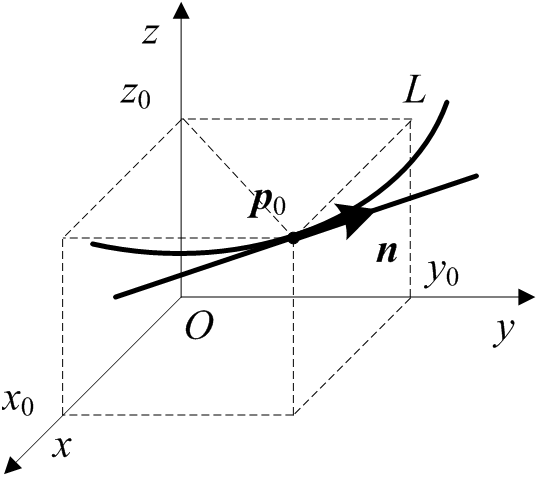
\includegraphics[height=4cm]{7.2.png}
\end{figure}

\begin{definition}
设三维空间的曲线
\[
L:\left\{ \begin{array}{c}
	x=x\left( t \right)\\
	y=y\left( t \right)\\
	z=z\left( t \right)\\
\end{array} \right.
\]
则曲线在点$\boldsymbol{p}_0$处(即对应$t_0$)的切线的方向称为{\bf 曲线$L$的切向量},假设记为$\boldsymbol{n}$,则有:
\[
\boldsymbol{n}=\left. \left( \begin{array}{c}
	x'\\
	y'\\
	z'\\
\end{array} \right) \right|_{t=t_0}=\left( \begin{array}{c}
	x'\left( t_0 \right)\\
	y'\left( t_0 \right)\\
	z'\left( t_0 \right)\\
\end{array} \right)
\]
于是,曲线$L$在点$\boldsymbol{p}_0$处的切线方程为$\boldsymbol{p}-\boldsymbol{p}_0=\lambda \boldsymbol{n}$,展开后为:
\[
\left( \begin{array}{c}
	x\\
	y\\
	z\\
\end{array} \right) -\left( \begin{array}{c}
	x_0\\
	y_0\\
	z_0\\
\end{array} \right) =\lambda \left( \begin{array}{c}
	x'\left( t_0 \right)\\
	y'\left( t_0 \right)\\
	z'\left( t_0 \right)\\
\end{array} \right) \quad \text{或} \quad \frac{x-x_0}{x'\left( t_0 \right)}=\frac{y-y_0}{y'\left( t_0 \right)}=\frac{z-z_0}{z'\left( t_0 \right)}
\]
过点$\boldsymbol{p}_0$垂直于该点切线的平面称为{\bf 曲线$L$在点$\boldsymbol{p}_0$处的法平面},法平面方程为$\left( \boldsymbol{p}-\boldsymbol{p}_0 \right) ^T\boldsymbol{n}=0$,展开后为:
\[
\left( x-x_0 \right) \cdot x'\left( t_0 \right) +\left( y-y_0 \right) \cdot y'\left( t_0 \right) +\left( z-z_0 \right) \cdot z'\left( t_0 \right) =0
\]
\end{definition}

如果曲线由两个平面
\[
L:\left\{ \begin{array}{c}
	F\left( x,y,z \right) =0\\
	G\left( x,y,z \right) =0\\
\end{array} \right.
\]
相交而成,则在点$\boldsymbol{p}_0$处的切向量为:
\[
\boldsymbol{n}=\left. \left( 1\,\,\frac{\partial y}{\partial x}\,\,\frac{\partial z}{\partial x} \right) ^T \right|_{\boldsymbol{p}_0}
\]
切线方程为:
\[
\frac{x-x_0}{1}=\frac{y-y_0}{\left. \frac{\partial y}{\partial x} \right|_{\boldsymbol{p}_0}}=\frac{z-z_0}{\left. \frac{\partial z}{\partial x} \right|_{\boldsymbol{p}_0}}
\]
法平面方程为:
\[
\left( x-x_0 \right) +\left( y-y_0 \right) \cdot \left. \frac{\partial y}{\partial x} \right|_{\boldsymbol{p}_0}+\left( z-z_0 \right) \cdot \left. \frac{\partial z}{\partial x} \right|_{\boldsymbol{p}_0}=0
\]

%============================================================
\subsection{空间曲面的切平面和法线}

\begin{figure}[h]
\centering
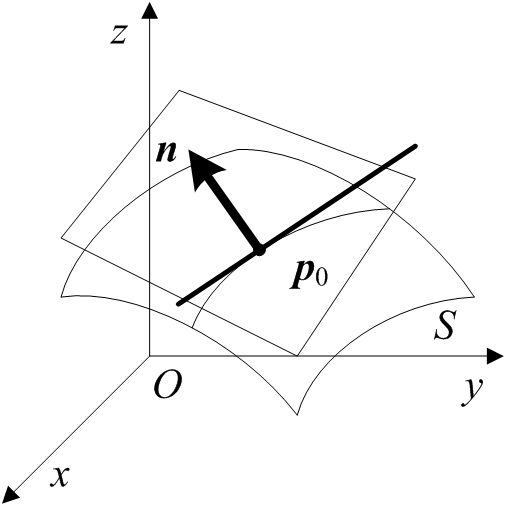
\includegraphics[height=4cm]{7.3.png}
\end{figure}

\begin{definition}
若曲面$S$由方程$F\left( \boldsymbol{p} \right) =0,\boldsymbol{p}=\left( x\,\,y\,\,z \right) ^T$隐式给出,对于在点$\boldsymbol{p}_0$处垂直于切平面的方向称为{\bf 曲面$S$在$\boldsymbol{p}_0$处的法向量},假设记为$\boldsymbol{n}$,则有:
\[
\boldsymbol{n}=\left. \left( \begin{array}{c}
	F_x\\
	F_y\\
	F_z\\
\end{array} \right) \right|_{\boldsymbol{p}_0}
\]
{\bf 曲面$S$在点$\boldsymbol{p}_0$处的法线方程}为$\boldsymbol{p}-\boldsymbol{p}_0=\lambda \boldsymbol{n}$,即:
\[
\left( \begin{array}{c}
	x\\
	y\\
	z\\
\end{array} \right) -\left( \begin{array}{c}
	x_0\\
	y_0\\
	z_0\\
\end{array} \right) =\lambda \left( \begin{array}{c}
	F_x\left( \boldsymbol{p}_0 \right)\\
	F_y\left( \boldsymbol{p}_0 \right)\\
	F_z\left( \boldsymbol{p}_0 \right)\\
\end{array} \right) \quad \text{或} \quad \frac{x-x_0}{F_x\left( \boldsymbol{p}_0 \right)}=\frac{y-y_0}{F_y\left( \boldsymbol{p}_0 \right)}=\frac{z-z_0}{F_z\left( \boldsymbol{p}_0 \right)}
\]
{\bf 曲面$S$在点$\boldsymbol{p}_0$处的切平面方程}为$\left( \boldsymbol{p}-\boldsymbol{p}_0 \right) ^T\boldsymbol{n}=0$,即:
\[
\left( x-x_0 \right) \cdot F_x\left( \boldsymbol{p}_0 \right) +\left( y-y_0 \right) \cdot F_y\left( \boldsymbol{p}_0 \right) +\left( z-z_0 \right) \cdot F_z\left( \boldsymbol{p}_0 \right) =0
\]
\end{definition}

若曲面由$z=z\left( x,y \right) $显式给出,则法向量:
\[
\boldsymbol{n}=\left. \left( \begin{array}{c}
	-z_x\\
	-z_y\\
	1\\
\end{array} \right) \right|_{\boldsymbol{p}_0}
\]
法线方程:
\[
\frac{x-x_0}{-z_x\left( \boldsymbol{p}_0 \right)}=\frac{y-y_0}{-z_y\left( \boldsymbol{p}_0 \right)}=\frac{z-z_0}{1}
\]
切平面方程:
\[
-\left( x-x_0 \right) \cdot z_x\left( \boldsymbol{p}_0 \right) -\left( y-y_0 \right) \cdot z_y\left( \boldsymbol{p}_0 \right) +\left( z-z_0 \right) =0
\]

~

\begin{example}
求曲面$x^2+2y^2+3z^2=6$在$\boldsymbol{p}_0=\left( 1\,\,1\,\,1 \right) $处的切平面和法线。
\end{example}

解:

构造$F=x^2+2y^2+3z^2-6$,得$\boldsymbol{p}_0$处的法线方向:
\[
\boldsymbol{n}=\left. \left( \begin{array}{c}
	F_x\\
	F_y\\
	F_z\\
\end{array} \right) \right|_{\boldsymbol{p}_0}=\left. \left( \begin{array}{c}
	2x\\
	4y\\
	6z\\
\end{array} \right) \right|_{\boldsymbol{p}_0}=\left( \begin{array}{c}
	2\\
	4\\
	6\\
\end{array} \right)
\]
切平面和法线:
\begin{align*}
&2\left( x-1 \right) +4\left( y-1 \right) +6\left( z-1 \right) =0 \\
&\frac{x-1}{2}=\frac{y-1}{4}=\frac{z-1}{6}
\end{align*}

%============================================================
\subsection{全微分的几何意义}

根据上节的空间曲面$z=z\left( x,y \right) $的切平面方程,对比全微分,如下:
\begin{align*}
&-\left( x-x_0 \right) \cdot z_x\left( \boldsymbol{p}_0 \right) -\left( y-y_0 \right) \cdot z_y\left( \boldsymbol{p}_0 \right) +\left( z-z_0 \right) =0 \\
&dz=z_x\cdot dx+z_y\cdot dy
\end{align*}
$z=z\left( x,y \right) $在点$\boldsymbol{p}_0$处的全微分的几何意义表示曲面$S$在点$\boldsymbol{p}_0$处的切平面在{\it z}轴的增量。

全微分的几何意义体现出一点,曲面要在某一点有切平面,必须在这一点光滑——不断不折。
只有光滑了,才有切平面,才有切平面在{\it z}轴的增量。
细品!

%============================================================
\subsection{方向导数定理}

我们之前定义了方向导数
\[
\left. \frac{\partial z}{\partial n} \right|_{\boldsymbol{p}_0}=\underset{\left\| \Delta _n\boldsymbol{p} \right\| \rightarrow 0}{\lim}\frac{\Delta _nz}{\left\| \Delta _n\boldsymbol{p} \right\|}=\underset{\left\| \Delta _n\boldsymbol{p} \right\| \rightarrow 0}{\lim}\frac{f\left( \boldsymbol{p}_0+\Delta _n\boldsymbol{p} \right) -f\left( \boldsymbol{p}_0 \right)}{\left\| \Delta _n\boldsymbol{p} \right\|}
\]
但当时还没有引入全微分,我们这里用全微分完善方向导数。

\begin{theorem}[方向导数定理]
设函数$z=z\left( \boldsymbol{p} \right) $在一点处可微,则该函数在此点处存在沿任意方向$n$的方向导数,且有:
\[
\frac{\partial z}{\partial n}=\frac{\partial z}{\partial x}\cos \alpha +\frac{\partial z}{\partial y}\cos \beta
\]
其中,$\mathbf{n}=\left( \cos \alpha \,\,\cos \beta \right) ^T$为方向$n$的方向余弦。
\end{theorem}

该定理给方向导数的计算提供了方法,即如果知道一个方向,就能知道沿该方向的方向导数。

同样,对于三元函数$u=u\left( \boldsymbol{p} \right) ,\boldsymbol{p}\in \mathbb{R} ^3$,方向导数为:
\[
\frac{\partial u}{\partial n}=\frac{\partial u}{\partial x}\cos \alpha +\frac{\partial u}{\partial y}\cos \beta +\frac{\partial u}{\partial z}\cos \gamma
\]

~

\begin{example}
求函数$z=xe^{2y}$在点$\boldsymbol{p}_0=\left( 1\,\,0 \right) ^T$处,沿射线$\left( 1\,\,0 \right) ^T\rightarrow \left( 2\,\,-1 \right) ^T$的方向导数。
\end{example}

解:

首先求得偏导:
\[
\left. \left( \frac{\partial z}{\partial x}\,\,\frac{\partial z}{\partial y} \right) ^T \right|_{\boldsymbol{p}_0}=\left. \left( e^{2y} \quad 2xe^{2y} \right) ^T \right|_{\boldsymbol{p}_0}=\left( 1\,\,2 \right) ^T
\]
再求射线的方向余弦:
\begin{align*}
&\because \Delta _n\boldsymbol{p}=\left( \begin{array}{c}
	2\\
	-1\\
\end{array} \right) -\left( \begin{array}{c}
	1\\
	0\\
\end{array} \right) =\left( \begin{array}{c}
	1\\
	-1\\
\end{array} \right)
\\
&\therefore \left\| \Delta _n\boldsymbol{p} \right\| =\sqrt{2} \\
&\therefore \mathbf{\theta }=\left( \frac{1}{\sqrt{2}}\,\,\frac{-1}{\sqrt{2}} \right) ^T
\end{align*}
最终,方向导数:
\[
\left. \frac{\partial z}{\partial n} \right|_{\boldsymbol{p}_0}=\left( 1\,\,2 \right) \left( \frac{1}{\sqrt{2}}\,\,\frac{-1}{\sqrt{2}} \right) ^T=\frac{1}{\sqrt{2}}+\frac{-2}{\sqrt{2}}=-\frac{1}{\sqrt{2}}
\]






\newpage
\section{梯度}

通过方向导数我们可以看到,若一个函数可微则任何方向的导数可以分解为两个偏导的线性组合,于是偏导可以认为是一个坐标系。
本节将这个概念定义化。

本节要点:
\begin{itemize}
    \item 掌握梯度的概念;
    \item 理解梯度的几何意义;
    \item 理解微分算子的概念。
\end{itemize}

%============================================================
\subsection{梯度的概念}

\begin{definition}[梯度]
设函数$z=z\left( \boldsymbol{p} \right) $在一点处可微,则称其两个偏导构成的矢量$\left( \frac{\partial z}{\partial x}\,\,\frac{\partial z}{\partial y} \right) ^T$为{\bf $z=z\left( \boldsymbol{p} \right) $在该点处的梯度},记为$\mathbf{grad}z$,简记为$\nabla z$,即:
\[
\nabla z:=\left( \begin{array}{c}
	\frac{\partial z}{\partial x}\\
	\frac{\partial z}{\partial y}\\
\end{array} \right)
\]
\end{definition}

梯度的特点:
\begin{itemize}
    \item 梯度是一个矢量,由对各个坐标的偏导构成;
    \item 梯度的方向就是最大的方向导数的方向;
    \item 梯度的模就是最大的方向导数的值。
\end{itemize}

于是,我们可以用梯度描述方向导数,如下:
\[
\frac{\partial z}{\partial n}=\frac{\partial z}{\partial x}\cos \alpha +\frac{\partial z}{\partial y}\cos \beta =\nabla z^T\mathbf{n}=\left\| \nabla z \right\| \cos \theta
\]
其中,
\begin{itemize}
    \item $\mathbf{n}=\left( \cos \alpha \,\,\cos \beta \right) ^T$:方向$n$的方向余弦;
    \item $\theta $:方向$n$和梯度的夹角。
\end{itemize}

\begin{figure}[h]
\centering
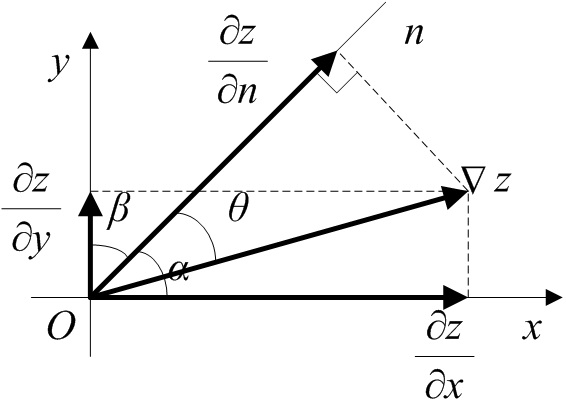
\includegraphics[height=3.5cm]{7.4.png}
\end{figure}

%============================================================
\subsection{梯度的几何意义}

几何上,梯度与等值线有垂直关系。
以二维平面的数量场为例,点$\boldsymbol{p}_0$的梯度:
\begin{itemize}
    \item 方向是等值线上该点的法向方向;
    \item 大小是$\left. \left\| \nabla z \right\| \right|_{\boldsymbol{p}_0}$。
\end{itemize}

\begin{figure}[h]
\centering
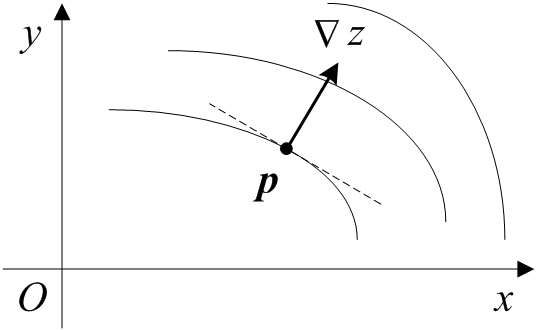
\includegraphics[height=3cm]{7.5.png}
\end{figure}

%============================================================
\subsection{梯度的物理意义}

物理上任何一个数量场,只要有变化(无变化也可以)都会有变化率,变化率可以分解到{\it xy}坐标,构成一个矢量。
所以,只有数量场才有梯度,是一个描述数量场的变化率的矢量场,其次梯度是由数量场决定的,可以认为是该数量场的性质。

%============================================================
\subsection{向量微分算子}

从纯粹的数学上,可以再进一步把“计算梯度”这一数学计算抽象出来,写成记号:
\[
\nabla :=\left( \begin{array}{c}
	\frac{\partial}{\partial x}\\
	\frac{\partial}{\partial y}\\
\end{array} \right)
\]
称为{\bf 向量微分算子},又称{\bf 哈密尔顿算子}:
\begin{itemize}
    \item 首先,它是一个算子,是纯数学上的一个计算符号,本身不承载任何物理意义;
    \item 其次是一个进行微分运算的算子;
    \item 最后是向量,表示这个微分算子是对构成其目标对象的基的微分运算,结果是一个矢量。
\end{itemize}
于是,梯度可以理解为微分算子和数量场的积,或者更简单的是“一个矢量的数乘”:
\[
\nabla z=\left( \begin{array}{c}
	\frac{\partial}{\partial x}\\
	\frac{\partial}{\partial y}\\
\end{array} \right) z=\left( \begin{array}{c}
	\frac{\partial z}{\partial x}\\
	\frac{\partial z}{\partial y}\\
\end{array} \right)
\]

~

梯度的运算法则:
\begin{align*}
&\nabla Cf=C\nabla f \\
&\nabla \left( f+g \right) =\nabla f+\nabla g \\
&\nabla \left( fg \right) =g\nabla f+f\nabla g \\
&\nabla f\left( u \right) =\frac{df}{du}\nabla u
\end{align*}






\newpage
\section{二元函数的泰勒展开}

之前在一元函数中,我们讨论了泰勒展开,这里我们进一步讨论二元函数的泰勒展开。

本节要点:
\begin{itemize}
    \item 掌握二元函数的泰勒展开;
    \item 了解黑塞矩阵。
\end{itemize}

%============================================================
\subsection{二元函数的泰勒展开}

\begin{theorem}[泰勒定理(拉格朗日型)]
若函数$f\left( x,y \right) $在$\left( x_0,y_0 \right) $的某邻域$N$内具有n+1阶连续偏导数,$\left( x_0+h,y_0+k \right) \in N$,则有:
\begin{align*}
f\left( x_0+h,y_0+k \right) =&f\left( x_0,y_0 \right) + \\
&\left( h\frac{\partial}{\partial x}+k\frac{\partial}{\partial y} \right) f\left( x_0,y_0 \right) + \\
&\frac{1}{2!}\left( h\frac{\partial}{\partial x}+k\frac{\partial}{\partial y} \right) ^2f\left( x_0,y_0 \right) + \\
&\cdots \\
&\frac{1}{n!}\left( h\frac{\partial}{\partial x}+k\frac{\partial}{\partial y} \right) ^nf\left( x_0,y_0 \right) + \\
&R_n
\end{align*}
其中:
\begin{itemize}
    \item $R_n=\frac{1}{\left( n+1 \right) !}\left( h\frac{\partial}{\partial x}+k\frac{\partial}{\partial y} \right) ^{n+1}f\left( x_0+\theta h,y_0+\theta k \right) ,\theta \in \left( 0,1 \right) $:{\bf 拉格朗日余项};
\end{itemize}
该展开称为{\bf $f\left( x,y \right) $在$\left( x_0,y_0 \right) $的$n$阶具有拉格朗日余项的泰勒公式}。
上式中的记号:
\begin{align*}
&\left( h\frac{\partial}{\partial x}+k\frac{\partial}{\partial y} \right) f\left( x_0,y_0 \right) =hf_x\left( x_0,y_0 \right) +kf_y\left( x_0,y_0 \right) \\
&\left( h\frac{\partial}{\partial x}+k\frac{\partial}{\partial y} \right) ^2f\left( x_0,y_0 \right) =h^2f_{xx}\left( x_0,y_0 \right) +2hkf_{xy}\left( x_0,y_0 \right) +k^2f_{yy}\left( x_0,y_0 \right) \\
&\left( h\frac{\partial}{\partial x}+k\frac{\partial}{\partial y} \right) ^nf\left( x_0,y_0 \right) =\sum_{i=0}^n{\left[ C_{n}^{i}h^ik^{n-i}\frac{\partial ^nf\left( x_0,y_0 \right)}{\partial x^i\partial y^{n-i}} \right]}
\end{align*}
\end{theorem}

证明略,大致是一元泰勒展开+复合函数的链式求导,详见“教材\cite{book1}”。

\begin{theorem}[泰勒定理(佩亚诺型)]
若函数$f\left( x,y \right) $在$\left( x_0,y_0 \right) $的某邻域$N$内具有n阶连续偏导数,$\left( x_0+h,y_0+k \right) \in N$,则有:
\begin{align*}
f\left( x_0+h,y_0+k \right) =&f\left( x_0,y_0 \right) + \\
&\left( h\frac{\partial}{\partial x}+k\frac{\partial}{\partial y} \right) f\left( x_0,y_0 \right) + \\
&\frac{1}{2!}\left( h\frac{\partial}{\partial x}+k\frac{\partial}{\partial y} \right) ^2f\left( x_0,y_0 \right) + \\
&\cdots \\
&\frac{1}{n!}\left( h\frac{\partial}{\partial x}+k\frac{\partial}{\partial y} \right) ^nf\left( x_0,y_0 \right) + \\
&o\left( \rho ^n \right)
\end{align*}
其中:
\begin{itemize}
    \item $\rho =\sqrt{h^2+k^2}$:{\bf 佩亚诺余项};
\end{itemize}
该展开称为{\bf $f\left( x,y \right) $在$\left( x_0,y_0 \right) $的$n$阶具有佩亚诺余项的泰勒公式}。
\end{theorem}

%============================================================
\subsection{黑塞Hessian矩阵}

当我们考虑二阶拉格朗日余项的泰勒展开:
\begin{align*}
f\left( x_0+h,y_0+k \right) =&f\left( x_0,y_0 \right) + \\
&\left( h\frac{\partial}{\partial x}+k\frac{\partial}{\partial y} \right) f\left( x_0,y_0 \right) + \\
&\frac{1}{2!}\left( h\frac{\partial}{\partial x}+k\frac{\partial}{\partial y} \right) ^2f\left( x_0,y_0 \right) + \\
&R_3
\end{align*}
其中,第二项写成向量形式:
\[
\left( h\frac{\partial}{\partial x}+k\frac{\partial}{\partial y} \right) f\left( x_0,y_0 \right) =\left( \begin{array}{c}
	h\\
	k\\
\end{array} \right) ^T\left( \begin{array}{c}
	\left. \frac{\partial f}{\partial x} \right|_{\boldsymbol{p}_0}\\
	\left. \frac{\partial f}{\partial y} \right|_{\boldsymbol{p}_0}\\
\end{array} \right) =\left( \begin{array}{c}
	h\\
	k\\
\end{array} \right) ^T\nabla f_{\boldsymbol{p}_0}
\]
第三项写成向量形式:
\begin{align*}
\left( h\frac{\partial}{\partial x}+k\frac{\partial}{\partial y} \right) ^2f\left( x_0,y_0 \right) &=h^2f_{xx}\left( \boldsymbol{p}_0 \right) +2hkf_{xy}\left( \boldsymbol{p}_0 \right) +k^2f_{yy}\left( \boldsymbol{p}_0 \right) \\
&=\left( \begin{array}{c}
	h\\
	k\\
\end{array} \right) ^T\left[ \begin{matrix}
	\left. f_{xx} \right|_{\boldsymbol{p}_0}&		\left. f_{xy} \right|_{\boldsymbol{p}_0}\\
	\left. f_{yx} \right|_{\boldsymbol{p}_0}&		\left. f_{yy} \right|_{\boldsymbol{p}_0}\\
\end{matrix} \right] \left( \begin{array}{c}
	h\\
	k\\
\end{array} \right)
\end{align*}
我们将矩阵
\[
H_f=\left[ \begin{matrix}
	f_{xx}&		f_{xy}\\
	f_{yx}&		f_{yy}\\
\end{matrix} \right]
\]
称为{\bf 函数$f\left( x,y \right) $的黑塞(Hessian)矩阵},记作$H_f$,特别地,当$f\left( x,y \right) $具有二阶连续偏导时,有$f_{xy}=f_{yx}$,于是Hessian矩阵为对称矩阵,即$H_f={H_f}^T$。

于是,二阶拉格朗日余项的泰勒展开用矩阵形式可以写成矩阵形式:
\begin{align*}
f\left( \boldsymbol{p} \right) =&f\left( \boldsymbol{p}_0 \right) + \\
&\left( \boldsymbol{p}-\boldsymbol{p}_0 \right) ^T\nabla f_{\boldsymbol{p}_0}+ \\
&\frac{1}{2!}\left( \boldsymbol{p}-\boldsymbol{p}_0 \right) ^TH_f\left( \boldsymbol{p}_0 \right) \left( \boldsymbol{p}-\boldsymbol{p}_0 \right) + \\
&R_3
\end{align*}

一元函数是标量,所以其一阶导数和二阶导数都是标量。
二元函数虽然是标量,但一阶导数(也即梯度)就是一个矢量,二阶导数就是一个$2\times 2$矩阵,这就是黑塞矩阵。
所以黑塞矩阵相当于一元函数中的二阶导数,可用于判断函数的极值。






\newpage
\section{多元函数的极值}

之前在一元函数中我们用导数讨论了极值问题,这里我们扩展到二元函数,用梯度和黑塞矩阵讨论二元函数的极值问题。

本节要点:
\begin{itemize}
    \item 掌握二元函数的极值的概念;
    \item 深刻理解二元函数极值的判断方法;
    \item 了解条件极值和拉格朗日乘数法。
\end{itemize}

%============================================================
\subsection{极值的概念}

\begin{definition}[极值]
若函数$f\left( \boldsymbol{p} \right) $在点$\boldsymbol{p}_0$的某去心邻域$N\left( \boldsymbol{\hat{p}}_0,\delta \right) $内任意一点$\boldsymbol{p}$有
\[
f\left( \boldsymbol{p} \right) >f\left( \boldsymbol{p}_0 \right) \quad \text{或} \quad f\left( \boldsymbol{p} \right) <f\left( \boldsymbol{p}_0 \right)
\]
则称$f\left( \boldsymbol{p}_0 \right) $为{\bf 函数$f\left( \boldsymbol{p} \right) $的极小值}(或{\bf 极大值}),点$\boldsymbol{p}_0$为{\bf 函数的极小值点}(或{\bf 极大值点})。
我们统称极小值和极大值为{\bf 极值},极小值点和极大值点为{\bf 极值点}。
\end{definition}

在讨论函数$f\left( \boldsymbol{p} \right) $的极值问题时,我们将$f\left( \boldsymbol{p} \right) $称为{\bf 目标函数},这类问题称为无条件极值问题。
如果加了一些限定条件如$g\left( \boldsymbol{p} \right) =0$(也可以是不等式),则称为{\bf 条件极值}。

%============================================================
\subsection{极值的判断}

类似于一元函数,二元函数的极值判断也有充分条件和必要条件。

\begin{theorem}[极值的充分条件]
若函数$f\left( \boldsymbol{p} \right) $在$\boldsymbol{p}_0$处有偏导,在$\boldsymbol{p}_0$取得极值,则:
\[
f_x\left( \boldsymbol{p}_0 \right) =f_y\left( \boldsymbol{p}_0 \right) =0
\]
用矢量写为:
\[
\nabla f\left( \boldsymbol{p}_0 \right) =\mathbf{0}
\]
符合上式的$\boldsymbol{p}_0$称为{\bf 函数的驻点}。
\end{theorem}

\begin{theorem}[极值的必要条件]
若函数$f\left( \boldsymbol{p} \right) $在$\boldsymbol{p}_0$的某邻域内有二阶连续偏导,且$f_x\left( \boldsymbol{p}_0 \right) =f_y\left( \boldsymbol{p}_0 \right) =0$,记函数$f\left( \boldsymbol{p} \right) $在$\boldsymbol{p}_0$的黑塞矩阵
\[
H_f\left( \boldsymbol{p}_0 \right) =\left. \left[ \begin{matrix}
	f_{xx}&		f_{xy}\\
	f_{yx}&		f_{yy}\\
\end{matrix} \right] \right|_{\boldsymbol{p}_0}\triangleq \left[ \begin{matrix}
	A&		B\\
	B&		C\\
\end{matrix} \right]
\]
\begin{itemize}
    \item 当$H_f\left( \boldsymbol{p}_0 \right) $为正定矩阵,即$AC>B^2,A>0$,则$f\left( \boldsymbol{p}_0 \right) $为极小值;
    \item 当$H_f\left( \boldsymbol{p}_0 \right) $为负定矩阵,即$AC>B^2,A<0$,则$f\left( \boldsymbol{p}_0 \right) $为极大值;
    \item 当$H_f\left( \boldsymbol{p}_0 \right) $为不定矩阵,即$AC<B^2$,则$f\left( \boldsymbol{p}_0 \right) $不是极值。
\end{itemize}
\end{theorem}

在二元函数中,我们用梯度判断驻点,用黑塞矩阵判断极值点。
如果要判断全部极值点,还需要判断边界点和不可导点。
和一元函数对比学习!

%============================================================
\subsection{条件极值和拉格朗日乘数法}

所谓条件极值,就是$\boldsymbol{p}$中的标量元素间有相互制约关系,这点在一元函数中是不存在的。
如计算球面上点$\boldsymbol{p}\in S$和球面外的点$\boldsymbol{q}$最近的点。
这里,$S$就是约束条件,$f\left( \boldsymbol{p} \right) =\left\| \boldsymbol{p}-\boldsymbol{q} \right\| $就是目标函数。
我们要求解的就是$f\left( \boldsymbol{p} \right) =\left\| \boldsymbol{p}-\boldsymbol{q} \right\| $的最小值。

通常带约束条件的极值判断较为复杂,拉格朗日乘数法是一个通常的解决方法,具体参见“教材\cite{book1}”。
总体思路是将约束条件带入目标函数,构造拉格朗日函数$F$,用$\nabla F=\mathbf{0}$求出驻点,最后结合边界、不可导点和问题本身的物理意义判断极值。






\newpage
\section{应用}

本节讨论多元函数微分学的两个实例。

%============================================================
\subsection{电场和电势}

设空间原点处有一电荷$q$,讨论电场和电势的关系。
三维空间某点的电势和电场表达式:
\begin{align*}
&U\left( \boldsymbol{p} \right) =\frac{q}{4\pi \varepsilon \left\| \boldsymbol{p} \right\|} \\
&\boldsymbol{E}\left( \boldsymbol{p} \right) =\frac{q}{4\pi \varepsilon \left\| \boldsymbol{p} \right\| ^2}\cdot \frac{\boldsymbol{p}}{\left\| \boldsymbol{p} \right\|}
\end{align*}
其中,$\boldsymbol{p}=\left( x\,\,y\,\,z \right) ^T$三维空间某点的坐标。

对电势求梯度,得:
\begin{align*}
&\begin{aligned}
	\because \nabla U\left( \boldsymbol{p} \right) &=\left( \begin{array}{c}
	\frac{\partial}{\partial x}\\
	\frac{\partial}{\partial y}\\
	\frac{\partial}{\partial z}\\
\end{array} \right) \frac{q}{4\pi \varepsilon \left\| \boldsymbol{p} \right\|}=\frac{q}{4\pi \varepsilon}\left( \begin{array}{c}
	\frac{\partial}{\partial x}\frac{1}{\sqrt{x^2+y^2+z^2}}\\
	\frac{\partial}{\partial y}\frac{1}{\sqrt{x^2+y^2+z^2}}\\
	\frac{\partial}{\partial z}\frac{1}{\sqrt{x^2+y^2+z^2}}\\
\end{array} \right)\\
	&=-\frac{q}{4\pi \varepsilon \left\| \boldsymbol{p} \right\| ^3}\left( \begin{array}{c}
	x\\
	y\\
	z\\
\end{array} \right) =-\frac{q}{4\pi \varepsilon \left\| \boldsymbol{p} \right\| ^3}\cdot \boldsymbol{p}\\
\end{aligned} \\
&\therefore \nabla U\left( \boldsymbol{p} \right) =-\boldsymbol{E}\left( \boldsymbol{p} \right)
\end{align*}
电荷在空间任意一点的电场为该点电势的负梯度。
即电场表示电势的变化率,且是反向的变化率。

可以想象,电势描述的是静电荷产生的静电势能,是一个数量场,就像一座山产生了重力势能。
而其变化率,或理解为这个势的“坡”,是有方向有大小的,即是一个矢量场,该矢量场就是电场。
梯度的方向是电势升高的方向为正,而电场方向是正电荷发出的方向,所以两者差了一个负号。

%============================================================
\subsection{一维波动方程}

物理上的波,指的是空间上一点的振动引起相隔的点的振动,而且这种振动以自有的速度向其他方向传播的现象。
一维空间上,假设原点有振动$y=f\left( t \right) $,该振动以速度$v$向{\it x}轴正向转播,则在$t_0$时刻,$x_0$处的质点有:
\[
y=f\left( t_0-\frac{x_0}{v} \right)
\]
可得{\it x}轴上任意一点在任意时刻的振动满足:
\[
y\left( x,t \right) =f\left( t-\frac{x}{v} \right)
\]
该振动就是{\bf 波},并会以速度$v$沿{\it x}轴方向传播。
符合该特征的函数称为{\bf 波函数}。

对波函数求偏导:
\begin{align*}
&\begin{cases}
	\frac{\partial y}{\partial x}=\frac{df}{du}\cdot \frac{\partial}{\partial x}\left( t-\frac{x}{v} \right) =-\frac{1}{v}\frac{df}{du}\\
	\frac{\partial ^2y}{\partial x^2}=-\frac{1}{v}\cdot \frac{\partial}{\partial x}\left( \frac{df}{du} \right) =-\frac{1}{v}\cdot \frac{d^2f}{du^2}\cdot \frac{\partial}{\partial x}\left( t-\frac{x}{v} \right) =\frac{1}{v^2}\frac{d^2f}{du^2}\\
\end{cases} \\
&\begin{cases}
	\frac{\partial y}{\partial t}=\frac{df}{du}\cdot \frac{\partial}{\partial t}\left( t-\frac{x}{v} \right) =\frac{df}{du}\\
	\frac{\partial ^2y}{\partial t^2}=\frac{\partial}{\partial t}\left( \frac{df}{du} \right) =\frac{d^2f}{du^2}\cdot \frac{\partial}{\partial t}\left( t-\frac{x}{v} \right) =\frac{d^2f}{du^2}\\
\end{cases}
\end{align*}
可见波函数满足如下偏微分方程:
\[
\frac{\partial ^2y}{\partial t^2}=v^2\cdot \frac{\partial ^2y}{\partial x^2}
\]
该偏微分方程称为{\bf 波动方程},同时,我们称该方程的解为{\bf 波函数}。






\newpage
\section{本章小结}

至此我们讨论完了二元函数微分学。
二元函数微分学主要讨论曲面的光滑性,我们在上一章给出了光滑曲面的第一个要求——不断,本章讨论了第二个要求——不折。
我们定义了偏导数、方向导数,并给出了二元函数微分学的一个核心概念——全微分。
如果曲面在一点满足全微分要求,几何上就代表在该点有切平面。
最后我们讨论了梯度,我们将一个曲面的变化率按照自变量坐标系分解得到一个矢量形式的变化率。
我们还举例了微分的实际用处——估值。

学习本章特别要和一元函数微分学中的定义对比。
同样是“以直代曲”,一元函数微分学中较为简单,而由于二元函数中$z$的变化量不光取决于$x,y$各自变化,还有它们联合产生的效果。

下面的积分章节,我们要讨论光滑在“累积”方面有哪些特征,可以帮助我们解决什么问题。






\newpage
\section{习题}

\begin{exercise}
求下列函数的偏导数:
\begin{enumerate}
    \item $z=e^{xy}\cos \left( x+2y \right) $
    \item $z=\mathrm{arc}\tan \sqrt{x^y}$
    \item $u=\left( \frac{x}{y} \right) ^z$
\end{enumerate}
\end{exercise}

解:

1.
\begin{align*}
&\frac{\partial z}{\partial x}=ye^{xy}\cos \left( x+2y \right) -e^{xy}\sin \left( x+2y \right) \\
&\frac{\partial z}{\partial y}=xe^{xy}\cos \left( x+2y \right) -2e^{xy}\sin \left( x+2y \right)
\end{align*}

2.
\begin{align*}
&\frac{\partial z}{\partial x}=\frac{1}{1+x^y}\cdot \frac{1}{2\sqrt{x^y}}\cdot yx^{y-1} \\
&\frac{\partial z}{\partial y}=\frac{1}{1+x^y}\cdot \frac{1}{2\sqrt{x^y}}\cdot x^y\ln x
\end{align*}

3.
\begin{align*}
&\frac{\partial u}{\partial x}=z\left( \frac{x}{y} \right) ^{z-1}\cdot \frac{1}{y} \\
&\frac{\partial u}{\partial y}=z\left( \frac{x}{y} \right) ^{z-1}\cdot \left( -\frac{x}{y^2} \right) \\
&\frac{\partial u}{\partial z}=\left( \frac{x}{y} \right) ^z\cdot \ln \left( \frac{x}{y} \right)
\end{align*}

~

\begin{exercise}
若函数$z=\frac{\ln \left( xy \right)}{y}$,求全微分。
\end{exercise}

解:
\begin{align*}
dz&=\frac{\partial z}{\partial x}dx+\frac{\partial z}{\partial y}dy=\frac{1}{y}\frac{1}{xy}y\cdot dx+\frac{\frac{1}{xy}xy-\ln \left( xy \right)}{y^2}\cdot dy \\
&=\frac{1}{xy}\cdot dx+\frac{1-\ln \left( xy \right)}{y^2}\cdot dy
\end{align*}

~

\begin{exercise}
计算下列各式的近似值:
\begin{enumerate}
    \item $\sqrt{1.02^3+1.97^3}$
    \item $0.97^{1.05}$
\end{enumerate}
\end{exercise}

解:

1.
构造$z=f\left( \boldsymbol{p} \right) =\sqrt{x^3+y^3},\boldsymbol{p}_0=\left( 1,2 \right) ,dx=0.02,dy=-0.03$,于是:
\begin{align*}
\sqrt{1.02^3+1.97^3}&\approx z\left( 1,2 \right) +\frac{\partial z}{\partial x}dx+\frac{\partial z}{\partial y}dy \\
&=3+\frac{3x^2}{2\sqrt{x^3+y^3}}dx+\frac{3y^2}{2\sqrt{x^3+y^3}}dy=2.95 \\
\sqrt{1.02^3+1.97^3}&=2.95069
\end{align*}

2.
构造$z=f\left( \boldsymbol{p} \right) =x^y,\boldsymbol{p}_0=\left( 1,1 \right) ,dx=-0.03,dy=0.05$,于是:
\begin{align*}
0.97^{1.05}&\approx z\left( 1,1 \right) +\frac{\partial z}{\partial x}dx+\frac{\partial z}{\partial y}dy \\
&=1+yx^{y-1}\cdot dx+x^y\ln x\cdot dy=0.97 \\
0.97^{1.05}&=0.968524
\end{align*}

~

\begin{exercise}
有一半径5cm,高20cm的金属圆柱体100个,现要在其表面镀一层厚度为0.05cm的镍,估计需要多少镍,已知镍的比重8.8g/cm3。
\end{exercise}

解:

总体思路是估算100个圆柱体的体积增量。
对圆柱体体积计算公式进行全微分:
\begin{align*}
&V\left( r,h \right) =\pi r^2h \\
&dV\left( r,h \right) =2\pi rh\cdot dr+\pi r^2\cdot dh
\end{align*}
于是,镍需要:
\begin{align*}
m&=100\cdot dV\cdot \rho =100\cdot \left( 2\pi rh\cdot dr+\pi r^2\cdot dh \right) \cdot \rho \\
&=100\cdot \left( 2\pi \cdot 5\cdot 20\cdot 0.05+\pi \cdot 5^2\cdot 0.10 \right) \cdot 8.8=34557.5\mathrm{g}
\end{align*}

~

\begin{exercise}
设有一无盖圆柱形容器,壁和底的厚度均为0.1cm,内高20cm,半径4cm,求外壳体积的近似值。
\end{exercise}

解:

总体思路依然是估算圆柱体体积的增量。
\begin{align*}
&V\left( r,h \right) =\pi r^2h \\
&dV\left( r,h \right) =2\pi rh\cdot dr+\pi r^2\cdot dh
\end{align*}

于是:
\begin{align*}
dV&=2\pi rh\cdot dr+\pi r^2\cdot dh \\
&=2\pi \cdot 4\cdot 20\cdot 0.1+\pi \cdot 4^2\cdot 0.1=55.292\mathrm{cm}^3
\end{align*}










\chapter{多重积分}

多元函数积分学,根据多维空间为标量还是向量分为:
\begin{itemize}
    \item 多元数量值函数积分;
    \item 多元向量值函数积分。
\end{itemize}
本章简称“数量积分”和“向量积分”。
之前的一元函数积分学本章简称“一元积分”。

数量积分的物理应用对应诸如三维体质量、薄型平板电荷总量等。
数量积分是一元积分的多维扩展,被积函数从一元扩展到多元,微元也从一元扩展到多元。
通常来讲,被积函数是给出的,如三维体的体密度,不需要特别处理,关键要解决多维空间里微元的表达,解决了这个表达式,就能很容易化为一元积分。

本章介绍最基础的多重积分,多重积分是后续曲线积分和曲线积分的基础。

本章要点:
\begin{itemize}
    \item 多重积分的概念。
    \item 二重积分和三重积分的计算。
\end{itemize}

~

\newpage
\section{多元数量值函数积分的概念}

本节讨论多元数量积分的概念、性质、分类。

本节要点:
\begin{itemize}
    \item 掌握数量积分的概念;
    \item 掌握数量积分的性质。
\end{itemize}

%============================================================
\subsection{多元数量值函数积分的概念}

\begin{definition}[数量积分]
假设$\varOmega $为一可度量的有界的封闭几何体,函数$f$是定义在$\varOmega $上的一个有界的数量值函数,将$\varOmega $任意划分为$n$个小部分,并用$\Delta \varOmega _i$表示每一个小部分的度量,在每一个小部分上任取一点$M_i$,作乘积后再作和式:
\[
\sum_{i=1}^n{\left[ f\left( M_i \right) \cdot \Delta \varOmega _i \right]}
\]
记$\lambda =\max \left\{ diameter \ of \ \Delta \varOmega _i \right\} $,如果不论对$\varOmega $如何划分,也不论点$M_i$在$\varOmega $中如何选取,若当$\lambda \rightarrow 0$时上述和式有极限且相等,则称{\bf 函数$f$在$\varOmega $上可积},此极限值称为{\bf 多元数量值函数$f$在几何体$\varOmega $上的积分},记作$\int_{\varOmega}{f\left( M \right) d\varOmega}$,即:
\[
\int\limits_{\varOmega}{f\left( M \right) d\varOmega}:=\underset{\lambda \rightarrow 0}{\lim}\sum_{i=1}^n{\left[ f\left( M_i \right) \cdot \Delta \varOmega _i \right]}
\]
其中:
\begin{itemize}
    \item $\varOmega $:{\bf 积分区域},可以是二维、三维、甚至$n$维,并没有规定维度;
    \item $f$:{\bf 被积函数},是几何体$\varOmega $相应的维度的数量值函数,如果$\varOmega $是二维,则$f$是二元函数,如果$\varOmega $是三维,则$f$是三元函数。
\end{itemize}
\end{definition}

数学上,数量积分依旧是“加权和”的概念,$d\varOmega $对应加权$f\left( M \right) $后,在$\varOmega $范围内的和。

\begin{theorem}[存在性定理]
如果函数$f$在有界闭几何体$\varOmega $上是连续的,则$f$在$\varOmega $上必可积。
\end{theorem}

%============================================================
\subsection{多元数量值函数积分的性质和定理}

线性性:
\[
\int\limits_{\varOmega}{\left[ af\left( M \right) +bg\left( M \right) \right] d\varOmega}=a\int\limits_{\varOmega}{f\left( M \right) d\varOmega}+b\int\limits_{\varOmega}{g\left( M \right) d\varOmega}
\]

区域可加性:
\[
\int\limits_{\varOmega}{f\left( M \right) d\varOmega}=\int\limits_{\varOmega _1}{f\left( M \right) d\varOmega}+\int\limits_{\varOmega _2}{f\left( M \right) d\varOmega}
\]

不等式性质:
\[
f\left( M \right) \leqslant g\left( M \right) \quad \Rightarrow \quad \int\limits_{\varOmega}{f\left( M \right) d\varOmega}\leqslant \int\limits_{\varOmega}{g\left( M \right) d\varOmega}
\]

~

\begin{theorem}[估值定理]
设$m,M$分别是$f$在闭几何体$\varOmega $上的最小值和最大值,则:
\[
m\int\limits_{\varOmega}{d\varOmega}\leqslant \int\limits_{\varOmega}{f\left( M \right) d\varOmega}\leqslant M\int\limits_{\varOmega}{d\varOmega}
\]
\end{theorem}

\begin{theorem}[积分中值定理]
设$f$在闭几何体$\varOmega $上连续,则存在$M_0\in \varOmega $,有:
\[
\int\limits_{\varOmega}{f\left( M \right) d\varOmega}=f\left( M_0 \right) \int\limits_{\varOmega}{d\varOmega}
\]
\end{theorem}

\begin{theorem}[对称性定理]
当积分域$\varOmega $关于$x$对称时,
\begin{itemize}
    \item 若$f$关于$x=0$为奇函数,则$\int_{\varOmega}{f\left( M \right) d\varOmega}=0$;
    \item 若$f$关于$x=0$为偶函数,则$\int_{\varOmega}{f\left( M \right) d\varOmega}=2\int_{\varOmega '}{f\left( M \right) d\varOmega}$,其中$\varOmega '$为$\varOmega $ 位于$x<0$部分。
\end{itemize}
\end{theorem}






\newpage
\section{二重积分}

本节讨论二重积分的定义、意义和计算方法。

本节要点:
\begin{itemize}
    \item 掌握二重积分的定义;
    \item 了解二重积分的数学意义、物理意义和几何意义;
    \item 掌握二重积分在直角坐标下的计算方法;
    \item 了解二重积分在极坐标下的计算方法。
\end{itemize}

%============================================================
\subsection{二重积分的概念}

\begin{definition}[二重积分]
若$f\left( \boldsymbol{p} \right) $是定义在平面区域$D$上的二元数量值函数,则将{\bf $f\left( \boldsymbol{p} \right) $在$D$上的积分为二重积分}写成:
\begin{align*}
&\iint\limits_D{f\left( \boldsymbol{p} \right) d\sigma} \\
&D=\left\{ \left( x,y \right) \middle| x_1\leqslant x\leqslant x_2,y_1\left( x \right) \leqslant y\leqslant y_2\left( x \right) \right\}
\end{align*}
其中:
\begin{itemize}
    \item $f\left( \boldsymbol{p} \right) $:{\bf 被积函数};
    \item $d\sigma$:{\bf 积分微元};
    \item $D$:{\bf 积分区域}。
\end{itemize}
\end{definition}

这里需要注意一个地方。
$f\left( \boldsymbol{p} \right) $是一个二元数量值函数,也可以写成$z=z\left( x,y \right) $,$z$被$x,y$约束,$x,y$之间没有约束关系,反应几何上的一个曲面。
但是作为定积分,{\it xOy}平面上还是有一个积分区域的,它被一组曲线(或直线)包围,所以$y_1\left( x \right) \leqslant y\leqslant y_2\left( x \right) $描述的是这个积分区域,而不是$x,y$的约束关系。

%============================================================
\subsection{二重积分的几何意义和物理意义}

对比一元积分,二重积分在数学上是对一个指定平面的“加权和”。
\begin{align*}
&\int_a^b{f\left( x \right) dx} \quad x\in \left[ a,b \right] \\
&\iint\limits_D{f\left( \boldsymbol{p} \right) d\sigma} \quad D=\left\{ \left( x,y \right) \middle| x_1\leqslant x\leqslant x_2,y_1\left( x \right) \leqslant y\leqslant y_2\left( x \right) \right\}
\end{align*}
几何上,这个“权”可以由{\it z}轴表示,则二重积分的几何意义可以理解为以$D$为底、$f\left( \boldsymbol{p} \right) $为曲顶的曲顶柱体的体积。

物理上,如果这个“权”是密度,则二重积分表示这个指定平面的总质量,如果这个“权”是电荷密度,则二重积分表示这个指定平面的总电荷量。

\begin{figure}[h]
\centering
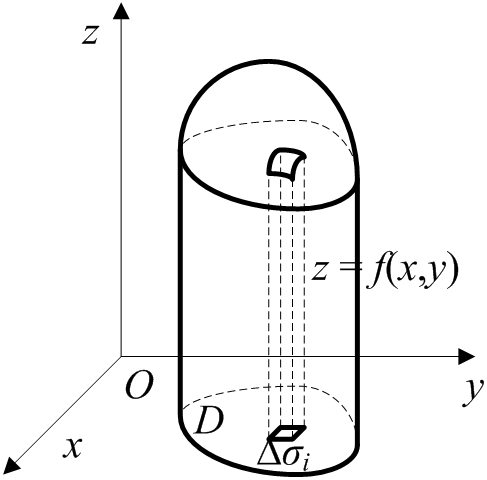
\includegraphics[height=4cm]{8.1.png}
\end{figure}

%============================================================
\subsection{二重积分的直角坐标计算}

总体来讲,二重积分的计算归根结底要化为一元积分,就是要将微元和被积函数都一元化。
在直角坐标下,面积微元可以表示为$d\sigma =dxdy$,于是:
\begin{align*}
&\iint\limits_D{f\left( \boldsymbol{p} \right) d\sigma}=\iint\limits_D{f\left( x,y \right) dxdy} \\
&D=\left\{ \left( x,y \right) \middle| x_1\leqslant x\leqslant x_2,y_1\left( x \right) \leqslant y\leqslant y_2\left( x \right) \right\}
\end{align*}
$D$可以理解为由两条直线$x=x_1,x=x_2$和两条曲线$y=y_1\left( x \right) ,y=y_2\left( x \right) $围成。
其次,将被积函数一元化。
曲顶柱体的体积的求解可以通过“切片”处理,先处理“一片”,再将“片”累加起来。

计算步骤:
\begin{enumerate}
    \item 计算$x_0$时的薄片的面积,即将$x_0$看成常数,求$y$从$y_1\left( x_0 \right) $到$y_2\left( x_0 \right) $的定积分,此时$f\left( x,y \right) $变为一元函数,薄片面积$S\left( x \right) $是$x$的函数
    \[
    S\left( x_0 \right) =\int_{y_1\left( x_0 \right)}^{y_2\left( x_0 \right)}{f\left( x_0,y \right) dy}
    \]
    \item 将这些薄片累积,即为该二重积分的结果
    \[
    \iint\limits_D{f\left( x,y \right) dxdy}=\int_{x_1}^{x_2}{S\left( x \right) dx}=\int_{x_1}^{x_2}{\left[ \int_{y_1\left( x \right)}^{y_2\left( x \right)}{f\left( x,y \right) dy} \right] dx}
    \]
\end{enumerate}

上式即为在直角坐标下二重积分$\iint_D{f\left( x,y \right)}$在区域$D$上的计算公式,常写作:
\begin{align*}
&\iint\limits_D{f\left( x,y \right) d\sigma}=\int_{x_1}^{x_2}{dx\int_{y_1\left( x \right)}^{y_2\left( x \right)}{f\left( x,y \right) dy}} \\
&D=\left\{ \left( x,y \right) \middle| x_1\leqslant x\leqslant x_2,y_1\left( x \right) \leqslant y\leqslant y_2\left( x \right) \right\}
\end{align*}
类似地,若积分区域$D$由两条直线$y=y_1,y=y_2$和两条曲线$x=x_1\left( y \right) ,x=x_2\left( y \right) $围成,则有:
\begin{align*}
&\iint\limits_D{f\left( x,y \right) d\sigma}=\int_{y_1}^{y_2}{dy\int_{x_1\left( y \right)}^{x_2\left( y \right)}{f\left( x,y \right) dx}} \\
&D=\left\{ \left( x,y \right) \middle| x_1\left( y \right) \leqslant x\leqslant x_2\left( y \right) ,y_1\leqslant y\leqslant y_2 \right\}
\end{align*}
最后要注意,如果积分区域$D$为凸区域,则二重积分结果和积分次序无关。

~

\begin{example}
计算$\iint_D{xyd\sigma}$,其中$D$由$y=x$和$y=x^2$围成。
\end{example}

解:

易得,围成的区域可以表示为$D=\left\{ \left( x,y \right) \middle| 0\leqslant x\leqslant 1,x^2\leqslant y\leqslant x \right\} $。
\begin{figure}[h]
\centering
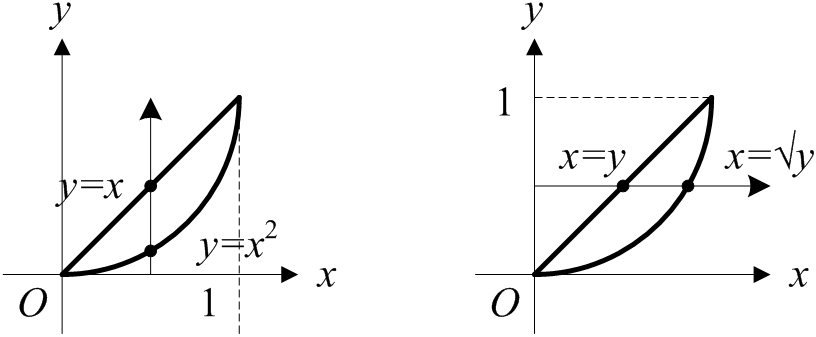
\includegraphics[height=3cm]{8.2.png}
\end{figure}
\begin{align*}
\iint\limits_D{f\left( x,y \right) d\sigma}&=\int_0^1{dx\int_{x^2}^x{xydy}}=\int_0^1{dx\left[ \left. \frac{1}{2}xy^2 \right|_{x^2}^{x} \right]} \\
&=\int_0^1{\left( \frac{1}{2}x^3-\frac{1}{2}x^5 \right) dx}=\frac{1}{24}
\end{align*}
也可以看成$D=\left\{ \left( x,y \right) \middle| y\leqslant x\leqslant \sqrt{y},0\leqslant y\leqslant 1 \right\} $:
\begin{align*}
\iint\limits_D{f\left( x,y \right) d\sigma}&=\int_0^1{dy\int_y^{\sqrt{y}}{xydx}}=\int_0^1{dy\left[ \left. \frac{1}{2}x^2y \right|_{y}^{\sqrt{y}} \right]} =\frac{1}{24}
\end{align*}

~

\begin{example}
求由柱面$x^2+y^2=R^2$和$x^2+z^2=R^2$所围成的立体(称为牟合立方)的体积。
\begin{figure}[ht]
\centering
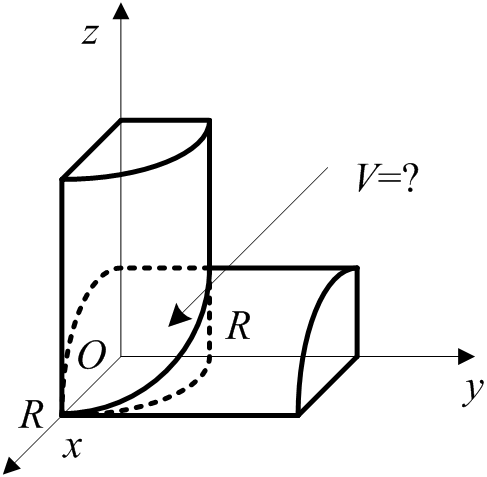
\includegraphics[height=3.5cm]{8.3.png}
\end{figure}
\end{example}

解:

以计算第一卦限为例。
该题可以理解成求一个均匀体的体积,可以用二重积分计算。
横的柱面的{\it z}轴值可以理解为高,纵的柱面在{\it xOy}平面的区域可以理解为积分区域,得到被积函数和积分区域:
\begin{align*}
&z\left( x,y \right) =\sqrt{R^2-x^2} \\
&D=\left\{ \left( x,y \right) \middle| 1\leqslant x\leqslant R,0\leqslant y\leqslant \sqrt{R^2-x^2} \right\}
\end{align*}
得到第一卦限部分的体积:
\begin{align*}
V&=\iint\limits_D{z\left( x,y \right) d\sigma}=\iint\limits_D{\sqrt{R^2-x^2}d\sigma} \\
&=\int_0^R{dx\int_0^{\sqrt{R^2-x^2}}{\sqrt{R^2-x^2}dy}}=\int_0^R{\left( R^2-x^2 \right) dx}=\frac{2}{3}R^2
\end{align*}

%============================================================
\subsection{二重积分的极坐标计算}

极坐标$\left( r,\theta \right) $的计算,在数学上和直角坐标一样:
\begin{align*}
&\iint\limits_D{f\left( r,\theta \right) d\sigma} \\
&D=\left\{ \left( r,\theta \right) \middle| \theta _1\leqslant \theta \leqslant \theta _2,r_1\left( \theta \right) \leqslant r\leqslant r_2\left( \theta \right) \right\}
\end{align*}
求解过程和直角坐标一样。
但如果方程以直角坐标的形式的给出,需要转换到极坐标。
这里,需要对变量进行变换以得到新的被积函数,还需要对$d\sigma $进行计算得到极坐标下的表达式。

坐标变换:
\[
\begin{cases}
	x=r\cos \theta\\
	y=r\sin \theta\\
\end{cases}
\]
微元$d\sigma $计算:
\begin{align*}
&\because \Delta \sigma =\frac{1}{2}\left( r+\Delta r \right) ^2\Delta \theta -\frac{1}{2}r^2\Delta \theta =r\Delta r\Delta \theta +\frac{1}{2}\Delta r^2\Delta \theta \\
&\therefore d\sigma =r\cdot drd\theta
\end{align*}
所以,直角坐标和极坐标的转换公式为:
\[
\iint\limits_D{f\left( x,y \right) dxdy}=\iint\limits_D{\left[ f\left( r\cos \theta ,r\sin \theta \right) \cdot r \right] drd\theta}
\]

二重积分,无论在直角坐标下计算,还是极坐标下计算,计算过程是一样的——“切片+累加”。
只是如果被积函数含有“弧状”(如$x^2+y^2$),极坐标下求解不定积分就会方便。

~

\begin{example}
计算以半径$R$的圆形为底,$H$为高的圆柱体体积。
\end{example}

解:

分析题干,相当于计算一个二重积分,被积函数恒为$H$,积分区域为一个圆,可假设该圆在圆心。
根据对称性,只要计算第一象限即可。
\[
V=4\iint\limits_D{Hd\sigma}=4\iint\limits_D{Hdxdy}
\]
直角坐标下,这个不定积分难解,换到极坐标就好解了。
将得到的式子转成极坐标求解:
\begin{align*}
V&=4\iint\limits_D{Hdxdy}=4\iint\limits_D{Hrdrd\theta}=4H\int_0^R{dr\int_0^{\pi /2}{rd\theta}} \\
&=4H\int_0^R{\frac{1}{2}\pi rdr}=\pi R^2H
\end{align*}
注意,这里虽然积分区域$D$没变,但是在极坐标下的表达式变了:
\begin{align*}
&D\left\{ \left( x,y \right) \middle| 0\leqslant x\leqslant R,0\leqslant y\leqslant \sqrt{R^2-x^2} \right\} \\
&\downarrow \\
&D\left\{ \left( r,\theta \right) \middle| 0\leqslant \theta \leqslant \frac{\pi}{2},0\leqslant r\leqslant R \right\}
\end{align*}






\newpage
\section{三重积分}

本节讨论三重积分的定义、意义和计算方法。

本节要点:
\begin{itemize}
    \item 掌握三重积分的定义;
    \item 了解三重积分的数学意义和物理意义;
    \item 掌握三重积分在直角坐标下的计算方法。
\end{itemize}

%============================================================
\subsection{三重积分的概念}

\begin{definition}[三重积分]
若$f\left( \boldsymbol{p} \right) $是定义在空间区域$V$上的三元数量值函数,则将{\bf $f\left( \boldsymbol{p} \right) $在$V$上的积分为三重积分}写成:
\begin{align*}
&\iiint\limits_V{f\left( \boldsymbol{p} \right) dv} \\
&V=\left\{ \left( x,y,z \right) \middle| x\in \left[ x_1,x_2 \right] ,y\in \left[ y_1\left( x \right) ,y_2\left( x \right) \right] ,z\in \left[ z_1\left( x,y \right) ,z_2\left( x,y \right) \right] \right\}
\end{align*}
其中:
\begin{itemize}
    \item $f\left( \boldsymbol{p} \right) $:{\bf 被积函数};
    \item $d\sigma$:{\bf 积分微元};
    \item $V$:{\bf 积分区域}。
\end{itemize}
\end{definition}

%============================================================
\subsection{三重积分的几何意义和物理意义}

对比一元积分和二重积分,三重积分在几何上是对一个指定三维空间的“加权和”。
\begin{align*}
&\int_a^b{f\left( x \right) dx} \quad x\in \left[ a,b \right] \\
&\iint\limits_D{f\left( \boldsymbol{p} \right) d\sigma} \quad D=\left\{ \left( x,y \right) \middle| x\in \left[ x_1,x_2 \right] ,y\in \left[ y_1,y_2 \right] \right\} \\
&\iiint\limits_V{f\left( \boldsymbol{p} \right) dv} \quad V=\left\{ \left( x,y,z \right) \middle| x\in \left[ x_1,x_2 \right] ,y\in \left[ y_1,y_2 \right] ,z\in \left[ z_1,z_2 \right] \right\}
\end{align*}

物理上,如果这个“权”是密度,则三重积分表示这个指定三维物体的总质量。
如果这个“权”是电荷密度,则三重积分表示这个指定三维物体的总电荷量。

%============================================================
\subsection{三重积分的直角坐标计算}

三重积分的计算思路和二重一样,将微元和被积函数都一元化。
被积函数一元化的方式依然采用“切片”方法。
在直角坐标下,体积微元可以表示为$dv=dxdydz$,于是:
\begin{align*}
&\iiint\limits_V{f\left( \boldsymbol{p} \right) dv}=\iiint\limits_V{f\left( x,y,z \right) dxdydz} \\
&V=\left\{ \left( x,y,z \right) \middle| x\in \left[ x_1,x_2 \right] ,y\in \left[ y_1\left( x \right) ,y_2\left( x \right) \right] ,z\in \left[ z_1\left( x,y \right) ,z_2\left( x,y \right) \right] \right\}
\end{align*}
三重积分的求解和二重积分类似,只是多了一个“切片”。

计算步骤:
\begin{enumerate}
    \item 先将$x_0,y_0$看成常数,对$z$求从$z_1\left( x_0,y_0 \right) $到$z_2\left( x_0,y_0 \right) $的定积分
    \[
    S\left( x_0,y_0 \right) =\int_{z_1\left( x_0,y_0 \right)}^{z_2\left( x_0,y_0 \right)}{f\left( x_0,y_0,z \right) dz}
    \]
    \item 再将该函数在$D$作二重积分
    \[
    \iint\limits_D{S\left( x,y \right) d\sigma}=\iint\limits_D{\left[ \int_{z_1\left( x,y \right)}^{z_2\left( x,y \right)}{f\left( x,y,z \right) dz} \right] d\sigma}
    \]
    或常写作:
    \[
    \iiint\limits_V{f\left( x,y,z \right) dv}=\iint\limits_D{dxdy\int_{z_1\left( x,y \right)}^{z_2\left( x,y \right)}{f\left( x,y,z \right) dz}}
    \]
\end{enumerate}

通过以上方法,化为了二重积分,后续过程略。
同样,三重积分可以在柱坐标和球坐标下计算。






\newpage
\section{多重积分的应用}

本节以物体中心为例说明多重积分的应用。

%============================================================
\subsection{物体重心}

重心即为对参考点的等效力矩的坐标。
取坐标原点为参考点。
假设三维体$\varOmega $有不均匀体密度$\rho \left( \boldsymbol{p} \right) $,则总重量:
\[
m=\iiint\limits_{\varOmega}{\rho \left( \boldsymbol{p} \right) d\sigma}
\]

首先考察三维体对{\it yOz}平面的总力矩:
\[
M_{yOz}=\iiint\limits_{\varOmega}{x\rho \left( \boldsymbol{p} \right) d\sigma}
\]
可得对于{\it yOz}平面的等效力矩的坐标:
\[
X=\frac{M_{yOz}}{m}=\frac{\iiint\limits_{\varOmega}{x\rho \left( \boldsymbol{p} \right) d\sigma}}{\iiint\limits_{\varOmega}{\rho \left( \boldsymbol{p} \right) d\sigma}}
\]

同理可得对于其他平面的等效力矩的坐标,略。






\newpage
\section{本章小结}

多重积分在数学上是一个$n$元函数在$n$维空间的积分。
\begin{figure}[h]
\centering
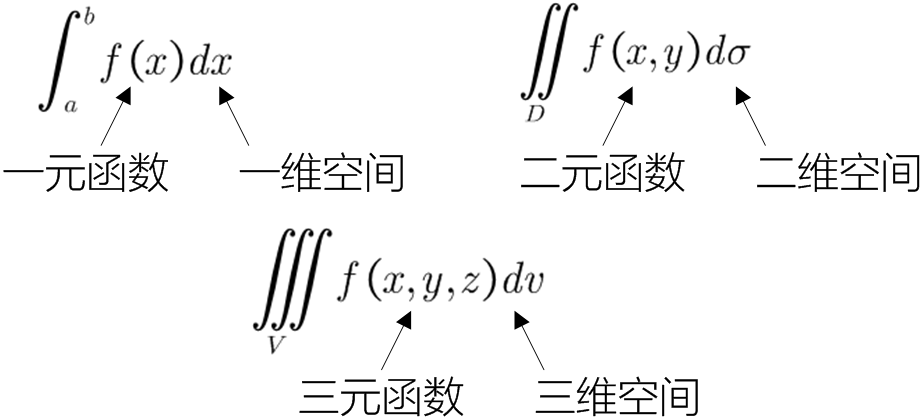
\includegraphics[height=3.5cm]{8.4.png}
\end{figure}

多重积分的物理意义非常简单明了,即已知$n$维体的体密度,求解该$n$维体的总重量。
如下表示线重量、面重量、体重量:
\begin{align*}
&W=\int_a^b{\rho \left( x \right) dx} \\
&W=\iint\limits_D{\rho \left( \boldsymbol{p} \right) d\sigma} \\
&W=\iiint\limits_V{\rho \left( \boldsymbol{p} \right) dv}
\end{align*}

多重积分的计算,总体步骤也非常明了:
\begin{enumerate}
    \item 固定$n-1$维,剩下一维变量进行积分,相当于求解一个一元函数积分,只是积分上下限是一个包含其余$n-1$维变量的表达式;
    \item 继续反复上面的步骤,直到剩下一维;
    \item 求解该一元积分。
\end{enumerate}
被积函数(即权重函数、或称密度函数)是给定的。
难点在于确定各个维度的积分上下限,即对于给定的积分区域求解各个维度的相互关系。










\chapter{曲线积分}

本章讨论第一类曲线积分和第二类曲线积分。

“第一类曲线积分”是数量值函数对曲线的积分,表示数量值对于一个曲线路径的累积量,和重积分的区别在于积分区域,除此之外没有任何区别。
“第二类曲线积分”是向量值函数对曲线的积分,是向量值在某个方向上的,具体说是在某点处的曲线方向的投影对曲线路径的累积量,与第一类曲线积分相比,多了一个“投影”步骤,表达式上是两个矢量的内积。

本章要点:
\begin{itemize}
    \item 第一类曲线积分。
    \item 第二类曲线积分。
\end{itemize}

~

\newpage
\section{第一类曲线积分}

本节讨论第一类曲线积分。
所谓“第一类曲线积分”是数量值函数对曲线的积分。

本节要点:
\begin{itemize}
    \item 掌握第一类曲线积分的概念;
    \item 掌握第一类曲线积分的计算,重点掌握弧微分的计算。
\end{itemize}

%============================================================
\subsection{第一类曲线积分的概念}

\begin{definition}[第一类曲线积分]
若三维空间中有曲线$L$,$f\left( \boldsymbol{p} \right) ,\boldsymbol{p}\in \mathbb{R} ^3$为定义在该空间上的三元数量值函数,若下式极限存在,则称极限值为{\bf $f\left( \boldsymbol{p} \right) $在$L$上积分称为第一类曲线积分},记为$\int_L{f\left( \boldsymbol{p} \right) dl}$,即:
\[
\int\limits_L{f\left( \boldsymbol{p} \right) dl}:=\underset{\lambda \rightarrow 0}{\lim}\sum_{i=1}^n{\left[ f\left( \xi _i,\eta _i,\zeta _i \right) \cdot \Delta l_i \right]}
\]
其中:
\begin{itemize}
    \item $f\left( \boldsymbol{p} \right) $:{\bf 被积函数};
    \item $dl$:{\bf 弧微分};
    \item $L$:{\bf 积分曲线}。
\end{itemize}
\end{definition}

\begin{tcolorbox}
实际定义参考“教材\cite{book1}”,这里是一个简写,总体来讲就是将曲线分段,每段上取一个值和这一小段弧长乘积$f\left( \xi _i,\eta _i,\zeta _i \right) \cdot \Delta l_i$,如果和式有极限,则称为$f\left( \boldsymbol{p} \right) $在$L$上有第一类曲线积分。
大致思路和一元函数积分一样。
\end{tcolorbox}

第一类曲线积分的性质:
\begin{itemize}
    \item 线性性:
    \[
    \int\limits_L{\left( af+bg \right) dl}=a\int\limits_L{fdl}+b\int\limits_L{gdl}
    \]
    \item 区域可加性:
    \[
    \int\limits_L{fdl}=\int\limits_{L_1}{fdl}+\int\limits_{L_2}{fdl}
    \]
\end{itemize}

同样,可定义$n$维空间上的数量值函数$f\left( \boldsymbol{p} \right) ,\boldsymbol{p}\in \mathbb{R} ^n$对空间内曲线$L$上积分为$f\left( \boldsymbol{p} \right) $在$n$维空间曲线$L$上的第一类曲线积分,记为$\int_L{f\left( \boldsymbol{p} \right) dl}$。

%============================================================
\subsection{第一类曲线积分的计算}

\begin{theorem}[第一类曲线积分的计算公式]
设三维空间上有曲线$L$,则曲线可以写为:
\[
L:\begin{cases}
	x=x\left( t \right)\\
	y=y\left( t \right)\\
	z=z\left( t \right)\\
\end{cases}
\]
弧微分的表达式:
\begin{align*}
dl&=\sqrt{\left( dx \right) ^2+\left( dy \right) ^2+\left( dz \right) ^2}=\sqrt{\left( x'dt \right) ^2+\left( y'dt \right) ^2+\left( z'dt \right) ^2} \\
&=\sqrt{\left( x' \right) ^2+\left( y' \right) ^2+\left( z' \right) ^2}\cdot dt
\end{align*}
若$f\left( \boldsymbol{p} \right) $在曲线$L$的$\left[ t_1,t_2 \right] $上连续,其中$x\left( t \right) ,y\left( t \right) ,z\left( t \right) $在$\left[ t_1,t_2 \right] $上具有一阶连续导数,则第一类曲线积分可计算为:
\[
\int\limits_L{f\left( \boldsymbol{p} \right) \cdot dl}=\int\limits_L{f\left( x,y,z \right) \cdot \sqrt{\left( x' \right) ^2+\left( y' \right) ^2+\left( z' \right) ^2}\cdot dt}
\]
\end{theorem}






\newpage
\section{第二类曲线积分}

本节讨论第二类曲线积分。
所谓“第二类曲线积分”是向量值函数对曲线的积分。

本节要点:
\begin{itemize}
    \item 掌握第二类曲线积分的概念;
    \item 掌握第二类曲线积分的计算,重点掌握积分表达式的内积计算。
\end{itemize}

%============================================================
\subsection{第二类曲线积分的概念}

\begin{definition}[第二类曲线积分]
若三维空间中有曲线$L$,$\mathbf{n}\left( \boldsymbol{p} \right) $为曲线上任一点处的单位切向量,$\boldsymbol{f}\left( \boldsymbol{p} \right) $为定义在该空间上的三元向量值函数,若内积$\boldsymbol{f}\left( \boldsymbol{p} \right) ^T\mathbf{n}\left( \boldsymbol{p} \right) $在$L$上的第一类曲线积分存在,则称此积分值为{\bf $\boldsymbol{f}\left( \boldsymbol{p} \right) $在$L$上的第二类曲线积分},记为$\int_L{\left[ \boldsymbol{f}\left( \boldsymbol{p} \right) ^T\mathbf{n}\left( \boldsymbol{p} \right) \right] \cdot dl}$,由于$\mathbf{n}\left( \boldsymbol{p} \right) dl=\boldsymbol{dl}$为弧微分在{\it xyz}坐标的投影向量,所以也可以写为$\int_L{\boldsymbol{f}\left( \boldsymbol{p} \right) ^T\boldsymbol{dl}}$,即:
\begin{align*}
&\int\limits_L{\left[ \boldsymbol{f}\left( \boldsymbol{p} \right) ^T\mathbf{n}\left( \boldsymbol{p} \right) \right] \cdot dl}=\int\limits_L{\boldsymbol{f}\left( \boldsymbol{p} \right) ^T\boldsymbol{dl}} \\
&:=\underset{\lambda \rightarrow 0}{\lim}\sum_{i=1}^n{\left[ \boldsymbol{f}\left( \xi _i,\eta _i,\zeta _i \right) ^T\mathbf{n}\left( \xi _i,\eta _i,\zeta _i \right) \cdot \Delta l_i \right]}
\end{align*}
其中:
\begin{itemize}
    \item $\boldsymbol{f}\left( \boldsymbol{p} \right) $:{\bf 被积函数};
    \item $\mathbf{n}\left( \boldsymbol{p} \right) $:曲线上任一点处的{\bf 单位切向量},也即切线的方向余弦;
    \item $\boldsymbol{dl}=\mathbf{n}\left( \boldsymbol{p} \right) dl$:{\bf 有向弧微分};
    \item $L,t\in \left[ t_1,t_2 \right] $:{\bf 积分曲线}。
\end{itemize}
特别地,当$L$为封闭曲线时,记为$\oint_L{\boldsymbol{f}\left( \boldsymbol{p} \right) ^T\boldsymbol{dl}}$。
\end{definition}

这里要注意,第二类曲线积分是有方向性的,$t_1\rightarrow t_2$的方向是切线的方向,如果取反方向,则写为:
\[
\int\limits_{L^-}{\boldsymbol{f}\left( \boldsymbol{p} \right) ^T\boldsymbol{dl}}
\]

第二类曲线积分的性质:
\begin{itemize}
    \item 线性性:
    \[
    \int\limits_L{\left( a\boldsymbol{f}+b\boldsymbol{g} \right) ^T\boldsymbol{dl}}=a\int\limits_L{\boldsymbol{f}^T\boldsymbol{dl}}+b\int\limits_L{\boldsymbol{g}^T\boldsymbol{dl}}
    \]
    \item 区域可加性:
    \[
    \int\limits_L{\boldsymbol{f}^T\boldsymbol{dl}}=\int\limits_{L_1}{\boldsymbol{f}^T\boldsymbol{dl}}+\int\limits_{L_2}{\boldsymbol{f}^T\boldsymbol{dl}}
    \]
    \item 有向性:
    \[
    \int\limits_{L^-}{\boldsymbol{f}^T\boldsymbol{dl}}=-\int\limits_L{\boldsymbol{f}^T\boldsymbol{dl}}
    \]
\end{itemize}

%============================================================
\subsection{第二类曲线积分的计算}

\begin{theorem}[第二类曲线积分的计算公式]
曲线在某点的切向量:
\[
\boldsymbol{n}\left( \boldsymbol{p}_0 \right) =\left. \left( x'\,\,y'\,\,z' \right) ^T \right|_{t=t_0}=\left( x'\left( t_0 \right) \,\,y'\left( t_0 \right) \,\,z'\left( t_0 \right) \right) ^T
\]
其方向余弦为:
\[
\mathbf{n}\left( \boldsymbol{p}_0 \right) =\frac{\boldsymbol{n}\left( \boldsymbol{p}_0 \right)}{\left\| \boldsymbol{n}\left( \boldsymbol{p}_0 \right) \right\|} =\frac{\left( x'\left( t_0 \right) \,\,y'\left( t_0 \right) \,\,z'\left( t_0 \right) \right) ^T}{\sqrt{\left( x'\left( t_0 \right) \right) ^2+\left( y'\left( t_0 \right) \right) ^2+\left( z'\left( t_0 \right) \right) ^2}}
\]
在第一类曲线积分中,我们知道弧微分$dl=\sqrt{\left( x' \right) ^2+\left( y' \right) ^2+\left( z' \right) ^2}\cdot dt$,结合以上,有向弧微分有:
\begin{align*}
\boldsymbol{dl}&=\mathbf{n}\left( \boldsymbol{p} \right) dl \frac{\left( x'\,\,y'\,\,z' \right) ^T}{\sqrt{\left( x' \right) ^2+\left( y' \right) ^2+\left( z' \right) ^2}} \left( \sqrt{\left( x' \right) ^2+\left( y' \right) ^2+\left( z' \right) ^2}\cdot dt \right) \\
&=\left( x'\,\,y'\,\,z' \right) ^Tdt
\end{align*}
%于是$\boldsymbol{f}\left( \boldsymbol{p} \right) $在$L$上的第二类曲线积分的计算有:
于是$\boldsymbol{f}\left( \boldsymbol{p} \right) =\left( P\left( x,y,z \right) \,\,Q\left( x,y,z \right) \,\,R\left( x,y,z \right) \right) ^T$在$L$上的第二类曲线积分的计算有:
\[
\int\limits_L{\boldsymbol{f}\left( \boldsymbol{p} \right) ^T\boldsymbol{dl}}=\int\limits_L{\left( \begin{array}{c}
	P\\
	Q\\
	R\\
\end{array} \right) ^T\left( \begin{array}{c}
	x'\\
	y'\\
	z'\\
\end{array} \right) dt} =\int_{t_1}^{t_2}{\left( P\cdot x'+Q\cdot y'+R\cdot z' \right) \cdot dt}
\]
\end{theorem}

由于有向弧微分还可以写为$\boldsymbol{dl}=\left( x'\,\,y'\,\,z' \right) ^Tdt=\left( dx\,\,dy\,\,dz \right) ^T$,所以第二类曲线积分还可以写为:
\[
\int\limits_L{\boldsymbol{f}\left( \boldsymbol{p} \right) ^T\boldsymbol{dl}}=\int\limits_L{\left( \begin{array}{c}
	P\\
	Q\\
	R\\
\end{array} \right) ^T\left( \begin{array}{c}
	dx\\
	dy\\
	dz\\
\end{array} \right)}=\int\limits_L{P\cdot dx+Q\cdot dy+R\cdot dz}
\]
这个写法有深刻的物理意义,表明$\boldsymbol{f}\left( \boldsymbol{p} \right) $在$L$上的积分可以分解为$\boldsymbol{f}$的三个坐标分量($P,Q,R$)分别对坐标轴({\it x}、{\it y}和{\it z})积分的代数和。






\newpage
\section{两类曲线积分的对比和意义}

本节首先对比两类曲线积分,分析它们的区别,再讨论它们的物理意义。

本节要点:
\begin{itemize}
    \item 理解“对弧长”和“对坐标轴”的含义;
    \item 理解曲线积分的物理意义。
\end{itemize}

%============================================================
\subsection{曲线积分的对比}

将三重积分和两类曲线积分放在一起,
\begin{align*}
&\iiint\limits_V{f\left( \boldsymbol{p} \right) dv} \\
&\int\limits_L{f\left( \boldsymbol{p} \right) dl}=\int\limits_L{f\cdot \sqrt{\left( x' \right) ^2+\left( y' \right) ^2+\left( z' \right) ^2}\cdot dt} \\
&\int\limits_L{\left[ \boldsymbol{f}\left( \boldsymbol{p} \right) ^T\mathbf{n}\left( \boldsymbol{p} \right) \right] \cdot dl}=\int\limits_L{\boldsymbol{f}\left( \boldsymbol{p} \right) ^T\boldsymbol{dl}}=\int\limits_L{Pdx+Qdy+Rdz}
\end{align*}
可以看到:
\begin{itemize}
    \item 第一类曲线积分和三重积分的区别只在积分区域,前者是曲线,后者是三维体;
    \item 第一类曲线积分的积分区域是一条曲线,所以又称{\bf 对弧长的曲线积分};
    \item 由于第二类曲线积分又可以写成坐标轴分量的形式,所以又称{\bf 对坐标轴的曲线积分};
    \item 第二类曲线积分和第一类曲线积分的区别在于被积函数,第二类曲线积分的被积函数是向量值函数在曲线切向方向上的投影;
    \item 计算方法上,都是化成一元积分求解。
\end{itemize}

\begin{figure}[h]
\centering
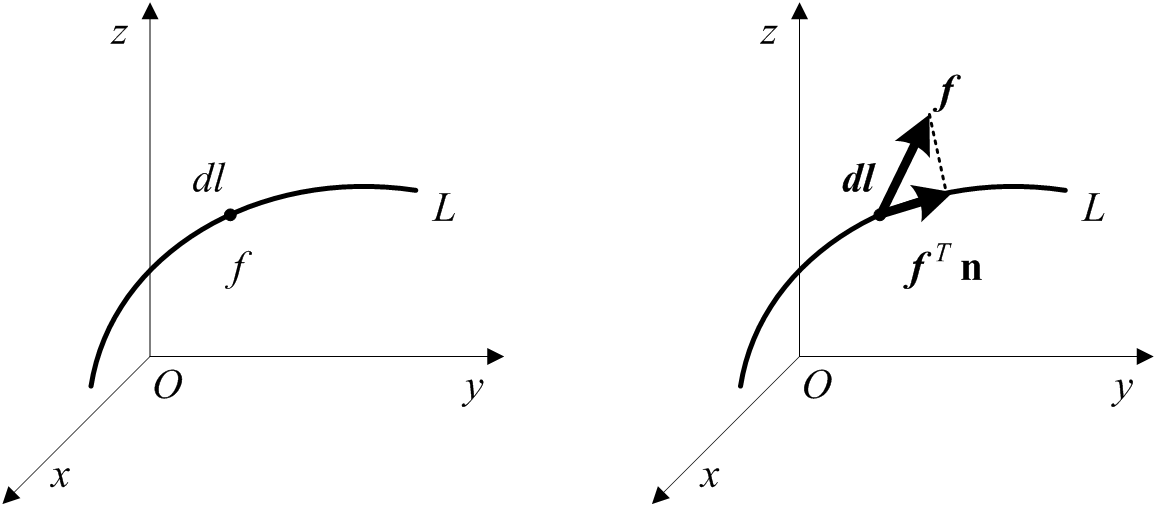
\includegraphics[height=3.5cm]{9.1.png}
\end{figure}

\begin{tcolorbox}
从式子上看,只要看到$dl$的,都是第一类曲线积分,有$dx,dy,dz$单独出现的,就是第二类曲线积分。
\end{tcolorbox}

%============================================================
\subsection{曲线积分的物理意义}

物理上,第一类曲线积分表示一个数量场对一段弧的积分,如绳的质量、非均匀带电曲线的电荷总量等。
第二类曲线积分是对一个矢量场进行环流积分,即求矢量场$\boldsymbol{f}\left( \boldsymbol{p} \right) $在沿某一环流$L$下的环流量。
如果矢量场是力场,则环流积分就是力沿该曲线作的功,如果矢量场是电场,则环流积分就是电势差。

%============================================================
\subsection{计算方法对比}

假设曲线
\[
L:\begin{cases}
	x=x\left( t \right)\\
	y=y\left( t \right)\\
	z=z\left( t \right)\\
\end{cases} \quad t\in \left[ t_1,t_2 \right]
\]
第一类曲线积分和第二类曲线积分:
\begin{align*}
&\begin{cases}
	\int_L{f\left( \boldsymbol{p} \right) dl}\\
	dl=\sqrt{\left( x' \right) ^2+\left( y' \right) ^2+\left( z' \right) ^2}\cdot dt\\
\end{cases} \\
&\Rightarrow \int\limits_L{f\left( \boldsymbol{p} \right) dl}=\int_{t_1}^{t_2}{\left[ f\left( t \right) \cdot \sqrt{\left( x' \right) ^2+\left( y' \right) ^2+\left( z' \right) ^2} \right] dt} \\
&\begin{cases}
	\int_L{\boldsymbol{f}\left( \boldsymbol{p} \right) ^T\boldsymbol{dl}}\\
	\boldsymbol{dl}=\mathbf{n}dl=\left( x'\,\,y'\,\,z' \right) ^Tdt\\
\end{cases} \\
&\Rightarrow \int\limits_L{\boldsymbol{f}\left( \boldsymbol{p} \right) ^T\boldsymbol{dl}}=\int_{t_1}^{t_2}{\left[ P\left( t \right) \cdot x'+Q\left( t \right) \cdot y'+R\left( t \right) \cdot z' \right] dt}
\end{align*}





\newpage
\section{习题}

\begin{exercise}
计算下列曲线积分,并指出是第一类曲线积分还是第二类曲线积分:
\begin{enumerate}
    \item $\int_L{xydx}$,其中$L:x^2+y^2=2x$,$\left( 0,0 \right) \rightarrow \left( 2,0 \right) $上半周。
    \item $\int_L{ydx+zdy+xdz}$,其中$
    L:\begin{cases}
        x^2+y^2=1\\
        x+z=1\\
    \end{cases}
    $,{\it x}轴从正向负看,逆时针一周。
    \item $\int_L{ydl}$,其中$L:\frac{x^2}{25}+\frac{y^2}{9}=1$,{\it x}轴上方部分。
\end{enumerate}
\end{exercise}

解:

1. 只对$dx$积分,即只对{\it x}轴进行积分,所以是第二类曲线积分,曲线$L$可以化为$\left( x-1 \right) ^2+y^2=1$,表示圆心为$\left( 1,0 \right) $、半径为1的圆,曲线化为参数方程求解:
\begin{align*}
&L:\begin{cases}
	x=1+\cos t\\
	y=\sin t\\
\end{cases} \quad t\in \left[ \pi ,0 \right] \\
&\int\limits_L{xydx}=\int_{\pi}^0{\left( 1+\cos t \right) \sin t\cdot d\left( 1+\cos t \right)}=\frac{\pi}{2}
\end{align*}

2. 分别对三个轴积分,所以是第二类曲线积分,曲线化为参数方程求解:
\begin{align*}
&L:\begin{cases}
	x=\cos t\\
	y=\sin t\\
	z=1-\cos t\\
\end{cases} \quad t\in \left[ 0,2\pi \right] \\
&\int\limits_L{ydx+zdy+xdz} \\
&=\int_0^{2\pi}{\sin t\left( -\sin t \right) dt+\left( 1-\cos t \right) \cos tdt+\cos t\sin tdt}=-2\pi
\end{align*}

3. 显然是第一类曲线积分,曲线化为参数方程求解:
\begin{align*}
&L:\begin{cases}
	x=5\cos t\\
	y=3\sin t\\
\end{cases} \quad t\in \left[ 0,\pi \right] \\
&\int\limits_L{ydl}=\int_0^{\pi}{\left[ 3\sin t\cdot \sqrt{\left( -5\sin t \right) ^2+\left( 3\cos t \right) ^2} \right] dt}=9+\frac{75}{4}\mathrm{arc}\sin \frac{4}{5}
\end{align*}

\begin{tcolorbox}
总体思路是将曲线换成参数方程,规划出参数的积分区间。
\end{tcolorbox}

~

\begin{exercise}
求螺旋线
\[
L:\begin{cases}
	x=R\cos t\\
	y=R\sin t\\
	z=kt\\
\end{cases}
\]
在区域$t\in \left[ 0,2\pi \right] $内的长度。
\end{exercise}

解:

这是典型的对弧长的积分,属于第一类曲线积分,可以认为$f\left( \boldsymbol{p} \right) \equiv 1$,于是:
\begin{align*}
\int\limits_L{f\left( \boldsymbol{p} \right) \cdot dl}&=\int_0^{2\pi}{\sqrt{\left( x' \right) ^2+\left( y' \right) ^2+\left( z' \right) ^2}dt} \\
&=\int_0^{2\pi}{\sqrt{\left( -R\sin t \right) ^2+\left( R\cos t \right) ^2+k^2}dt} \\
&=\int_0^{2\pi}{\sqrt{R^2+k^2}dt}=2\pi \sqrt{R^2+k^2}
\end{align*}

~

\begin{exercise}
平面上一半径为R的圆形细线,其中任一点处的线密度为该点到圆周某一固定直径距离的平方,求细线质量。
\end{exercise}

解:

根据题目得到线密度函数$\rho \left( \boldsymbol{p} \right) =y^2$,细线质量为线密度对弧长的积分,也即$\rho \left( \boldsymbol{p} \right) =y^2$在一整圈上的第一类曲线积分,我们只需要计算第一象限积分即可:
\begin{align*}
&M=4\int\limits_L{\rho \left( \boldsymbol{p} \right) \cdot dl}=4\int\limits_L{y^2\cdot dl}=4\int\limits_L{y^2\cdot \sqrt{\left( x' \right) ^2+\left( y' \right) ^2}\cdot dt} \\
&L=\left\{ \left( x,y \right) \middle| 0\leqslant x\leqslant 1,0\leqslant y\leqslant 1,x^2+y^2=1 \right\}
\end{align*}
将曲线转成参数方程求解:
\begin{align*}
&L:\begin{cases}
	x=R\cos t\\
	y=R\sin t\\
\end{cases} \quad t\in \left[ 0,\frac{\pi}{2} \right] \\
&\begin{aligned}
	M&=4\int\limits_L{y^2\cdot \sqrt{\left( x' \right) ^2+\left( y' \right) ^2}\cdot dt} \\
    &=4\int_0^{\frac{\pi}{2}}{R^2\sin ^2t\sqrt{\left( -R\sin t \right) ^2+\left( R\cos t \right) ^2}dt}\\
	&=4R^3\int_0^{\frac{\pi}{2}}{\sin ^2tdt}=2R^3\int_0^{\frac{\pi}{2}}{\left( 1-\cos 2t \right) dt}=\pi R^3\\
\end{aligned}
\end{align*}

~

\begin{exercise}
若向量值函数$\boldsymbol{f}\left( \boldsymbol{p} \right) =\left( y^2\,\,2xy \right) ^T$,计算沿抛物线$y=x^2$从$\left( 0,0 \right) $到$\left( 1,1 \right) $一段弧的曲线积分,若抛物线$y=\sqrt{x},\left( 0,0 \right) \rightarrow \left( 1,1 \right) $,重新计算曲线积分。
\end{exercise}

解:

很显然是第二类曲线积分:
\begin{align*}
&\int\limits_L{\boldsymbol{f}^T\boldsymbol{dl}}=\int_0^1{y^2dx+2xydy}=\int_0^1{\left[ x^4+2x\cdot x^2\cdot 2x \right] dx}=1 \\
&\int\limits_L{\boldsymbol{f}^T\boldsymbol{dl}}=\int_0^1{y^2dx+2xydy}=\int_0^1{\left[ x+2x\cdot \sqrt{x}\cdot \frac{1}{2\sqrt{x}} \right] dx}=1
\end{align*}

~

\begin{exercise}
设二维平面上有力场$\boldsymbol{F}$,方向指向原点,大小与该点到原点的距离成正比,若有质点沿椭圆$\frac{x^2}{a^2}+\frac{y^2}{b^2}=1$逆时针从$\left( a,0 \right) $运动到$\left( 0,b \right) $,求力场对质点作的功。
\end{exercise}

解:

很典型的第二类曲线积分,根据题意,可得力场和曲线:
\begin{align*}
&L:\begin{cases}
	x=a\cos t\\
	y=b\sin t\\
\end{cases} \quad t\in \left[ 0,\frac{\pi}{2} \right] \\
&\boldsymbol{F}\left( \boldsymbol{p} \right) =k\sqrt{x^2+y^2}\left( \begin{array}{c}
	-\frac{x}{\sqrt{x^2+y^2}}\\
	-\frac{y}{\sqrt{x^2+y^2}}\\
\end{array} \right) =\left( \begin{array}{c}
	-kx\\
	-ky\\
\end{array} \right)
\end{align*}
力场作功:
\begin{align*}
W&=\int\limits_L{\boldsymbol{f}\left( \boldsymbol{p} \right) ^T\boldsymbol{dl}}=\int\limits_L{Pdx+Qdy+Rdz}=\int\limits_L{\left( -kx \right) dx+\left( -ky \right) dy} \\
&=\int_0^{\frac{\pi}{2}}{\left[ \left( -ka\cos t \right) \left( -a\sin t \right) +\left( -kb\sin t \right) \left( b\cos t \right) \right] dt} \\
&=k\left( a^2-b^2 \right) \int_0^{\frac{\pi}{2}}{\sin t\cos tdt}=\frac{k}{2}\left( a^2-b^2 \right)
\end{align*}
质点从$\left( a,0 \right) $运动到$\left( 0,b \right) $过程中:
\begin{itemize}
    \item 当$a>b$时,质点在靠近圆心,力场做正功,$W>0$;
    \item 当$a<b$时,质点在远离圆心,力场做负功,$W<0$。
\end{itemize}

~

\begin{exercise}
设曲线
\[
L:\begin{cases}
	x=t\\
	y=t^2\\
	z=t^3\\
\end{cases} \quad t\in \left[ 0,1 \right]
\]
把第二类曲线积分$\int_L{Pdx+Qdy+Rdz}$化为第一类曲线积分。
\end{exercise}

解:

首先观察弧微分:
\begin{align*}
&\because \begin{cases}
	dx=dt\\
	dy=2tdt\\
	dz=3t^2dt\\
\end{cases} \\
&\therefore dl=\sqrt{\left( dx \right) ^2+\left( dy \right) ^2+\left( dz \right) ^2}=\sqrt{1+4t^2+9t^4}\cdot dt
\end{align*}
再看积分:
\begin{align*}
\int\limits_L{Pdx+Qdy+Rdz}&=\int\limits_L{Pdt+Q2tdt+R3t^2dt} \\
&=\int\limits_L{\left( P+Q2t+R3t^2 \right) \cdot dt} \\
&=\int\limits_L{\left( P+Q2t+R3t^2 \right) \cdot \frac{dl}{\sqrt{1+4t^2+9t^4}}} \\
&=\int\limits_L{\frac{P+2xQ+3yR}{\sqrt{1+4y+9y^2}}\cdot dl}
\end{align*}










\chapter{曲面积分}

本章讨论第一类曲面积分和第二类曲面积分。

“第一类曲面积分”是数量值函数对曲面的积分,表示对曲面的累积量。
“第二类曲面积分”是向量值函数对曲面的积分,是两个矢量的内积。

本章要点:
\begin{itemize}
    \item 第一类曲面积分。
    \item 第二类曲面积分。
\end{itemize}

~

\newpage
\section{第一类曲线积分}

本节讨论第一类曲面积分。
所谓“第一类曲面积分”是数量值函数对曲面的积分。

本节要点:
\begin{itemize}
    \item 掌握第一类曲面积分的概念;
    \item 掌握第一类曲面积分的计算,重点掌握曲面微元的计算。
\end{itemize}

%============================================================
\subsection{第一类曲面积分的概念}

\begin{definition}[第一类曲面积分]
若三维空间中有曲面$S$,$f\left( \boldsymbol{p} \right) ,\boldsymbol{p}\in \mathbb{R} ^3$为定义在该空间上的三元数量值函数,若下式极限存在,则称极限值为{\bf $f\left( \boldsymbol{p} \right) $在$S$上积分称为第一类曲面积分},记为$\iint_S{f\left( \boldsymbol{p} \right) ds}$,即:
\[
\iint\limits_S{f\left( \boldsymbol{p} \right) ds}:=\underset{\lambda \rightarrow 0}{\lim}\sum_{i=1}^n{\left[ f\left( \xi _i,\eta _i,\zeta _i \right) \cdot \Delta s_i \right]}
\]
其中:
\begin{itemize}
    \item $f\left( \boldsymbol{p} \right) $:{\bf 被积函数};
    \item $ds$:{\bf 曲面微元};
    \item $S$:{\bf 积分曲面}。
\end{itemize}
\end{definition}

\begin{tcolorbox}
实际定义参考“教材\cite{book1}”,这里是一个简写,总体来讲就是将曲面分片,每片上取一个值和这一小片面积乘积$f\left( \xi _i,\eta _i,\zeta _i \right) \cdot \Delta s_i$,如果和式有极限,则成为$f\left( \boldsymbol{p} \right) $在$S$上有第一类曲面积分。
大致思路和一元函数积分一样。
\end{tcolorbox}

简单说明曲面微元$ds$和{\it xOy}平面投影微元$d\sigma $的关系,这是求解第一类曲面积分的关键。
如果曲面在被积范围内可微,则某点处的曲面微元$ds$与该点处的切面微元$dA$的面积相等。
若曲面由$z=z\left( x,y \right) $显式给出,则切面的法向量为$\boldsymbol{n}=\left( -z_x\,\,-z_y\,\,1 \right) ^T$。
假设法向量和{\it z}轴成角$\theta $,则有:
\[
\cos \theta =\frac{1}{\sqrt{\left( z_x \right) ^2+\left( z_y \right) ^2+1}}
\]
则切面微元$dA$和{\it xOy}平面投影微元$d\sigma $有关系:
\[
d\sigma =\cos \theta \cdot dA=\frac{1}{\sqrt{\left( z_x \right) ^2+\left( z_y \right) ^2+1}}\cdot dA
\]
可得曲面微元$ds$和{\it xOy}平面投影微元$d\sigma $的关系:
\[
ds=\sqrt{\left( z_x \right) ^2+\left( z_y \right) ^2+1}\cdot d\sigma =\sqrt{\left( z_x \right) ^2+\left( z_y \right) ^2+1}\cdot dxdy
\]

\begin{figure}[h]
\centering
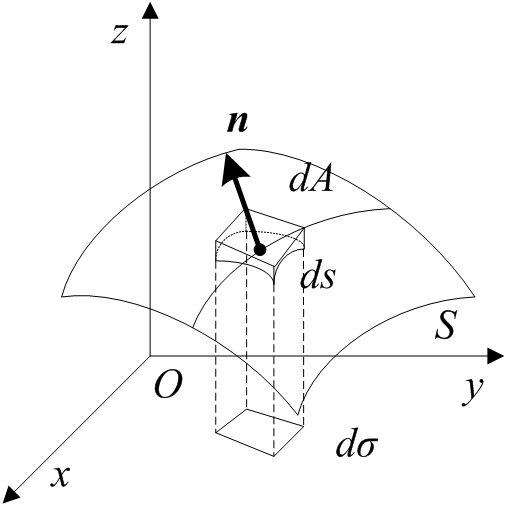
\includegraphics[height=4cm]{10.1.png}
\end{figure}

%============================================================
\subsection{第一类曲面积分的计算}

\begin{theorem}[第一类曲面积分的计算公式]
若$f\left( \boldsymbol{p} \right) $在曲面$S$上连续,$z=z\left( x,y \right) $在$S$上具有一阶连续偏导,则第一类曲面积分的计算公式有:
\begin{align*}
&\iint\limits_S{f\left( \boldsymbol{p} \right) ds}=\iint\limits_D{\left[ f\left( x,y,z\left( x,y \right) \right) \cdot \sqrt{\left( z_x \right) ^2+\left( z_y \right) ^2+1} \right] dxdy} \\
&S=\left\{ \left( x,y,z \right) \middle| x_1\leqslant x\leqslant x_2,y_1\left( x \right) \leqslant y\leqslant y_2\left( x \right) ,z=z\left( x,y \right) \right\} \\
&D=\left\{ \left( x,y \right) \middle| x_1\leqslant x\leqslant x_2,y_1\left( x \right) \leqslant y\leqslant y_2\left( x \right) \right\}
\end{align*}
\end{theorem}

第一类曲面积分的计算关键在于理解曲面微元和投影微元的关系:
\[
ds=\sqrt{\left( z_x \right) ^2+\left( z_y \right) ^2+1}\cdot d\sigma =\sqrt{\left( z_x \right) ^2+\left( z_y \right) ^2+1}\cdot dxdy
\]
通过这个关系,将第一类曲面积分化为二重积分。






\newpage
\section{第二类曲面积分}

本节讨论第二类曲面积分。
所谓“第二类曲面积分”是向量值函数对曲面的积分。

本节要点:
\begin{itemize}
    \item 掌握第二类曲面积分的概念;
    \item 掌握第二类曲面积分的计算,重点掌握积分表达式的内积计算。
\end{itemize}

%============================================================
\subsection{第二类曲面积分的概念}

\begin{definition}[第二类曲面积分]
若三维空间中有曲线$S$,$\mathbf{n}\left( \boldsymbol{p} \right) $为曲面上任一点处的单位法向量,$\boldsymbol{f}\left( \boldsymbol{p} \right) $为定义在该空间上的三元向量值函数,若内积$\boldsymbol{f}\left( \boldsymbol{p} \right) ^T\mathbf{n}\left( \boldsymbol{p} \right) $在$S$上的第一类曲面积分存在,则称此积分值为{\bf $\boldsymbol{f}\left( \boldsymbol{p} \right) $在$S$上的第二类曲面积分},记为$\iint_S{\left[ \boldsymbol{f}\left( \boldsymbol{p} \right) ^T\mathbf{n}\left( \boldsymbol{p} \right) \right] \cdot ds}$,由于$\mathbf{n}\left( \boldsymbol{p} \right) ds=\boldsymbol{ds}$为曲面微元在三个坐标平面的投影,所以更普遍地记作$\iint_S{\boldsymbol{f}\left( \boldsymbol{p} \right) ^T\boldsymbol{ds}}$,即:
\begin{align*}
&\iint\limits_S{\left[ \boldsymbol{f}\left( \boldsymbol{p} \right) ^T\mathbf{n}\left( \boldsymbol{p} \right) \right] \cdot ds}=\iint\limits_S{\boldsymbol{f}\left( \boldsymbol{p} \right) ^T\boldsymbol{ds}} \\
&:=\underset{\lambda \rightarrow 0}{\lim}\sum_{i=1}^n{\left[ \boldsymbol{f}\left( \xi _i,\eta _i,\zeta _i \right) ^T\mathbf{n}\left( \xi _i,\eta _i,\zeta _i \right) \cdot \Delta s_i \right]}
\end{align*}
其中:
\begin{itemize}
    \item $\boldsymbol{f}\left( \boldsymbol{p} \right) $:{\bf 被积函数};
    \item $\mathbf{n}\left( \boldsymbol{p} \right) $:曲面$S$的{\bf 单位法向量};
    \item $\boldsymbol{ds}=\mathbf{n}\left( \boldsymbol{p} \right) ds$:{\bf 有向曲面微元};
    \item $S$:{\bf 积分曲面}。
\end{itemize}
特别地,当$S$为封闭曲面时,记为$\oiint_S{\boldsymbol{f}\left( \boldsymbol{p} \right) ^T\boldsymbol{ds}}$。
\end{definition}

这里要注意,第二类曲面积分是有方向性的,默认方向是曲面的法方向,如果取反方向,则写为:
\[
\iint\limits_{S^-}{\boldsymbol{f}\left( \boldsymbol{p} \right) ^T\boldsymbol{ds}}
\]

%============================================================
\subsection{第二类曲面积分的计算}

\begin{theorem}[第二类曲面积分的计算公式]
我们知道有向曲面微元有:
\begin{align*}
\boldsymbol{ds}&=\mathbf{n}\left( \boldsymbol{p} \right) ds=\frac{\left( -z_x\,\,-z_y\,\,1 \right) ^T}{\sqrt{\left( z_x \right) ^2+\left( z_y \right) ^2+1}} \left[ \sqrt{\left( z_x \right) ^2+\left( z_y \right) ^2+1}\cdot dxdy \right] \\
&=\left( \begin{array}{c}
	-z_x\\
	-z_y\\
	1\\
\end{array} \right) dxdy
\end{align*}
所以向量值函数$\boldsymbol{f}\left( \boldsymbol{p} \right) =\left( P\,\,Q\,\,R \right) ^T$的第二类曲面积分的计算有:
\begin{align*}
\iint\limits_S{\boldsymbol{f}\left( \boldsymbol{p} \right) ^T\boldsymbol{ds}}&=\iint\limits_S{\left( \begin{array}{c}
	P\\
	Q\\
	R\\
\end{array} \right) ^T\left( \begin{array}{c}
	-z_x\\
	-z_y\\
	1\\
\end{array} \right) dxdy} \\
&=\iint\limits_S{\left( -Pz_x-Qz_y+R \right) dxdy}
\end{align*}
\end{theorem}

这里,第二类曲面积分的计算是将有向曲面微元投影到{\it xOy}平面,也可以投影到其他平面,看曲面以什么形式给出。
和第二类曲线积分一样,重点理解被积表达式中的内积。

曲面$S$的单位法向量可写成方向余弦形式$\mathbf{n}=\left( \cos \alpha \,\,\cos \beta \,\,\cos \gamma \right) ^T$,于是积分:
\[
\iint\limits_S{\boldsymbol{f}\left( \boldsymbol{p} \right) ^T\boldsymbol{ds}}=\iint\limits_S{\left( \begin{array}{c}
	P\\
	Q\\
	R\\
\end{array} \right) ^T\left( \begin{array}{c}
	\cos \alpha\\
	\cos \beta\\
	\cos \gamma\\
\end{array} \right) ds}
\]
而又有投影关系:
\begin{align*}
&\cos \alpha \cdot ds=dydz \\
&\cos \beta \cdot ds=dzdx \\
&\cos \gamma \cdot ds=dxdy
\end{align*}
所以第二类曲面积分还可以写为:
\[
\iint\limits_S{\boldsymbol{f}\left( \boldsymbol{p} \right) ^T\boldsymbol{ds}}=\iint\limits_S{Pdydz+Qdzdx+Rdxdy}
\]
这表明$\boldsymbol{f}\left( \boldsymbol{p} \right) $在$S$上的积分可以分解为其三个坐标分量($P,Q,R$)分别对坐标平面({\it yOz}、{\it zOx}和{\it xOy})积分的代数和。






\newpage
\section{两类曲面积分的对比和意义}

本节首先对比两类曲面积分,分析它们的区别,再讨论它们的物理意义。

本节要点:
\begin{itemize}
    \item 理解“对曲面”和“对坐标平面”的含义;
    \item 理解曲面积分的物理意义。
\end{itemize}

%============================================================
\subsection{曲面积分的对比}

将三重积分和两类曲面积分放在一起,
\begin{align*}
&\iiint\limits_V{f\left( \boldsymbol{p} \right) dv} \\
&\iint\limits_S{f\left( \boldsymbol{p} \right) ds} \\
&\iint\limits_S{\boldsymbol{f}\left( \boldsymbol{p} \right) ^T\mathbf{n}\left( \boldsymbol{p} \right) \cdot ds}=\iint\limits_S{\boldsymbol{f}\left( \boldsymbol{p} \right) ^T\boldsymbol{ds}}
\end{align*}
可以看到:
\begin{itemize}
    \item 第一类曲面积分和三重积分的区别只在积分区域,前者是曲面,后者是三维体;
    \item 第一类曲面积分的积分区域是一个曲面,所以又称{\bf 对曲面面积的积分};
    \item 第二类曲面积分又可以写成坐标平面分量的形式,所以又称{\bf 对坐标平面的曲面积分};
    \item 两种曲面积分的区别在于被积函数,第二类曲面积分的被积函数是向量值函数在切面法方向上的投影$\boldsymbol{f}\left( \boldsymbol{p} \right) ^T\mathbf{n}\left( \boldsymbol{p} \right) $,或者说第二类曲面积分的积分表达式是两个向量函数的内积$\boldsymbol{f}\left( \boldsymbol{p} \right) ^T\boldsymbol{ds}$;
    \item 计算方法上,都是化成重积分求解。
\end{itemize}

\begin{tcolorbox}
从式子上看,只要看到$ds$的都是第一类曲面积分,有$dxdy,dydz,dzdx$单独出现的就是第二类曲面积分。
\end{tcolorbox}

%============================================================
\subsection{曲面积分的物理意义}

物理上,第一类曲面积分表示一数量场对曲面的总量,如弧面的质量、非均匀带电球面的电荷总量等。
第二类曲面积分是计算一矢量场对曲面的总通量的问题,如果是电场,则通量就是通过该曲面的电通量,如果是水流,则通量就是流过该曲面的水流量。

举例说明,三维空间中,一个固定方向的流速均匀流速场通过一个垂直平面的流量为$v\cdot S$。
如果平面和流速场方向不一致,则需要引入它们之间的夹角$v\cdot S\cdot \cos \theta $,可以理解为平面在流速场方向的投影,也可以理解为两个矢量的内积$\boldsymbol{v}^T\boldsymbol{S}$。

\begin{figure}[h]
\centering
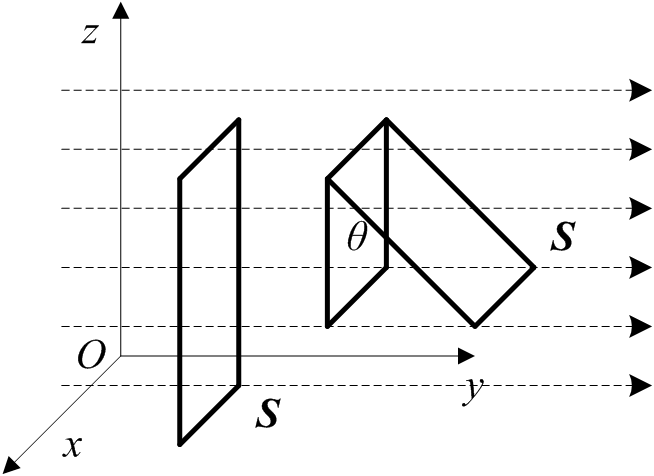
\includegraphics[height=3.5cm]{10.2.png}
\end{figure}

%============================================================
\subsection{计算方法对比}

假设曲面$S=\left\{ \left( x,y,z \right) |x_1\leqslant x\leqslant x_2,y_1\left( x \right) \leqslant y\leqslant y_2\left( x \right) ,z=z\left( x,y \right) \right\} $。
根据给出的曲面方程,投影到{\it xOy}平面。

第一类曲面积分:
\begin{align*}
&\iint\limits_S{f\left( \boldsymbol{p} \right) ds} \qquad ds=\sqrt{\left( z_x \right) ^2+\left( z_y \right) ^2+1}\cdot dxdy \\
&\Downarrow \\
&\iint\limits_S{f\left( \boldsymbol{p} \right) ds}=\iint\limits_D{\left[ f\left( x,y \right) \cdot \sqrt{\left( z_x \right) ^2+\left( z_y \right) ^2+1} \right] dxdy} \\
&D=\left\{ \left( x,y \right) \middle| x_1\leqslant x\leqslant x_2,y_1\left( x \right) \leqslant y\leqslant y_2\left( x \right) \right\}
\end{align*}

第二类曲面积分:
\begin{align*}
&\iint\limits_S{\boldsymbol{f}\left( \boldsymbol{p} \right) ^T\boldsymbol{ds}} \qquad \boldsymbol{ds}=\mathbf{n}\left( \boldsymbol{p} \right) ds=\left( -z_x\,\,-z_y\,\,1 \right) ^Tdxdy \\
&\Downarrow \\
&\iint\limits_S{\boldsymbol{f}\left( \boldsymbol{p} \right) ^T\boldsymbol{ds}}=\iint\limits_S{\left[ -P\left( x,y \right) \cdot z_x-Q\left( x,y \right) \cdot z_y+R\left( x,y \right) \right] dxdy} \\
&D=\left\{ \left( x,y \right) \middle| x_1\leqslant x\leqslant x_2,y_1\left( x \right) \leqslant y\leqslant y_2\left( x \right) \right\}
\end{align*}






\newpage
\section{多元积分总结}

由于多元能产生矢量,所以多元积分分数量值积分和向量值积分,但无论哪个积分,最终结果都是一个标量值。

数量值积分的被积函数是数量值函数,表示数量值对于被积区域的累积,可分为重积分、线积分、面积分,向量值积分的被积函数是向量值函数,表示向量值在有向被积区域内的累积,可分为线积分和面积分。

对于数量值函数:
\begin{table}[h]
\centering
\begin{tabular}{lll}
    \toprule
    名称 & 表达式 & 物理意义\\
    \midrule
    重积分   & $\iiint_V{f\left( \boldsymbol{p} \right) dv}$ & 体质量\\
    曲线积分 & $\int_L{f\left( \boldsymbol{p} \right) dl}$   & 曲线质量\\
    曲面积分 & $\iint_S{f\left( \boldsymbol{p} \right) ds}$  & 曲面质量\\
    \bottomrule
\end{tabular}
\end{table}

对于向量值函数:
\begin{table}[h]
\centering
\begin{tabular}{lll}
    \toprule
    名称 & 表达式 & 物理意义\\
    \midrule
    曲线积分 & $\int_L{\boldsymbol{f}\left( \boldsymbol{p} \right) ^T\boldsymbol{dl}}$  & 矢量场的环流量\\
    曲面积分 & $\iint_S{\boldsymbol{f}\left( \boldsymbol{p} \right) ^T\boldsymbol{ds}}$ & 矢量场的通量\\
    \bottomrule
\end{tabular}
\end{table}






\newpage
\section{习题}

\begin{exercise}
已知球面$x^2+y^2+z^2=R^2$,求包含在柱面$x^2+y^2=Rx$中的部分的面积。
\end{exercise}

解:

基本思路是求解一个区域内曲面的面积。
由于对称性,只计算第一卦限。
首先分析积分区域,得:
\[
S=\left\{ \left( x,y,z \right) \middle| 0\leqslant x\leqslant R,0\leqslant y\leqslant \sqrt{Rx-x^2},z=\sqrt{R^2-x^2-y^2} \right\}
\]
于是面积:
\begin{align*}
&A=4\iint\limits_S{ds}=4\iint\limits_D{\sqrt{1+{z_x}^2+{z_y}^2}dxdy}=4R\iint\limits_D{\frac{1}{\sqrt{R^2-x^2-y^2}}dxdy} \\
&D=\left\{ \left( x,y \right) \middle| 0\leqslant x\leqslant R,0\leqslant y\leqslant \sqrt{Rx-x^2} \right\}
\end{align*}
为计算简单,化为极坐标:
\begin{align*}
&A=4R\iint\limits_D{\frac{r}{\sqrt{R^2-r^2}}drd\theta} \\
&D=\left\{ \left( r,\theta \right) \middle| 0\leqslant \theta \leqslant \frac{\pi}{2},0\leqslant r\leqslant R\cos \theta \right\}
\end{align*}
解得:
\begin{align*}
A&=4R\int_0^{\frac{\pi}{2}}{d\theta \int_0^{R\cos \theta}{\frac{r}{\sqrt{R^2-r^2}}dr}} \\
&=4R\int_0^{\frac{\pi}{2}}{\left( R-R\sin \theta \right) d\theta}=\left( 2\pi -4 \right) R^2
\end{align*}


~

\begin{exercise}
设有流速场$\boldsymbol{v}\left( \boldsymbol{p} \right) =\left( x\,\,y\,\,z \right) $,求通过曲面$S:x^2+y^2+z^2=R^2,z\geqslant 0$的流量。
\end{exercise}

解:

曲面是一个位于原点的球形的上半部分。
大致思路就是构建第二类曲面积分方程,主要是被积函数和积分曲面,然后求解。

首先构建积分方程:
\[
\varPhi =\iint\limits_S{\boldsymbol{v}^T\boldsymbol{ds}}=\iint\limits_S{\left( \begin{array}{c}
	x\\
	y\\
	z\\
\end{array} \right) ^T\left( \begin{array}{c}
	-z_x\\
	-z_y\\
	1\\
\end{array} \right) dxdy}=\iint\limits_S{\left( -xz_x-yz_y+z \right) dxdy}
\]
求解$z_x,z_y$,需要用到隐函数偏导方法,构建隐函数$F\left( x,y,z \right) =x^2+y^2+z^2-R^2$:
\begin{align*}
&z_x=-\frac{F_x}{F_z}=-\frac{x}{z} \\
&z_y=-\frac{F_y}{F_z}=-\frac{y}{z}
\end{align*}
代入得:
\begin{align*}
&\varPhi =\iint\limits_S{\left( \frac{x^2}{z}+\frac{y^2}{z}+z \right) dxdy}=\iint\limits_S{\frac{R^2}{z}dxdy}=\iint\limits_D{\frac{R^2}{\sqrt{R^2-x^2-y^2}}dxdy} \\
&D=\left\{ \left( x,y \right) \middle| -R\leqslant x\leqslant R,-\sqrt{R^2-x^2}\leqslant y\leqslant \sqrt{R^2-x^2} \right\}
\end{align*}
转换到极坐标求解:
\begin{align*}
\varPhi &=\iint\limits_D{\frac{R^2}{\sqrt{R^2-r^2}}rdrd\theta}=R^2\int_0^{2\pi}{d\theta \int_0^R{\frac{r}{\sqrt{R^2-r^2}}dr}} \\
&=R^2\int_0^{2\pi}{Rd\theta}=2\pi R^3
\end{align*}










\chapter{微积分基本定理和场论}

本章介绍多元函数积分的三个重要公式,Green公式、Gauss公式和Stokes公式,及梯度、散度和旋度。
这三个公式是物理的基本公式,可以认为是多元函数微积分在物理方面的基础,是前几章在物理方面的应用。

本章要点:
\begin{itemize}
    \item Green公式。
    \item Gauss公式。
    \item Stokes公式。
    \item 保守场。
    \item 微积分基本定理。
\end{itemize}

~

\newpage
\section{格林Green公式}

本节讨论格林Green公式。
Green公式是二维平面的二重积分和边界积分的关系,是后续两个公式的“预热”。

本节要点:
\begin{itemize}
    \item 掌握Green公式的概念。
\end{itemize}

%============================================================
\subsection{格林Green公式的概念}

\begin{definition}[Green公式]
假设二维平面中有单连通区域$D$,其正向边界$L$分段光滑,$\boldsymbol{f}\left( \boldsymbol{p} \right) =\left( P\,\,Q \right) ^T$是定义在二维平面上的向量值函数,且$P,Q$在$D$上有一阶连续偏导数,则有:
\[
\oint\limits_L{\boldsymbol{f}^T\boldsymbol{dl}}=\oint\limits_L{Pdx+Qdy}=\iint\limits_D{\left( \frac{\partial Q}{\partial x}-\frac{\partial P}{\partial y} \right) dxdy}
\]
上述公式称为{\bf Green公式}。
若假设$D$为复连通区域,其正向外边界为$L_1$,正向内边界为$L_2$,则有:
\[
\oint\limits_{L_1}{\boldsymbol{f}^T\boldsymbol{dl}}+\oint\limits_{L_2}{\boldsymbol{f}^T\boldsymbol{dl}}=\iint\limits_D{\left( \frac{\partial Q}{\partial x}-\frac{\partial P}{\partial y} \right) dxdy}
\]
\end{definition}

\begin{figure}[h]
\centering
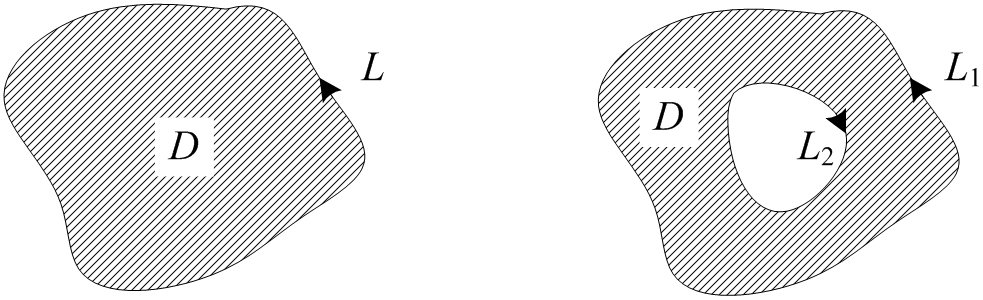
\includegraphics[height=2.5cm]{11.1.png}
\end{figure}






\newpage
\section{高斯Gauss公式和散度}

本节介绍Gauss公式。

本节要点:
\begin{itemize}
    \item 掌握Gauss公式的概念;
    \item 理解Gauss公式的物理意义;
    \item 掌握散度的概念;
    \item 理解散度的物理意义。
\end{itemize}

%============================================================
\subsection{Gauss公式的概念}

\begin{definition}[Gauss公式]
假设三维空间中有单连通区域$V$,其外侧边界$S$分片光滑,$\boldsymbol{f}\left( \boldsymbol{p} \right) =\left( P\,\,Q\,\,R \right) ^T$是定义在三维空间上的向量值函数,且$P,Q,R$在$V$上有一阶连续偏导数,则有:
\begin{align*}
&\oiint\limits_S{\boldsymbol{f}^T\boldsymbol{ds}}=\oiint\limits_S{Pdydz+Qdzdx+Rdxdy}= \\
&\iiint\limits_V{\left( \frac{\partial P}{\partial x}+\frac{\partial Q}{\partial y}+\frac{\partial R}{\partial z} \right) dv}
\end{align*}
上述公式称为{\bf Gauss公式}。
\end{definition}

%============================================================
\subsection{Gauss公式的物理意义}

Gauss公式左边代表一个矢量场对于一个封闭曲面的总通量:
\begin{itemize}
    \item $\boldsymbol{f}^T\boldsymbol{ds}$:通量微元,或者说是矢量场在曲面微元形成的通量;
    \item $\oiint_S$:对整个封闭曲面的总累积量;
    \item $\oiint_S{\boldsymbol{f}^T\boldsymbol{ds}}=0$:通量为0,表示流入流出该空间的量相抵消;
    \item $\oiint_S{\boldsymbol{f}^T\boldsymbol{ds}}>0$:表示有东西流出该区域;
    \item $\oiint_S{\boldsymbol{f}^T\boldsymbol{ds}}<0$:表示有东西流入该区域。
\end{itemize}

Gauss公式右边代表这个封闭曲面中源或者汇:
\begin{itemize}
    \item $\left( \frac{\partial P}{\partial x}+\frac{\partial Q}{\partial y}+\frac{\partial R}{\partial z} \right) dv$:该点处的源或者汇;
    \item $\iiint_V$:整个区域中的所有的源或汇;
    \item $\iiint_V{\left( \frac{\partial P}{\partial x}+\frac{\partial Q}{\partial y}+\frac{\partial R}{\partial z} \right) dv}=0$:表示区域内既无源也无汇;
    \item $\iiint_V{\left( \frac{\partial P}{\partial x}+\frac{\partial Q}{\partial y}+\frac{\partial R}{\partial z} \right) dv}>0$:表示区域内有源;
    \item $\iiint_V{\left( \frac{\partial P}{\partial x}+\frac{\partial Q}{\partial y}+\frac{\partial R}{\partial z} \right) dv}<0$:表示区域内有汇。
\end{itemize}

\begin{tcolorbox}
Gauss公式的物理意义显而易见,整个公式描述一个矢量场。
左边从其对区域边界的作用效果的角度描述,即矢量场在边界造成的通量。
右边从其在区域内的总的发散或汇聚的量的角度描述。
\end{tcolorbox}

%============================================================
\subsection{散度的概念}

如果将曲面无限缩小,就是该点的发散或汇聚的量。

\begin{definition}[散度]
若三维空间中有矢量值函数$\boldsymbol{f}\left( \boldsymbol{p} \right) $在有向封闭曲面$S$内的积分$\oiint_S{\boldsymbol{f}^T\boldsymbol{ds}}$,设$\lambda =\max \left\{ \left\| \boldsymbol{p}_0-\boldsymbol{p} \right\| \right\} $表示该曲面的包围体中最远点到目标点$\boldsymbol{p}_0$的距离,设$V$为包围体的体积,若当$\lambda \rightarrow 0$时,极限$\underset{\lambda \rightarrow 0}{\lim}\frac{\oiint_S{\boldsymbol{f}\left( \boldsymbol{p}_0 \right) ^T\boldsymbol{ds}}}{V}$存在,则称该极限为{\bf $\boldsymbol{f}\left( \boldsymbol{p} \right) $在$\boldsymbol{p}_0$点的散度},记为$\mathrm{div}\boldsymbol{f}$,即:
\[
\mathrm{div}\boldsymbol{f}=\underset{\lambda \rightarrow 0}{\lim}\frac{\oiint\limits_S{\boldsymbol{f}^T\boldsymbol{ds}}}{V}
\]
\end{definition}

根据Gauss公式可以得到散度的计算公式:
\[
\mathrm{div}\boldsymbol{f}=\underset{V\rightarrow \boldsymbol{p}_0}{{\lim}}\frac{1}{V}\iiint\limits_V{\left( \frac{\partial P}{\partial x}+\frac{\partial Q}{\partial y}+\frac{\partial R}{\partial z} \right) dv}=\frac{\partial P}{\partial x}+\frac{\partial Q}{\partial y}+\frac{\partial R}{\partial z}
\]
反过来,运用散度公式,Gauss公式可以表示为:
\[
\oiint\limits_S{\boldsymbol{f}^T\boldsymbol{ds}}=\iiint\limits_V{\mathrm{div}\boldsymbol{f}\cdot dv}
\]
注意:
\begin{itemize}
    \item 散度只能针对矢量场,数量场没有“流”,所以也就没有散度这个概念;
    \item 散度是该点流出汇入的量的体密度,根据Gauss公式,是该点沿各坐标轴的流出汇入程度的代数和;
    \item 一个矢量场的散度是一个数量场,可以处处为0,表示该场没有流出点和汇入点,即该矢量场是个{\bf 无源场},如磁场。
\end{itemize}

\begin{tcolorbox}
Gauss公式的物理意义更显而易见,一封闭曲面包围下的通量等于该包围下所有点的散度和。
\end{tcolorbox}

~

\begin{example}
设有矢量场$\boldsymbol{f}\left( \boldsymbol{p} \right) =\left( xy^2 \quad ye^z \quad x\ln \left( 1+z^2 \right) \right) $,求该向量场的散度场,并求在点$\left( 1,1,0 \right) $处的散度。
\end{example}

解:
\begin{align*}
&\mathrm{div}\boldsymbol{f}=\frac{\partial P}{\partial x}+\frac{\partial Q}{\partial y}+\frac{\partial R}{\partial z}=y^2+e^z+x\frac{2z}{1+z^2} \\
&\left. \mathrm{div}\boldsymbol{f} \right|_{\left( 1,1,0 \right)}=1+1+1\cdot \frac{0}{1}=2
\end{align*}

%============================================================
\subsection{散度的量纲和物理意义}

结合物理量的单位的理解散度的物理意义。
假设有流速场$\boldsymbol{v}$,量纲为$\mathrm{m}\cdot \mathrm{s}^{-1}$,表示该点的流速:

\begin{table}[h]
\centering
\begin{tabular}{lll}
    \toprule
    表达式 & 量纲\\
    \midrule
    $\boldsymbol{v}$ & $\mathrm{m}\cdot \mathrm{s}^{-1}$\\
    $\oiint_S{\boldsymbol{v}^T\boldsymbol{ds}}$ & $\mathrm{m}^3\cdot \mathrm{s}^{-1}$\\
    $\mathrm{div}\boldsymbol{v}=\underset{\lambda \rightarrow 0}{\lim}\frac{\oiint_S{\boldsymbol{v}^T\boldsymbol{ds}}}{V}$ & $\mathrm{s}^{-1}$\\
    \bottomrule
\end{tabular}
\end{table}

$\mathrm{div}\boldsymbol{v}$的量纲没有$\mathrm{m}$,是$\mathrm{s}^{-1}$,说明散度作为空间上的一个“点”,本身不承载尺度信息,只反映了该点的流速的程度。
如果我们做一个体积分再加上一个时间积分,就是一段时间内流出或流入一个体的总流量。
\[
\int_{t_1}^{t_2}{\left( \iiint\limits_V{\mathrm{div}\boldsymbol{v}\cdot dv} \right) dt}
\]

%============================================================
\subsection{散度和微分算子}

在第七章中介绍了向量微分算子$\nabla =\left( \frac{\partial}{\partial x}\,\,\frac{\partial}{\partial y}\,\,\frac{\partial}{\partial z} \right) ^T$。
根据散度公式和微分算子,可以做纯数学上的抽象:
\begin{align*}
&\because \begin{cases}
	\mathrm{div}\boldsymbol{f}=\frac{\partial P}{\partial x}+\frac{\partial Q}{\partial y}+\frac{\partial R}{\partial z}\\
	\nabla ^T\boldsymbol{f}=\left( \begin{array}{c}
	\frac{\partial}{\partial x}\\
	\frac{\partial}{\partial y}\\
	\frac{\partial}{\partial z}\\
\end{array} \right) ^T\left( \begin{array}{c}
	P\\
	Q\\
	R\\
\end{array} \right) =\frac{\partial P}{\partial x}+\frac{\partial Q}{\partial y}+\frac{\partial R}{\partial z}\\
\end{cases} \\
&\therefore \mathrm{div}\boldsymbol{f}=\nabla ^T\boldsymbol{f}
\end{align*}
即散度可以记为微分算子和矢量场的内积,于是Gauss公式还可以写为:
\[
\oiint\limits_S{\boldsymbol{f}^T\boldsymbol{ds}}=\iiint\limits_V{\left( \nabla ^T\boldsymbol{f} \right) dv}
\]






\newpage
\section{斯托克斯Stokes公式和旋度}

本节介绍Stokes公式。

本节要点:
\begin{itemize}
    \item 掌握Stokes公式的概念;
    \item 理解Stokes公式的物理意义;
    \item 掌握旋度的概念;
    \item 理解旋度的物理意义。
\end{itemize}

%============================================================
\subsection{Stokes公式的概念}

\begin{definition}[Stokes公式]
假设三维空间中有分片光滑曲面$S$,其边界$L$分段光滑,两者方向符合右手定则,即右手四指表示曲线$L$方向,大拇指的指向和曲面$S$的方向一致,$\boldsymbol{f}\left( \boldsymbol{p} \right) =\left( P\,\,Q\,\,R \right) ^T$是定义在三维空间上的向量值函数,且$P,Q,R$在$S$上有一阶连续偏导数,则有:
\begin{align*}
&\oint\limits_L{\boldsymbol{f}^T\boldsymbol{dl}}=\oint\limits_L{Pdx+Qdy+Rdz}= \\
&\iint\limits_S{\left( \frac{\partial R}{\partial y}-\frac{\partial Q}{\partial z} \right) dydz+\left( \frac{\partial P}{\partial z}-\frac{\partial R}{\partial x} \right) dzdx+\left( \frac{\partial Q}{\partial x}-\frac{\partial P}{\partial y} \right) dxdy}
\end{align*}
称为{\bf Stokes公式}。
\end{definition}

Green公式可视为Stokes的二维特例,之后一般情况下将不作讨论。

%============================================================
\subsection{Stokes公式的物理意义}

Stokes公式左边代表一个矢量场沿一个闭合曲线一周产生的环流量:
\begin{itemize}
    \item $\boldsymbol{f}^T\boldsymbol{dl}$:环流微量,表示沿封闭曲线方向产生的微作用力;
    \item $\oint_L$:环曲线一周的累积效果;
    \item $\oint_L{\boldsymbol{f}^T\boldsymbol{dl}}=0$:表示绕该闭合曲线一周不产生效果;
    \item $\oint_L{\boldsymbol{f}^T\boldsymbol{dl}}>0$:表示绕该闭合曲线一周会产生某种“正”效果,可以理解为“加速”效果;
    \item $\oint_L{\boldsymbol{f}^T\boldsymbol{dl}}<0$:表示绕该闭合曲线一周会产生某种“负”效果,可以理解为“减速”效果。
\end{itemize}

\begin{tcolorbox}
Stokes公式右边的物理意义暂不考虑。到这里,只需要理解“环流量”,更深入的物理意义在给出旋度这个概念后再分析。
\end{tcolorbox}

%============================================================
\subsection{旋度的概念}

如果将环无限缩小,就是在该点的自旋一周产生的环流效果。

\begin{definition}[旋度]
若三维空间中有矢量值函数$\boldsymbol{f}\left( \boldsymbol{p} \right) $在有向闭合曲线$L$内的积分$\oint_L{\boldsymbol{f}^T\boldsymbol{dl}}$,设$\lambda =\max \left\{ \left\| \boldsymbol{p}_0-\boldsymbol{p} \right\| \right\} $表示该曲线围成的曲面上最远点到目标点$\boldsymbol{p}_0$的距离,设$S$为包围的曲面的面积,若当$\lambda \rightarrow 0$时,极限$\underset{\lambda \rightarrow 0}{\lim}\frac{\oint_L{\boldsymbol{f}\left( \boldsymbol{p}_0 \right) ^T\boldsymbol{dl}}}{S}$存在,则称该极限为{\bf $\boldsymbol{f}\left( \boldsymbol{p} \right) $在$\boldsymbol{p}_0$点的旋度},记为$\mathbf{rot}\boldsymbol{f}$,即:
\[
\mathbf{rot}\boldsymbol{f}=\underset{\lambda \rightarrow 0}{\lim}\frac{\oint\limits_L{\boldsymbol{f}\left( \boldsymbol{p}_0 \right) ^T\boldsymbol{dl}}}{S}
\]
\end{definition}

根据Stokes公式得到旋度计算公式:
\begin{align*}
\mathbf{rot}\boldsymbol{f}&=\underset{L\rightarrow M}{\lim}\frac{\iint\limits_S{\left( \frac{\partial R}{\partial y}-\frac{\partial Q}{\partial z} \right) dydz+\left( \frac{\partial P}{\partial z}-\frac{\partial R}{\partial x} \right) dzdx+\left( \frac{\partial Q}{\partial x}-\frac{\partial P}{\partial y} \right) dxdy}}{S} \\
&=\underset{L\rightarrow M}{\lim}\frac{1}{S}\iint\limits_S{\left( \begin{array}{c}
	\frac{\partial R}{\partial y}-\frac{\partial Q}{\partial z}\\
	\frac{\partial P}{\partial z}-\frac{\partial R}{\partial x}\\
	\frac{\partial Q}{\partial x}-\frac{\partial P}{\partial y}\\
\end{array} \right) ^T\left( \begin{array}{c}
	dydz\\
	dzdx\\
	dxdy\\
\end{array} \right)} \\
&=\underset{L\rightarrow M}{\lim}\frac{1}{S}\iint\limits_S{\left( \begin{array}{c}
	\frac{\partial R}{\partial y}-\frac{\partial Q}{\partial z}\\
	\frac{\partial P}{\partial z}-\frac{\partial R}{\partial x}\\
	\frac{\partial Q}{\partial x}-\frac{\partial P}{\partial y}\\
\end{array} \right) ^T\boldsymbol{ds}} \\
&=\left( \begin{array}{c}
	\frac{\partial R}{\partial y}-\frac{\partial Q}{\partial z}\\
	\frac{\partial P}{\partial z}-\frac{\partial R}{\partial x}\\
	\frac{\partial Q}{\partial x}-\frac{\partial P}{\partial y}\\
\end{array} \right) =\left| \begin{matrix}
	\mathbf{i}&		\mathbf{j}&		\mathbf{k}\\
	\frac{\partial}{\partial x}&		\frac{\partial}{\partial y}&		\frac{\partial}{\partial z}\\
	P&		Q&		R\\
\end{matrix} \right|
\end{align*}
运用旋度公式,Stokes公式可以表示为:
\[
\oint\limits_L{\boldsymbol{f}^T\boldsymbol{dl}}=\iint\limits_S{\left( \mathbf{rot}\boldsymbol{f} \right) ^T\boldsymbol{ds}}
\]

注意:
\begin{itemize}
    \item 旋度只能针对矢量场,数量场没有旋度这个概念;
    \item 旋度描述了一矢量场在某点的旋转程度(可以理解为角速度);
    \item 该旋转程度可以分解对应到各个坐标轴的旋转程度,所以旋度的结果是一个矢量场;
    \item 一个矢量场的旋度可以处处为0,表示该场没有任何旋转,即该矢量场是个{\bf 无旋场},如点电荷产生的电场。
\end{itemize}

\begin{tcolorbox}
矢量场可以没有旋度,如静止的点电荷产生的电场,电力线“直直地”发散出去,空间任意一点“左右两侧”的场强方向和大小一致,不会使得该点处的电荷发生转动。
再如,一个均匀的、直的河流,水流“笔直地”向前流,没有旋转,但如果河道弯曲,流水沿河道方向有拐弯,产生了涡流,在该涡流处的叶子会发生“转动”。
所以,旋度的“旋”,表示该点处“左右”两侧流速“相反”,会使该点“旋转”。
\end{tcolorbox}

%============================================================
\subsection{旋度的量纲和物理意义}

结合物理单位,假设流速场$\boldsymbol{v}$:

\begin{table}[h]
\centering
\begin{tabular}{lll}
    \toprule
    表达式 & 量纲\\
    \midrule
    $\boldsymbol{v}$ & $\mathrm{m}\cdot \mathrm{s}^{-1}$\\
    $\oint_L{\boldsymbol{v}^T\boldsymbol{dl}}$ & $\mathrm{m}^2\cdot \mathrm{s}^{-1}$\\
    $\mathbf{rot}\boldsymbol{v}=\underset{\lambda \rightarrow 0}{\lim}\frac{\oint_L{\boldsymbol{v}^T\boldsymbol{dl}}}{S}$ & $\mathrm{s}^{-1}$\\
    \bottomrule
\end{tabular}
\end{table}

旋度表示空间里一点的自转角速度。
如果一个曲面上每点自转角速度累加起来不为零,则整个曲面也会转起来,整个曲面的自旋可以通过环流量度量。

\begin{tcolorbox}
Stokes公式的物理意义在于,其描述的是一个矢量场,确切地讲是描述一个矢量场在一个曲面上造成的自旋程度。
公式右边表示曲面上各个点自旋程度的累积,左边则是这种自旋在边界造成的环流量。
\end{tcolorbox}

%============================================================
\subsection{旋度和微分算子}

根据旋度公式和微分算子$\nabla =\left( \frac{\partial}{\partial x}\,\,\frac{\partial}{\partial y}\,\,\frac{\partial}{\partial z} \right) ^T$,可以做纯数学上的抽象:
\begin{align*}
&\because \begin{cases}
	\mathbf{rot}\boldsymbol{f}=\left| \begin{matrix}
	\mathbf{i}&		\mathbf{j}&		\mathbf{k}\\
	\frac{\partial}{\partial x}&		\frac{\partial}{\partial y}&		\frac{\partial}{\partial z}\\
	P&		Q&		R\\
\end{matrix} \right|\\
	\nabla \times \boldsymbol{f}=\left( \begin{array}{c}
	\frac{\partial}{\partial x}\\
	\frac{\partial}{\partial y}\\
	\frac{\partial}{\partial z}\\
\end{array} \right) \times \left( \begin{array}{c}
	P\\
	Q\\
	R\\
\end{array} \right) =\left| \begin{matrix}
	\mathbf{i}&		\mathbf{j}&		\mathbf{k}\\
	\frac{\partial}{\partial x}&		\frac{\partial}{\partial y}&		\frac{\partial}{\partial z}\\
	P&		Q&		R\\
\end{matrix} \right|\\
\end{cases} \\
&\therefore \mathbf{rot}\boldsymbol{f}=\nabla \times \boldsymbol{f}
\end{align*}
即旋度可以记为微分算子和矢量场的外积,于是Stokes公式可以写为:
\[
\oint\limits_L{\boldsymbol{f}^T\boldsymbol{dl}}=\iint\limits_S{\left( \nabla \times \boldsymbol{f} \right) ^T\boldsymbol{ds}}
\]






\newpage
\section{度、微分算子和拉普拉斯算子}

梯度作用于标量场,得到其关于变化率的一个矢量场:
\[
\mathbf{grad}f=\nabla f=\left( \frac{\partial f}{\partial x} \quad \frac{\partial f}{\partial y} \quad \frac{\partial f}{\partial z} \right) ^T
\]
散度作用于矢量场,得到其关于流出汇入程度的一个标量场:
\[
\mathrm{div}\boldsymbol{f}=\nabla ^T\boldsymbol{f}=\frac{\partial P}{\partial x}+\frac{\partial Q}{\partial y}+\frac{\partial R}{\partial z}
\]
旋度作用于矢量场,得到其关于旋转速度的一个矢量场:
\[
\mathbf{rot}\boldsymbol{f}=\nabla \times \boldsymbol{f}=\left| \begin{matrix}
	\mathbf{i}&		\mathbf{j}&		\mathbf{k}\\
	\frac{\partial}{\partial x}&		\frac{\partial}{\partial y}&		\frac{\partial}{\partial z}\\
	P&		Q&		R\\
\end{matrix} \right|=\left( \begin{array}{c}
	\frac{\partial R}{\partial y}-\frac{\partial Q}{\partial z}\\
	\frac{\partial P}{\partial z}-\frac{\partial R}{\partial x}\\
	\frac{\partial Q}{\partial x}-\frac{\partial P}{\partial y}\\
\end{array} \right)
\]
特别地,标量场的梯度可以再次作散度,记作$\nabla ^2f$,即:
\[
\nabla ^2f=\nabla ^T\left( \nabla f \right) =\left( \begin{array}{c}
	\frac{\partial}{\partial x}\\
	\frac{\partial}{\partial y}\\
	\frac{\partial}{\partial z}\\
\end{array} \right) ^T\left( \begin{array}{c}
	\frac{\partial f}{\partial x}\\
	\frac{\partial f}{\partial y}\\
	\frac{\partial f}{\partial z}\\
\end{array} \right) =\frac{\partial ^2f}{\partial x^2}+\frac{\partial ^2f}{\partial y^2}+\frac{\partial ^2f}{\partial z^2}
\]
我们称$\nabla ^2$为{\bf 拉普拉斯算子},记作$\Delta $,即:
\[
\Delta :=\nabla ^2=\frac{\partial ^2}{\partial x^2}+\frac{\partial ^2}{\partial y^2}+\frac{\partial ^2}{\partial z^2}
\]

拉普拉斯算子作用于标量场,首先得到变化率的矢量场,再得到该矢量场的汇入流出情况。
最终,拉普拉斯算子等价于得到一个标量场的最高点和最低点。






\newpage
\section{曲线积分的路径无关性和保守场}

\begin{theorem}
设$D$为平面上的单连通区域,$\boldsymbol{f}\left( \boldsymbol{p} \right) =\left( P\,\,Q \right) ^T$是定义在二维平面上的向量值函数,且$P,Q$在$D$上有一阶连续偏导数,则下面4个命题等价:
\begin{enumerate}[label=\Roman*.]
    \item $D$内封闭曲线$L$上有$\oint_L{\boldsymbol{f}^T\boldsymbol{dl}}=0$;
    \item $\oint_L{\boldsymbol{f}^T\boldsymbol{dl}}=0$在$D$内与路径无关;
    \item $D$中必有数量值函数$g\left( \boldsymbol{p} \right) $,满足$\frac{\partial g}{\partial x}=P,\frac{\partial g}{\partial y}=Q$,即有全微分$dg=Pdx+Qdy$;
    \item $D$内每一点满足$\frac{\partial Q}{\partial x}=\frac{\partial P}{\partial y}$。
\end{enumerate}
\end{theorem}

以上:
\begin{itemize}
    \item 命题I和IV的等价性由Green公式体现;
    \item 命题III和IV综合即为二阶混偏相等定理。
\end{itemize}

\begin{theorem}
假设三维空间中有一单连通区域,$\boldsymbol{f}\left( \boldsymbol{p} \right) =\left( P\,\,Q\,\,R \right) ^T$是定义在该区域上的向量值函数,且$P,Q,R$在该区域上有一阶连续偏导数,则下面4个命题等价:
\begin{enumerate}[label=\Roman*.]
    \item 区域内任意封闭曲线$L$上有$\oint_L{\boldsymbol{f}^T\boldsymbol{dl}}=0$;
    \item $\oint_L{\boldsymbol{f}^T\boldsymbol{dl}}=0$在区域内与路径无关;
    \item 区域内必有数量值函数$g\left( \boldsymbol{p} \right) $有全微分,且满足$dg=Pdx+Qdy+Rdz$;
    \item 区域内每点满足$\frac{\partial R}{\partial y}=\frac{\partial Q}{\partial z},\frac{\partial P}{\partial z}=\frac{\partial R}{\partial x},\frac{\partial Q}{\partial x}=\frac{\partial P}{\partial y}$,即
    \[
    \left| \begin{matrix}
    	\mathbf{i}&		\mathbf{j}&		\mathbf{k}\\
    	\frac{\partial}{\partial x}&		\frac{\partial}{\partial y}&		\frac{\partial}{\partial z}\\
    	P&		Q&		R\\
    \end{matrix} \right|=0
    \]
\end{enumerate}
\end{theorem}

\begin{definition}
如果一个矢量场中,在任何区域内沿任何曲线的第二类曲线积分与路径无关,只与曲线的起点和终点有关,称该矢量场为{\bf 保守场}。
如果一个矢量场是保守场,则该场的旋度为0,$\nabla \times \boldsymbol{f}=0$,同时该场必然是一个标量场的梯度,即$\nabla g=\boldsymbol{f}$,$g$称为$\boldsymbol{f}$的{\bf 势函数},$\boldsymbol{f}$也称为{\bf 有势场}。
\end{definition}

也即这4个概念等价:保守场$\Leftrightarrow $无旋场$\Leftrightarrow $梯度场$\Leftrightarrow $有势场。






\newpage
\section{微积分基本定理}

本节在纯数学的抽象上讨论Gauss公式和Stokes公式的意义。
首先引入微分的外积、外微分形式和外微分算子,将两个公式进行外微分化,得到微积分基本定理的统一公式。
最后在外微分的角度重新考察一下三个度。

本节要点:
\begin{itemize}
    \item 了解微分外积的概念;
    \item 了解外微分形式的概念;
    \item 了解统一公式。
\end{itemize}

%============================================================
\subsection{微分的外积}

在一元积分中,有方向的概念,即$\int_a^b{fdx}=-\int_b^a{fdx}$。
在第二类曲线积分和第二类曲面积分中,也有方向的概念。
第二类曲线积分中的方向是曲线的切线的方向,第二类曲面积分中的方向是曲面的切平面的法方向。
但公式中的如$dxdy$本身不承担方向的正负性,即$dxdy=dydx$。
方向及其正反性都由切线和切平面决定。
讨论微积分基本定理、挖掘三个公式的共同点时,需要把这个方向的“正反性”让$dxdy$承担,即我们需要定义一个概念,或者说一个运算规则,使得$dx\bigcirc dy=-dy\bigcirc dx$。

\begin{definition}[微分外积]
规定一种微分的乘法运算,记为$\land $,使得:
\begin{itemize}
    \item $dx\land dy=-dy\land dx$
    \item $dx\land dx=0$
\end{itemize}
满足这两条的微分乘法称为{\bf 微分的外积}。同时称$dxdy$为{\bf 微分的内积}。
\end{definition}

\begin{tcolorbox}
微分的内积和外积,可以类比于矢量的内积和外积。
\end{tcolorbox}

%============================================================
\subsection{外微分形式}

\begin{definition}[外微分形式]
设$P,Q,R$均为定义在三维空间的三元数量值函数,且在三维空间的某区域$V$内可微,我们定义如下概念。

称它们各自对三个坐标轴微分的积的代数和为{\bf $V$上的一个一阶外微分形式},记为$\omega $,即:
\[
\omega =Pdx+Qdy+Rdz
\]
$P,Q,R$称为这个{\bf 一阶外微分形式$\omega $的系数}。

称它们各自对三个坐标平面的外积微分的积的代数和为{\bf $V$上的一个二阶外微分形式},同样可以记为$\omega $,即:
\[
\omega =Pdy\land dz+Qdz\land dx+Rdx\land dy
\]
$P,Q,R$称为这个{\bf 二阶外微分形式$\omega $的系数}。

设$f$在三维空间$V$内可微,则称它对$V$上的外积形式的体积微元为{\bf $V$上的一个三阶外微分形式},记为$\omega $,即:
\[
\omega =fdx\land dy\land dz
\]
$f$称为这个{\bf 三阶外微分形式$\omega $的系数}。

特别地,我们称这个可微函数$f$本身为{\bf $V$上的一个零阶外微分形式}。

\end{definition}

%============================================================
\subsection{外微分算子}

对外微分形式$\omega $定义外微分算子$d$。

对于零阶外微分形式,即函数$f$本身,外微分算子为$f$的全微分:
\[
d\omega =df=\frac{\partial f}{\partial x}dx+\frac{\partial f}{\partial y}dy+\frac{\partial f}{\partial z}dz
\]

对于一阶外微分形式$\omega =Pdx+Qdy+Rdz$,外微分算子为:
\begin{align*}
&d\omega =dP\land dx+dQ\land dy+dR\land dz \\
&\because \left\{ \begin{aligned}
	dP\land dx&=\left( \frac{\partial P}{\partial x}dx+\frac{\partial P}{\partial y}dy+\frac{\partial P}{\partial z}dz \right) \land dx\\
	&=\frac{\partial P}{\partial y}dy\land dx+\frac{\partial P}{\partial z}dz\land dx\\
	dQ\land dy&=\left( \frac{\partial Q}{\partial x}dx+\frac{\partial Q}{\partial y}dy+\frac{\partial Q}{\partial z}dz \right) \land dy\\
	&=\frac{\partial Q}{\partial x}dx\land dy+\frac{\partial Q}{\partial z}dz\land dy\\
	dR\land dz&=\left( \frac{\partial R}{\partial x}dx+\frac{\partial R}{\partial y}dy+\frac{\partial R}{\partial z}dz \right) \land dz\\
	&=\frac{\partial R}{\partial x}dx\land dz+\frac{\partial R}{\partial y}dy\land dz\\
\end{aligned} \right. \\
&\therefore d\omega =\left( \frac{\partial R}{\partial y}-\frac{\partial Q}{\partial z} \right) dy\land dz+\left( \frac{\partial P}{\partial z}-\frac{\partial R}{\partial x} \right) dz\land dx \\
& \qquad \qquad +\left( \frac{\partial Q}{\partial x}-\frac{\partial P}{\partial y} \right) dx\land dy
\end{align*}

对于二阶外微分形式$\omega =Pdy\land dz+Qdz\land dx+Rdx\land dy$,外微分算子为:
\begin{align*}
&d\omega =dP\land dy\land dz+dQ\land dz\land dx+dR\land dx\land dy \\
&\because \left\{ \begin{aligned}
	dP\land dy\land dz&=\left( \frac{\partial P}{\partial x}dx+\frac{\partial P}{\partial y}dy+\frac{\partial P}{\partial z}dz \right) \land dy\land dz\\
	&=\frac{\partial P}{\partial y}\land dx\land dy\land dz\\
	dQ\land dz\land dx&=\left( \frac{\partial Q}{\partial x}dx+\frac{\partial Q}{\partial y}dy+\frac{\partial Q}{\partial z}dz \right) \land dz\land dx\\
	&=\frac{\partial Q}{\partial y}dx\land dy\land dz\\
	dR\land dx\land dy&=\left( \frac{\partial R}{\partial x}dx+\frac{\partial R}{\partial y}dy+\frac{\partial R}{\partial z}dz \right) \land dx\land dy\\
	&=\frac{\partial R}{\partial z}dx\land dy\land dz\\
\end{aligned} \right. \\
&\therefore d\omega =\left( \frac{\partial P}{\partial x}+\frac{\partial Q}{\partial y}+\frac{\partial R}{\partial z} \right) dx\land dy\land dz
\end{align*}

对于三阶外微分形式$\omega =fdx\land dy\land dz$,外微分算子为:
\begin{align*}
&d\omega =dfdx\land dy\land dz \\
&\because df=\frac{\partial f}{\partial x}dx+\frac{\partial f}{\partial y}dy+\frac{\partial f}{\partial z}dz \\
&\therefore d\omega =\left( \frac{\partial f}{\partial x}dx+\frac{\partial f}{\partial y}dy+\frac{\partial f}{\partial z}dz \right) \land dx\land dy\land dz=0
\end{align*}

%============================================================
\subsection{统一公式}

将Gauss公式和Stokes公式写成外微分形式:
\begin{align*}
&\oiint\limits_S{Pdy\land dz+Qdz\land dx+Rdx\land dy} \\
& \qquad \qquad \qquad \qquad =\iiint\limits_V{\left( \frac{\partial P}{\partial x}+\frac{\partial Q}{\partial y}+\frac{\partial R}{\partial z} \right) dx\land dy\land dz} \\
&\oint\limits_L{Pdx+Qdy+Rdz}=\iint\limits_S{\left( \frac{\partial R}{\partial y}-\frac{\partial Q}{\partial z} \right) dy\land dz+\left( \frac{\partial P}{\partial z}-\frac{\partial R}{\partial x} \right) dz\land dx} \\
& \qquad \qquad \qquad \qquad +\left( \frac{\partial Q}{\partial x}-\frac{\partial P}{\partial y} \right) dx\land dy
\end{align*}
进一步采用外微分算子可以写成:
\begin{align*}
&\oiint\limits_S{\omega}=\iiint\limits_V{d\omega} \\
&\oint\limits_L{\omega}=\iint\limits_S{d\omega}
\end{align*}
Gauss公式和Stokes公式有共同点,左边是对外微分形式在区域边界的积分,右边是对其外微分算子在该区域的积分。

\begin{theorem}[微积分基本定理的统一公式]
设某$n$维空间内有一封闭区域$\varOmega $,$\varOmega $上有$n$阶外微分形式$\omega $满足其系数为定义在$\varOmega $上的可微数量值函数,$\omega $对应有外微分算子$d\omega $,有:
\[
\oint\limits_{d\varOmega}{\omega}=\iint\limits_{\varOmega}{d\omega}
\]
\end{theorem}

统一公式说明,如果空间中有一个光滑场,则其在对考察区域的边界的作用(即方程的左边),等于该场的源在该区域内的累积(即方程的右边)。
从纯粹公式来看,并不刻意区分场和源的先后问题。
从右向左看,说明源导致一个场;但从左向右看,场必然汇到一个源。
考虑一个球体,电磁场流入球体表面,则必然在内部形成一个负电荷。






\newpage
\section{扩展的假想}

到上一节,多元函数积分学算是结束了。如果不考虑下篇的级数,整个微积分可以说是结束了。

本节讨论一些有趣的话题,算是对微积分这个学习过程中一开始挖下的坑进行填补。
当然,这个填坑是我假想的,并没有严格的数学证明。

%============================================================
\subsection{外积交换时符号的来源}

矢量和微分都有内积和外积:
\begin{align*}
&\boldsymbol{a}^T\boldsymbol{b}=\boldsymbol{b}^T\boldsymbol{a} \\
&\boldsymbol{a}\times \boldsymbol{b}=-\boldsymbol{b}\times \boldsymbol{a} \\
&dxdy=dydx \\
&dx\land dy=-dy\land dx
\end{align*}
“外积”交换时产生负号,是源于我们对外积的定义,还是外积的某种必然属性?

首先考察矢量外积。
由外积的定义发现,负号来源于矢量的方向性,确切来讲,是方向中的“正反性”。
矢量是带有方向的量,这个方向中的“正反性”,体现在外积中就是交换公式中出现的负号。
同样,微分外积的交换公式中的负号也是体现方向“正反性”的体现。
切线有往前和往后之分,切面有上侧下侧(或者说左右侧、前后侧)之分,还是源于矢量的方向性。

在物理上,这个正反性代表着积可以使某个量增大,或者减小,也即这个结果不是一个单一的数量,其作用效果也不是单方面的,而是有着两种截然相反的效果。
数学上,方向的正反性源于一维坐标的正反性。
如果一维坐标里,只有正方向这一个方向,那么最基本的数学运算里只能剩下加法,不会有减法。
所以说,一维坐标的“负向”(或者说负数)是引入减法的必然结果。只有扩充了负向(也即负数),实数才能对减法封闭。

顺着这个思路,实数加法也有“内外”之分,可以定义:
\[
a\oplus b=-b\oplus a
\]
其实,这就是减法,而且还满足:
\[
a\oplus a=0
\]
可见,对于带有方向的一维坐标来讲,有“内加”和“外加”,而减法,就可以说是“外加”。

更进一步说,一物理量只要是矢量,必然有一种运算符合交换后出现负号这个要求,好比顺着不同的“方向”去做同一件事,会得到相反的结果。

%============================================================
\subsection{负数的矢量性和一维矢量}

接着上面的讨论,负数是数量还是矢量?
从数学的学习来看,负数是一个数量,因为它是实数。
但根据上面的讨论,负数似乎带有一定的矢量概念,至少它有矢量的那种正反性。

更深入的问题是二维矢量有没有外积?
如果依照微积分中对外积的定义,二维矢量是没有外积的,因为这样的行列式是不存在的:
\[
\boldsymbol{a}\times \boldsymbol{b}=\left( \begin{array}{c}
	x_{\boldsymbol{a}}\\
	y_{\boldsymbol{a}}\\
\end{array} \right) \times \left( \begin{array}{c}
	x_{\boldsymbol{b}}\\
	y_{\boldsymbol{b}}\\
\end{array} \right) =\left| \begin{matrix}
	\mathbf{i}&		\mathbf{j}\\
	x_{\boldsymbol{a}}&		y_{\boldsymbol{a}}\\
	x_{\boldsymbol{b}}&		y_{\boldsymbol{b}}\\
\end{matrix} \right|
\]
虽然从线性代数的角度看二维矢量是有外积的:
\[
\boldsymbol{a}\times \boldsymbol{b}=\left( \begin{array}{c}
	x_{\boldsymbol{a}}\\
	y_{\boldsymbol{a}}\\
\end{array} \right) \times \left( \begin{array}{c}
	x_{\boldsymbol{b}}\\
	y_{\boldsymbol{b}}\\
\end{array} \right) =x_{\boldsymbol{a}}y_{\boldsymbol{b}}-y_{\boldsymbol{a}}x_{\boldsymbol{b}}
\]
从Green公式来看,它是Stokes公式的二维特例,那么Green公式右边出现的必然是二维矢量的旋度。
从这点看来二维矢量的外积确实应该存在。
再进一步的问题,一维有没有矢量?
如果有,一维矢量的外积是什么?

先看第二个问题,二维矢量的外积,因为这个问题是第一个问题的起源。
Stokes公式的二维化:
\begin{align*}
&\oint\limits_L{\boldsymbol{f}^T\boldsymbol{dl}} \\
&=\iint\limits_S{\left( \frac{\partial R}{\partial y}-\frac{\partial Q}{\partial z} \right) dydz+\left( \frac{\partial P}{\partial z}-\frac{\partial R}{\partial x} \right) dzdx+\left( \frac{\partial Q}{\partial x}-\frac{\partial P}{\partial y} \right) dxdy} \\
&\begin{cases}
	z\equiv 0,dz=0\\
	R\left( x,y,z \right) \equiv 0,\frac{\partial R}{\partial x}=\frac{\partial R}{\partial y}=\frac{\partial R}{\partial z}=0\\
\end{cases}
\end{align*}
于是:
\[
\oint\limits_L{\boldsymbol{f}^T\boldsymbol{dl}}=\iint\limits_S{\left( \frac{\partial Q}{\partial x}-\frac{\partial P}{\partial y} \right) dxdy}
\]
这提醒我们,二维矢量外积的方法是虚拟一个{\it z}轴,并使之恒等于0。

\begin{definition}[二维矢量外积]
设二维矢量$\boldsymbol{a}=\left( x_{\boldsymbol{a}}\,\,y_{\boldsymbol{a}} \right) ^T,\boldsymbol{b}=\left( x_{\boldsymbol{b}}\,\,y_{\boldsymbol{b}}  \right) ^T$,令其对应的三维矢量$\boldsymbol{c}=\left( x_{\boldsymbol{a}}\,\,y_{\boldsymbol{a}}\,\,0  \right) ^T,\boldsymbol{d}=\left( x_{\boldsymbol{b}}\,\,y_{\boldsymbol{b}}\,\,0 \right) ^T$的外积
\[
\boldsymbol{c}\times \boldsymbol{d}=\left( \begin{array}{c}
	x_{\boldsymbol{a}}\\
	y_{\boldsymbol{a}}\\
	0\\
\end{array} \right) \times \left( \begin{array}{c}
	x_{\boldsymbol{b}}\\
	y_{\boldsymbol{b}}\\
	0\\
\end{array} \right) =\left| \begin{matrix}
	\mathbf{i}&		\mathbf{j}&		\mathbf{k}\\
	x_{\boldsymbol{a}}&		x_{\boldsymbol{b}}&		0\\
	y_{\boldsymbol{a}}&		y_{\boldsymbol{b}}&		0\\
\end{matrix} \right|=\left( \begin{array}{c}
	0\\
	0\\
	x_{\boldsymbol{a}}y_{\boldsymbol{b}}-y_{\boldsymbol{a}}x_{\boldsymbol{b}}\\
\end{array} \right)
\]
的$\mathbf{k}$分量$x_{\boldsymbol{a}}y_{\boldsymbol{b}}-y_{\boldsymbol{a}}x_{\boldsymbol{b}}$规定为{\bf 两个二维矢量$\boldsymbol{a},\boldsymbol{b}$的外积},即
\[
\boldsymbol{a}\times \boldsymbol{b}=\left( \begin{array}{c}
	x_{\boldsymbol{a}}\\
	y_{\boldsymbol{a}}\\
\end{array} \right) \times \left( \begin{array}{c}
	x_{\boldsymbol{b}}\\
	y_{\boldsymbol{b}}\\
\end{array} \right) =x_{\boldsymbol{a}}y_{\boldsymbol{b}}-y_{\boldsymbol{a}}x_{\boldsymbol{b}}
\]
而且依然满足:
\begin{align*}
&\boldsymbol{a}\times \boldsymbol{b}=-\boldsymbol{b}\times \boldsymbol{a} \\
&\boldsymbol{a}\times \left( \boldsymbol{b}+\boldsymbol{c} \right) =\boldsymbol{a}\times \boldsymbol{b}+\boldsymbol{a}\times \boldsymbol{c} \\
&\boldsymbol{a}\times \boldsymbol{a}=0
\end{align*}
\end{definition}

根据这个定义回头再看Green公式:
\begin{align*}
&\because \oint\limits_L{\boldsymbol{f}^T\mathbf{dl}}=\iint\limits_S{\left( \nabla \times \boldsymbol{f} \right) ^T\boldsymbol{ds}} \\
&\because \begin{cases}
	\nabla \times \boldsymbol{f}=\left( \begin{array}{c}
	\frac{\partial}{\partial x}\\
	\frac{\partial}{\partial y}\\
\end{array} \right) \times \left( \begin{array}{c}
	P\\
	Q\\
\end{array} \right) =\frac{\partial Q}{\partial x}-\frac{\partial P}{\partial y}\\
	\boldsymbol{ds}=dxdy\\
\end{cases} \\
&\therefore \oint\limits_L{\boldsymbol{f}^T\mathbf{dl}}=\iint\limits_S{\left( \frac{\partial Q}{\partial x}-\frac{\partial P}{\partial y} \right) dxdy}
\end{align*}
可见Stokes公式推导出Green公式非常自然。

但随之而来的问题是,二维矢量的外积是矢量还是数量?
如果承认了是数量就否认了矢量外积依然是矢量,如果承认了是矢量,那就承认数量也是矢量(即承认$x_{\boldsymbol{a}}y_{\boldsymbol{b}}-y_{\boldsymbol{a}}x_{\boldsymbol{b}}$是一个矢量)。
这是“负数是数量还是矢量”这一问题的延续。
也就是说,只要定义了二维矢量的外积,就必然要回答负数是数量还是矢量。
为了不破坏旋度的完美性,我们决定承认二维矢量的外积是矢量,也即承认$x_{\boldsymbol{a}}y_{\boldsymbol{b}}-y_{\boldsymbol{a}}x_{\boldsymbol{b}}$是一个矢量。为此我们需要定义一维矢量。

\begin{definition}[一维矢量]
规定$\mathbb{R} $中的元素是{\bf 一维矢量},采用矢量形式记为$\boldsymbol{a}$,大小为其绝对值$\left| \boldsymbol{a} \right|$,方向只取正负两个方向,并规定正方向是沿着x轴变大的方向,反方向是沿{\it x}轴变小的方向。
同样借助扩展维度的方法规定{\bf 一维矢量的外积}:
\[
\boldsymbol{c}\times \boldsymbol{d}=\left( \begin{array}{c}
	x_{\boldsymbol{a}}\\
	0\\
	0\\
\end{array} \right) \times \left( \begin{array}{c}
	x_{\boldsymbol{b}}\\
	0\\
	0\\
\end{array} \right) =\left| \begin{matrix}
	\mathbf{i}&		\mathbf{j}&		\mathbf{k}\\
	x_{\boldsymbol{a}}&		0&		0\\
	x_{\boldsymbol{b}}&		0&		0\\
\end{matrix} \right|=\left( \begin{array}{c}
	0\\
	0\\
	0\\
\end{array} \right) =\mathbf{0}
\]
得到一维矢量的外积始终是0,而且依然满足外积的运算法则:
\begin{align*}
&\boldsymbol{a}\times \boldsymbol{b}=-\boldsymbol{b}\times \boldsymbol{a} \\
&\boldsymbol{a}\times \left( \boldsymbol{b}+\boldsymbol{c} \right) =\boldsymbol{a}\times \boldsymbol{b}+\boldsymbol{a}\times \boldsymbol{c} \\
&\boldsymbol{a}\times \boldsymbol{a}=0
\end{align*}
\end{definition}

%============================================================
\subsection{一维空间中的度}

顺着上面的定义,将三个度的定义扩充到一维向量空间:
\[
\begin{cases}
	f=f\left( x \right)\\
	\boldsymbol{f}=\left( \begin{array}{c}
	P\\
	0\\
	0\\
\end{array} \right) =f\\
\end{cases} \Rightarrow \quad \begin{cases}
	\nabla f=\left( \frac{\partial f}{\partial x} \right) =\frac{df}{dx}\\
	\nabla ^T\boldsymbol{f}=\frac{\partial P}{\partial x}=\frac{df}{dx}\\
	\nabla \times \boldsymbol{f}=0\\
\end{cases}
\]
一维矢量空间的梯度和散度是一个意思,都是一元函数的导数,几何上是切线的斜率,这个斜率可正可负。
斜率值可以看成传统意义上的数量,此时相当于作散度;也可以继续看成一维矢量,此时相当于作梯度。

\begin{tcolorbox}
可以认为,一维空间中只有一个度——导数。
或者说,一元函数中导数的概念对应了三维空间中向量值函数的三个度的概念。
所以,在一元函数微积分中,对一个一元函数的考察除了导数就没有其他的方法了。
\end{tcolorbox}

我们在一维空间有了梯度、散度和旋度,我们用这些概念考察一维空间的Gauss公式和Stokes公式。

先看Gauss公式:
\[
\oiint\limits_S{\boldsymbol{f}^T\boldsymbol{ds}}=\iiint\limits_V{\left( \nabla ^T\boldsymbol{f} \right) dv}
\]
在一维空间中:
\begin{itemize}
    \item $\iiint_V{\left( \frac{\partial P}{\partial x}+\frac{\partial Q}{\partial y}+\frac{\partial R}{\partial z} \right) dv}$:对应$\int_L{\frac{\partial P}{\partial x}dx}$,其中$L:\left\{ x \middle| x\in \left[ a,b \right] \right\} ,\frac{\partial P}{\partial x}=f'\left( x \right) $,于是可以写为$\int_a^b{f'\left( x \right) dx}$;
    \item $S$:对应区间的两个端点$a,b$;
    \item $\oiint_S{\boldsymbol{f}^T\boldsymbol{ds}}$:表示在边界的通量,这里,边界只有$a,b$两个端点,于是有$\oiint_S{\boldsymbol{f}^T\boldsymbol{ds}}=\boldsymbol{f}\left( a \right) +\boldsymbol{f}\left( b \right) $,由于端点是左边端点,所以根据一维矢量的几何意义,有$\boldsymbol{f}\left( a \right) =-f\left( a \right) $,同样道理$\boldsymbol{f}\left( b \right) =f\left( b \right) $。
\end{itemize}
综合以上3点,我们可以得到一维空间中Gauss公式:
\[
f\left( b \right) -f\left( a \right) =\int_a^b{f'\left( x \right) dx}
\]
即牛顿莱布尼兹公式。

再考察Stokes公式:
\[
\oint\limits_L{\boldsymbol{f}^T\boldsymbol{dl}}=\iint\limits_S{\left( \nabla \times \boldsymbol{f} \right) ^T\boldsymbol{ds}}
\]
左边的$L$为一元函数区间的一个来回,即$L:\left\{ x \middle| x\in \left[ a,b \right] \right\} \cup \left\{ x \middle| x\in \left[ b,a \right] \right\} $,即:
\[
\oint\limits_L{\boldsymbol{f}^T\boldsymbol{dl}}=\int_a^b{f\left( x \right) dx}+\int_b^a{f\left( x \right) dx}=0
\]
右边:
\[
\iint\limits_S{\left( \nabla \times \boldsymbol{f} \right) ^T\boldsymbol{ds}}=\iint\limits_S{\left( \left( \frac{\partial}{\partial x} \right) \times \left( P \right) \right) ^T\mathbf{ds}}=\iint\limits_S{\mathbf{0}^T\boldsymbol{ds}}=0
\]
Stokes公式依然成立。

\begin{tcolorbox}
可见,由于一维空间中三个度的退化,Green公式、Gauss公式、Stokes公式都将退化成牛顿莱布尼兹公式。
\end{tcolorbox}

%============================================================
\subsection{再论散度和旋度的物理意义}

根据之前的分析,我们可以进一步理解散度和旋度。
设空间中有一个封闭区域,内部有一个源(或数个源),以某种方式形成一个矢量场,则这个矢量场对区域边界有两个作用:
\begin{itemize}
	\item “瞄着”区域边界的作用,造成边界膨胀的效果,就是散度要描述的;
	\item “切着”区域边界的作用,造成区域自旋的效果,就是旋度要描述的。
\end{itemize}

如果这个源本身不带有自旋,可能对边界没有“切向”作用,如点电荷产生的电场。
如果这个源本身在旋转,则可能对边界起到旋转作用。
想象一个水桶,底部有一个漏点,桶里的水流入该漏点并绕着漏点发生旋转,水流场可以认为是一个矢量场。
如果围着漏点,放置一根圆形的橡皮筋,则这根橡皮筋一方面受到水流冲击有缩小的趋势,另一方面会顺着涡流的旋转而旋转。
这就是散度和旋度。
如果这个水桶放在赤道上,则这个漏点不产生旋涡,就相当于一个没有自旋的矢量场。

%============================================================
\subsection{梯度散度旋度之外的度}

梯度,散度,旋度:
\begin{align*}
&\mathbf{grad}f=\nabla f=\left( \frac{\partial f}{\partial x}\,\,\frac{\partial f}{\partial y}\,\,\frac{\partial f}{\partial z} \right) ^T \\
&\mathrm{div}\boldsymbol{f}=\nabla ^T\boldsymbol{f}=\frac{\partial P}{\partial x}+\frac{\partial Q}{\partial y}+\frac{\partial R}{\partial z} \\
&\mathbf{rot}\boldsymbol{f}=\nabla \times \boldsymbol{f}=\left| \begin{matrix}
	\mathbf{i}&		\mathbf{j}&		\mathbf{k}\\
	\frac{\partial}{\partial x}&		\frac{\partial}{\partial y}&		\frac{\partial}{\partial z}\\
	P&		Q&		R\\
\end{matrix} \right|=\left( \begin{array}{c}
	\frac{\partial R}{\partial y}-\frac{\partial Q}{\partial z}\\
	\frac{\partial P}{\partial z}-\frac{\partial R}{\partial x}\\
	\frac{\partial Q}{\partial x}-\frac{\partial P}{\partial y}\\
\end{array} \right)
\end{align*}

0、一、二阶外微分形式的外微分算子运算:
\begin{align*}
&\begin{cases}
	\omega =f\\
	d\omega =\frac{\partial f}{\partial x}dx+\frac{\partial f}{\partial y}dy+\frac{\partial f}{\partial z}dz\\
\end{cases} \\
&\begin{cases}
	\omega =Pdx+Qdy+Rdz\\
	d\omega =\left( \frac{\partial R}{\partial y}-\frac{\partial Q}{\partial z} \right) dy\land dz+\left( \frac{\partial P}{\partial z}-\frac{\partial R}{\partial x} \right) dz\land dx+\left( \frac{\partial Q}{\partial x}-\frac{\partial P}{\partial y} \right) dx\land dy\\
\end{cases} \\
&\begin{cases}
	\omega =Pdy\land dz+Qdz\land dx+Rdx\land dy\\
	d\omega =\left( \frac{\partial P}{\partial x}+\frac{\partial Q}{\partial y}+\frac{\partial R}{\partial z} \right) dx\land dy\land dz\\
\end{cases}
\end{align*}

对比发现:
\begin{itemize}
    \item “0阶外微分形式的外微分算子运算”对应“梯度”;
    \item “一阶外微分形式的外微分算子运算”对应“旋度”;
    \item “二阶外微分形式的外微分算子运算”对应“散度”。
\end{itemize}
从外微分的角度看,三维空间不可能再产生其他的度,因为三阶外微分形式的外微分算子运算为0。
或者从数量场和矢量场的相互转换的角度分析:
\begin{itemize}
    \item “数量场、矢量场”的运算:梯度;
    \item “矢量场、数量场”的运算:散度;
    \item “矢量场、矢量场”的运算:旋度;
    \item “数量场、数量场”的运算:没有这样的运算,或类比三阶外微分形式的外微分算子运算为0,即得到的数量场处处为0。
\end{itemize}
从两类场的转化角度看,也不可能有其他的度了。

\begin{tcolorbox}
更严格地讲,是三维矢量(即一阶张量)限制了度的产生,如果考察更多维的空间,或者即便在三维空间中,放开对张量的一阶限制,应该会产生额外的度。
\end{tcolorbox}

%============================================================
\subsection{Gauss公式和数量守恒}

Gauss公式结合麦克斯韦方程可以写为:
\[
\begin{cases}
	\oiint_S{\boldsymbol{f}^T\boldsymbol{ds}}=\iiint\limits_V{\left( \nabla ^T\boldsymbol{f} \right) dv}\\
	\oiint_S{\boldsymbol{E}^T\boldsymbol{ds}}=\frac{q}{\varepsilon _0}\\
	\nabla ^T\boldsymbol{E}=\frac{\rho}{\varepsilon _0\varepsilon _r}\\
\end{cases} \Rightarrow \quad \oiint\limits_S{\boldsymbol{E}^T\boldsymbol{ds}}=\varepsilon _r\iiint\limits_V{\left( \nabla ^T\boldsymbol{E} \right) \cdot dv}=\frac{q}{\varepsilon _0}
\]
从麦克斯韦的电场方程来看,Gauss公式的左边的矢量场表示电场,右边的矢量场的散度表示电荷密度。

\begin{tcolorbox}
{\bf 数量场守恒猜想}:如果一个矢量场及其散度满足Gauss公式描述的相互关系,则其散度所指的那个数量场必守恒。这就是Gauss公式的数量守恒猜想。
\end{tcolorbox}

%============================================================
\subsection{矢量内积和数量守恒}

上面讨论了Gauss公式和数量守恒。
其实矢量的内积运算,就其目的来说,最终是为了引出Gauss公式。
公式里两个地方用到了内积,左边的矢量场和有向面积微元的内积,右边有向微分算子和矢量场的内积。

如果说Gauss公式体现了数量场守恒,则是通过矢量的内积运算表示这个守恒律。
所以,矢量的内积运算是数量守恒的必然结果。
也就是如果你相信数量守恒,则在数学上必须定义一种矢量之间的运算表示为:
\[
\boldsymbol{a}^T\boldsymbol{b}=x_{\boldsymbol{a}}x_{\boldsymbol{b}}+y_{\boldsymbol{a}}y_{\boldsymbol{b}}+z_{\boldsymbol{a}}z_{\boldsymbol{b}}
\]
至于称为“点积”、“内积”还是张三李四积都可以。
或者说,如果你穿越到了某个平行宇宙,发现那边也有矢量,但是很奇怪:
\[
\boldsymbol{a}^T\boldsymbol{b}\ne x_{\boldsymbol{a}}x_{\boldsymbol{b}}+y_{\boldsymbol{a}}y_{\boldsymbol{b}}+z_{\boldsymbol{a}}z_{\boldsymbol{b}}
\]
这就说明那个平行宇宙不遵循数量场守恒。

%============================================================
\subsection{Stokes公式和矢量守恒}

麦克斯韦方程左边是表示电场的环流效果,代表在一个环形上正在产生(或消耗)电能,右边对应着表示磁场的变化,代表磁能的减弱(或增强),结合Stokes公式可写成:
\[
\begin{cases}
	\oint_L{\boldsymbol{f}^T\boldsymbol{dl}}=\iint\limits_S{\left( \nabla \times \boldsymbol{f} \right) ^T\boldsymbol{ds}}\\
	\oint_L{\boldsymbol{E}^T\boldsymbol{dl}}=-\iint\limits_S{\left( \frac{\partial \boldsymbol{B}}{\partial t} \right) ^T\boldsymbol{ds}}\\
	\nabla \times \boldsymbol{E}=-\frac{\partial \boldsymbol{B}}{\partial t}\\
\end{cases} \Rightarrow \quad \oint\limits_L{\boldsymbol{E}^T\boldsymbol{dl}}=\iint\limits_S{\left( \nabla \times \boldsymbol{E} \right) ^T\boldsymbol{ds}}
\]
表示如果一个矢量场能造成一个涡流场(即环流量不为0的矢量场),则矢量场损失的量必然是涡流场的量。

\begin{tcolorbox}
{\bf 矢量场守恒猜想}:如果一个矢量场及其旋度满足Stokes公式描述的关系,则这两个矢量场构成守恒关系。
这就是Stokes公式的矢量守恒猜想。
\end{tcolorbox}

%============================================================
\subsection{矢量外积和矢量守恒}

读任何一本微积分的书,你会发现,矢量外积就是给Stokes公式准备的。
从外积的定义开始,到讲述Stokes公式或者旋度之前,就没说起过外积。
Stokes中旋度表示一个守恒的矢量场。

和矢量内积一样,我们同样也可以认为,矢量外积是矢量守恒的必然结果。
如果你相信矢量守恒,则必须定义:
\[
\boldsymbol{a}\times \boldsymbol{b}=\left( \begin{array}{c}
	x_{\boldsymbol{a}}\\
	y_{\boldsymbol{a}}\\
	z_{\boldsymbol{a}}\\
\end{array} \right) \times \left( \begin{array}{c}
	x_{\boldsymbol{b}}\\
	y_{\boldsymbol{b}}\\
	z_{\boldsymbol{b}}\\
\end{array} \right) =\left| \begin{matrix}
	\mathbf{i}&		\mathbf{j}&		\mathbf{k}\\
	x_{\boldsymbol{a}}&		y_{\boldsymbol{a}}&		z_{\boldsymbol{a}}\\
	x_{\boldsymbol{b}}&		y_{\boldsymbol{b}}&		z_{\boldsymbol{b}}\\
\end{matrix} \right|=\left( \begin{array}{c}
	y_{\boldsymbol{a}}z_{\boldsymbol{b}}-z_{\boldsymbol{a}}y_{\boldsymbol{b}}\\
	z_{\boldsymbol{a}}x_{\boldsymbol{b}}-x_{\boldsymbol{a}}z_{\boldsymbol{b}}\\
	x_{\boldsymbol{a}}y_{\boldsymbol{b}}-y_{\boldsymbol{a}}x_{\boldsymbol{b}}\\
\end{array} \right)
\]
同样,如果某个平行宇宙矢量外积不是这个样子,这就说明那个平行宇宙不遵循矢量场守恒。

\begin{tcolorbox}
或者更大胆一点,矢量的内积和外积是不是三维一阶张量的必然结果?
\end{tcolorbox}

%============================================================
\subsection{守恒和超距作用}

上面讨论了数量场和矢量场的守恒。
一个场的增减,必然会在另一处有相反的增减,或者在其区域边界体现出来。
那么这种守恒,或者变化的空间传递,能够超距作用,还是需要时间传播。

从Gauss公式出发:
\[
\oiint\limits_S{\boldsymbol{f}^T\boldsymbol{ds}}=\iiint\limits_V{\left( \nabla ^T\boldsymbol{f} \right) dv}
\]
空间里,区域$V$中的一个源($\nabla ^T\boldsymbol{f}$)无论是不是在另一个区域中产生对应的源,都会在该区域$V$边界$S$产生效应$\oiint_S{\boldsymbol{f}^T\boldsymbol{ds}}$。
这个效应跟能不能,或者需不需要考虑,产生相对应的源没有关系。
或者说,无论区域$V$中的源要不要在另一个区域产生对应源,都会经过边界$S$。
基于这点,我们可以认为,超距作用,至少对于守恒的数量场是不存在的。
同样分析可以认为,超距作用对于守恒的矢量场也是不存在的。

从Stokes公式的角度看:
\[
\oint\limits_L{\boldsymbol{f}^T\boldsymbol{dl}}=\iint\limits_S{\left( \nabla \times \boldsymbol{f} \right) ^T\boldsymbol{ds}}
\]
如果既要承认超距作用又要矢量守恒,则矢量场必然会发生突变。
相当于磁场$\boldsymbol{B}$在时间上会出现间断点,即在那个时间点$\frac{\partial \boldsymbol{B}}{\partial t}$不存在。
所以如果你既要承认超距作用又要矢量守恒,则从Stokes公式来讲,必然有一个矢量场不是光滑的。

综合来讲,如果一个物理量守恒,它就不可能具有超距属性。
或者说,这个宇宙中,“守恒”和“超距”,你只能选择其一。










\chapter{无穷级数}

本章讨论级数。
所谓无穷级数,就是一个无穷的、有规则的序列的和,所以一般省略“无穷”,直接称级数。

本章先讨论常数项级数,即一般项是固定值的级数,对应后面要介绍的函数项级数。
常数项级数是讨论函数项级数的基础。

本章要点:
\begin{itemize}
    \item 常数项无穷级数。
    \item 函数项级数。
\end{itemize}

~

\newpage
\section{常数项无穷级数}

本节介绍无穷级数的基本概念和性质。

本节要点:
\begin{itemize}
    \item 掌握级数、部分和、级数和、余项的概念;
    \item 掌握级数的性质;
    \item 了解三个重要级数(等比级数、调和级数、无穷级数)的敛散性。
\end{itemize}

%============================================================
\subsection{常数项级数的概念}

\begin{definition}[常数项级数]
对于一个给定的数列$u_1,u_2,\cdots ,u_n,\cdots $,将它们的和称为{\bf 常数项无穷级数},简称为{\bf 常数项级数},记为$\sum_{n=1}^{\infty}{u_n}$,即:
\[
\sum_{n=1}^{\infty}{u_n}:=u_1+u_2+\cdots +u_n+\cdots
\]
其中,$u_n$称为常数项级数的{\bf 一般项}。
\end{definition}

对于级数,我们主要研究两个问题:1)级数是否收敛,发散的级数是没有使用价值的;2)收敛值是多少,即能不能代替目标常数。

\begin{definition}
我们称数列$u_1,u_2,\cdots ,u_n,\cdots $前$n$项之和为{\bf 级数$\sum_{n=1}^{\infty}{u_n}$的部分和},记为$S_n$,即:
\[
S_n:=\sum_{i=1}^n{u_i}
\]
如果级数$\sum_{n=1}^{\infty}{u_n}$的部分和$S_n$存在极限,则称该级数{\bf 收敛},并称该极限为级数$\sum_{n=1}^{\infty}{u_n}$的{\bf 级数和},记为$S$,即:
\[
S:=\underset{n\rightarrow \infty}{\lim}S_n
\]
反之,如果部分和没有极限,称该级数{\bf 发散}。
当级数$\sum_{n=1}^{\infty}{u_n}$收敛时,级数和与部分和之间的差称为{\bf 级数的余项},记为$R_n$,即:
\[
R_n:=S-S_n=\sum_{i=n+1}^{\infty}{u_i}
\]
\end{definition}

注意这些概念的关系。
级数$\sum_{n=1}^{\infty}{u_n}$是一个无穷数列的和,对收敛性没有强制要求。
部分和$S_n$是数列前$n$项的和。
级数和$S$是$S_n$的极限。
所以,只有收敛的级数才有级数和,部分和是用来引出或计算级数和的中间概念,实际使用中可以通过计算部分和的极限判断级数的敛散性。
余项则可以用来判断级数的敛散性。

%============================================================
\subsection{常数项级数的性质和定理}

常数项级数的性质:
\begin{itemize}
    \item 若级数$\sum_{n=1}^{\infty}{u_n}$收敛于$S$,则级数$\sum_{n=1}^{\infty}{ku_n}$收敛于$kS$,即一般项等比的两个级数的敛散性一致;
    \item 若两个级数均收敛,则对应项之和构成的级数也收敛,即
    \[
    \left. \begin{array}{r}
        \sum_{n=1}^{\infty}{u_n}=S\\
        \sum_{n=1}^{\infty}{v_n}=T\\
    \end{array} \right\} \Rightarrow \sum_{n=1}^{\infty}{\left( u_n\pm v_n \right)}=S\pm T
    \]
    \item 级数增减前有限项,其敛散性不变,但增减项后的新级数的和一般会变,即级数的余项决定其敛散性;
    \item 收敛级数按一定规律加括号后形成的新级数仍收敛,且收敛于相同值,但注意,去掉括号则不一定仍收敛;
    \item 如果加括号形成的新级数发散,则原级数也发散。
\end{itemize}

\begin{theorem} \label{th_12_1_1}
$\sum_{n=1}^{\infty}{u_n} \text{收敛} \Rightarrow \underset{n\rightarrow \infty}{\lim}u_n=0$,即收敛级数的一般项必趋于0。
\end{theorem}

注意,反之不成立!一般项的收敛必须达到一定速度才能使级数收敛。

不难总结级数收敛的判断方法:
\begin{itemize}
    \item 从定义出发,即考察$\underset{n\rightarrow \infty}{\lim}S_n$是否存在;
    \item 在已知某些级数的敛散性的基础上,将目标级数拆分,运用性质判断;
    \item 定理\ref{th_12_1_1}可用于判断级数是否发散。
\end{itemize}

%============================================================
\subsection{三个基础的级数的敛散性}

{\bf 等比级数$\sum_{n=1}^{\infty}{aq^n},a\ne 0$}

当$q=1$时,显然级数发散。
当$q=-1$时,虽然级数有界,但是在0和$a$之间震荡,级数依然发散。
当$\left| q \right|\ne 1$时,数列和有公式$S_n=a\frac{1-q^n}{1-q}$,当$\left| q \right|>1$时级数发散,当$\left| q \right|<1$时级数收敛。
\[
\sum_{n=1}^{\infty}{aq^n}=\begin{cases}
	\frac{a}{1-q} & \left| q \right|<1\\
	NA & \left| q \right|\geqslant 1\\
\end{cases}
\]

{\bf 调和级数$\sum_{n=1}^{\infty}{\frac{1}{n}}$}

使用零点麦克劳林展开,有:
\begin{align*}
&\because e^x=1+x+\frac{x^2}{2!}+...>1+x \\
&\therefore x>\ln \left( 1+x \right) \\
&\therefore \frac{1}{n}>\ln \left( 1+\frac{1}{n} \right) \\
&\therefore S_n>\sum_{i=1}^n{\ln \left( 1+\frac{1}{i} \right)}
\end{align*}
通过对数运算,将加法变成乘法:
\begin{align*}
&\because \sum_{i=1}^n{\ln \left( 1+\frac{1}{i} \right)}=\ln \left( 2\cdot \frac{3}{2}\cdot \frac{4}{3}\cdot ...\cdot \frac{n+1}{n} \right) =\ln \left( n+1 \right) \\
&\therefore \underset{n\rightarrow \infty}{\lim}S_n>\underset{n\rightarrow \infty}{\lim}\ln \left( n+1 \right) =+\infty
\end{align*}
可见,调和级数发散。

{\bf 无穷级数$\frac{1}{1\cdot 2}+\frac{1}{2\cdot 3}+\cdots +\frac{1}{n\left( n+1 \right)}+\cdots $}
\begin{align*}
&\because S_n=\sum_{i=1}^n{\frac{1}{i\left( i+1 \right)}}=\sum_{i=1}^n{\left( \frac{1}{i}-\frac{1}{i+1} \right)}=1-\frac{1}{n+1}=\frac{n}{n+1} \\
&\therefore \underset{n\rightarrow \infty}{\lim}S_n=1
\end{align*}
级数收敛于1。

~

综合来讲:
\begin{itemize}
    \item 等比级数$\sum_{n=1}^{\infty}{aq^n},a\ne 0$的敛散性看$\left| q \right|$;
    \item 调和级数$\sum_{n=1}^{\infty}{\frac{1}{n}}$发散;
    \item 无穷级数$\sum_{n=1}^{\infty}{\frac{1}{n\cdot \left( n+1 \right)}}$收敛于1。
\end{itemize}






\newpage
\section{正项级数}

本节介绍正项级数。

本节要点:
\begin{itemize}
    \item 了解正项级数的概念;
    \item 掌握正项级数敛散性的判断。
\end{itemize}

%============================================================
\subsection{正项级数的概念}

\begin{definition}[正项级数]
称$u_n\geqslant 0$的级数为{\bf 正项级数}。
\end{definition}

%============================================================
\subsection{正项级数的定理}

\begin{theorem}
正项级数$\sum_{n=1}^{\infty}{u_n}$收敛$\Leftrightarrow $部分和数列$\left\{ S_n \right\} $有界,且这个界就是级数和。
\end{theorem}

\begin{theorem}[达朗贝尔判别法]
若正项级数有$\underset{n\rightarrow \infty}{\lim}\frac{u_{n+1}}{u_n}=\rho <1$,则级数收敛,若$\rho >1$,则级数发散,若$\rho =1$,则级数敛散性不定。
\end{theorem}

该定理描述的级数就是等比数列。

\begin{theorem}[柯西判别法]
若正项级数有$\underset{n\rightarrow \infty}{\lim}\sqrt[n]{u_n}=\rho <1$,则级数收敛,若$\rho >1$,则级数发散,若$\rho =1$,则级数敛散性不定。
\end{theorem}

\begin{theorem} \label{th_12_2_1}
设两个正项级数$\sum_{n=1}^{\infty}{u_n},\sum_{n=1}^{\infty}{v_n}$,若对应的一般项$u_n\leqslant v_n$,则:$\sum_{n=1}^{\infty}{v_n}$收敛$\Rightarrow \sum_{n=1}^{\infty}{u_n}$收敛,$\sum_{n=1}^{\infty}{u_n}$发散$\Rightarrow \sum_{n=1}^{\infty}{v_n}$发散。
\end{theorem}

\begin{theorem} \label{th_12_2_2}
设两个正项级数$\sum_{n=1}^{\infty}{u_n},\sum_{n=1}^{\infty}{v_n}$,若对应的一般项有极限$\underset{n\rightarrow \infty}{\lim}\frac{u_n}{v_n}=C\ne 0$且为一固定常数,则两个级数的敛散性一致,即若两级数的一般项的变化规则相同,则具有一致的敛散性。
\end{theorem}

由于正项级数不会出现“正负振荡”,所以归根结底就是考察一般项。
达朗贝尔(比值)判别法和柯西(根值)判别法是通过考察级数自身一般项判断级数的敛散性。
定理\ref{th_12_2_1}、\ref{th_12_2_2}是通过与一个已知敛散性的级数对比一般项判断原级数的敛散性。

%============================================================
\subsection{例}

\begin{example}
判断p级数$\sum_{n=1}^{\infty}{\frac{1}{n^p}}$。
\end{example}

解:

当$p\leqslant 1$时,一般项$\frac{1}{n^p}\geqslant \frac{1}{n}$,加之调和级数发散,所以原级数发散。
当$p>1$时:
\begin{align*}
&\because \frac{1}{n^p}\leqslant \frac{1}{x^p} \quad x\in \left[ n-1,n \right] \\
&\therefore \frac{1}{n^p}=\int_{n-1}^n{\frac{1}{n^p}dx}\leqslant \int_{n-1}^n{\frac{1}{x^p}dx}=\frac{1}{p-1}\left[ \frac{1}{\left( n-1 \right) ^{p-1}}-\frac{1}{n^{p-1}} \right]
\end{align*}
考察级数:
\begin{align*}
S=\sum_{n=1}^{\infty}{\frac{1}{p-1}\left[ \frac{1}{\left( n-1 \right) ^{p-1}}-\frac{1}{n^{p-1}} \right]}=\underset{n\rightarrow \infty}{\lim}\frac{1}{p-1}\left( 1-\frac{1}{n^{p-1}} \right) =\frac{1}{p-1}
\end{align*}
所以,当$p>1$时原级数收敛。
综上所述,$p$级数$p>1$时收敛,$p\leqslant 1$时发散。
更一般地,级数:
\[
\sum_{n=1}^{\infty}{\frac{1}{\left( a+bn \right) ^p}} \qquad a>0,b>0
\]
$p>1$时收敛,$p\leqslant 1$时发散。

~

\begin{example}
判断级数$\sum_{n=1}^{\infty}{\frac{1}{\sqrt{n\left( n+1 \right)}}}$。
\end{example}

解:
\begin{align*}
&\because n^2<n\left( n+1 \right) <\left( n+1 \right) ^2 \\
&\therefore \frac{1}{n+1}<\frac{1}{\sqrt{n\left( n+1 \right)}}<\frac{1}{n}
\end{align*}
虽然好于调和级数,但还是发散。
注意,该级数不能用达朗贝尔判别法:
\[
\underset{n\rightarrow \infty}{\lim}\frac{\sqrt{n\left( n+1 \right)}}{\sqrt{\left( n+1 \right) \left( n+2 \right)}}=1
\]






\newpage
\section{交错级数}

本节介绍交错级数。

本节要点:
\begin{itemize}
    \item 了解交错级数的概念;
    \item 掌握交错级数敛散性的判断。
\end{itemize}

%============================================================
\subsection{交错级数的概念}

\begin{definition}[交错级数]
若$u_n>0$,则称级数
\[
\sum_{n=1}^{\infty}{\left( -1 \right) ^nu_n} \quad \text{或} \quad \sum_{n=1}^{\infty}{\left( -1 \right) ^{n-1}u_n}
\]
为{\bf 交错级数}。
\end{definition}

简而言之,交错级数就是正项级数的基础上其一般项一正一负。

%============================================================
\subsection{交错级数的性质}

\begin{theorem}[莱布尼兹判别法]
若交错级数$\sum_{n=1}^{\infty}{\left( -1 \right) ^nu_n}$满足$u_n\geqslant u_{n+1}$且$\underset{n\rightarrow \infty}{\lim}u_n=0$,则级数收敛,且其和有$S\leqslant u_1$,余项有$\left| R_n \right|\leqslant u_{n+1}$。
\end{theorem}

交错级数由于一般项的正负交替,使得收敛性加强。

%============================================================
\subsection{例}

\begin{example}
交错调和级数$\sum_{n=1}^{\infty}{\left( -1 \right) ^{n-1}\frac{1}{n}}$。
\end{example}

解:

由于
\begin{align*}
&\frac{1}{n}>\frac{1}{n+1} \\
&\underset{n\rightarrow \infty}{\lim}\frac{1}{n}=0
\end{align*}
所以级数收敛。






\newpage
\section{绝对值级数}

本节介绍绝对值级数。

本节要点:
\begin{itemize}
    \item 了解绝对值级数的概念;
    \item 掌握绝对值级数敛散性的判断;
    \item 了解绝对值级数的性质。
\end{itemize}

%============================================================
\subsection{绝对值级数的概念}

\begin{definition}[绝对值级数]
设$u_n$是任意实数,称级数$\sum_{n=1}^{\infty}{u_n}$为{\bf 任意项级数},对应地,称级数$\sum_{n=1}^{\infty}{\left| u_n \right|}$为其对应的{\bf 绝对值级数}。
\end{definition}

\begin{definition}[绝对收敛]
设任意项级数$\sum_{n=1}^{\infty}{u_n}$,若对应的绝对值级数$\sum_{n=1}^{\infty}{\left| u_n \right|}$收敛,则称{\bf 级数$\sum_{n=1}^{\infty}{u_n}$绝对收敛},若级数$\sum_{n=1}^{\infty}{u_n}$收敛,但绝对值级数$\sum_{n=1}^{\infty}{\left| u_n \right|}$却发散,则称{\bf 级数$\sum_{n=1}^{\infty}{u_n}$条件收敛}。
\end{definition}

\begin{theorem}
$\sum_{n=1}^{\infty}{\left| u_n \right|} \text{收敛} \Rightarrow \sum_{n=1}^{\infty}{u_n} \text{收敛}$。
\end{theorem}

“绝对收敛”这个概念的核心在“取绝对值”。
绝对收敛是一个要求非常高的收敛条件,应用非常广泛。

%============================================================
\subsection{绝对值级数的性质}

\begin{theorem}[可交换性]
绝对收敛级数不因改变项的位置而改变它的和。
\end{theorem}

\begin{theorem}[柯西乘积定理]
设两个级数$\sum_{n=1}^{\infty}{u_n},\sum_{n=1}^{\infty}{v_n}$均收敛,和分别为$S,T$,则它们的{\bf 柯西乘积}
\begin{align*}
\left( \sum_{n=1}^{\infty}{u_n} \right) \cdot \left( \sum_{n=1}^{\infty}{v_n} \right) &=\sum_{n=1}^{\infty}{\left( \sum_{m=1}^{\infty}{u_mv_{n-m+1}} \right)} \\
&=\sum_{n=1}^{\infty}{\left( u_1v_n+u_2v_{n-1}+\cdots \right)}
\end{align*}
绝对收敛,其和为$ST$。
\end{theorem}

有限项和,其值不随项的位置的变化而变化,通俗来讲就是符合加法交换律。
但如果是无限项和,即级数,如果是绝对收敛的级数,这个结论是对的,满足交换律。
但如果是条件收敛的级数,如果适当改变各项的位置,可能发散,也可能收敛到事先指定的任何值,即不满足交换律。
问题出在级数是无限项的和。

\begin{tcolorbox}
由于绝对收敛满足交换律,或者说与项所在的位置无关,所以在概率论中广泛使用绝对收敛这个条件。
\end{tcolorbox}






\newpage
\section{函数项级数}

本节介绍函数项级数。

本节要点:
\begin{itemize}
    \item 了解函数项级数的概念;
    \item 了解收敛域的概念。
\end{itemize}

%============================================================
\subsection{函数项级数的概念}

\begin{definition}[函数项级数]
若在给定的一个区间$I$上有函数列:
\[
u_1\left( x \right) ,u_2\left( x \right) ,\cdots ,u_n\left( x \right) ,\cdots
\]
则称:
\[
\sum_{n=1}^{\infty}{u_n\left( x \right)}:=u_1\left( x \right) +u_2\left( x \right) +\cdots +u_n\left( x \right) +\cdots
\]
为{\bf 定义在区间$I$上的函数项级数}。
\end{definition}

函数项级数对应的是常数项级数。
区别在于,常数项级数的一般项是一个固定的数,一般项具有一定的规律,函数项级数的一般项是函数,这些函数符合一定的规律。

\begin{definition}
设函数项级数$\sum_{n=1}^{\infty}{u_n\left( x \right)}$,对于点$x_0\in I$:
\begin{itemize}
    \item 若$\sum_{n=1}^{\infty}{u_n\left( x_0 \right)}$收敛,则称$x_0$为{\bf 该函数项级数的收敛点},全体收敛点的集合称为{\bf 函数项级数的收敛域};
    \item 若$\sum_{n=1}^{\infty}{u_n\left( x_0 \right)}$发散,则称$x_0$为{\bf 函数项级数的发散点}。
\end{itemize}
并称
\[
S\left( x \right) :=\sum_{n=1}^{\infty}{u_n\left( x \right)} \qquad x\in D
\]
为{\bf 函数项级数$\sum_{n=1}^{\infty}{u_n\left( x \right)}$的和函数},其中$D$为函数项级数的收敛域。
同时称
\[
R_n\left( x \right) :=S\left( x \right) -S_n\left( x \right) =\sum_{i=n+1}^{\infty}{u_i\left( x \right)} \qquad x\in D
\]
为{\bf 函数项级数的余项}。
\end{definition}

和函数及余项都是一个关于$x$的函数。

~

\begin{example}
求级数$\sum_{n=1}^{\infty}{x^{n-1}}$的和函数。
\end{example}

解:

这是首项1,公比$x$的等比数列的级数。
根据之前讨论,只有当$\left| x \right|<1$时,级数收敛。
所以其和函数为:
\[
S\left( x \right) =\underset{n\rightarrow \infty}{\lim}S_n\left( x \right) =\underset{n\rightarrow \infty}{\lim}\sum_{i=1}^n{x^{i-1}}=\frac{1}{1-x} \qquad x\in \left( -1,1 \right)
\]
这说明,对于函数$f\left( x \right) =\frac{1}{1-x},x\in \left( -1,1 \right) $,我们可以用数列$1+x+x^2+x^3+\cdots $去近似,而且累加的项越多,近似度越高。

%============================================================
\subsection{函数项级数的意义}

函数项级数理论的本身意义在于数学,通过级数的一致收敛性,可以判断隐函数的存在、微分方程解的存在性和唯一性等。
本笔记不做展开。

其工程意义更多地在于具象出来的两个:幂级数和三角级数。






\newpage
\section{本章小结}

本章我们讨论了两个重要的概念:常数项级数和函数项级数。

我们一定要牢记一个目标,用一系列“好的”函数来描述一个“坏的”函数。
这些“好的函数”是线性的、简单的、容易进行微分和积分,也能进行计算机编程求解。
为了达到这个目标,我们要先了解级数的概念。
我们先从常数项级数出发,再引申到函数项级数。
在常数项级数,我们重点学习如何判断级数的敛散性。
在后续的讨论中,我们不但要寻找好函数,更要证明这些好函数的和能收敛于原函数。






\newpage
\section{习题}

\begin{exercise}
写出下列级数的通项:
\begin{enumerate}
    \item $\frac{1}{2}-\frac{2}{3}+\frac{3}{4}-\frac{4}{5}+\frac{5}{6}-\cdots $
    \item $\frac{\cos 1!}{1\cdot 2}+\frac{\cos 2!}{2\cdot 3}+\frac{\cos 3!}{3\cdot 4}+\cdots $
    \item $\frac{1}{2!}+\frac{1}{4!}+\frac{1}{6!}+\frac{1}{8!}+\cdots $
    \item $-a+\frac{a^2}{3}-\frac{a^3}{5}+\frac{a^4}{7}-\cdots $
\end{enumerate}
\end{exercise}

解:

1.
\[
u_n=\left( -1 \right) ^{n+1}\frac{n}{n+1}
\]

2.
\[
u_n=\frac{\cos n!}{n\left( n+1 \right)}
\]

3.
\[
u_n=\frac{1}{\left( 2n \right) !}
\]

4.
\[
u_n=\left( -1 \right) ^n\frac{a^n}{2n-1}
\]

~

\begin{exercise}
判断下列级数的敛散性:
\begin{enumerate}
    \item $\frac{2}{3}-\frac{2^2}{3^2}+\frac{2^3}{3^3}-\frac{2^4}{3^4}+\cdots $
    \item $\frac{1}{1\cdot 3}+\frac{1}{2\cdot 4}+\frac{1}{3\cdot 5}+\frac{1}{4\cdot 6}+\cdots $
    \item $\sum_{n=1}^{\infty}{\left( \sqrt{n+1}-\sqrt{n} \right)}$
    \item $\sum_{n=1}^{\infty}{\frac{1}{\left( 5n-4 \right) \left( 5n+1 \right)}}$
    \item $\frac{2}{3}+\frac{3}{4}+\frac{4}{5}+\frac{5}{6}+\cdots $
    \item $\frac{1}{4}+\frac{1}{8}+\frac{1}{12}+\frac{1}{16}+\cdots $
    \item $\sum_{n=1}^{\infty}{n^2\sin \frac{1}{n^2}}$
    \item $\sum_{n=1}^{\infty}{\frac{2^n+3^n}{4^n}}$
    \item $\sum_{n=1}^{\infty}{\left( \frac{1}{3^n}-\frac{1}{100n} \right)}$
\end{enumerate}
\end{exercise}

解:

1.
\begin{align*}
&u_n>u_{n+1} \\
&\underset{n\rightarrow \infty}{\lim}u_n=0
\end{align*}
收敛。

2.
\begin{align*}
&u_n=\frac{1}{n\cdot \left( n+2 \right)}=\frac{1}{2}\left( \frac{1}{n}-\frac{1}{n+2} \right) \\
&S_n=\sum_{n=1}^{\infty}{\frac{1}{2}\left( \frac{1}{n}-\frac{1}{n+2} \right)}=\frac{1}{2}\left( 1+\frac{1}{2}-\frac{1}{n+1}-\frac{1}{n+2} \right)
\end{align*}
收敛。

3.
\begin{align*}
&u_n=\sqrt{n+1}-\sqrt{n} \\
&S_n=\sum_{n=1}^{\infty}{\left( \sqrt{n+1}-\sqrt{n} \right)}=\sqrt{n+1}-1
\end{align*}
发散。

4.
\begin{align*}
&u_n=\frac{1}{5}\left( \frac{1}{5n-4}-\frac{1}{5n+1} \right) \\
&S_n=\sum_{n=1}^{\infty}{\frac{1}{5}\left( \frac{1}{5n-4}-\frac{1}{5n+1} \right)}=\frac{1}{5}\left( 1-\frac{1}{5n+1} \right)
\end{align*}
收敛。

5.
\[
u_n=\frac{n+1}{n+2}
\]
一般项不趋于0,发散。

6.
\[
u_n=\frac{1}{4n}
\]
调和级数,发散。

7.
\[
\underset{n\rightarrow \infty}{\lim}u_n=\underset{n\rightarrow \infty}{\lim}\frac{\sin \frac{1}{n^2}}{\frac{1}{n^2}}=1
\]
一般项不趋于0,发散。

8.
\[
\sum_{n=1}^{\infty}{\frac{2^n+3^n}{4^n}}=\sum_{n=1}^{\infty}{\frac{2^n}{4^n}}+\sum_{n=1}^{\infty}{\frac{3^n}{4^n}}
\]
两个公比小于1的等比数列之和,收敛。

9.
公比小于1的等比数列和调和数列,由于出现了调和数列,发散。










\chapter{幂级数}

本章讨论幂级数,即用一系列幂函数的和来代替目标函数。

“替代”是工程上一种常用的手段。
有些函数无法用初等函数表示,通常研究起来非常困难。
通过用幂级数代替目标函数,使得在一定区域内研究这类函数成为可能。

本章首先介绍幂级数的基本概念和特性,这些特性(连续、可导、可积)是幂级数代替目标函数的保证。
之后介绍两个幂级数的应用:求解微分方程和求解超越方程。

本章要点:
\begin{itemize}
    \item 幂级数。
    \item 泰勒级数。
\end{itemize}

~

\newpage
\section{幂级数}

本节介绍幂级数的概念和性质。
本节是后续小节的概念性基础,所以只需要简单了解即可。

本节要点:
\begin{itemize}
    \item 了解幂级数的概念;
    \item 了解幂级数的性质。
\end{itemize}

%============================================================
\subsection{幂级数的概念}

\begin{definition}[幂级数]
我们称
\[
\sum_{n=0}^{\infty}{a_nx^n}:=a_0+a_1x+a_2x^2+a_3x^3+\cdots
\]
这样的函数项级数为{\bf 幂级数},其中常数$a_n$称为{\bf 幂级数的系数},更一般地,称:
\[
\sum_{n=0}^{\infty}{a_n\left( x-x_0 \right) ^n}:=a_0+a_1\left( x-x_0 \right) +a_2\left( x-x_0 \right) ^2+a_3\left( x-x_0 \right) ^3+\cdots
\]
为在{\bf 点$x_0$处的幂级数}。
\end{definition}

%============================================================
\subsection{幂级数的性质}

\begin{theorem}[阿贝尔(Abel)定理]
设有幂级数$\sum_{n=0}^{\infty}{a_nx^n}$,则:
\begin{itemize}
    \item 若幂级数在点$x_0$处收敛,则区间$\left( -\left| x_0 \right|,\left| x_0 \right| \right) $内幂级数绝对收敛;
    \item 若幂级数在点$x_0$处发散,则区间$\left( -\left| x_0 \right|,\left| x_0 \right| \right) $外幂级数发散。
\end{itemize}
\end{theorem}

\begin{corollary}
若幂级数$\sum_{n=0}^{\infty}{a_nx^n}$不是仅在0点这一点处收敛,但也不是在整个实数上收敛,则必有一个确定的正数$R$,使得:
\begin{itemize}
    \item 区间$\left( -R,R \right) $内,幂级数绝对收敛;
    \item 区间$\left[ -R,R \right] $外,幂级数发散;
    \item $\pm R$两点上,幂级数敛散性不定;
\end{itemize}
此时,我们称$R$为幂级数的{\bf 收敛半径},幂级数的收敛区间必然为$\left( -R,R \right) $、$\left( -R,R \right] $、$\left[ -R,R \right) $、$\left[ -R,R \right] $,四种情况之一。
\end{corollary}

\begin{theorem}[收敛半径定理]
设有幂级数$\sum_{n=0}^{\infty}{a_nx^n}$,若:
\[
\underset{n\rightarrow \infty}{\lim}\left| \frac{a_{n+1}}{a_n} \right|=\rho \quad \text{或} \quad \underset{n\rightarrow \infty}{\lim}\sqrt[n]{\left| a_n \right|}=\rho
\]
则有:
\begin{itemize}
    \item $\rho \ne 0$时,$R=\frac{1}{\rho}$;
    \item $\rho =0$时,$R=\pm \infty $;
    \item $\rho =+\infty $时,$R=0$。
\end{itemize}
\end{theorem}

%============================================================
\subsection{幂级数的运算}
若有两个幂级数,则它们的和差积商结果在公共收敛区间收敛。
商除外,其收敛区间可能会小很多。

%============================================================
\subsection{和函数的基本性质}

设幂级数$\sum_{n=0}^{\infty}{a_nx^n}$的和函数是$S\left( x \right) $,则具有性质:
\begin{itemize}
    \item 在收敛区间内连续;
    \item 在收敛区间$\left( -R,R \right) $内可导,且有:
    \[
    S'\left( x \right) =\sum_{n=0}^{\infty}{\left( a_nx^n \right) '}=\sum_{n=0}^{\infty}{na_nx^{n-1}}
    \]
    称为{\bf 逐项求导公式},公式的右端级数和原幂级数有相同收敛半径,但端点的敛散性可能改变;
    \item 在收敛区间$\left( -R,R \right) $内可积,且有:
    \[
    \int_0^x{S\left( \lambda \right) d\lambda}=\sum_{n=0}^{\infty}{\left( \int_0^x{a_n\lambda ^nd\lambda} \right)}=\sum_{n=0}^{\infty}{\frac{a_n}{n+1}x^{n+1}}
    \]
    称为{\bf 逐项积分公式},公式的右端级数和原幂级数有相同收敛半径,但端点的敛散性可能改变。
\end{itemize}






\newpage
\section{使用幂级数求解微分方程}

当微分方程无法求得解析解时,通常有两种做法。
一种是通过离散化,求得数值解,该方法在《信号与系统》中有详细介绍,该方法优点是能编写计算机代码,但无法获得解析表达式。
另一种是通过幂级数展开,获得一个近似的解析解。

求解步骤:
\begin{enumerate}
    \item 构建幂级数$y=a_1x+a_2x^2+a_3x^3+\cdots $。
    \item 带入微分方程。
    \item 结合初值求解系数$a_1,a_2,a_3,\cdots $。
    \item 解得方程。
\end{enumerate}

\begin{example}
求微分方程$y'=x+y^2,\left. y \right|_{x=0}=0$。
\end{example}

解:

构建幂级数:
\[
y=a_1x+a_2x^2+a_3x^3+\cdots
\]
带入方程,得到:
\[
a_1+a_2x+a_3x^2+\cdots =x+{a_1}^2x^2+2a_1a_2x^3+\cdots
\]
结合初值,可得系数:
\begin{align*}
&a_1=0 \\
&a_2=\frac{1}{2} \\
&a_3=0 \\
&a_4=0 \\
&a_5=\frac{1}{20} \\
&a_6=0 \\
&a_7=0 \\
&a_8=\frac{1}{160} \\
&\cdots
\end{align*}
得到近似解析解:
\[
y=\frac{1}{2}x^2+\frac{1}{20}x^5+\frac{1}{160}x^8+\cdots
\]






\newpage
\section{泰勒级数}

泰勒级数是幂级数的一种,是利用目标函数自身构造的一个幂级数。

本节要点:
\begin{itemize}
    \item 掌握泰勒级数的概念;
    \item 熟悉常用的麦克劳林展开;
    \item 了解如何使用麦克劳林展开求解超越方程。
\end{itemize}

%============================================================
\subsection{泰勒级数的概念}

\begin{definition}[泰勒级数]
设函数$f\left( x \right) $在$x_0$的某个邻域内有任意阶导数,那么该函数能在该邻域内展开成幂级数:
\begin{align*}
&\begin{aligned}
	f\left( x \right) =&f\left( x_0 \right) +f'\left( x_0 \right) \cdot \left( x-x_0 \right) +\frac{f''\left( x_0 \right)}{2!}\cdot \left( x-x_0 \right) ^2+\cdots\\
	&+\frac{f^{\left( n \right)}\left( x_0 \right)}{n!}\cdot \left( x-x_0 \right) ^n+R_n\left( x \right)\\
\end{aligned} \\
&R_n\left( x \right) =\frac{f^{\left( n+1 \right)}\left( \xi \right)}{\left( n+1 \right) !}\cdot \left( x-x_0 \right) ^{n+1} \qquad \xi \in \left( x,x_0 \right)
\end{align*}
其中$R_n$称为{\bf 拉格朗日余项},开展式成立的充要条件是其拉格朗日余项满足:
\[
\underset{n\rightarrow \infty}{\lim}R\left( x \right) =0
\]
该幂级数称为{\bf 函数$f\left( x \right) $在$x_0$处的泰勒级数},且展开式唯一。
特别地,称0点处的泰勒展开为{\bf 麦克劳林展开},即:
\[
f\left( 0 \right) =f\left( 0 \right) +f'\left( 0 \right) \cdot x+\frac{f''\left( 0 \right)}{2!}\cdot x^2+\cdots +\frac{f^{\left( n \right)}\left( 0 \right)}{n!}\cdot x^n+\cdots
\]
\end{definition}

该定义的意思是,具有任意阶导数的函数,只要余项是收敛的,就都能展开成泰勒级数。

人们在工程应用中总结了几个常用函数的麦克劳林展开:
\begin{align*}
&\frac{1}{1-x}=1+\sum_{n=1}^{\infty}{x^i} \\
&\left( 1+x \right) ^a=1+\sum_{n=1}^{\infty}{\frac{a\left( a-1 \right) ...\left( a-n+1 \right)}{n!}x^n} \\
&e^x=1+\sum_{n=1}^{\infty}{\frac{x^n}{n!}} \\
&\ln \left( 1+x \right) =\sum_{n=1}^{\infty}{\left( -1 \right) ^{n-1}\frac{x^n}{n}} \\
&\sin x=\sum_{n=1}^{\infty}{\left( -1 \right) ^{n-1}\frac{x^{2n-1}}{\left( 2n-1 \right) !}} \\
&\cos x=1+\sum_{n=1}^{\infty}{\left( -1 \right) ^n\frac{x^{2n}}{\left( 2n \right) !}}
\end{align*}

%============================================================
\subsection{泰勒级数的应用}

由于泰勒级数在展开点能很好的逼近目标函数,所以工程上常用于求解超越方程。
下面各给出两个例子。

~

\begin{example}
用幂级数表示$\mathrm{Si}\left( x \right) =\int_0^x{\frac{\sin t}{t}dt}$。
\end{example}

解:

由于
\begin{align*}
\mathrm{Si}\left( x \right) &=\int_0^x{\sum_{n=1}^{\infty}{\left( -1 \right) ^{n-1}\frac{t^{2n-2}}{\left( 2n-1 \right) !}}dt} \\
&=\sum_{n=1}^{\infty}{\frac{\left( -1 \right) ^{n-1}}{\left( 2n-1 \right) !}\int_0^x{t^{2n-2}dt}}=\sum_{n=1}^{\infty}{\frac{\left( -1 \right) ^{n-1}\cdot x^{2n-1}}{\left( 2n-1 \right) !\cdot \left( 2n-1 \right)}} \\
&=x-\frac{x^3}{3\cdot 3!}+\frac{x^5}{5\cdot 5!}-\frac{x^7}{7\cdot 7!}+...
\end{align*}

~

\begin{example}
电路中,电容用于正弦波的滤波,设有解超越方程$\cos \left( \omega \Delta t \right) =e^{-\frac{\Delta t}{RC}}$,求解0点附近的值。
\end{example}

解:

该方程无法得到解析解,但可以用泰勒级数展开,求得近似解。
两边各用泰勒展开,取2级,得:
\begin{align*}
&\because \begin{cases}
	\cos \left( \omega \Delta t \right) \approx 1-\frac{\left( \omega \Delta t \right) ^2}{2!}\\
	e^{-\frac{\Delta t}{RC}}\approx 1+\left( -\frac{\Delta t}{RC} \right)\\
\end{cases} \\
&\therefore \frac{\left( \omega \Delta t \right) ^2}{2!}=\frac{\Delta t}{RC} \\
&\therefore \Delta t=\frac{2}{\omega ^2RC}
\end{align*}

%============================================================
\subsection{欧拉公式}

欧拉公式:
\[
e^{ix}=\cos x+i\sin x
\]

简单推导过程如下:
\begin{align*}
e^{ix}&=1+\sum_{n=1}^{\infty}{\frac{\left( ix \right) ^n}{n!}} \\
&=1+ix+\frac{\left( ix \right) ^2}{2!}+\frac{\left( ix \right) ^3}{3!}+\frac{\left( ix \right) ^4}{4!}+... \\
&=1+ix-\frac{x^2}{2!}-i\frac{x^3}{3!}+\frac{x^4}{4!}+i\frac{x^5}{5!}+...\\
&=\left( 1-\frac{x^2}{2!}+\frac{x^4}{4!}+... \right) +\left( ix-i\frac{x^3}{3!}+i\frac{x^5}{5!}+... \right) \\
&=\left[ 1+\sum_{n=1}^{\infty}{\left( -1 \right) ^n\frac{x^{2n}}{\left( 2n \right) !}} \right] +i\left[ \sum_{n=1}^{\infty}{\left( -1 \right) ^{n-1}\frac{x^{2n-1}}{\left( 2n-1 \right) !}} \right] \\
&=\cos x+i\sin x
\end{align*}

欧拉公式是泰勒展开的必然结果。
由于指数函数和三角函数的麦克劳林展开是在整个实数域成立,所以欧拉公式的定义域是整个实数域。
公式揭示了指数函数和三角函数的关系,在许多领域有广泛用途。
这里只是粗略地推导,严格推导需要证明复数项级数绝对收敛、实部绝对收敛、虚部绝对收敛,才可以这么转换。

\begin{tcolorbox}
泰勒展开是用目标函数的导数进行幂级数的构建,而只有指数函数、正弦函数和余弦函数的导数才会是自己,加上0点处的泰勒展开,所构建的幂级数的系数不会受到“污染”。
这就是欧拉公式成立的原因。
从线性代数的角度看,指数函数、正弦函数和余弦函数能够构成一组正交基。
\end{tcolorbox}










\chapter{傅里叶级数}

本章讨论另一种函数代替的方法,傅里叶级数。

首先介绍傅里叶级数的两个形式,三角形式和复数形式,讨论三角函数系的正交性和介绍级数收敛条件,然后简单介绍傅里叶变换。

法国数学家傅里叶(J. Fourier,1768~1830)于1822年在研究热传导理论时提出并证明了周期函数的正弦级数展开,之后泊松(Poisson)、高斯(Gauss)等人将这一成功运用到电学,后又经过多年发展形成了一个系统的分析方法。
现在傅里叶变换已广泛应用于信号分析、系统设计等各个工程领域。

本章要点:
\begin{itemize}
    \item 傅里叶级数的三角形式和复数形式。
    \item 傅里叶积分、傅里叶级数变换。
\end{itemize}

~

\newpage
\section{傅里叶级数的三角形式}

本节讨论傅里叶级数的三角级数形式。

本节要点:
\begin{itemize}
    \item 理解三角函数系的正交性;
    \item 掌握傅里叶三角级数的概念;
    \item 掌握傅里叶三角级数的展开;
    \item 深刻理解三角级数的向量空间意义。
\end{itemize}

%============================================================
\subsection{三角函数系的正交性}

\begin{theorem}[三角函数系正交性定理]
设所有在区间$\left[ -\pi ,\pi \right] $上连续的函数构成一个向量空间,记作$C\left[ -\pi ,\pi \right] $,则下列三角函数系:
\[
1,\sin x,\cos x,\sin 2x,\cos 2x,\cdots ,\sin nx,\cos nx,\cdots \qquad n=1,2,\cdots
\]
构成$C\left[ -\pi ,\pi \right] $上的一个正交基。
\end{theorem}

完整证明过程略,这里验证它们的正交性:
\begin{align*}
\left< 1,\sin nx \right> &=\int_{-\pi}^{\pi}{\left( 1\cdot \sin nx \right) \cdot dx}=\left. \frac{-1}{n}\cos nx \right|_{-\pi}^{\pi}=0 \\
\left< 1,\cos nx \right> &=\int_{-\pi}^{\pi}{\left( 1\cdot \cos nx \right) \cdot dx}=\left. \frac{1}{n}\sin nx \right|_{-\pi}^{\pi}=0 \\
\left< \sin mx,\cos nx \right> &=\int_{-\pi}^{\pi}{\left( \sin mx\cdot \cos nx \right) \cdot dx} \\
&=\frac{1}{2}\int_{-\pi}^{\pi}{\left[ \sin \left( m+n \right) x+\sin \left( m-n \right) x \right] \cdot dx}=0 \\
\left< \sin mx,\sin nx \right> &=\int_{-\pi}^{\pi}{\left( \sin mx\cdot \sin nx \right) \cdot dx} \\
&=\frac{1}{2}\int_{-\pi}^{\pi}{\left[ -\cos \left( m+n \right) x+\cos \left( m-n \right) x \right] \cdot dx}=0 \\
\left< \cos mx,\cos nx \right> &=\int_{-\pi}^{\pi}{\left( \cos mx\cdot \cos nx \right) \cdot dx} \\
&=\frac{1}{2}\int_{-\pi}^{\pi}{\left[ \cos \left( m+n \right) x+\cos \left( m-n \right) x \right] \cdot dx}=0
\end{align*}
值得注意的是,它们本身并不规范,基并也不等长,但不影响讨论:
\begin{align*}
\left\| 1 \right\| ^2&=\left< 1,1 \right> =\int_{-\pi}^{\pi}{\left( 1\cdot 1 \right) \cdot dx}=\left. \frac{1}{2}x \right|_{-\pi}^{\pi}=2\pi \\
\left\| \sin nx \right\| ^2&=\left< \sin nx,\sin nx \right> =\int_{-\pi}^{\pi}{\left( \sin nx\cdot \sin nx \right) \cdot dx} \\
&=\frac{1}{2}\int_{-\pi}^{\pi}{\left( -\cos 2nx+1 \right) \cdot dx}=\pi \\
\left\| \cos nx \right\| ^2&=\left< \cos nx,\cos nx \right> =\int_{-\pi}^{\pi}{\left( \cos nx\cdot \cos nx \right) \cdot dx} \\
&=\frac{1}{2}\int_{-\pi}^{\pi}{\left( \cos 2nx+1 \right) \cdot dx}=\pi
\end{align*}

%============================================================
\subsection{狄利克雷充分条件}

\begin{definition}[狄利克雷充分条件]
对于周期函数$f\left( x \right) ,T=2\pi $,下述两个条件:
\begin{itemize}
    \item 满足在$\left[ -\pi ,\pi \right] $上连续;
    \item 只有有限个一类间断点,而且只有有限个极值点,
\end{itemize}
称为{\bf 狄利克雷充分条件},又称{\bf 狄利克雷收敛条件}。
\end{definition}

%============================================================
\subsection{傅里叶三角级数的概念}

\begin{definition}[傅里叶三角级数]
若周期函数$f\left( x \right) $满足狄利克雷收敛条件,则函数在$\left[ -\pi ,\pi \right] $上可以展开为三角级数,且该级数收敛于$f\left( x \right) $,即:
\begin{align*}
&f\left( x \right) =a_0+\sum_{n=1}^{\infty}{a_n\cos nx}+\sum_{n=1}^{\infty}{b_n\sin nx} \qquad x\in \left[ -\pi ,\pi \right]\\
&\begin{cases}
	a_0=\frac{1}{2\pi}\int_{-\pi}^{\pi}{\left[ f\left( x \right) \cdot 1 \right] \cdot dx}\\
	a_n=\frac{1}{\pi}\int_{-\pi}^{\pi}{\left[ f\left( x \right) \cdot \cos nx \right] \cdot dx}\\
	b_n=\frac{1}{\pi}\int_{-\pi}^{\pi}{\left[ f\left( x \right) \cdot \sin nx \right] \cdot dx}\\
\end{cases} \qquad n=1,2,\cdots
\end{align*}
该展开式称为{\bf $f\left( x \right) $的傅里叶三角级数},$a_0,a_n,b_n$称为{\bf 傅里叶三角系数},且该级数的和函数有:
\begin{itemize}
    \item 当$f\left( x \right) $在$x_0$处连续时,$S\left( x_0 \right) =f\left( x_0 \right) $;
    \item 当$f\left( x \right) $在$x_0$处不连续时,$S\left( x_0 \right) =\frac{1}{2}\left[ f\left( {x_0}^+ \right) +f\left( {x_0}^- \right) \right] $。
\end{itemize}
\end{definition}

需要特别注意,狄利克雷收敛条件只要求$f\left( x \right) $在$\left[ -\pi ,\pi \right] $有定义,至于出了这个范围有没有定义没有要求。
从线性代数角度看,由于三角函数系构成了$\left[ -\pi ,\pi \right] $上的一组正交基,所以$f\left( x \right) $能在$C\left[ -\pi ,\pi \right] $进行级数展开的前提条件就是$f\left( x \right) \in C\left[ -\pi ,\pi \right] $。

\begin{tcolorbox}
为区分之后的傅里叶级数的复数形式,本笔记特称为“傅里叶三角级数”。
一般教材中称为“傅里叶级数”。
\end{tcolorbox}

简单证明,为求$a_0$,等式两边乘以$1$后作积分,由于三角函数的正交性,易得:
\begin{align*}
&\begin{aligned}
	\because \int_{-\pi}^{\pi}{1\cdot f\left( x \right) dx}&=\int_{-\pi}^{\pi}{\left[ \left( a_0+\sum_{n=1}^{\infty}{a_n\cos nx}+\sum_{n=1}^{\infty}{b_n\sin nx} \right) \cdot 1 \right] dx}\\
	&=\int_{-\pi}^{\pi}{a_0dx}=2\pi a_0\\
\end{aligned} \\
&\therefore a_0=\frac{1}{2\pi}\int_{-\pi}^{\pi}{\left[ f\left( x \right) \cdot 1 \right] \cdot dx}
\end{align*}
同理,等式两边乘以$\cos nx$后作积分,由于正交性易得:
\begin{align*}
&\begin{aligned}
	\because &\int_{-\pi}^{\pi}{\left[ f\left( x \right) \cdot \cos nx \right] \cdot dx} \\
    &=\int_{-\pi}^{\pi}{\left[ \left( a_0+\sum_{n=1}^{\infty}{a_n\cos nx}+\sum_{n=1}^{\infty}{b_n\sin nx} \right) \cdot \cos nx \right] \cdot dx}\\
	&=\int_{-\pi}^{\pi}{\left[ a_n\cos nx\cdot \cos nx \right] \cdot dx}=\pi a_n\\
\end{aligned} \\
&\therefore a_n=\frac{1}{\pi}\int_{-\pi}^{\pi}{f\left( x \right) \cos nxdx}
\end{align*}
同理可得$b_n$,略。

注意,由于我们选取的基$1$和$\sin nx,\cos nx$并不的长,所以$a_0$和$a_n,b_n$差了一个$1/2$。

%============================================================
\subsection{傅里叶三角级数的向量空间意义}

从线性代数的角度看,傅里叶级数的本质是空间变换,将原本在以{\it x}轴为基的空间的函数映射到以三角函数为基的空间。
变换过程在微积分看来是用积分求解傅里叶系数,但在线性代数看来就是坐标系变换。

关于狄利克雷充分条件,$f\left( x \right) $能在$\left[ -\pi ,\pi \right] $进行级数展开的前提条件就是$f\left( x \right) $为属于该向量空间的向量,也即$f\left( x \right) \in C\left[ -\pi ,\pi \right] $。
但我们在讨论时可以放宽一些,$f\left( x \right) $可以有有限个不连续点,但这类间断点必须都是一类,也即在整体效果上$f\left( x \right) $必须可积。

关于正交基,我们也可以把负的三角函数包括进来:
\begin{align*}
&\cdots ,\sin \left( -nx \right) ,\cdots ,\sin \left( -2x \right) ,\sin \left( -x \right) ,1,\sin x,\sin 2x,\cdots ,\sin nx,\cdots \\
&\cdots ,\cos \left( -nx \right) ,\cdots ,\cos \left( -2x \right) ,\cos \left( -x \right) ,1,\cos x,\cos 2x,\cdots ,\cos nx,\cdots
\end{align*}
同样也是正交的,证明略。
但是多出来的共轭部分构成了非“基”的向量,也就是这组函数系虽然是正交集但不是正交基,除了把坐标系复杂化,没有任何其他意义。

%============================================================
\subsection{《信号与系统》中的傅里叶三角级数}

《信号与系统》介绍傅里叶三角级数通常以这样的方程开始:
\[
f\left( t \right) =A_0+\sum_{n=1}^{\infty}{A_n\sin \left( n\omega _0t+\varphi _n \right)}
\]
也即选择正弦函数作为正交基。
我们不重新开始推导,而是从已有傅里叶三角级数开始,令$c_n=\sqrt{{a_n}^2+{b_n}^2},\tan \varphi _n=\frac{a_n}{b_n}$,则有$\sin \varphi _n=\frac{a_n}{c_n},\cos \varphi _n=\frac{b_n}{c_n}$,于是傅里叶三角级数为:
\begin{align*}
&\begin{aligned}
	f\left( x \right) &=a_0+\sum_{n=1}^{\infty}{\left( a_n\cos nx+b_n\sin nx \right)}\\
	&=a_0+\sum_{n=1}^{\infty}{c_n\left( \sin \varphi _n\cdot \cos nx+\cos \varphi _n\cdot \sin nx \right)}\\
	&=a_0+\sum_{n=1}^{\infty}{c_n\sin \left( nx+\varphi _n \right)}\\
\end{aligned} \\
&\begin{cases}
	a_0=\frac{1}{2\pi}\int_{-\pi}^{\pi}{\left[ f\left( x \right) \cdot 1 \right] \cdot dx}\\
	c_n=\sqrt{\left( \frac{1}{\pi}\int_{-\pi}^{\pi}{\left[ f\left( x \right) \cdot \cos nx \right] \cdot dx} \right) ^2+\left( \frac{1}{\pi}\int_{-\pi}^{\pi}{\left[ f\left( x \right) \cdot \sin nx \right] \cdot dx} \right) ^2}\\
	\varphi _n=\mathrm{arc}\tan \frac{\frac{1}{\pi}\int_{-\pi}^{\pi}{\left[ f\left( x \right) \cdot \cos nx \right] \cdot dx}}{\frac{1}{\pi}\int_{-\pi}^{\pi}{\left[ f\left( x \right) \cdot \sin nx \right] \cdot dx}}\\
\end{cases}
\end{align*}
令$x=\omega _0t,dx=\omega _0dt$,整理后:
\begin{align*}
&f\left( \omega _0t \right) =\frac{\omega _0}{\pi}a_0+\frac{\omega _0}{\pi}\sum_{n=1}^{\infty}{c_n\sin \left( n\omega _0t+\varphi _n \right)} \\
&\begin{cases}
	a_0=\frac{1}{2}\int_{-\pi}^{\pi}{\left[ f\left( \omega _0t \right) \cdot 1 \right] \cdot dt}\\
	c_n=\sqrt{\left( \int_{-\pi}^{\pi}{\left[ f\left( \omega _0t \right) \cdot \cos n\omega _0t \right] \cdot dt} \right) ^2+\left( \int_{-\pi}^{\pi}{\left[ f\left( \omega _0t \right) \cdot \sin n\omega _0t \right] \cdot dt} \right) ^2}\\
	\varphi _n=\mathrm{arc}\tan \frac{\int_{-\pi}^{\pi}{\left[ f\left( \omega _0t \right) \cdot \cos n\omega _0t \right] \cdot dt}}{\int_{-\pi}^{\pi}{\left[ f\left( \omega _0t \right) \cdot \sin n\omega _0t \right] \cdot dt}}\\
\end{cases}
\end{align*}
通常在微积分里,我们忽略相位$\varphi _n$,专心讨论空间变换。
在信号与系统中,我们会一直保留$f\left( t \right) =A_0+\sum_{n=1}^{\infty}{A_n\sin \left( n\omega _0t+\varphi _n \right)}$这个形式直到傅里叶级数的复数形式。

%============================================================
\subsection{正弦级数和余弦级数}

\begin{definition}
设周期函数$f\left( x \right) ,T=2\pi $,当其展开成傅里叶级数时,有:
\begin{itemize}
    \item 若$f\left( x \right) $是奇函数,此时的展开称为{\bf 正弦级数},傅里叶系数为:
    \[
    \begin{cases}
        a_0=0\\
        a_n=0\\
        b_n=\frac{1}{\pi}\int_{-\pi}^{\pi}{f\left( x \right) \sin nxdx}\\
    \end{cases} \quad n=1,2,\cdots
    \]
    \item 若$f\left( x \right) $是偶函数,此时的展开称为{\bf 余弦级数},傅里叶系数为:
    \[
    \begin{cases}
        a_0=\frac{2}{\pi}\int_0^{\pi}{f\left( x \right) dx}\\
        a_n=\frac{2}{\pi}\int_0^{\pi}{f\left( x \right) \cos nxdx}\\
        b_n=0\\
    \end{cases} \quad n=1,2,\cdots
    \]
\end{itemize}
\end{definition}

%============================================================
\subsection{任意周期的傅里叶三角级数}

\begin{theorem}
设周期函数$f\left( x \right) $,当在$\left[ -T/2,T/2 \right] $上满足狄利克雷充分条件时,有傅里叶级数:
\begin{align*}
&f\left( x \right) =a_0+\sum_{n=1}^{\infty}{\left( a_n\cos \frac{2n\pi}{T}x+b_n\sin \frac{2n\pi}{T}x \right)} \quad x\in \left[ -\frac{T}{2},\frac{T}{2} \right] \\
&\begin{cases}
	a_0=\frac{1}{T}\int_{-\frac{T}{2}}^{\frac{T}{2}}{\left[ f\left( x \right) \cdot 1 \right] \cdot dx}\\
	a_n=\frac{2}{T}\int_{-\frac{T}{2}}^{\frac{T}{2}}{\left[ f\left( x \right) \cdot \cos \frac{2n\pi}{T}x \right] \cdot dx}\\
	b_n=\frac{2}{T}\int_{-\frac{T}{2}}^{\frac{T}{2}}{\left[ f\left( x \right) \cdot \sin \frac{2n\pi}{T}x \right] \cdot dx}\\
\end{cases} \quad n=1,2,\cdots
\end{align*}
\end{theorem}

该定理将傅里叶级数从一个三角函数周期扩展到任意周期。

%============================================================
\subsection{例}

\begin{example}
设周期函数$f\left( x \right) =x,x\in \left[ -\pi ,\pi \right) $的周期为$2\pi $,求其傅里叶级数。
\end{example}

解:

求解傅里叶系数:
\begin{align*}
&a_0=\frac{1}{2\pi}\int_{-\pi}^{\pi}{\left[ f\left( x \right) \cdot 1 \right] \cdot dx}=\frac{1}{2\pi}\int_{-\pi}^{\pi}{xdx}=0 \\
&a_n=\frac{1}{\pi}\int_{-\pi}^{\pi}{\left[ f\left( x \right) \cdot \cos nx \right] \cdot dx}=\frac{1}{\pi}\int_{-\pi}^{\pi}{x\cos nxdx}=0 \\
&b_n=\frac{1}{\pi}\int_{-\pi}^{\pi}{\left[ f\left( x \right) \cdot \sin nx \right] \cdot dx}=\frac{1}{\pi}\int_{-\pi}^{\pi}{x\sin nxdx}=\left( -1 \right) ^{n-1}\frac{2}{n}
\end{align*}
最终得$f\left( x \right) =x,x\in \left[ -\pi ,\pi \right) $的傅里叶级数:
\[
f\left( x \right) \backsim \sum_{n=1}^{\infty}{\left( -1 \right) ^{n-1}\frac{2}{n}\sin nx}
\]

~

\begin{example}
设函数
\[
f\left( x \right) =\begin{cases}
	0 & -\pi \leqslant x<0\\
	x & 0\leqslant x<\pi\\
\end{cases}
\]
求其$\left( -\pi ,\pi \right) $上的傅里叶级数。
\end{example}

解:
\begin{align*}
&a_0=\frac{1}{2\pi}\int_{-\pi}^{\pi}{\left[ f\left( x \right) \cdot 1 \right] \cdot dx}=\frac{1}{2\pi}\int_0^{\pi}{xdx}=\frac{\pi}{4} \\
&a_n=\frac{1}{\pi}\int_{-\pi}^{\pi}{\left[ f\left( x \right) \cdot \cos nx \right] \cdot dx}=\frac{1}{\pi}\int_0^{\pi}{x\cos nxdx}=\frac{1}{n^2\pi}\left[ \left( -1 \right) ^n-1 \right] \\
&b_n=\frac{1}{\pi}\int_{-\pi}^{\pi}{\left[ f\left( x \right) \cdot \sin nx \right] \cdot dx}=\frac{1}{\pi}\int_0^{\pi}{x\sin nxdx}=\left( -1 \right) ^{n-1}\frac{1}{n} \\
&f\left( x \right) \backsim \frac{\pi}{4}+\sum_{n=1}^{\infty}{\left[ \frac{\left( -1 \right) ^n-1}{n^2\pi}\cos nx+\frac{\left( -1 \right) ^{n-1}}{n}\sin nx \right]}
\end{align*}

~

\begin{example}
设周期函数$f\left( x \right) ,T=2\pi $在区间$\left[ -\pi ,\pi \right) $内的表达式为
\[
f\left( x \right) =\begin{cases}
	x^2 & -\pi \leqslant x<0\\
	0 & \leqslant x<\pi\\
\end{cases}
\]
求其在$\left[ -\pi ,2\pi \right] $上的傅里叶级数的和函数。
\end{example}

解:

可以直接用狄利克雷充分条件获得其傅里叶级数的和函数,但是需要分区间讨论。
对于题目要求$\left[ -\pi ,2\pi \right] $,由于$f\left( x \right) $周期性,先求$\left[ -\pi ,\pi \right) $内的和函数,再进行对$\left[ -\pi ,2\pi \right] $上的扩展即可。
在$\left[ -\pi ,\pi \right) $上求解和函数时,需要注意一个间断点$-\pi $,和函数有:
\[
S\left( x \right) =\begin{cases}
	\frac{1}{2}\pi ^2 & x=-\pi\\
	f\left( x \right) & x\in \left( -\pi ,\pi \right)\\
\end{cases}
\]
在$\left[ -\pi ,2\pi \right] $上求解和函数时,同样需要注意间断点$-\pi $,和函数有:
\[
S\left( x \right) =\begin{cases}
	\frac{1}{2}\pi ^2 & x=\pi\\
	f\left( x-2\pi \right) & x\in \left( \pi ,2\pi \right]\\
\end{cases}
\]
综上所述,$f\left( x \right) $在$\left[ -\pi ,2\pi \right] $上的傅里叶级数的和函数为:
\[
S\left( x \right) =\begin{cases}
	\frac{1}{2}\pi ^2 & x=\pm \pi\\
	x^2 & x\in \left( -\pi ,0 \right)\\
	0 & x\in \left[ 0,\pi \right)\\
	\left( x-2\pi \right) ^2 & x\in \left( \pi ,2\pi \right]\\
\end{cases}
\]






\newpage
\section{傅里叶级数的复数形式}

本节讨论傅里叶级数的另一种形式,复数形式。

本节要点:
\begin{itemize}
    \item 理解复数级数的概念;
    \item 了解通过欧拉公式的转换过程;
    \item 理解复数级数的数学意义。
\end{itemize}

%============================================================
\subsection{傅里叶复数级数的概念}

利用欧拉公式,可以联系傅里叶级数的三角形式和复数形式:
\begin{align*}
&e^{ix}=\cos x+i\sin x \\
&e^{-ix}=\cos x-i\sin x
\end{align*}
三角展开如下:
\begin{align*}
&f\left( x \right) =a_0+\sum_{n=1}^{\infty}{a_n\cos nx}+\sum_{n=1}^{\infty}{b_n\sin nx} \qquad x\in \left[ -\pi ,\pi \right] \\
&\begin{cases}
	a_0=\frac{1}{2\pi}\int_{-\pi}^{\pi}{\left[ f\left( x \right) \cdot 1 \right] \cdot dx}\\
	a_n=\frac{1}{\pi}\int_{-\pi}^{\pi}{\left[ f\left( x \right) \cdot \cos nx \right] \cdot dx}\\
	b_n=\frac{1}{\pi}\int_{-\pi}^{\pi}{\left[ f\left( x \right) \cdot \sin nx \right] \cdot dx}\\
\end{cases} \quad n=1,2,\cdots
\end{align*}
将傅里叶展开里的三角函数化成指数函数:
\begin{align*}
f\left( x \right) &=a_0+\sum_{n=1}^{+\infty}{\left( a_n\cos nx+b_n\sin nx \right)} \qquad x\in \left[ -\pi ,\pi \right] \\
&=a_0+\sum_{n=1}^{+\infty}{\left[ a_n\frac{e^{inx}+e^{-inx}}{2}+b_n\frac{-i\left( e^{inx}-e^{-inx} \right)}{2} \right]} \\
&=a_0+\sum_{n=1}^{+\infty}{\left( \frac{a_n-ib_n}{2}e^{inx}+\frac{a_n+ib_n}{2}e^{-inx} \right)}
\end{align*}
记:
\begin{align*}
&\left\{ \begin{aligned}
	c_0&=a_0=\frac{1}{2\pi}\int_{-\pi}^{\pi}{\left[ f\left( x \right) \cdot 1 \right] \cdot dx}\\
	c_n&=\frac{a_n-ib_n}{2}=\frac{1}{2\pi}\int_{-\pi}^{\pi}{f\left( x \right) \cdot \left( \cos nx-i\sin nx \right) \cdot dx}\\
	&=\frac{1}{2\pi}\int_{-\pi}^{\pi}{f\left( x \right) \cdot e^{-inx}\cdot dx}\\
	c_{-n}&=\frac{a_n+ib_n}{2}=\frac{1}{2\pi}\int_{-\pi}^{\pi}{f\left( x \right) \cdot \left( \cos nx+i\sin nx \right) \cdot dx}\\
	&=\frac{1}{2\pi}\int_{-\pi}^{\pi}{f\left( x \right) \cdot e^{inx}\cdot dx}\\
\end{aligned} \right. \\
&n=1,2,\cdots
\end{align*}
则可以写成:
\begin{align*}
&f\left( x \right) =c_0+\sum_{n=1}^{+\infty}{\left( c_ne^{inx}+c_{-n}e^{-inx} \right)}=\sum_{n=-\infty}^{+\infty}{c_ne^{inx}} \quad x\in \left[ -\pi ,\pi \right] \\
&c_n=\frac{1}{2\pi}\int_{-\pi}^{\pi}{f\left( x \right) \cdot e^{-inx}\cdot dx} \qquad \qquad \qquad \qquad \qquad \quad n=1,2,\cdots
\end{align*}

\begin{definition}[傅里叶复数级数]
若周期函数$f\left( x \right) $满足狄利克雷收敛条件,则函数在$\left[ -\pi ,\pi \right] $上可以展开为复指数级数,且该级数收敛于$f\left( x \right) $,即:
\begin{align*}
&f\left( x \right) =\sum_{n=-\infty}^{+\infty}{c_ne^{inx}} \qquad \qquad \quad x\in \left[ -\pi ,\pi \right] \\
&c_n=\frac{1}{2\pi}\int_{-\pi}^{\pi}{f\left( x \right) \cdot e^{-inx}\cdot dx} \quad n=0,\pm 1,\pm 2,\cdots
\end{align*}
该展开式称为{\bf $f\left( x \right) $的傅里叶级数的复数形式},$c_n$称为{\bf 傅里叶系数的复数形式}。
\end{definition}

%============================================================
\subsection{傅里叶复数级数的向量空间意义}

从线性代数的角度看,傅里叶级数的复数形式的本质依然是空间变换,将原本在实数$x$空间的函数映射到虚数$c_n$空间。
\begin{align*}
&c_n=\frac{1}{2\pi}\int_{-\pi}^{\pi}{f\left( x \right) e^{-inx}\cdot dx} \\
f\left( x \right) \gets &------------\rightarrow c_n
\end{align*}
其中狄利克雷充分条件保证了哪些函数可以变换。
寻找变换的过程就是求解傅里叶系数$c_n$,在线性代数角度看,就是求解一个非常“稠密的”线性方程组。

%============================================================
\subsection{任意周期的傅里叶复数级数}

同样,若考虑任意周期$T$,则有:
\begin{align*}
&f\left( x \right) =\sum_{n=-\infty}^{+\infty}{c_ne^{i\frac{2n\pi}{T}x}} \qquad \qquad \quad x\in \left[ -\frac{T}{2},\frac{T}{2} \right] \\
&c_n=\frac{1}{T}\int_{-T/2}^{T/2}{f\left( x \right) \cdot e^{-i\frac{2n\pi}{T}x}\cdot dx} \quad n=0,\pm 1,\pm 2,\cdots
\end{align*}






\newpage
\section{三角形式和复数形式的对比}

本节将两种形式的傅里叶级数并在一起,以便对比。
设周期为$2\pi $的函数$f\left( x \right) ,x\in \left[ -\pi ,\pi \right] $。

傅里叶级数的三角形式:
\begin{align*}
&f\left( x \right) =\frac{a_0}{2}+\sum_{n=1}^{\infty}{\left( a_n\cos nx+b_n\sin nx \right)} \\
&\begin{cases}
	a_0=\frac{1}{\pi}\int_{-\pi}^{\pi}{f\left( x \right) dx}\\
	a_n=\frac{1}{\pi}\int_{-\pi}^{\pi}{f\left( x \right) \cos nxdx}\\
	b_n=\frac{1}{\pi}\int_{-\pi}^{\pi}{f\left( x \right) \sin nxdx}\\
\end{cases} \quad n=1,2,\cdots
\end{align*}

傅里叶级数的复数形式:
\begin{align*}
&f\left( x \right) =\sum_{n=-\infty}^{+\infty}{c_ne^{inx}} \\
&c_n=\frac{1}{2\pi}\int_{-\pi}^{\pi}{f\left( x \right) e^{-inx}dx} \quad n=0,\pm 1,\pm 2,\cdots
\end{align*}






\newpage
\section{复指函数系}

之前讲到的傅里叶复数级数的推导过程是一般微积分教材中使用的方法。
本节介绍从正交函数系开始推导。

%============================================================
\subsection{正交的复指数函数系}

构建基于复指数的正交函数系是一个不直观的过程,单个$e^{inx}$的基长度总是为0。
参考欧拉公式的推导过程,采用如下复指数函数系:
\begin{align*}
&1 \\
&\left( e^{ix}+e^{-ix} \right) ,\left( e^{i2x}+e^{-i2x} \right) ,\cdots ,\left( e^{inx}+e^{-inx} \right) ,\cdots \\
&i\left( e^{ix}-e^{-ix} \right) ,i\left( e^{i2x}-e^{-i2x} \right) ,\cdots ,i\left( e^{inx}-e^{-inx} \right) ,\cdots
\end{align*}

\begin{tcolorbox}
寻找过程颇为繁琐,反复试了好几组。
单个$e^{inx}$由于长度为0是不行的,单纯的共轭对$e^{inx}+e^{-inx}$张不成$C\left[ -\pi ,\pi \right] $。
\end{tcolorbox}

验证正交性:
\begin{align*}
&\left< 1,\left( e^{inx}+e^{-inx} \right) \right> =\int_{-\pi}^{\pi}{\left( e^{inx}+e^{-inx} \right) \cdot dx}=0 \\
&\left< 1,i\left( e^{inx}-e^{-inx} \right) \right> =\int_{-\pi}^{\pi}{i\left( e^{inx}-e^{-inx} \right) \cdot dx}=0 \\
&\left< \left( e^{inx}+e^{-inx} \right) ,\left( e^{imx}+e^{-imx} \right) \right> = \\
& \qquad \qquad \qquad \int_{-\pi}^{\pi}{\left( e^{inx}+e^{-inx} \right) \cdot \left( e^{imx}+e^{-imx} \right) \cdot dx}=0 \\
&\left< i\left( e^{inx}-e^{-inx} \right) ,i\left( e^{imx}-e^{-imx} \right) \right> = \\
& \qquad \qquad \qquad \int_{-\pi}^{\pi}{i\left( e^{inx}-e^{-inx} \right) \cdot i\left( e^{imx}-e^{-imx} \right) \cdot dx}=0 \\
&\left< \left( e^{inx}+e^{-inx} \right) ,i\left( e^{imx}-e^{-imx} \right) \right> = \\
& \qquad \qquad \qquad \int_{-\pi}^{\pi}{\left( e^{inx}+e^{-inx} \right) \cdot i\left( e^{imx}-e^{-imx} \right) \cdot dx}=0
\end{align*}
这里注意,中间两个内积必须$n\ne m$,最后这个内积没有要求,即便$n\ne m$也是为0。

计算基的长度:
\begin{align*}
\left\| 1 \right\| ^2=\left< 1,1 \right> &=\int_{-\pi}^{\pi}{1\cdot dx}=2\pi \\
\left\| \left( e^{inx}+e^{-inx} \right) \right\| ^2&=\left< \left( e^{inx}+e^{-inx} \right) ,\left( e^{inx}+e^{-inx} \right) \right> \\
&=\int_{-\pi}^{\pi}{\left( e^{i2nx}+e^{-i2nx}+2 \right) \cdot dx}=4\pi \\
\left\| i\left( e^{inx}-e^{-inx} \right) \right\| ^2&=\left< i\left( e^{inx}-e^{-inx} \right) ,i\left( e^{inx}-e^{-inx} \right) \right> \\
&=\int_{-\pi}^{\pi}{i^2\left( e^{i2nx}+e^{-i2nx}-2 \right) \cdot dx}=4\pi
\end{align*}

%============================================================
\subsection{傅里叶复数级数}

于是,满足狄利克雷收敛条件的周期函数$f\left( x \right) $在$\left[ -\pi ,\pi \right] $的展开式为:
\begin{align*}
&f\left( x \right) =a_0+\sum_{n=1}^{\infty}{b_n\left( e^{inx}+e^{-inx} \right)}+\sum_{n=1}^{\infty}{c_ni\left( e^{inx}-e^{-inx} \right)} \\
&a_0=\frac{1}{2\pi}\int_{-\pi}^{\pi}{\left[ f\left( x \right) \cdot 1 \right] \cdot dx} \\
&b_n=\frac{1}{4\pi}\int_{-\pi}^{\pi}{\left[ f\left( x \right) \cdot \left( e^{inx}+e^{-inx} \right) \right] \cdot dx}=\frac{1}{2\pi}\int_{-\pi}^{\pi}{\left[ f\left( x \right) \cdot \cos nx \right] \cdot dx} \\
&c_n=\frac{1}{4\pi}\int_{-\pi}^{\pi}{\left[ f\left( x \right) \cdot i\left( e^{inx}-e^{-inx} \right) \right] \cdot dx}=-\frac{1}{2\pi}\int_{-\pi}^{\pi}{\left[ f\left( x \right) \cdot \sin nx \right] \cdot dx}
\end{align*}

傅里叶系数的计算过程略,基本就是使用正交性和长度。

%============================================================
\subsection{化简}

上述展开式并不是我们想要的,需要化简。

先考察:
\[
\sum_{n=1}^{\infty}{b_n\left( e^{inx}+e^{-inx} \right)}=\sum_{n=1}^{\infty}{b_ne^{inx}}+\sum_{n=1}^{\infty}{b_ne^{-inx}}
\]
由于
\[
b_{-n}=\frac{1}{2\pi}\int_{-\pi}^{\pi}{\left[ f\left( x \right) \cdot \cos \left( -n \right) x \right] \cdot dx}=\frac{1}{2\pi}\int_{-\pi}^{\pi}{\left[ f\left( x \right) \cdot \cos nx \right] \cdot dx}=b_n
\]
对于$\sum_{n=1}^{\infty}{b_ne^{-inx}}$,我们令$m=-n$后得到:
\[
\sum_{n=1}^{\infty}{b_ne^{-inx}}=\sum_{m=-1}^{-\infty}{b_{-m}e^{imx}}=\sum_{m=-1}^{-\infty}{b_me^{imx}}
\]
于是可以将两项和并得到:
\begin{align*}
&\sum_{n=1}^{\infty}{b_n\left( e^{inx}+e^{-inx} \right)}=\sum_{n=1}^{+\infty}{b_ne^{inx}}+\sum_{n=-1}^{-\infty}{b_ne^{inx}}=\sum_{n=-\infty}^{+\infty}{b_ne^{inx}} \\
&b_n=\frac{1}{2\pi}\int_{-\pi}^{\pi}{\left[ f\left( x \right) \cdot \cos nx \right] \cdot dx}
\end{align*}

再考察:
\[
\sum_{n=1}^{\infty}{c_ni\left( e^{inx}-e^{-inx} \right)}=\sum_{n=1}^{\infty}{c_nie^{inx}}+\sum_{n=1}^{\infty}{-c_nie^{-inx}}
\]
同样
\[
c_{-n}=-\frac{1}{2\pi}\int_{-\pi}^{\pi}{\left[ f\left( x \right) \cdot \sin \left( -n \right) x \right] \cdot dx}=\frac{1}{2\pi}\int_{-\pi}^{\pi}{\left[ f\left( x \right) \cdot \sin nx \right] \cdot dx}=-c_n
\]
对于$\sum_{n=1}^{\infty}{-c_nie^{-inx}}$,我们令$m=-n$后得到:
\[
\sum_{n=1}^{\infty}{-c_nie^{-inx}}=\sum_{m=-1}^{-\infty}{c_mie^{imx}}
\]
于是可以将两项和并得到:
\begin{align*}
&\sum_{n=1}^{\infty}{c_ni\left( e^{inx}-e^{-inx} \right)}=\sum_{n=+1}^{+\infty}{c_nie^{inx}}+\sum_{n=-1}^{-\infty}{c_nie^{inx}}=\sum_{n=-\infty}^{+\infty}{c_nie^{inx}} \\
&c_n=-\frac{1}{2\pi}\int_{-\pi}^{\pi}{\left[ f\left( x \right) \cdot \sin nx \right] \cdot dx}
\end{align*}

此时傅里叶级数展开式为:
\begin{align*}
&f\left( x \right) =a_0+\sum_{n=-\infty}^{+\infty}{b_ne^{inx}}+\sum_{n=-\infty}^{+\infty}{c_nie^{inx}} \\
&a_0=\frac{1}{2\pi}\int_{-\pi}^{\pi}{\left[ f\left( x \right) \cdot 1 \right] \cdot dx} \\
&b_n=\frac{1}{2\pi}\int_{-\pi}^{\pi}{\left[ f\left( x \right) \cdot \cos nx \right] \cdot dx} \\
&c_n=-\frac{1}{2\pi}\int_{-\pi}^{\pi}{\left[ f\left( x \right) \cdot \sin nx \right] \cdot dx}
\end{align*}

%============================================================
\subsection{进一步化简}

考察展开式后两项,是可以合并的,如下:
\begin{align*}
&\sum_{n=-\infty}^{+\infty}{b_ne^{inx}}+\sum_{n=-\infty}^{+\infty}{c_nie^{inx}}=\sum_{n=-\infty}^{+\infty}{\left( b_n+ic_n \right) e^{inx}} \\
&b_n+ic_n=\frac{1}{2\pi}\int_{-\pi}^{\pi}{f\left( x \right) \cdot \left[ \cos nx-i\sin nx \right] \cdot dx}=\frac{1}{2\pi}\int_{-\pi}^{\pi}{f\left( x \right) \cdot e^{-inx}\cdot dx}
\end{align*}
于是令$c_n=b_n+ic_n$得到:
\begin{align*}
&f\left( x \right) =a_0+\sum_{n=-\infty}^{+\infty}{c_ne^{inx}} \\
&a_0=\frac{1}{2\pi}\int_{-\pi}^{\pi}{\left[ f\left( x \right) \cdot 1 \right] \cdot dx} \\
&c_n=\frac{1}{2\pi}\int_{-\pi}^{\pi}{f\left( x \right) \cdot e^{-inx}\cdot dx}
\end{align*}
至此,还剩$a_0$。
由于$n=0$时,$e^{-inx}=1$,于是$a_0$也可以统一进来:
\[
c_0=a_0=\frac{1}{2\pi}\int_{-\pi}^{\pi}{\left[ f\left( x \right) \cdot e^{-inx} \right] \cdot dx}
\]

得到最终傅里叶级数的复指数展开式:
\begin{align*}
&f\left( x \right) =\sum_{n=-\infty}^{+\infty}{c_ne^{inx}} \\
&c_n=\frac{1}{2\pi}\int_{-\pi}^{\pi}{f\left( x \right) \cdot e^{-inx}\cdot dx}
\end{align*}






\newpage
\section{傅里叶积分和傅里叶变换}

本节继续考察任意周期函数。
如果周期为无穷大,就相当于任意函数。

本节要点:
\begin{itemize}
    \item 理解傅里叶积分的推导过程;
    \item 理解傅里叶变换。
\end{itemize}

\begin{definition}[傅里叶积分]
将非周期函数$f\left( x \right) $依照$T$的周期函数在$\left[ -T/2,T/2 \right] $内的傅里叶展开:
\begin{align*}
f\left( x \right) &=\sum_{n=-\infty}^{+\infty}{c_ne^{i\frac{2n\pi}{T}x}}=\sum_{n=-\infty}^{+\infty}{\left[ \frac{1}{T}\int_{-\frac{T}{2}}^{\frac{T}{2}}{f\left( \xi \right) e^{-i\frac{2n\pi}{T}\xi}\cdot d\xi} \right] e^{i\frac{2n\pi}{T}x}} \\
&=\sum_{n=-\infty}^{+\infty}{\left[ \frac{1}{T}\int_{-\frac{T}{2}}^{\frac{T}{2}}{f\left( \xi \right) e^{-i\omega \xi}\cdot d\xi} \right] e^{i\omega x}} \\
&=\sum_{n=-\infty}^{+\infty}{\left[ \frac{\Delta \omega}{2\pi}\int_{-\frac{T}{2}}^{\frac{T}{2}}{f\left( \xi \right) e^{-i\omega \xi}\cdot d\xi} \right] e^{i\omega x}} \\
&=\frac{1}{2\pi}\sum_{n=-\infty}^{+\infty}{\left[ \int_{-\frac{T}{2}}^{\frac{T}{2}}{f\left( \xi \right) e^{-i\omega \xi}\cdot d\xi} \right] e^{i\omega x}\Delta \omega}
\end{align*}
其中$\omega =2n\pi /T,\Delta \omega =2\pi /T$,如果$T\rightarrow \infty $时,极限
\begin{align*}
f\left( x \right) &=\underset{T\rightarrow +\infty}{\lim}\sum_{n=-\infty}^{+\infty}{c_ne^{i\frac{2n\pi}{T}x}} \\
&=\underset{T\rightarrow +\infty}{\lim}\frac{1}{2\pi}\sum_{n=-\infty}^{+\infty}{\left[ \int_{-\frac{T}{2}}^{\frac{T}{2}}{f\left( \xi \right) e^{-i\omega \xi}\cdot d\xi} \right] e^{i\omega x}\Delta \omega}
\end{align*}
存在且唯一,则称该极限为{\bf $f\left( x \right) $的傅里叶积分},此时写为:
\[
f\left( x \right) =\frac{1}{2\pi}\int_{-\infty}^{+\infty}{\left[ \int_{-\infty}^{+\infty}{f\left( x \right) e^{-i\omega x}dx} \right] e^{i\omega x}d\omega}
\]
同时,我们称$\int_{-\infty}^{+\infty}{f\left( x \right) e^{-i\omega x}dx}$部分为{\bf $f\left( x \right) $的傅里叶变换},记为$F\left( \omega \right) $,即:
\[
F\left( \omega \right) =\int_{-\infty}^{+\infty}{f\left( x \right) e^{-i\omega x}dx}
\]
相应地,称:
\[
f\left( x \right) =\frac{1}{2\pi}\int_{-\infty}^{+\infty}{F\left( \omega \right) e^{i\omega x}d\omega}
\]
为{\bf 傅里叶逆变换}。
\end{definition}

\begin{tcolorbox}
微积分的角度,傅里叶积分是一个加权和,这点和定积分一样。
\end{tcolorbox}

对比傅里叶级数和傅里叶变换:
\begin{align*}
&\begin{cases}
	f\left( x \right) =\sum_{n=-\infty}^{+\infty}{c_ne^{inx}} \qquad x\in \left[ -\pi ,\pi \right]\\
	c_n=\frac{1}{2\pi}\int_{-\pi}^{\pi}{f\left( x \right) e^{-inx}dx} \quad n=0,\pm 1,\pm 2,...\\
\end{cases} \\
&\begin{cases}
	F\left( \omega \right) =\int_{-\infty}^{+\infty}{f\left( x \right) e^{-i\omega x}dx}\\
	f\left( x \right) =\frac{1}{2\pi}\int_{-\infty}^{+\infty}{F\left( \omega \right) e^{i\omega x}d\omega}\\
\end{cases}
\end{align*}
根据$f\left( x \right) =\frac{1}{2\pi}\int_{-\infty}^{+\infty}{\left[ \int_{-\infty}^{+\infty}{f\left( x \right) e^{-i\omega x}dx} \right] e^{i\omega x}d\omega}$,其实这个$\frac{1}{2\pi}$放在哪里都可以,只是习惯上放在逆变换中。
$\frac{1}{2\pi}$来自于我们使用的函数基并不是规范的,即长度并不是1。

\begin{theorem}
若函数$f\left( x \right) $在整个实数域满足:
\begin{itemize}
    \item 任一有限区域上满足狄利克雷收敛条件;
    \item 在$\mathbb{R} $上绝对可积,即$\int_{-\infty}^{+\infty}{\left| f\left( x \right) \right|dx}$收敛;
\end{itemize}
则有:
\[
f\left( x \right) =\frac{1}{2\pi}\int_{-\infty}^{+\infty}{\left[ \int_{-\infty}^{+\infty}{f\left( x \right) e^{-i\omega x}dx} \right] e^{i\omega x}d\omega}
\]
对$f\left( x \right) $所有的连续点成立,在间断点$x_0$处,可以用$\frac{1}{2}\left[ f\left( {x_0}^+ \right) +f\left( {x_0}^- \right) \right] $代替。
\end{theorem}





\newpage
\section{本章小结}

综合上一章,我们一共讨论了两种函数级数,幂级数和傅里叶级数。

整个微积分可以说是定义和分析什么是“好函数”。
于是,对于“坏函数”,我们希望能用好函数去描述。
这就是级数的基本思想。

基本初等函数都是好的函数,有三大类非常好:1)幂函数;2)三角函数;3)指数函数。
它们都可以用来构建“好函数级数”以代替坏函数。
但由于欧拉公式,所以指数函数构成的级数其实就是三角函数构成的级数。
所以微积分中,函数级数只有幂级数和傅里叶级数两种。










\cleardoublepage
\phantomsection
\addcontentsline{toc}{chapter}{参考文献}
\begin{thebibliography}{99}
    \bibitem{book1} 傅英定,谢云荪. 微积分[M]. 北京: 高等教育出版社, 2003年8月.
    \bibitem{book2} 龚昇. 简明微积分[M]. 北京: 高等教育出版社, 2006年4月第4版.
\end{thebibliography}







\end{document}




